%================================================================
\iftrue


\fi
%================================================================
%Preamble
%================================================================

\documentclass{report}

\usepackage{er1kkareport}

%================================================================
%Title
%================================================================

\title{ECON0024 Economic Policy Analysis\\
{\Large Lecture Notes for Academic Year 22/23}}
\author{Xiaotian Tian, Kuangjie Ni, Kaicheng Lu, Haruka Shuei\thanks{Funded by no one, but thanks for support from my friends and teaching from UCL professors.}}
\date{\today}
%
%================================================================
%Main document
%================================================================

%Document Begins
\begin{document}
\begin{CJK*}{UTF8}{gbsn}%Begin Chinese environment

\pagestyle{fancy}%Set page style

\maketitle

%Table of Contents
\newpage
    \hypertarget{tableofcontents}{\tableofcontents}
\newpage

%Chapters
%Comment all other chapters when you are working on one particular chapter. Uncomment all chapters to compile the full version

%Sample and Introduction
%\chapter*{Sample Section}

\section{This is a section}

    \subsection{This is a subsection}
        
        \subsubsection{This is a subsubsection}

            Note that subsubsection will not be included in the table of cotents.
            
            Text.\\ %\\to start a new line
            \verb!\\to start a new line!
            
            A better practice when writing long sections is to start a new \emph{paragraph}.
            
            Emphasise: use \emph{normal emph} (\verb!\emph{normal emph}!), self-defined \empha{red emph} (\verb|\empha{red emph}|, and self-defined \emphb{blue emph} (\verb|\emphb{blue emph}|). Typically, I use the blue emph to highlight \emphb{new concepts} (\verb|\emphb{new concepts}|) in main lines.
            
            \textbf{Bold text} (\verb|\textbf{Bold text}|)
            
            \textit{Italic text} or \emph{Italic Text} (\verb|\textit{Italic text}|)
            
            \textcolor{red}{Coloured text} (\verb|\textcolor{red}{Coloured text}|)
            
            Inline equation:$x+y=z$ (\verb!$x+y=z$!)
            
            Displayed equation:
            \begin{itemize}
                \item coloured equation (\verb!$$\color{red} x+y=z$$!)$$\color{red} x+y=z$$  
                \item fraction (\verb|$$\frac{1}{a}$$|)$$\frac{1}{a}$$
                \item summation (\verb|$$\sum_{i=1}^{T}$$|)$$\sum_{i=1}^{T}$$
                \item special notations $$\infty \partial$$
                \item greek letters $$\alpha \beta \gamma \sigma \delta \phi \psi \epsilon$$
                \item arrows $$\rightarrow \Rightarrow$$
                \item underbrace (\verb|$$\underbrace{expression}_{text}$$|)$$\underbrace{expression}_{text}$$
                \item max (\verb|$$\max_{\alpha} x+y$$|)$$\max_{\alpha} x+y$$
                \item relations (\verb|$$\approx > \neq \geq \leq$$|)$$\approx > \neq \geq \leq$$
                \item Tilde/hat $$\Tilde{\alpha} \hat{\alpha}_i^2 \times X$$
            \end{itemize}

            Displayed equation with reference label (\verb|\label{} or \tag{} under \begin{equation}| label for reference, tag for display):
            \begin{equation}
                \color{blue}%you can set a color. My practice is to colour important equations red.
                \label{eqn:1}%set a label for reference. No need to label if you don't want to refer to it later
                \tag{Equation Tag}%delete this line if you want to use auto-generated number
                x+y=z
            \end{equation}

            Unordered list:
            \begin{itemize}
                \item item 1
                \item item 2
            \end{itemize}
            
            Ordered list:
            \begin{enumerate}
                \item item 1
                \item item 2
            \end{enumerate}
            
            Insert figure:
            \begin{figure}[H]%option [H] means "strictly here"
                \centering
                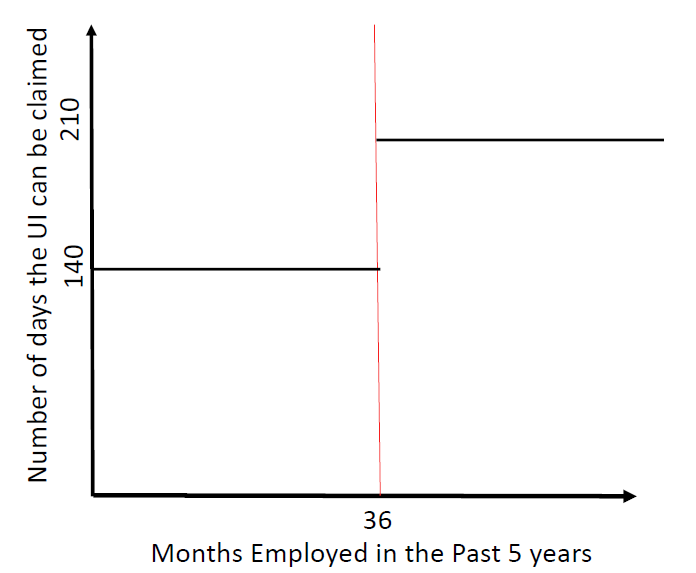
\includegraphics[width=2in]{images/ch1/card_1.png}%[scale option]{path and file name of the figure}
                \caption{an example}%caption
                \label{fig:label}%label for referencing. No need to include this if you don't need to refer back
            \end{figure}
Code:\\
\verb|\begin{figure}[H]%option [H] means "strictly here"|\\
\verb|\centering|\\
\verb|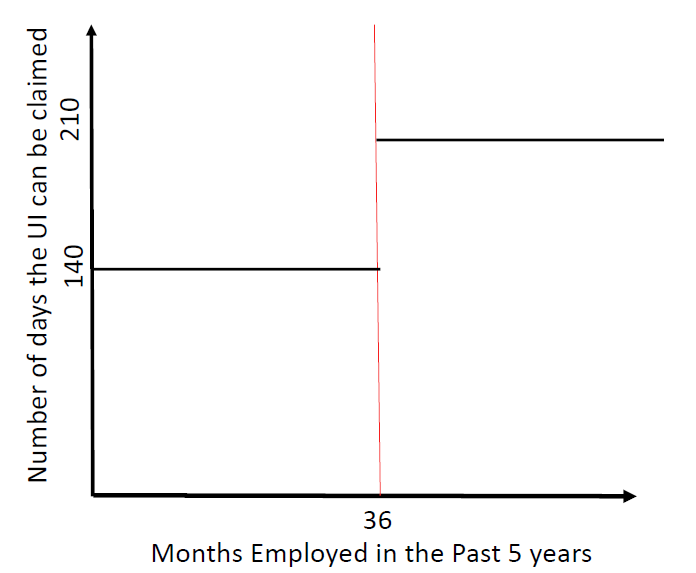
\includegraphics[width=2in]{images/ch1/card_1.png}%[scale option]{path and file name}|\\
\verb|\caption{an example}%caption|\\
\verb|\label{fig:label}%label for referencing. No need to include this if you don't need to refer back|\\
\verb|\end{figure}|









\section{123123}


    \begin{itemize}
        \item this is an item
        \item this is another item
        \begin{itemize}
            \item another
        \end{itemize}
    \end{itemize}

    \begin{enumerate}
        \item 12
        \item sjaiwjiodajo
    \end{enumerate}

    \begin{equation}
        x+y
    \end{equation}

    \begin{equation*}
        x+y
    \end{equation*}

    $$x+y$$

    this fraction $\frac{a}{b}$

    \begin{figure}[H]
        \centering
        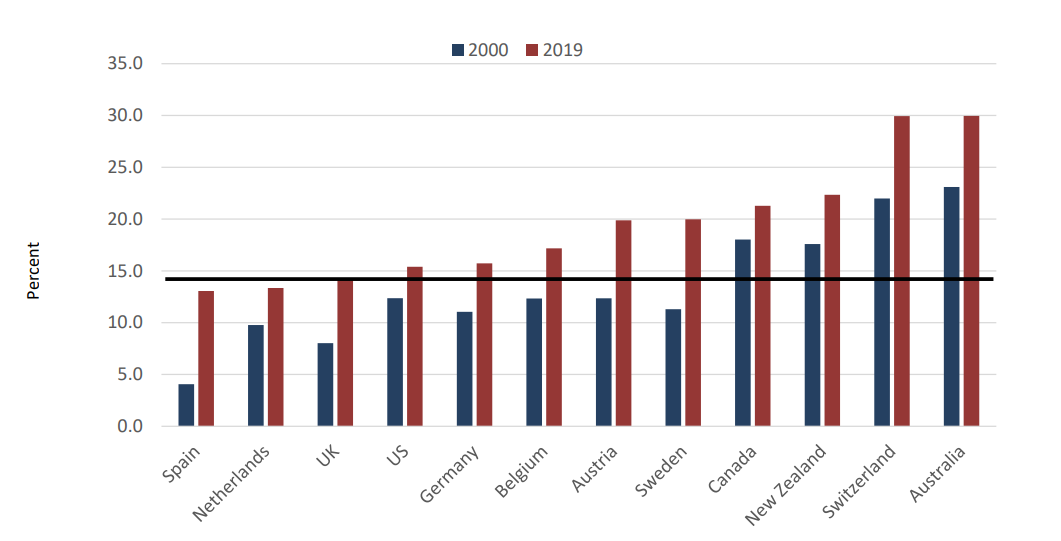
\includegraphics[width=4.5in]{images/ch11/2.png}
        \caption{This is a graph}
        \label{123123}
    \end{figure}

    \ref{123123}
\chapter*{Introduction}
These are our \empha{unofficial} lecture notes for \emphb{ECON0024 Economic Policy Analysis}. Contents are created according to professors' slides and lectures. Please contact me  (xiaotian.tian.20@ucl.ac.uk) should you have any questions or suggestions.

Remark on notations:
\begin{itemize}
    \item $\star$ indicates chapters that are ``model-intensive''
    \item \empha{Red highlights} usually indicate important conclusions and results
    \item \emphb{Blue highlights} usually indicate important concepts
\end{itemize}

Remarks:
\begin{itemize}
    \item \empha{Some contents are subject to our personal interpretations.}
    \item This is an open-source project. Contributions are welcomed!\\Github repository: \url{https://github.com/Er1kKa-Tian/ECON0024-Notes}
\end{itemize}



%I will probably delete this pic later :D
\iffalse
    \begin{figure}[H]
        \centering
        \includegraphics[scale=0.1]{images/102115356_p0.jpg}
        \caption{Enjoy this lovely picture before we start!}
        \label{fig:Introduction}
    \end{figure}
\fi

%Topic 1: UI and MW
\iftrue %Replace "iffalse" by "iftrue" if you want to render these chapters
    \chapter{Unemployment Insurance}

\fancyhead[L]{ECON0024}
\fancyhead[C]{Ch.1 Unemployment Insurance}
\fancyhead[R]{Xiaotian Tian}
\fancyfoot[L]{\hyperlink{tableofcontents}{Back to Table of Contents}}
\fancyfoot[R]{Xiaotian Tian}

\section{Unemployment}

    \subsection{Definition of Unemployment}
        The International Labour Organisation (ILO)'s \emphb{definition of unemployment}: The number of jobless people who want to work, are available to work, and are actively seeking employment
        
    \subsection{Why we care about unemployment?}
        \begin{enumerate}
            \item Unemployment is a sign of \emphb{inefficiency}.
            \item Modern view: part of the unemployment arises from \emphb{search costs (or frictions)}.
                \begin{itemize}
                    \item Zero unemployment is sub-optimal, because it indicates intensive job searching that induces high search costs.
                    \item Therefore, some level of unemployment (usually 3\% - 6\%) are tolerated in reality
                \end{itemize}
            \item Being unemployed decreases life satisfaction.
        \end{enumerate}

\section{Introduction to Unemployment Insurance (UI)}

    \subsection{Introduction}
        Many countries have some kind of UI, but it still remains controversial due to its benefit-and-cost \emphb{tradeoff}:
        \begin{itemize}
            \item Main benefit: helps people in a time of need
            \item Main cost: reduces incentive to search for work while unemployed
        \end{itemize}
        The following section will analyse how to design unemployment insurance given this trade-off.
        
    \subsection{Brief History of Unemployment Insurance}
        \begin{itemize}
            \item The first unemployment benefit scheme was introduced in the UK with the \textit{National Insurance Act} in 1911.
            \item U.S. introduced UI in 1935 in response to the Great Depression.
            \item Most European countries introduced UI after the WWII during the expansion of welfare state.
            \item Today, most developed countries have some UI schemes.
        \end{itemize}
        
    \subsection{Institutional Details}
        Typically, UI is financed through a payroll tax on employers and/or employees, but the incidence and rates vary a lot across countries. In exchange of the paid in contributions, unemployment benefit are received upon job-loss.
        \begin{itemize}
            \item Usually, the eligibility for UI must be a result of a layoff.
            \item The length and the level of UI benefits often depend on the amount and time length of contribution.
            \item Minimum contribution period and minimum contribution amount are often defined.
        \end{itemize}
        
    \subsection{Net Benefit Replacement Rate}
        We define the \emphb{Net Benefit Replacement Rate}, an important feature of UI, as:
        $$\text{Net\ Benefit\ Replacement\ Rate} = \frac{\text{Weekly\ Benefit}}{\text{Weekly\ Wage\ Earnings}}$$
        
\section{$\star$ Optimal Unemployment Insurance with No Moral Hazard}

    \subsection{Expected Utility Model of Unemployment}
        A typical objective considered by economist is to maximize agents' welfare given by expected utility.
        
        Specifically, we can calculate the \emphb{expected utility} by:
        $$E[U] = (1-p)\times{U(c^e)} + p\times{U(c^u)} - \psi(1-p)$$
        where
        \begin{itemize}
            \item $p$ is the probability of being \emph{unemployed} ("unemployment rate")
            \item $1-p$ is the probability of being \emph{employed}
            \item $c^u$ is the consumption when being \emph{unemployed}
            \item $c^e$ is the consumption when being \emph{employed}
            \item $U(.)$ is the utility function: we assume it to be \emph{strictly increasing and concave} i.e. $U'(.)>0$ and $U''(.)<0$
            \item $\psi(.)$ is the job searching cost function: we assume it to be \emph{strictly increasing and convex} i.e. $\psi'(.)>0$ and $\psi''(.)>0$
        \end{itemize}
        
            \subsubsection{Assumptions on the individual side}
                Assume \emphb{no saving/borrowing}:
                \begin{itemize}
                    \item Consumption at employment equals to after-tax wage i.e. $c^e = w-t$
                    \item Consumption at unemployment equals to UI benefit i.e. $c^u = b$
                \end{itemize}
                With this assumption, we can express the \emph{expected utility} as:
                \begin{equation}
                    E[U] = (1-p)\times{U(w-t)} + p\times{U(b)} - \psi(1-p)
                    \label{eqn:ui_exp_utility}
                \end{equation}
                
            \subsubsection{Assumptions on the government side:}
                Assume that the government must have a \emphb{balanced budget}: total tax collected must equal to total benefit given. With this assumption, we can write the government's \emphb{budget constraint}:
                $$(1-p)\times{t} = p\times{b}$$
                Rearranging this equation, it indicates that taxes need to be:
                $$t = \frac{p}{1-p}\times{b}$$
                plug these results into the expected utility of individuals (equation \ref{eqn:ui_exp_utility}):
                $$E[U] = (1-p)\times{U(w-\frac{p}{1-p}\times{b})} + p\times{U(b)} - \psi(1-p)$$
                Therefore, we can express the \emphb{government's optimisation problem} as:
                \begin{equation}
                    \label{eqn:ui_no_mh}
                    \max_{b} E[U] = (1-p)\times{U(w-\frac{p}{1-p}\times{b})} + p\times{U(b)} - \psi(1-p)
                    \end{equation}
                    
            \subsubsection{Further assumption: No moral hazard}
                Assume that $p$, the probability of finding a job, does not depend on the benefit level $b$, i.e. \emphb{no moral hazard}. We can treat $p$ as an exogenous variable here.
                
                \emph{Reminder: here, moral hazard refers to the adverse actions taken by insured individuals in response to insurance against adverse outcomes. It exists as long as insurers cannot perfectly monitor insurees.}
                
        \subsection{Optimisation Result: Full Insurance}
            To find the optimal UI, we solve the optimisation problem (\ref{eqn:ui_no_mh}). The FOC is:
            $$\frac{\partial E[U]}{\partial b}=-(1-p)\times{\frac{p}{1-p}}\times{U'(w-\frac{p}{1-p}\times{b})} + p\times{U'(b)} = 0$$
            $$U'(b) = U'(w-\frac{p}{1-p}\times{b})$$
            $$\color{red} b = w-\frac{p}{1-p}\times{b}$$
            This result implies that
            \[\color{red} c^e = w-t = b = c^u\]
            which indicates \emphb{full insurance} -- people have the same income when unemployed as they were employed. In practice, this would mean that the net replacement rate = 1. (\empha{No moral hazard $\leadsto$ Full insurance})
            
\section{$\star$ Optimal Unemployment Insurance with Moral Hazard}

    \subsection{Moral Hazard}
        The problem with full insurance is that it eliminates incentives to work. To incorporate \emphb{moral hazard} into our framework, we assume that $p$ increases with $b$: more generous benefits deter job search and hence increase unemployment.
        $$p=p(b),\ \frac{\partial p(b)}{\partial b}>0$$
        
    \subsection{Individuals' Response}
        Now, individuals choose their probability of being unemployment $p$ given the unemployment benefit $b$:
        $$\max_p E[U] = (1-p)\times{U(c^e)} + p\times{U(c^u)} - \psi(1-p)$$
        The FOC of this problem is:
        $$\frac{\partial E[U]}{\partial p}=-U(c^e)+E(c^u)+\psi'(1-p) = 0$$
        Manipulate:
        $$Pr(employed) = 1-p = \psi'^{-1}\Big(U(c^e)-U(c^u)\Big)$$
        Note that $c^e, c^u$ are also functions of $b$:
        \begin{equation}
            \label{eqn:ui_mh_optimal_p}
            Pr(employed) = 1-p(b) = \psi'^{-1}\Big(U(w-\frac{p}{1-p}\times{b})-U(b)\Big)
        \end{equation}
        Now, we can investigate the effect of changing $b$ on the probability of being employed (using $\frac{\partial f^{-1}(x)}{\partial x} = \frac{1}{f'(x)}$):
        $$\frac{\partial Pr(employed)}{\partial b}=\frac{\partial(1-p(b))}{\partial b} = \frac{-\frac{p}{1-p}\times{U'\big(w-\frac{p}{1-p}\times{b}\big)}-U'(b)}{\psi''\Big(U\big(w-\frac{p}{1-p}\times{b}\big)-U(b)\Big)} < 0$$
        because $U'(.)>0$ and $\psi''(.)>0$ by assumption.
        
    \subsection{The government's optimisation: Partial Insurance}
        Our model now becomes:
        $$\max_b E[U] = \big(1-p(b)\big)\times{U\left(w-\frac{p(b)}{1-p(b)}\times{b}\right)} + p(b)\times{U(b)} - \psi\big(1-p(b)\big)$$
        The FOC becomes more complicated:
        $$0 = -U'\left( w-\frac{p(b)}{1-p(b)}\times{b} \right)\times{\left(\frac{p'(b)\times{b}}{1-p(b)}+p(b)\right)} + p(b)U'(b) + p'(b)\times\underbrace{\big[-U(c^e)+U(c^u)+\psi'(1-p(b))\big]}_{\text{From\ the\ FOC\ of\ individuals,\ we\ know\ this\ is\ 0}}$$
        $$0 = -U'\left(\underbrace{ w-\frac{p(b)}{1-p(b)}\times{b} }_{c^e}\right)\times{\left(\frac{p'(b)\times{b}}{1-p(b)}+p(b)\right)} + p(b)U'(\underbrace{b}_{c^u})$$
        Rearrange this, we can get the \empha{Main Equation of Optimal UI}:
        \begin{equation}
            \label{eqn:ui_mh_main}
            \color{red}
            \underbrace{\frac{U'(c^u)-U'(c^e)}{U'(c^e)}}_{\text{Insurance\ Value}} = \underbrace{\frac{1}{1-p}\times{\epsilon_{p,b}}}_{\text{Moral\ Hazard\ Cost}}
        \end{equation}
        where $\epsilon_{p,b} = \frac{b}{p}\frac{dp}{db}$ is the \emphb{elasticity of unemployment rate with respect to benefits}.
        
        Note that the Main Equation of Optimal UI implies: if $\epsilon_{p,b}>0$, then $0<c^u<c^e<w$ which means \emphb{partial insurance} will be the optimum. (\empha{Moral hazard $\leadsto$ Partial insurance})
        
    \subsection{Explaining the Main Equation of Optimal UI}
        As in a typical optimum, the marginal benefit (insurance value) has to be equal to the marginal cost (moral hazard cost). If the marginal benefit (insurance value) is larger than the marginal cost (moral hazard cost), we need to increase the UI benefit to reach optimum, v.v.
        \begin{enumerate}
            \item \textbf{\emphb{Insurance Value}}\\
            This is the marginal benefit of UI benefit (redistributing one unit from the employed to the unemployed): if we increase the UI benefit by 1 unit, the net benefit will be the insurance value:
            $$\text{Insurance\ Value} = \frac{U'(c^u)-U'(c^e)}{U'(c^e)}$$
            \item \textbf{\emphb{Moral Hazard Cost}}\\
            This is the marginal cost of UI benefit (redistributing one unit from the employed to the unemployed): if we want to increase the UI benefit by 1 unit, we need to collect an extra of: $p(b) + p'(b)\times b$. This has to be paid by people who remain employed, so the tax rate has to increase by: $\frac{p(b)+p'(b)\times{b}}{1-p(b)}$. Rearrange:
            $$\text{Moral\ Hazard\ Cost} = \frac{p(b)}{1-p(b)}\times\left(1+p'(b)\times\frac{b}{p(b)}\right) = \frac{p(b)}{1-p(b)}\times(1+\epsilon_{p,b})$$
            This can be understood as the extra cost imposed on an employed individual in order to redistribute 1 unit to every unemployed individual. The more responsive the unemployment rate is (higher $\epsilon_{p,b}$), the more costly of an increase in UI will be.
        \end{enumerate}
        
    \subsection{Sufficient Statistic Approach}
    
        \subsubsection{Approximate the Main Equation of Optimal UI}
            The term $\frac{U'(c^u)-U'(c^e)}{U'(c^e)}$ cannot be estimated because people's utility functions are not observed. In stead, we employ the 1st order Taylor Expansion. Expand $U'(c^u)$ around $c^e$:
            $$U'(c^u) \approx U'(c^e) + U''(c^e)(c^u-c^e)$$
            Therefore:
            \begin{equation*}
                \begin{split}
                \frac{U'(c^u)-U'(c^e)}{U'(c^e)} & \approx \frac{U'(c^e) + U''(c^e)(c^u-c^e)-U'(c^e)}{U'(c^e)}\\
                & = \frac{U''(c^e)(c^u-c^e)}{U'(c^e)}\\
                & = \underbrace{-\frac{c^e U''(c^e)}{U'(c^e)}}_{\text{Relative\ Risk\ Aversion}\ \gamma} \times \frac{c^e-c^u}{c^e}\\
                & = \gamma \times \frac{c^e-c^u}{c^e}\\
                & = \gamma \times \frac{\Delta c}{c^e}
            \end{split}
            \end{equation*}
            Substituting this into the main equation (\ref{eqn:ui_mh_main}):
            \begin{equation}
            \label{eqn:ui_hm_sufficient}
            \color{red}
                \underbrace{\frac{1}{1-p}\times{\epsilon_{p,b}}}_{\text{Moral\ Hazard\ Cost}} \approx \underbrace{\gamma \times \frac{\Delta c}{c^e}}_{\text{Insurance\ Value}}
            \end{equation}
            This equation (\ref{eqn:ui_hm_sufficient}) is a transformation of the Main Equation of Optimal UI, which is estimable in practice:
            \begin{itemize}
                \item $\frac{\Delta c}{c^e}$ is the consumption drop at unemployment
                \item $\gamma$ is the coefficient of relative risk aversion (higher RRA indicates more risk aversion)
                \item $\epsilon_{p,b} = \frac{b}{p}\frac{dp}{db}$ is the elasticity of unemployment rate with respect to benefits
            \end{itemize}
            We call this the \emphb{Sufficient Statistic Approach} because the optimal UI can be calculated aftering measuring the above three factors.
            
        \subsubsection{Pros and Cons of the Sufficient Statistic Approach}
            The alternative method of determining the optimal UI benefit is known as the \emphb{structural labour approach}:
            \begin{enumerate}
                \item Estimate the key parameters of the utility function, job search function, etc.
                \item Simulate counterfactual results with alternative levels of the UI benefit
            \end{enumerate}
            The first procedure often requires functional assumptions on the utility function and the cost of job search. Compared with this, the Sufficient Statistic Approach focus on some key statistics without identifying the whole model of job search. Thus, it has obvious pros and cons:
            \begin{itemize}
                \item \textbf{Key advantage}: easier to implement and less assumptions are needed
                \item \textbf{Key disadvantage}: the derivation of the Main Equation of Optimal UI depends critically on the \emph{envelop theorem} which only holds for small policy deviations (and we used the 1st order Taylor Expansion, which is a local approximation), so it cannot be used to assess the impact of radical changes
            \end{itemize}

\section{Estimation of Moral Hazard ($\epsilon_{p,b}$)}
    Moral hazard in UI is thought to manifest itself in the duration of unemployment: economists investigate whether unemployed individuals find jobs more slowly when UI benefits are higher. The key challenge is to use quasi-experiments to identify these effects.
    
    \subsection{Difference-in-Difference}
        The idea is to exploit changes in UI laws that affect a \emph{treatment} group and compare that with a \emph{control} group.
        \begin{figure}[h]
            \centering
            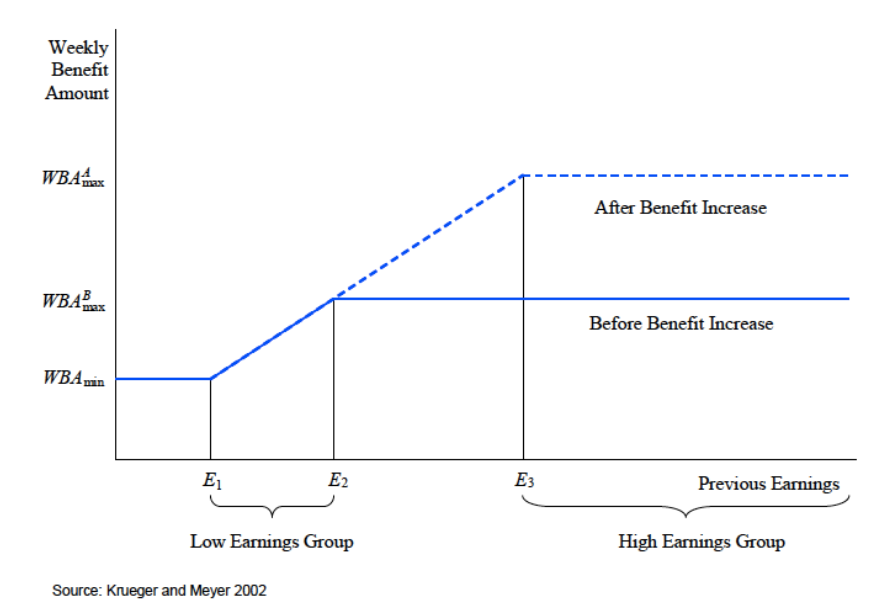
\includegraphics[width=4 in]{images/ch1/did_1.png}
            \caption{Example of DiD: low earnings group as control and high earnings group as treatment}
        \end{figure}
        \begin{enumerate}
            \item Standard DiD specification with 2 states and 2 time period
            $$log(Unemployment\ Duration)_{ist} = \beta_0 + \beta_1 After_{ist} + \beta_2 Treat_{ist} + \beta_3 Treat_{ist} \times After_{ist} + \epsilon_{ist}$$
            where:
            \begin{itemize}
                \item $log(Unemployment\ Duration)_{ist}$ is the log unemployment duration of individual i in state s at time t
                \item $After_{ist}$ is the time dummy
                \item $Treat_{ist}$ is the treatment dummy
            \end{itemize}
            Under the \emphb{Common/Parallel Trend Assumption} (the difference in unemployment duration would have been the same between the treatment/control group in absence of the policy change), $\beta_3$ identifies the casual effect (ATT, specifically).
            \item Fixed Effects Version\\
            $$log(Unemployment\ Duration)_{ist} = \alpha_s + \theta_t + \beta log(b_{ist}) + \gamma X_{ist} + \epsilon_{ist}$$
            where:
            \begin{itemize}
                \item $\alpha_s$ is the state fixed effect
                \item $\theta_t$ is the time fixed effect
                \item $X_{ist}$ includes other control variables
            \end{itemize}
            $\beta$ identifies the relationship between percentage change in replacement rate and percentage change in unemployment duration under FE/FD assumptions. (Correct specification; Random sampling; Time variations and no perfect multicolinearity in regressors; Zero conditional mean)\\
            Meyer (1990) and many other implement this method using data on unemployment duration in the U.S. and state-level reforms. The general finding shows a \empha{benefit elasticity of 0.4-0.6}: 10\% rise in unemployment benefits leads to about a 4-6\% increase in unemployment duration.
        \end{enumerate}
            
    \subsection{Regression Discontinuity Designs}
        This empirical strategy exploits jumps in UI benefits at a threshold.
        \emph{\textbf{Main assumption}}: \emphb{Continuity}: individuals who are slightly below the threshold and individuals who are slightly above the threshold would have similar unemployment duration in absence of the jump in the UI benefit level at the threshold.
        
        This assumption will not hold if:
        \begin{itemize}
            \item There are \emph{selection/manipulation} on one side of the threshold. For example, the unemployed somehow achieve to lay-off a few days to deliberately reach the threshold.
            \item There are other policy changes that affect outcomes at the threshold.
        \end{itemize}
        Example:\\
        Card-Chetty-Weber (2007) used the fact that in Austria, you get up to 30 weeks of benefits when you have been employed for 36+ months in last 5 years (instead of up to 20 weeks).
        \begin{figure}[H]
            \centering
            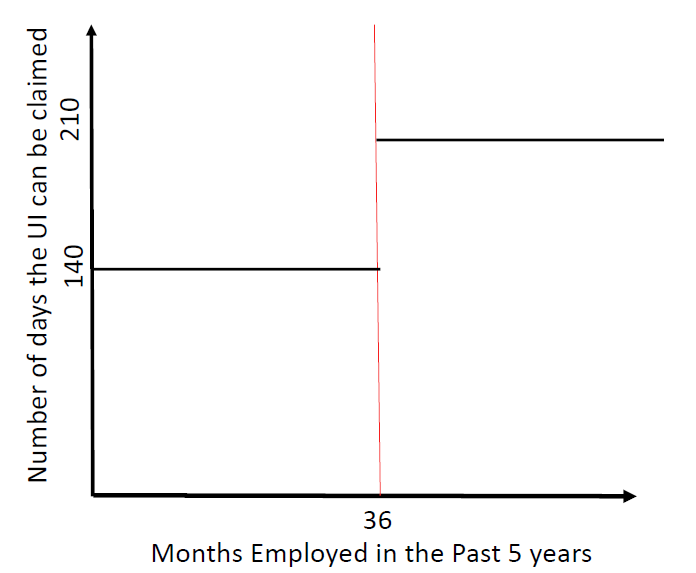
\includegraphics[width=3 in]{images/ch1/card_1.png}
            \caption{Jump in UI Benefit}
            \label{fig:card_1}
        \end{figure}
        They checked: (1) there is no selection around the threshold (on frequency of layoffs, age, wages, etc.) (2) there is no other policy change at the threshold.
        \begin{figure}[H]
            \centering
            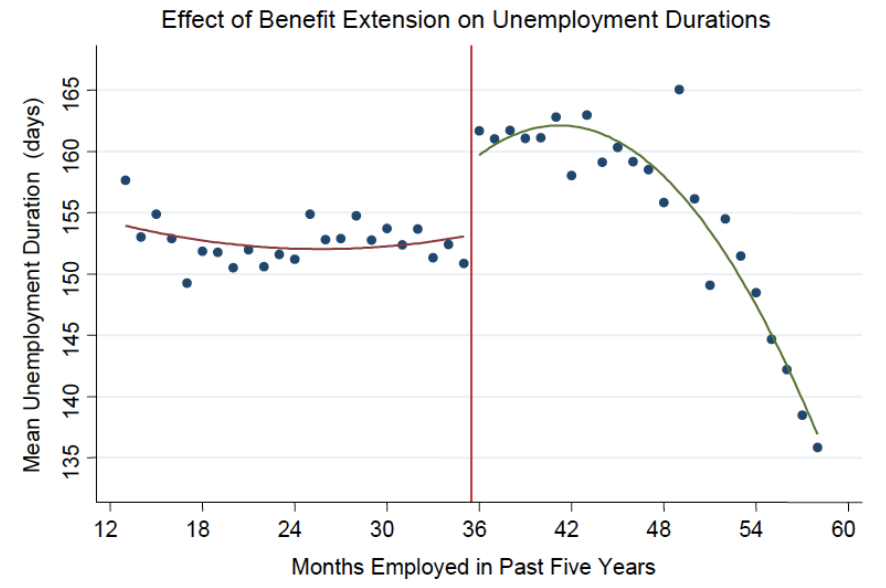
\includegraphics[width=4 in]{images/ch1/card_2.png}
            \caption{RDD Result}
            \label{fig:card_2}
        \end{figure}
        They estimated a benefit elasticity $\epsilon_{p,b} \approx 0.3$.
        
    \subsection{Regression Kink Designs}
        This strategy is very similar to RDD, but we exploit a kink in UI benefits instead of a jump.
        \emph{\textbf{Main assumption}}: In the absence of the kink in the benefit-level, there would be no kink in unemployment duration.\\
        Example:\\
        Kolsrud, Landais, Nilsson and Spinnewijn (2016) studied a kinked UI benefit scheme in Sweden from 1999 to 2000:
        \begin{figure}[H]
            \centering
            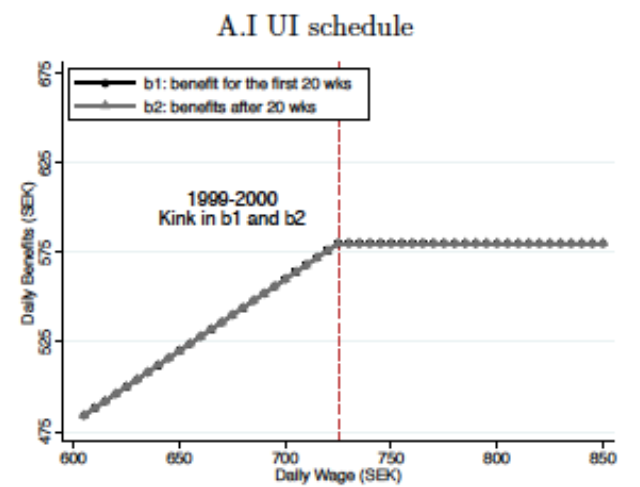
\includegraphics[width = 3 in]{images/ch1/RKD_1.png}
            \caption{Kinked UI Benefits}
            \label{fig:RKD_1}
        \end{figure}
        They found a kink in unemployment duration, indicating the existence of moral hazard:
        \begin{figure}[H]
            \centering
            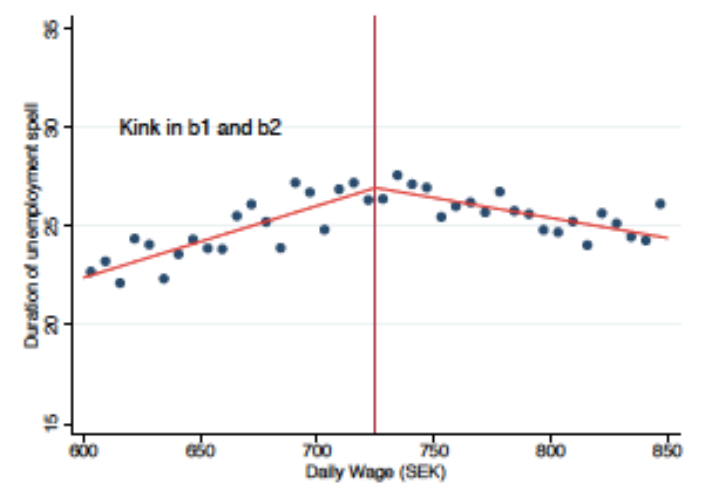
\includegraphics[width = 3 in]{images/ch1/RKD_2.png}
            \caption{Kinked Unemployment Duration}
            \label{fig:RKD_2}
        \end{figure}
        In this case, the assumption can be easily checked: after 2000, the kinked UI benefits was abandoned, and the kink in unemployment duration disappeared:
        \begin{figure}[H]
            \centering
            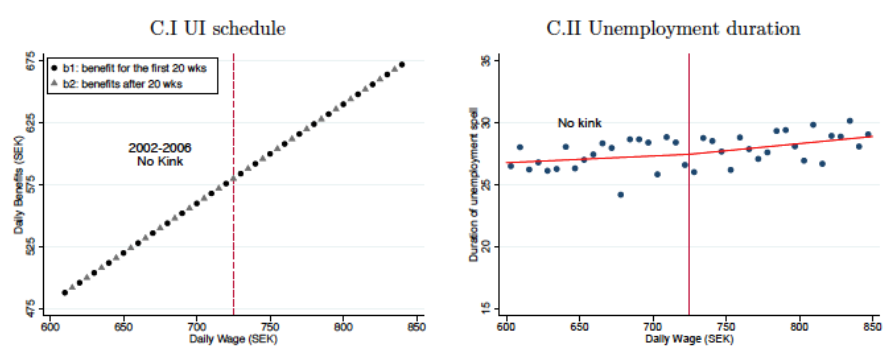
\includegraphics[width = 6 in]{images/ch1/RKD_3.png}
            \caption{Check the Assumption}
            \label{fig:RKD_3}
        \end{figure}
        
        \subsection{Extension: Decompose the Effect Using the Slutsky Equation}
            \subsubsection{Decomposition}
                Similar to the Slutsky Equation, we can decompose the overall effect of changes in UI benefit on job research of the unemployed into a liquidity effect and a moral hazard effect (discussed by Card, Chetty, and Webers (2007)):
                $$\underbrace{\frac{\partial s_t}{\partial b_t}}_{\text{Overall\ Effect}} = \underbrace{\frac{\partial s_t}{\partial A_t}}_{\text{Liquidity\ Effect}} - \underbrace{\frac{\partial s_t}{\partial w_t}}_{\text{Moral\ Hazard\ Effect}}$$
                where:
                \begin{itemize}
                    \item Liquidity Effect shows how search would change if cash was given to the agent independently of being unemployed or not -- giving an extra dollar of UI benefits increases the wealth of the receiver, making them feel "richer."
                    \item Moral Hazard Effect shows the distortion effect of UI benefit -- giving an extra dollar of UI benefit distorts the "price" of being unemployed compared with being employed, i.e. the receiver may have lower incentives to look for a job.
                \end{itemize}
            \subsubsection{Estimation Using Two RDD}
                Card et. al. (2007), estimated the overall effect and liquidity effect, then calculated the moral hazard effect using the above decomposition.
                \begin{itemize}
                    \item Estimating Overall Effect: RDD exploiting the fact that people with less than 36 months of employment in the past 5 years receive 20 rather than 30 weeks of UI. Compare non-employment duration of those just below the 36 months threshold and those just above it.
                    \item Estimating Liquidity Effect: RDD exploiting the fact that firms are forced to pay a lump-sum severance payment equal to 2 months of previous salary to workers who are laid off after 3 years of service. Compare workers who are just below the 3 year cutoff with those just above, and look at the difference in their non-employment duration.
                \end{itemize}
        
\section{Evidence on Consumption Smoothing ($\frac{\Delta c}{c^e}$)}
    The evidence on consumption smoothing is more limited. The key constraint is data: while we have millions of observations of unemployment duration (administrative records), data on consumption is often restricted to surveys, which contain much less samples. (Typically, we need a large sample size to use RDD/RKD.)
    
    \subsection{Difference-in-Difference}
        The settings are similar to the DiD strategy mentioned before. Gruber (1997) used food consumption as the dependent variable, and used cross-state and time variations. The dataset used is PSID food consumption.
        
        Gruber identified the following equation:
        $$\frac{\Delta c}{c^e} = \beta_0 + \beta_1 \frac{b}{w_i}$$
        
        Their results show that: $\beta_0 \approx 0.24$ and $\beta_1 \approx -0.28$. Without UI benefits, unemployment will cause a 24\% drop in consumption. With the current level of UI benefit (net benefit replacement rate $\frac{b}{w_i}=0.5$), the consumption is estimated to drop about 10\%, and a 10\% increase in UI benefits will induce a 2.8\% reduction in the consumption drop.
        
        This provides convincing evidence that insurance markets are not perfect and UI does play a consumption smoothing role.
        
        Note that the drop in benefit-level and the drop in consumption is much less than 1-1. This is because UI also affects people's \emphb{Self Insurance} behaviour:
        \begin{itemize}
            \item Saving behaviours
            \item Spousal labor supply
            \item Borrowing from friends
        \end{itemize}
        Provision of UI benefits crowds out such self insurance to some extent.
    
    \subsection{Using Data of Bank Accounts}
    
        Ganong (2016) uses JPMorgan Chase Institute’s (JPMCI) data on anonymized data on 210,000 checking accounts that received a direct deposit of unemployment insurance (UI) benefits. This overcomes the small sample problem present in survey data.
        \begin{figure}[H]
            \centering
            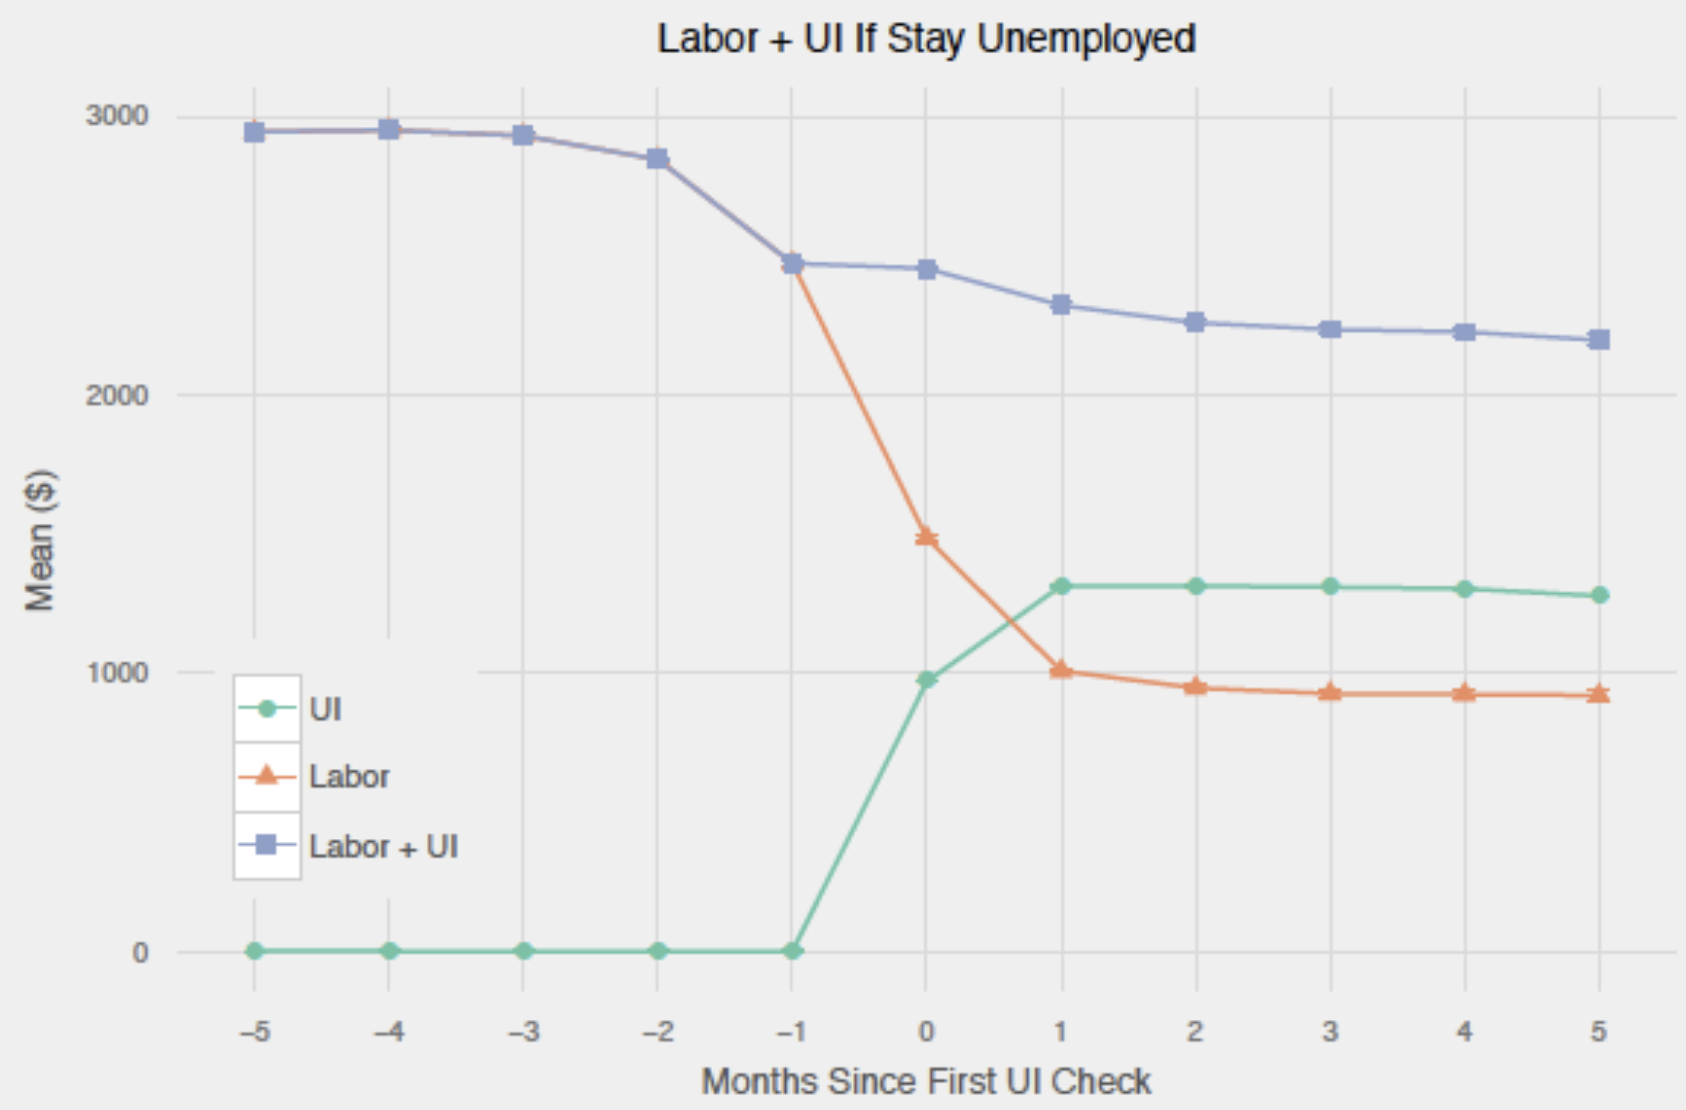
\includegraphics[width=4in]{images/ch1/Ganong_1.png}
            \caption{Labour Income and UI Benefits}
            \label{fig:Ganong_1}
        \end{figure}
        We can see a clear drop in individuals' disposable income after becoming unemployed.
        \begin{figure}[H]
            \centering
            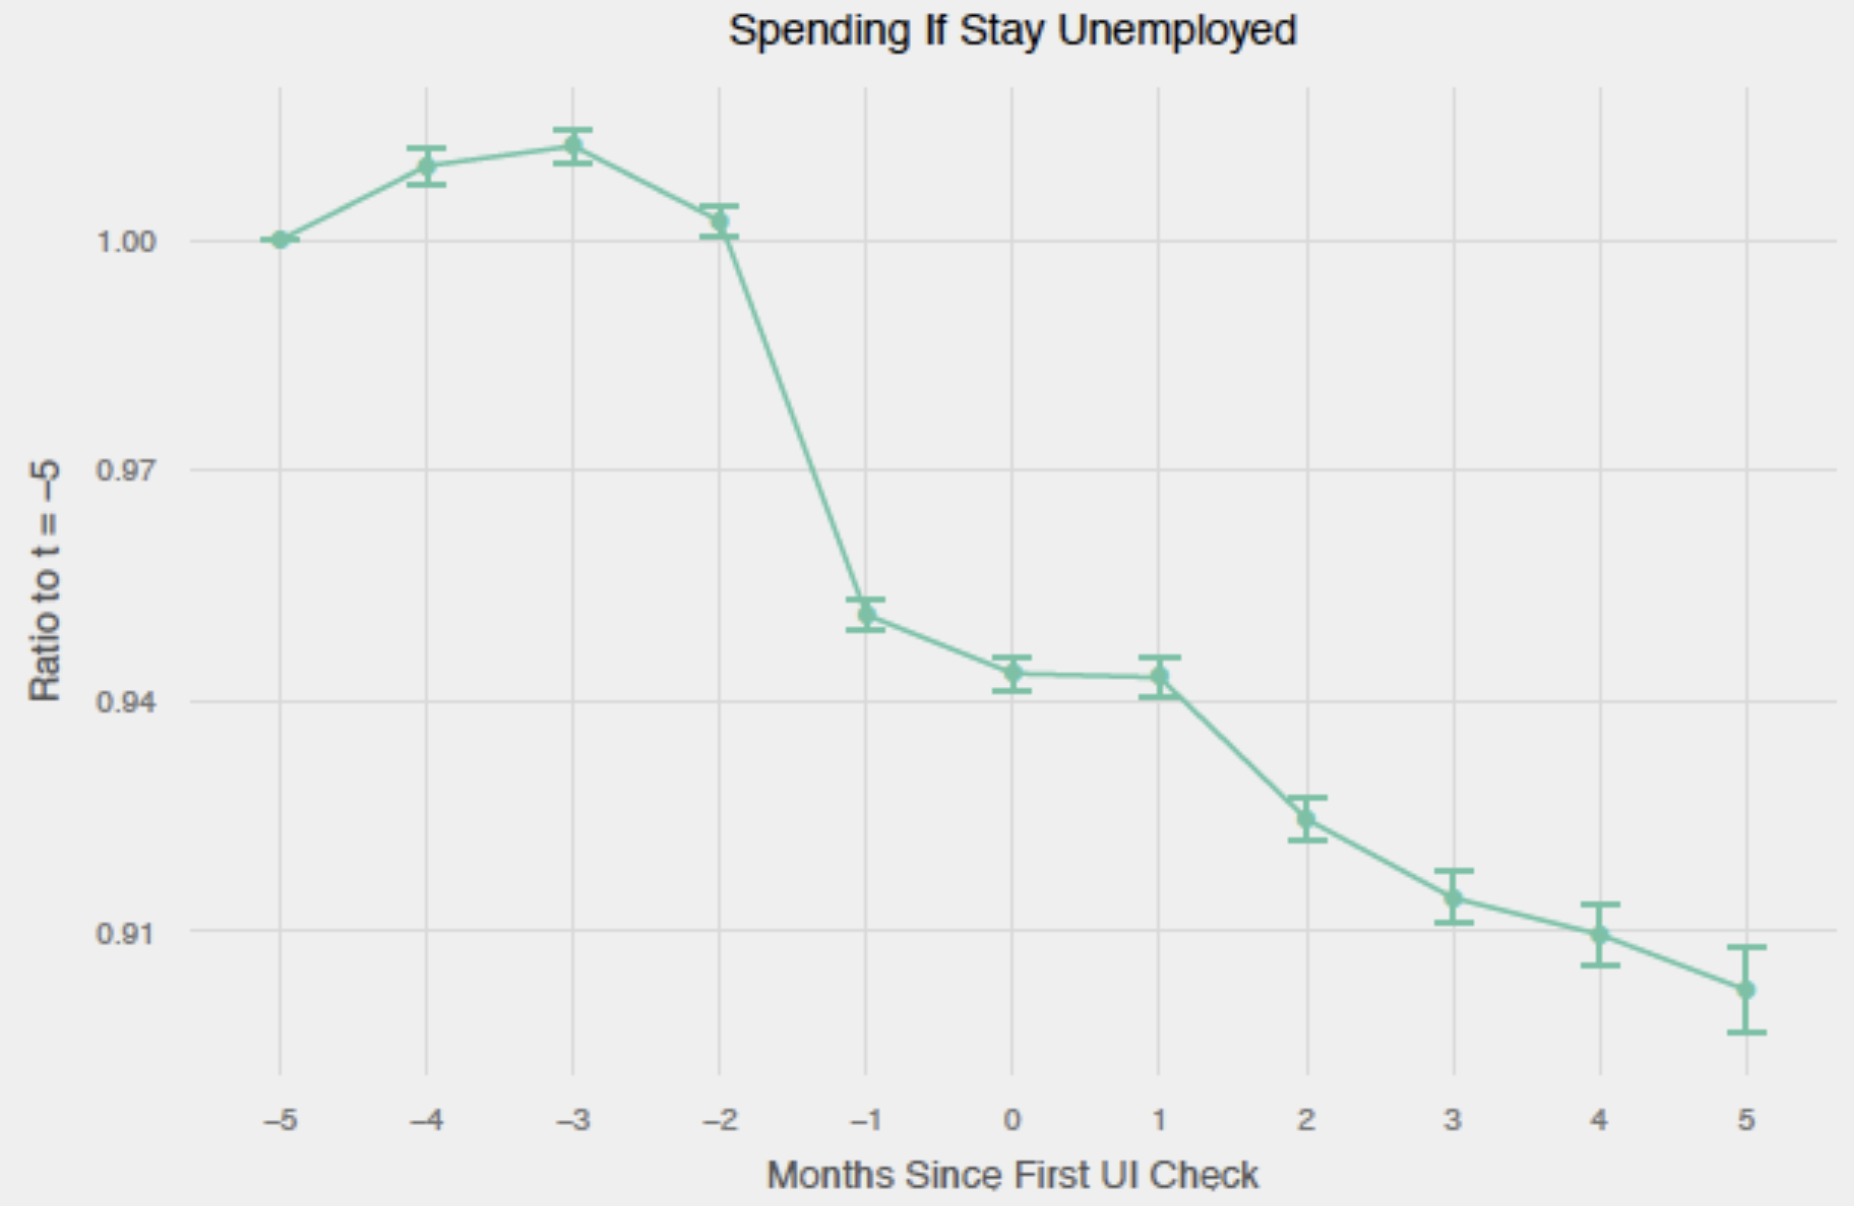
\includegraphics[width=4in]{images/ch1/Ganong_2.png}
            \caption{Spending if Individuals Stay Unemployed}
            \label{fig:Ganong_2}
        \end{figure}
        We can see that, if individuals stay unemployed, their spending will keep decreasing.
        \begin{figure}[H]
            \centering
            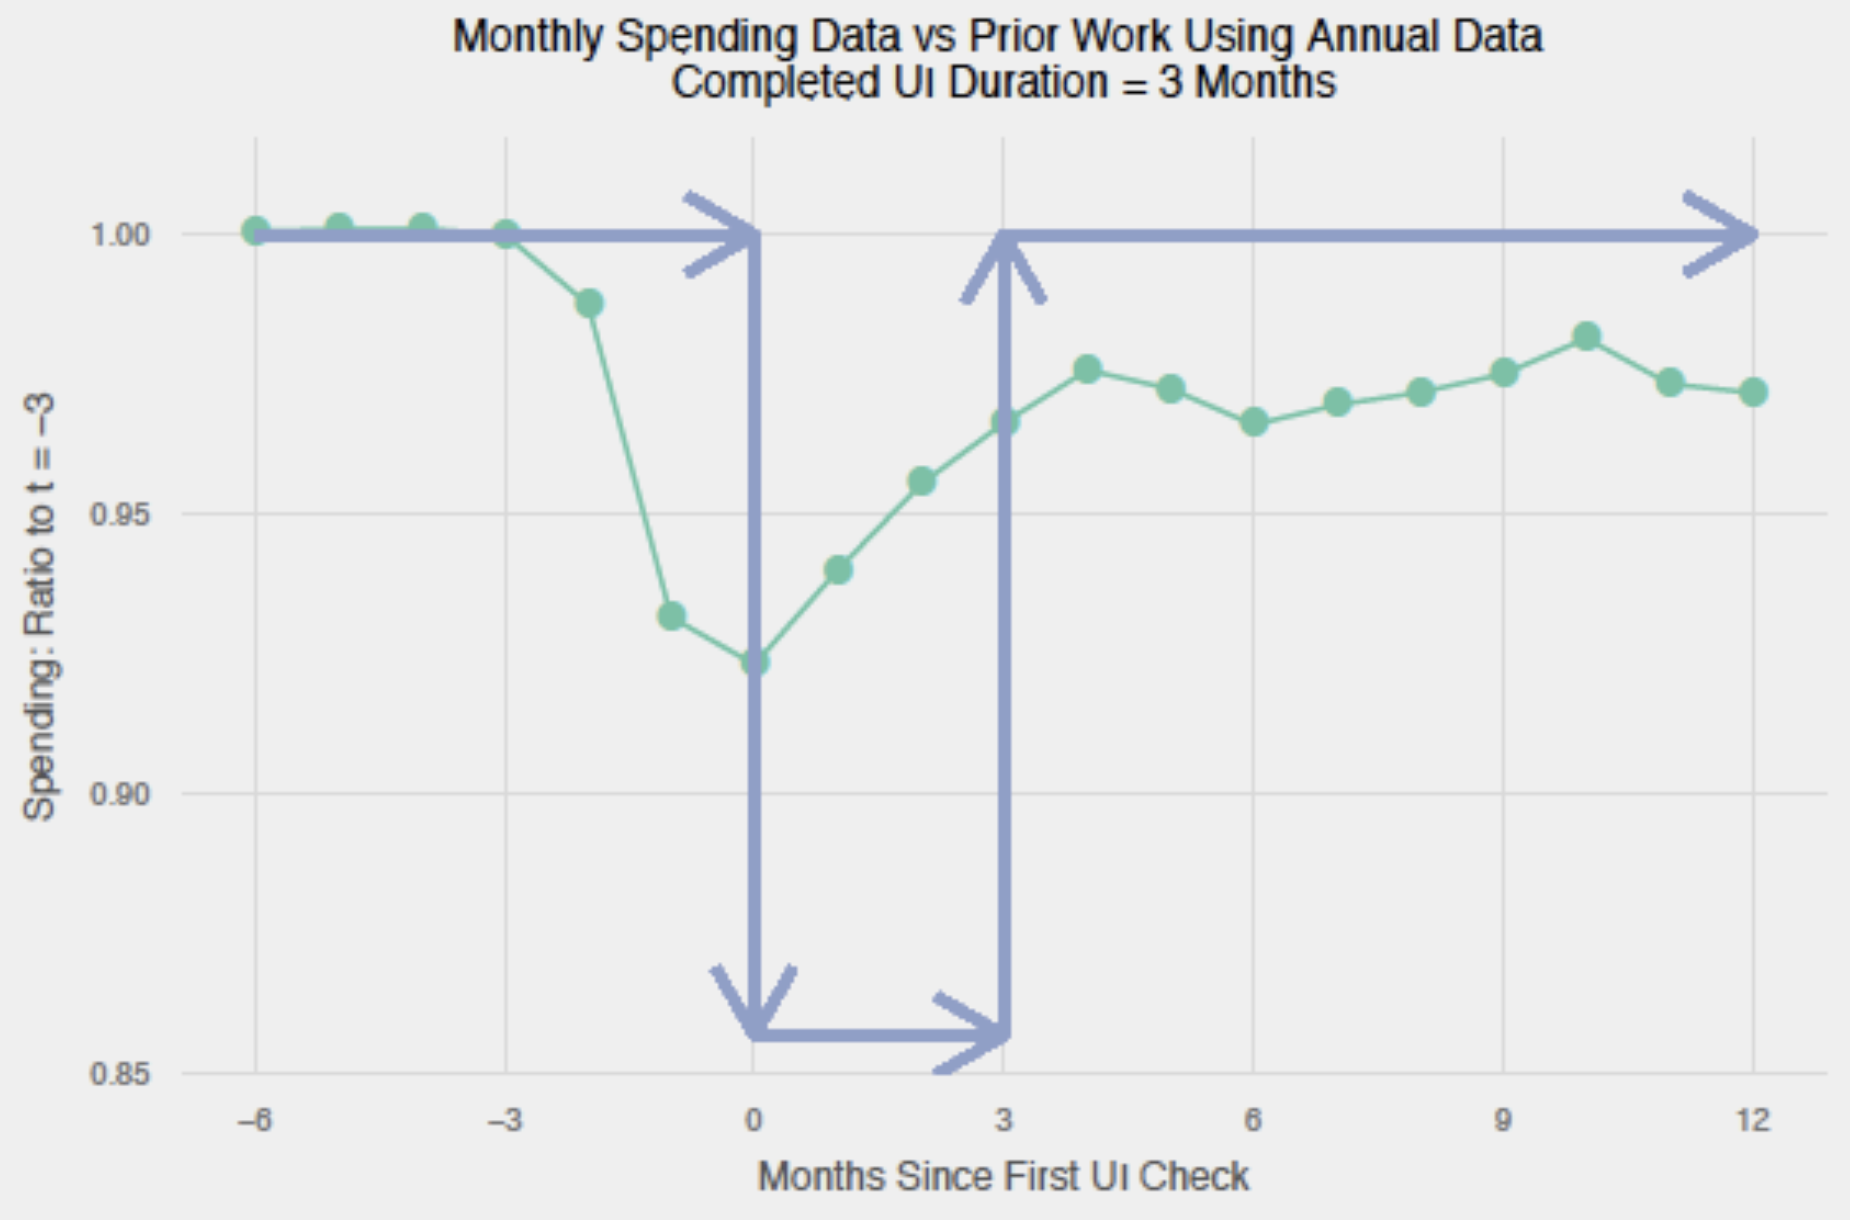
\includegraphics[width=4in]{images/ch1/Ganong_3.png}
            \caption{Spending if Individuals Find a Job after 3 Months}
            \label{fig:Ganong_3}
        \end{figure}
        However, if they find a job after 3 months, their consumption drop will be much less.
        \begin{figure}[H]
            \centering
            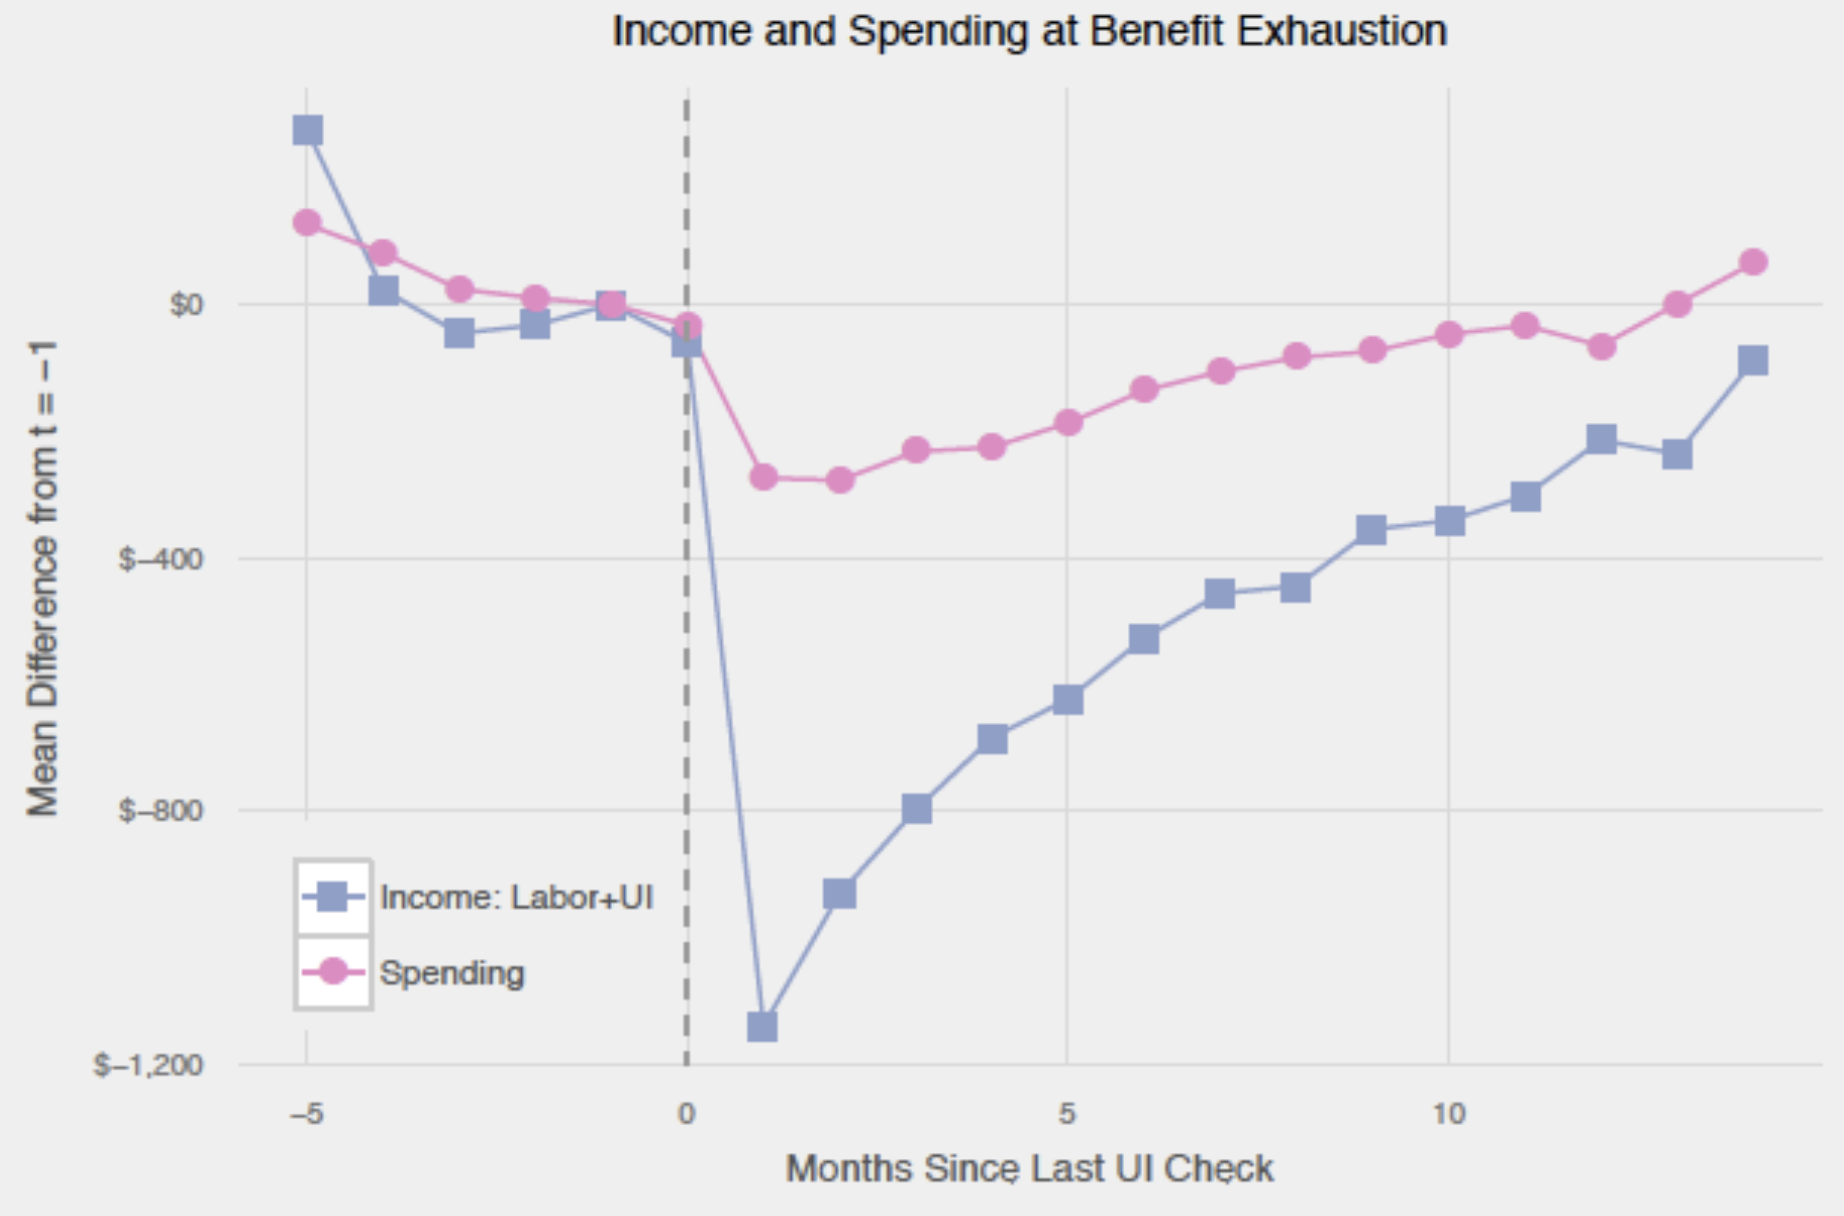
\includegraphics[width=4in]{images/ch1/Ganong_4.png}
            \caption{Consumption and Income Paths}
            \label{fig:Ganong_4}
        \end{figure}
        The figure above clearly indicates that, during unemployment, people are spending more than their income, suggesting that they are smoothing their consumption.
        
    \subsection{Using Administrative Data}
        Kolsrud, Landais, Nilsson and Spinnewijn (2016) uses administrative data on unemployment, which is linked to data on income and wealth in Sweden. They use income and wealth changes to create a registry-based consumption measure. Again, this overcomes the small sample problem present in survey data.
        \begin{figure}[H]
            \centering
            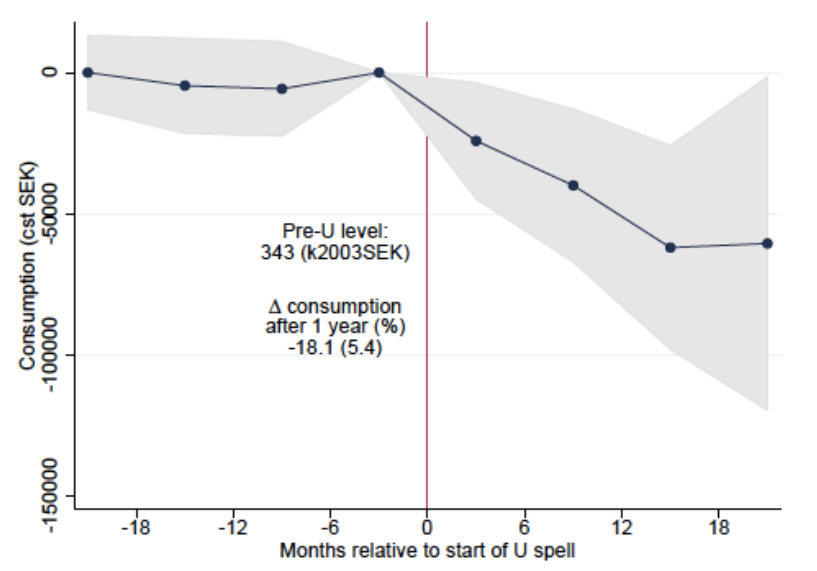
\includegraphics[width=4in]{images/ch1/Kolsrud_1.png}
            \caption{Kolsrud's Results}
            \label{fig:Kolsrudl}
        \end{figure}
        Their results also corroborated the existence of consumption smoothing.
        
\section{$\star$ Implication of the Empirical Evidence on the Optimal UI}
    
    \subsection{Is Our Current UI Benefit Optimal?}
        Recall our "sufficient statistical approach" version (equation \ref{eqn:ui_hm_sufficient}) of the Main Equation of Optimal UI:
        \begin{equation*}
        \color{red}
            \underbrace{\frac{1}{1-p}\times{\epsilon_{p,b}}}_{\text{Moral\ Hazard\ Cost}} \approx \underbrace{\gamma \times \frac{\Delta c}{c^e}}_{\text{Insurance\ Value}}
        \end{equation*}
        From our empirical researches:
        \begin{itemize}
            \item Consumption drop $\frac{\Delta c}{c^e}$ is around 10\%
            \item Elasticity of probability of unemployment with respect to UI benefit level $\epsilon_{p,b}$ is around 0.3
            \item The probability of being employed $(1-p)$ is around 90-95\%, depending on the state of the economy
            \item Survey results suggest an average RRA $\gamma$ around 2
        \end{itemize}
        Plug in those values:
        $$\underbrace{\frac{1}{0.95}\times{0.3} \approx 0.316}_{\text{Moral\ Hazard\ Cost}} > \underbrace{2 \times 0.1 = 0.2}_{\text{Insurance\ Value}}$$
        $$\text{Moral\ Hazard\ Cost} > \text{Insurance\ Value}\ \Rightarrow\ b>b^*$$
        Currently, the moral hazard cost is higher than the insurance value, indicating that our UI benefit level is too high (\emph{too generous}). We should cut the benefit level to optimize.
        
    \subsection{Counter-arguments by Chetty and Szeidl (2007): Consumption Commitment \& Risk Aversion}
        Chetty and Szeidl (2007) pointed out that risk aversion, $\gamma$, is poorly identified, and it appears to vary substantially according to specific situations. Specifically, people with consumption commitments tend to have higher risk aversion as explained below.
        \subsubsection{Consumption Commitment}
        Chetty and Szeidl extended the standard expected utility model to incorporate goods whose consumption is hard to adjust (e.g. mortgage).
        
        The standard utility model assumes that there is only one consumption good $c$, and people can cut back on all consumption goods freely anytime. This implies that, when unemployed, consumption of food, housing, cars, furniture... will all drop.
        
        However, in practice, it is hard to adjust many elements of consumption in short run due to adjustment costs.
        \begin{figure}[H]
            \centering
            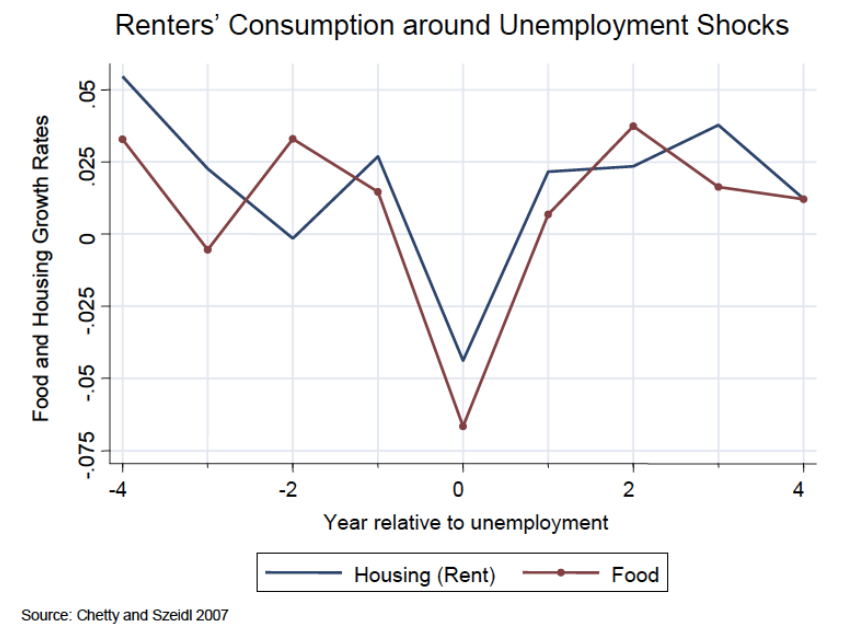
\includegraphics[width=4in]{images/ch1/Chetty_1.png}
            \caption{Consumption Commitment}
            \label{fig:Chetty}
        \end{figure}
        Shown above, compared with consumption on foods, rents are much harder to be cut off. Therefore, facing unemployment, individuals may need to reduce more flexible consumption, such as foods. In this case, the actual welfare loss will be greater.
        \subsubsection{Higher Risk Aversion}
        Chetty's model with consumption commitments suggests that risk aversion $\gamma$ may be greater than 4 when agents are hit by an unemployment shock, because consumption commitment amplifies negative utility effects, making people more dislike negative income shocks.
        
        Plugging in this value:
        $$\underbrace{\frac{1}{0.95}\times{0.3} \approx 0.316}_{\text{Moral\ Hazard\ Cost}} < \underbrace{4 \times 0.1 = 0.4}_{\text{Insurance\ Value}}$$
        $$\text{Moral\ Hazard\ Cost} < \text{Insurance\ Value}\ \Rightarrow\ b<b^*$$
        
        Therefore, under this more realistic model, our current UI benefit level is lower than the optimal level.
    
\section{Should UI Benefits Vary by the Business Cycle?}
    Our optimization requires equalization of insurance value and moral hazard cost, which contain parameters: $p, \epsilon_{p,b}, \frac{\Delta c}{c^e}, \gamma$. If they vary with the business cycle, our optimal UI benefits should adjust accordingly. Thus, again, this is an empirical question.
    
    \subsection{Unemployment Duration and the Business Cycle}
        Schmieder, von Wachter and Bender (2011) conclude that, during recessions:
        \begin{itemize}
            \item the responsiveness of unemployment duration to an additional month of UI benefit is lower. ($\frac{dp}{db}$ is lower)
            \item the probability of employment is lower ($p$ is lower) 
        \end{itemize}
        Therefore, the \empha{elasticity of unemployment rate with respect to benefits $\epsilon_{p,b}$ is lower in recessions}. This in turn indicates lower moral hazard costs, and UI benefits should be higher in recessions to optimise.
        \begin{figure}[H]
            \centering
            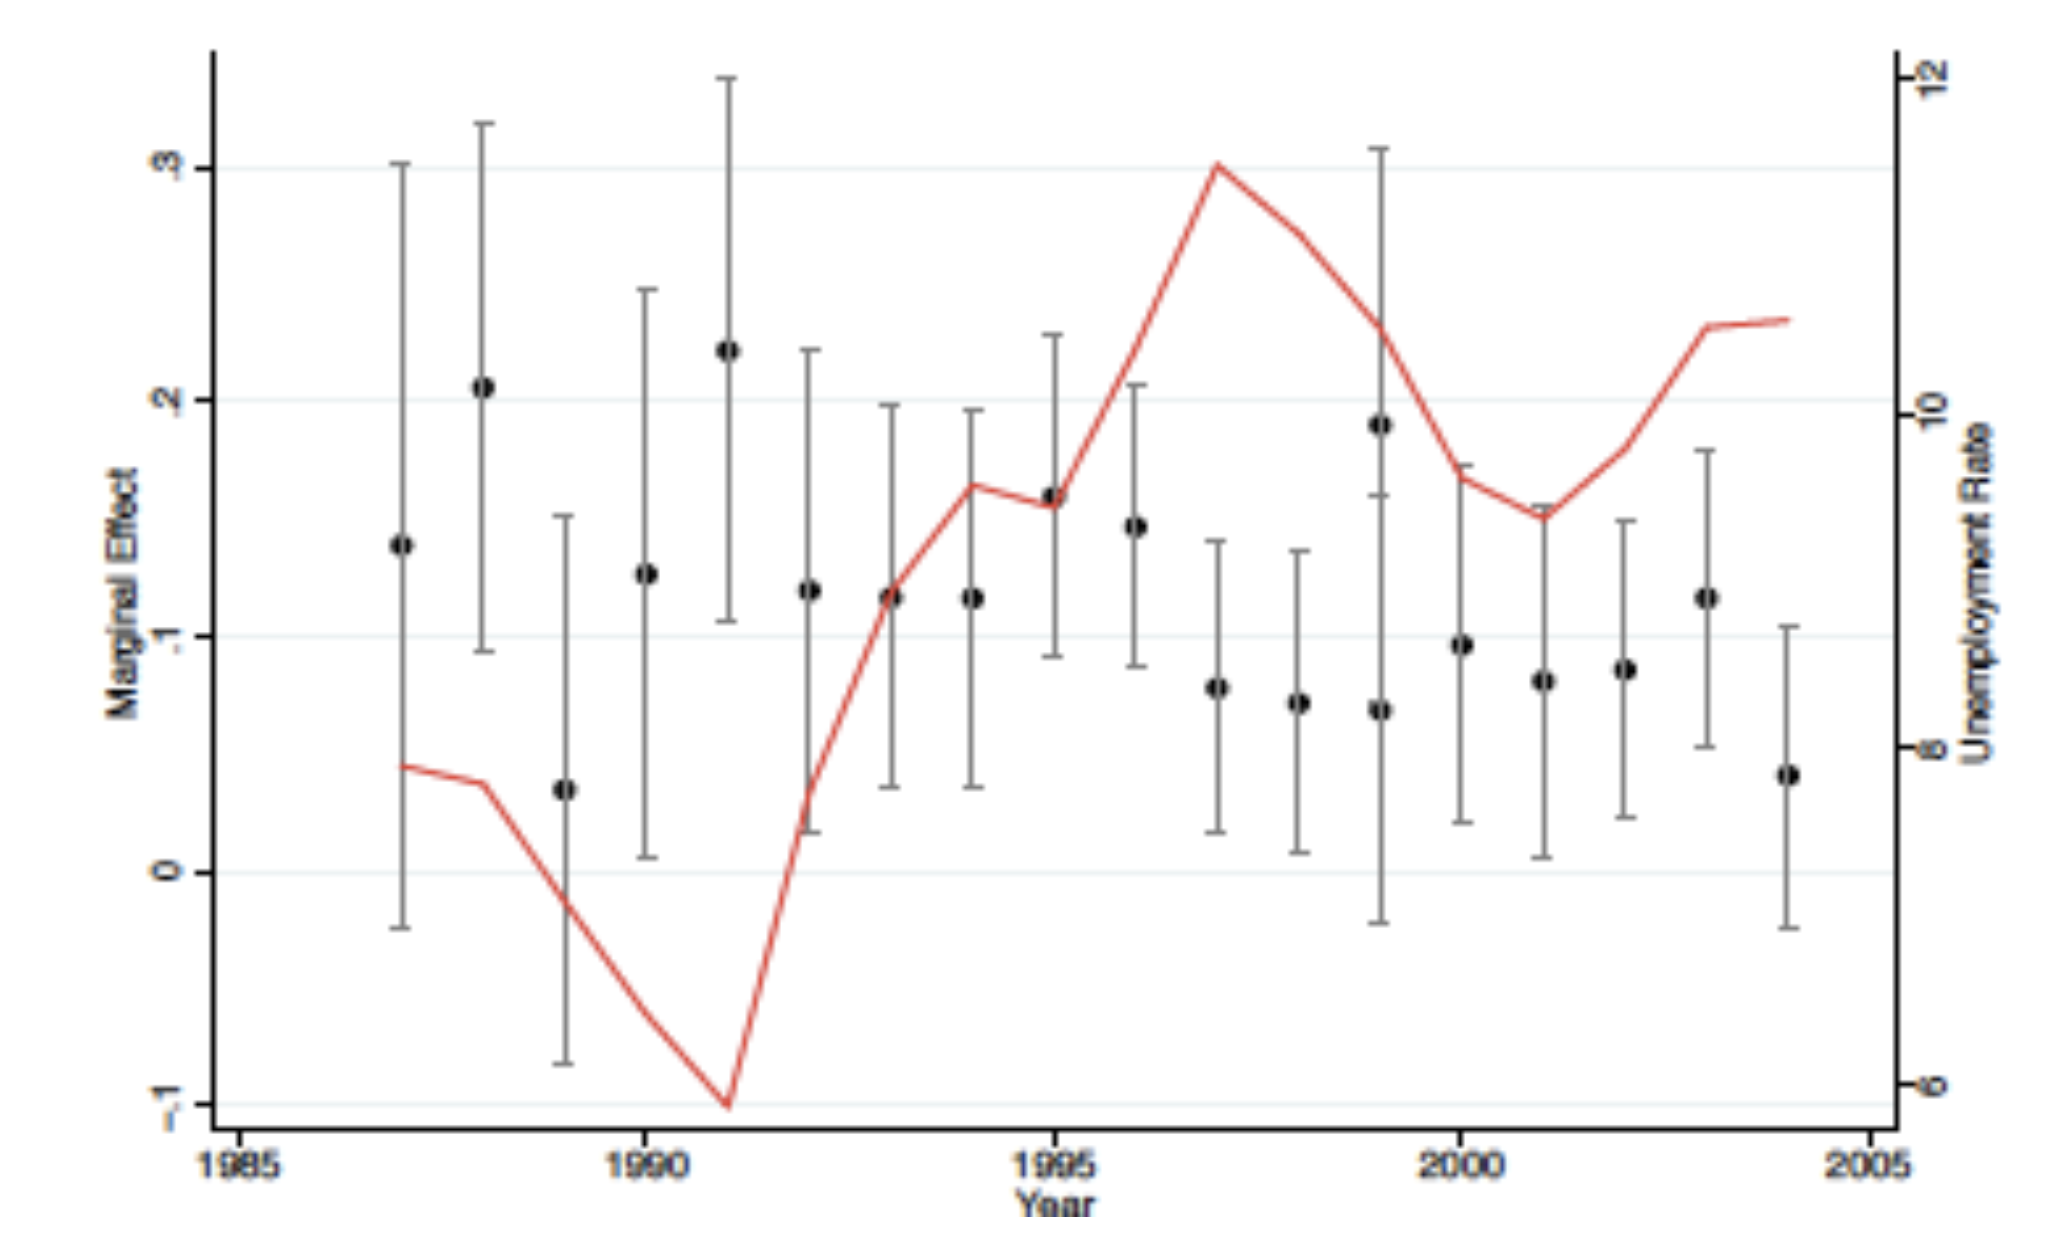
\includegraphics[width=4in]{images/ch1/Schmieder.png}
            \caption{Red line: unemployment rate; Marginal effect: shows $\frac{dp}{db}$}
        \end{figure}
        
    \subsection{Consumption Smoothing and the Business Cycle}
    Kroft and Notowigdio (2015) replicate and extend works by Gruber (1997). They estimate how the effect of UI on the consumption drop upon unemployment varies with the state unemployment rate in the previous year. They do not find evidence for larger or smaller drop in consumption when unemployment is higher. Thus, we can conclude that the \empha{value of consumption smoothing does not vary with the business cycle}.
    
    \subsection{Counter-cyclical UI Benefits}
    As discussed in the two subsections above: during a recession, moral hazard costs decrease while insurance values do not change. Therefore, it is \empha{optimal to implement a counter-cyclical UI benefit scheme}: benefits should be larger in recessions and lower in booms.
    
\section{Extension: Match Quality and Long-term Effects}
    We ignored another potential benefit of UI schemes in our simple model above: \emphb{improvements in match quality}. When people become unemployed and face the pressure of purchasing necessities, they may be forced to take worse jobs. For example, an experienced engineer may have no choice but to work in McDonald's. Provision of UI benefits may alleviate such mismatching.
    
    On the other hand, if UI benefits induce people to stay unemployed longer, there may be \emphb{skill deprecation}: an unemployed individual may lose his/her social skills and self-esteem.
    
    Which of these dominates is an empirical question:
    \begin{itemize}
        \item Card, Chetty, and Weber (2007) exploit the same discontinuity in Austria to examine the effect on subsequent wages or on subsequent job tenure, and found no significant improvement
        \item Schmieder et al. (2015) use RDD to examine the effect of extending UI eligibility from 12 months to 18 months at age 42 in Germany. They found non-employment duration increases by 1 months while re-employment wage decrease by 3\%, supporting skill deprecation.
        \item Nekoei and Weber (2015) use RDD to examine the effect of extending UI eligibility from 7.5 months to 9.5 months at age 42 in Austria. They find that non-employment duration increases by 3 days, and they also find positive effects on wages, suggesting that UI benefits improve matching quality.
    \end{itemize}
    
    All in all, empirical results are contradictory. In reality, it is \empha{very likely that both match quality improvement and skill depreciation exist}. The overall effect depends on which one dominates.
    \chapter{Minimum Wage}

\fancyhead[L]{ECON0024}
\fancyhead[C]{Ch.2 Minimum Wage}
\fancyhead[R]{Xiaotian Tian}
\fancyfoot[L]{\hyperlink{tableofcontents}{Back to Table of Contents}}
\fancyfoot[R]{Xiaotian Tian}

\section{$\star$ Neoclassical Model (Price Theory)}

    \subsection{Firm's Problem and Equilibrium}
        Firms maximise their profits by choosing the level of employment $L_j$ and taking market-level wage $w$ as given:
        $$\max_{L_j} pf(L_j) - wL_j$$
        The FOC is:
        $$\color{red} \underbrace{pf'(L_j)}_{\text{Marginal\ Revenue\ Product}} = \underbrace{w}_{\text{Marginal Cost}}$$
        Therefore, the \emphb{equilibrium employment} is:
        $$L_j^*=f'^{-1}\left(\frac{w}{p}\right)$$
        \begin{figure}[H]
            \centering
            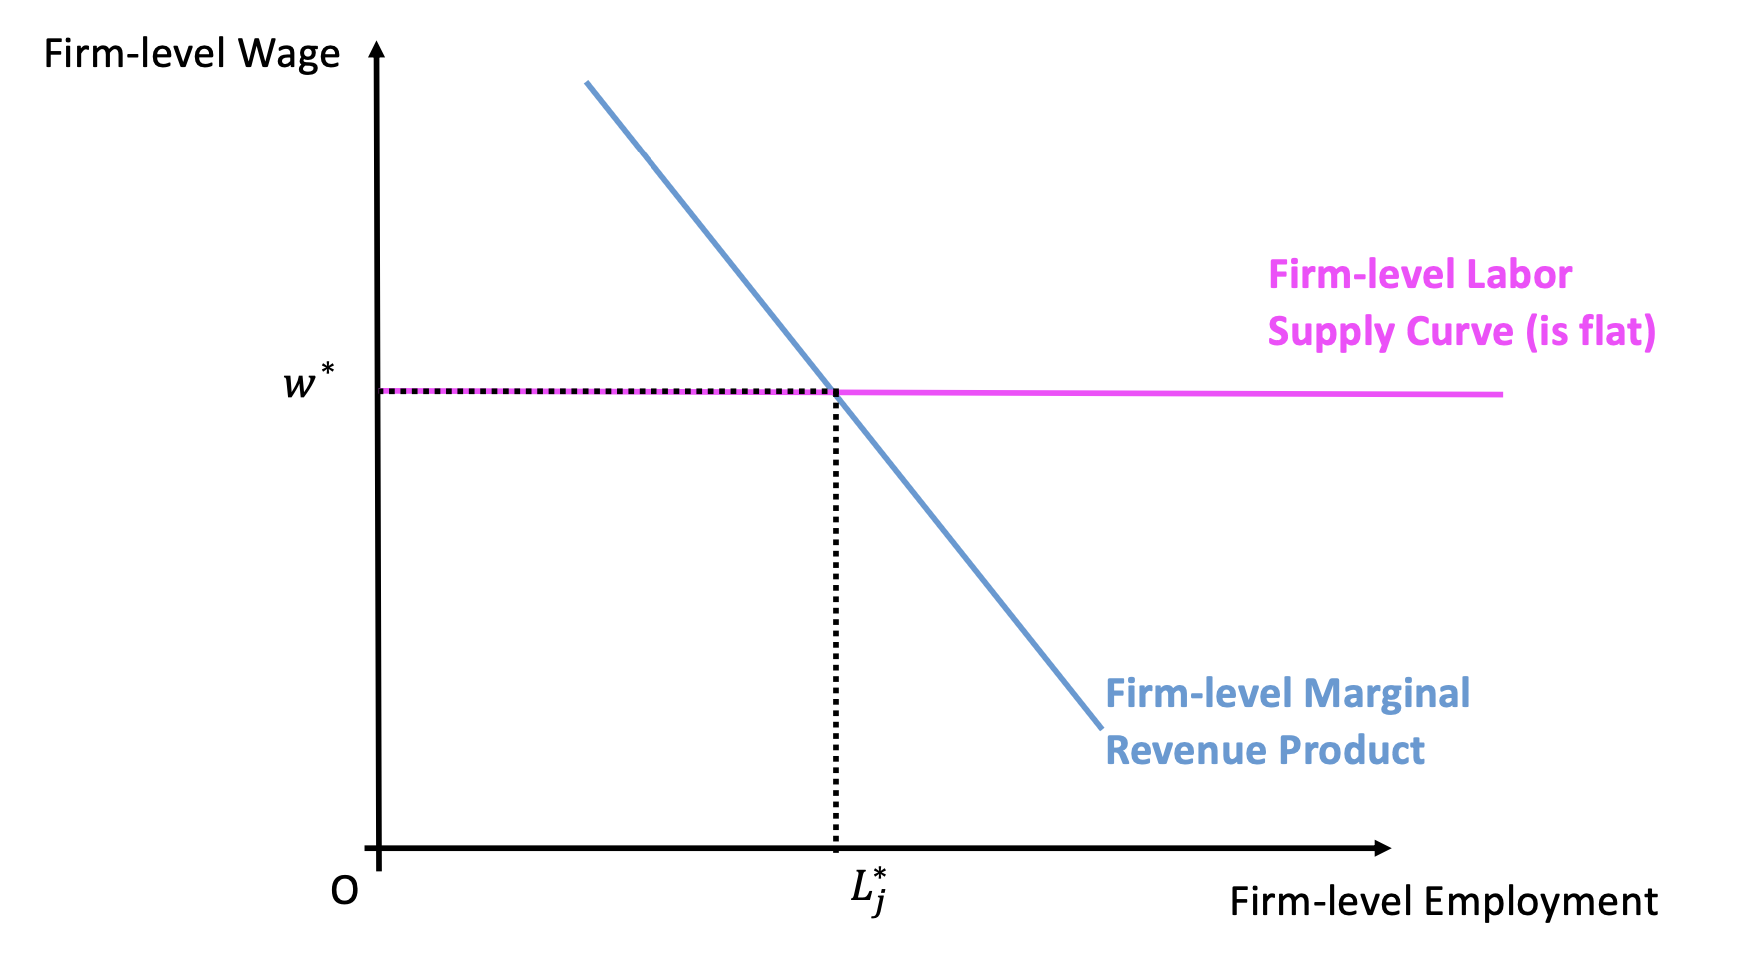
\includegraphics[width=4in]{images/ch2/neoclassical_1.png}
            \caption{Neoclassical Model: Firm's Problem}
        \end{figure}
        \begin{figure}[H]
            \centering
            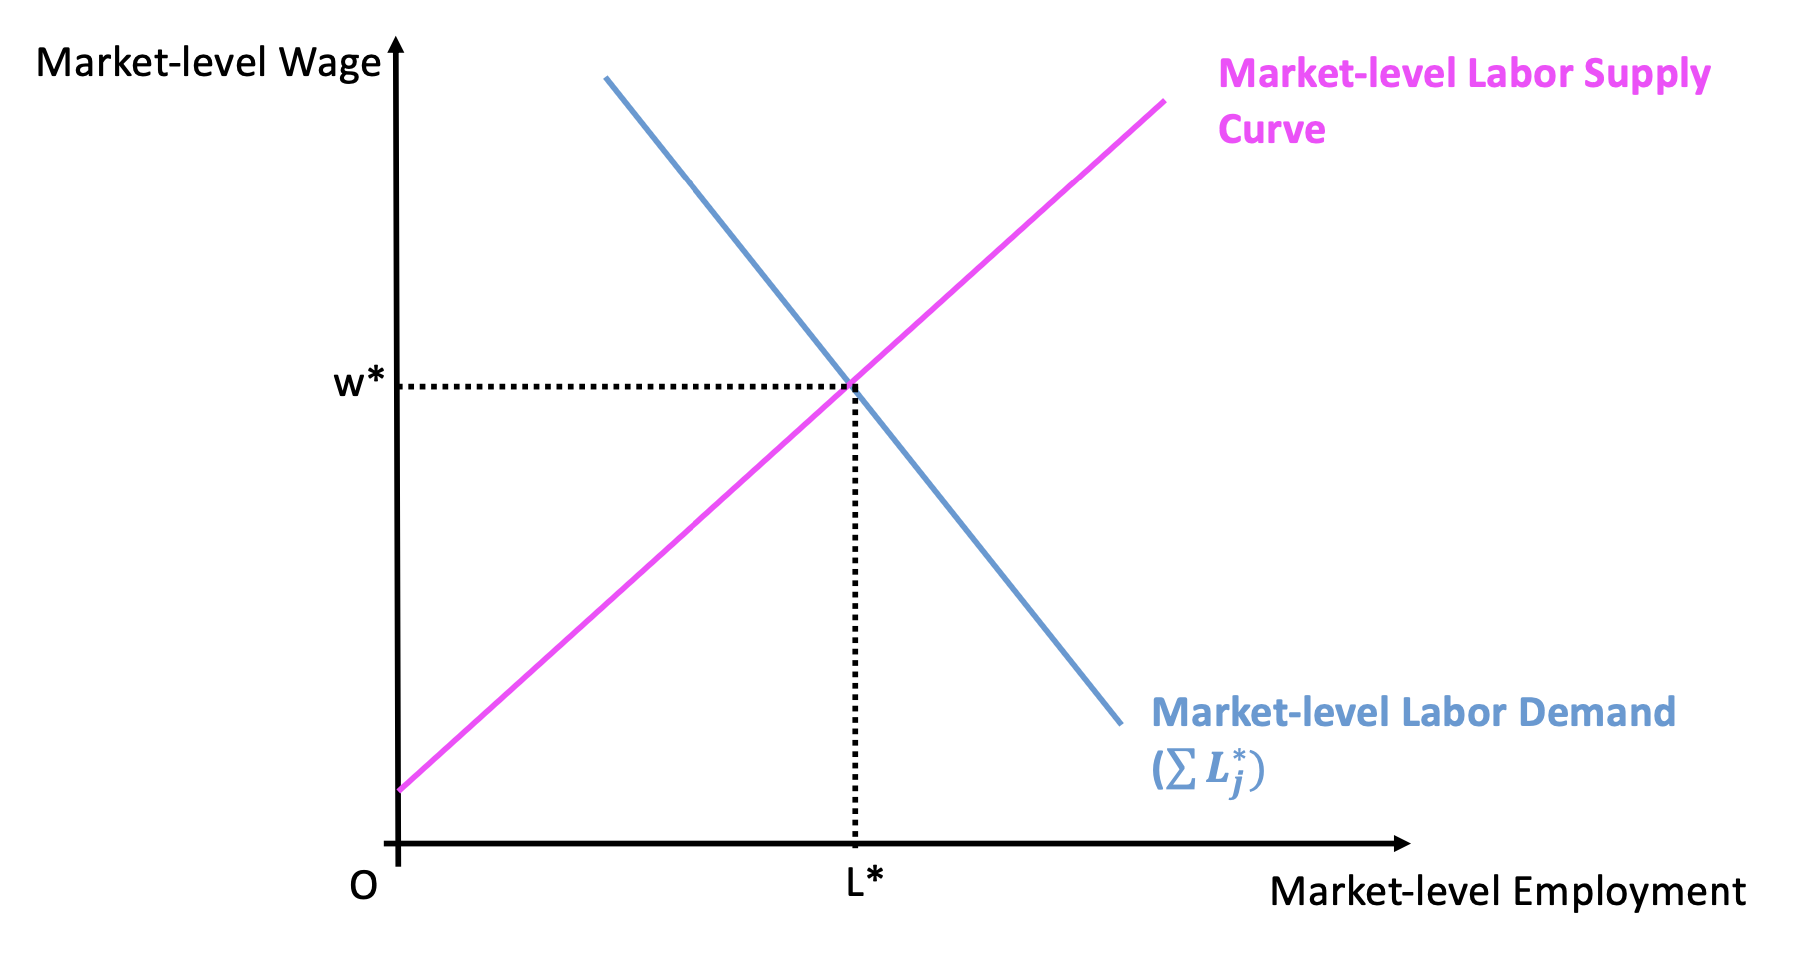
\includegraphics[width=4in]{images/ch2/neoclassical_2.png}
            \caption{Neoclassical Model: Market Equilibrium}
        \end{figure}
        
    \subsection{Effect of Minimal Wage}
        At firm's level, \empha{a minimal wage above equilibrium induces decrease in employment}:
        \begin{figure}[H]
            \centering
            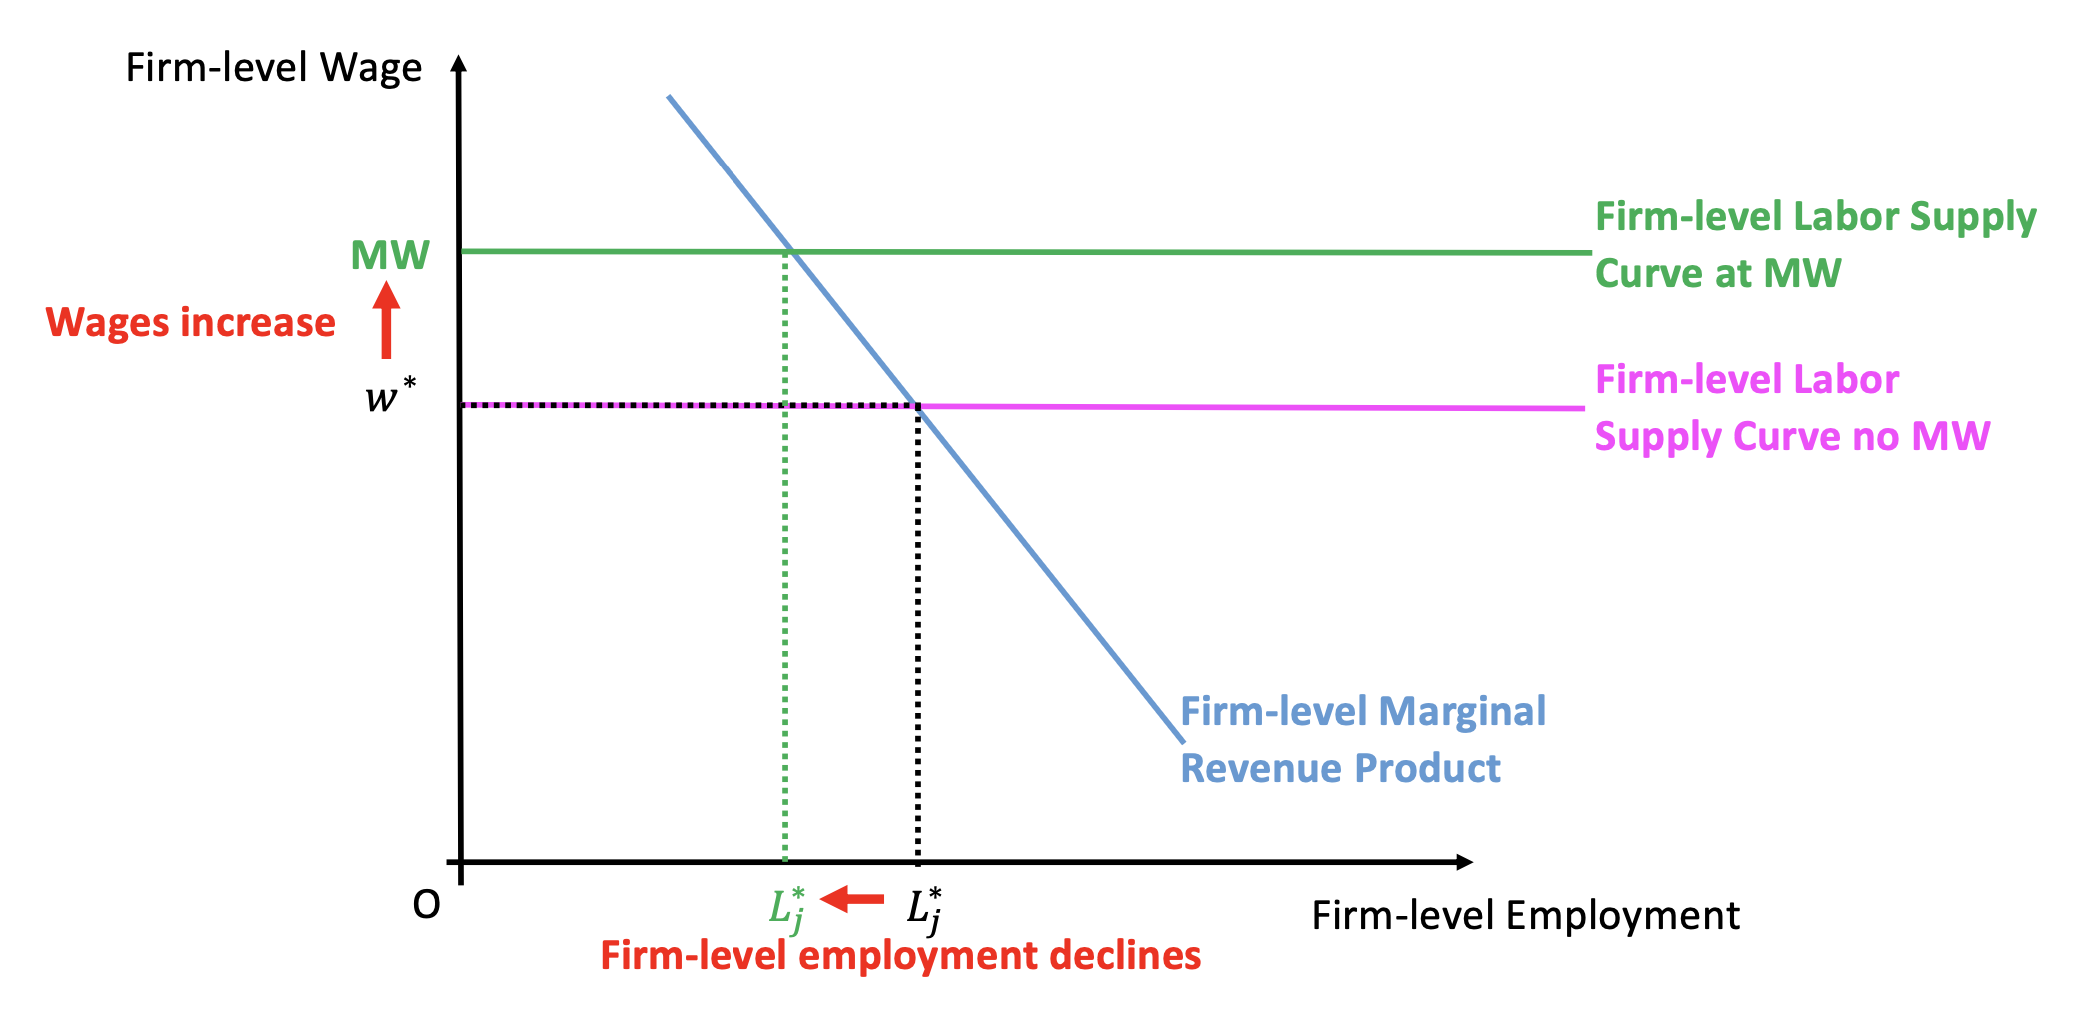
\includegraphics[width=4in]{images/ch2/neoclassical_3.png}
            \caption{Minimal Wage: Firm's Response}
        \end{figure}
        At market level, this causes a welfare loss:
        \begin{figure}[H]
            \centering
            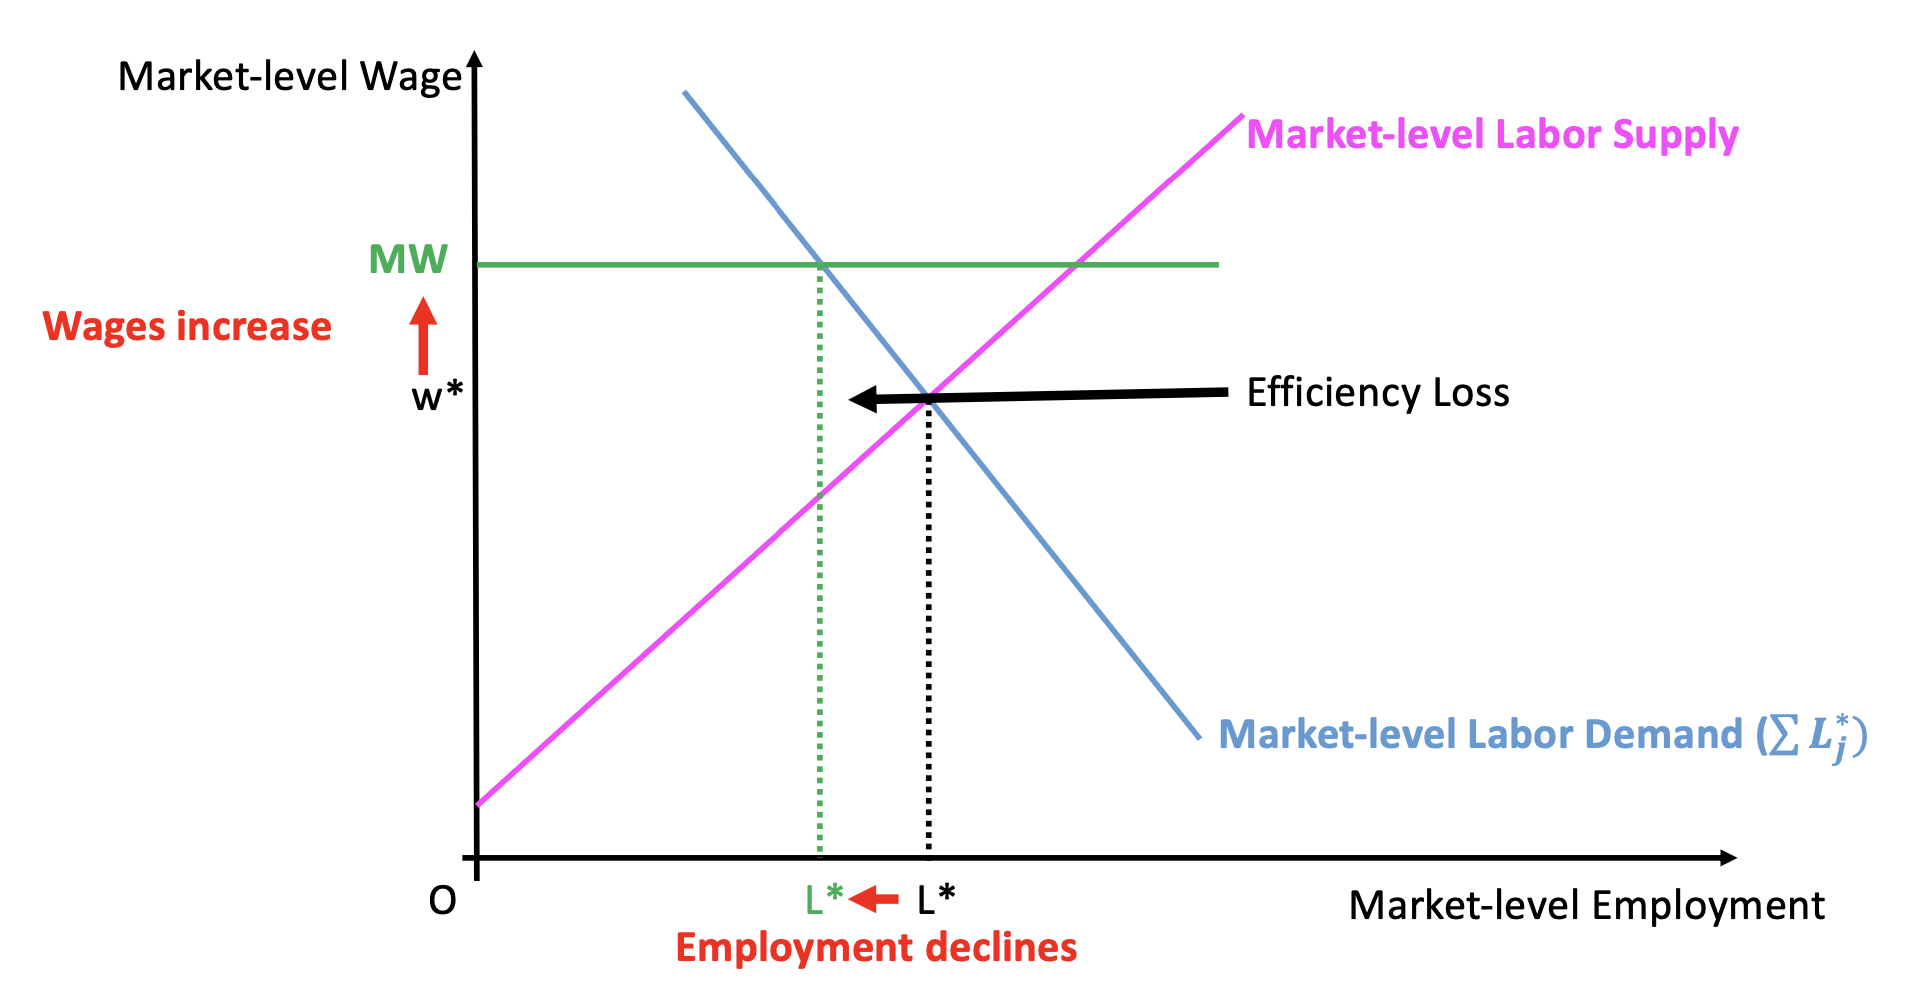
\includegraphics[width=4in]{images/ch2/neoclassical_4.png}
            \caption{Minimal Wage: Market Equilibrium}
        \end{figure}
    
    \subsection{Debate over the Neoclassical Model and the Consensus}
    
        \subsubsection{George Stigler (1946): Price Theory}
            \begin{itemize}
                \item There is no free lunch
                \item Minimum wage decreaes employment and leads to efficiency loss
                \item (This is a testable prediction)
            \end{itemize}
            
        \subsubsection{Richard Lester (1947): Common Sense Approach}
          \begin{itemize}
              \item Abandoned the model and looked at data instead
              \item Ask managers about what determines employment
              \item Most important factor mentioned in responses: demand of output
              \item Less than 20\% reported labour cost as the most important factor
              \item Conclusion: (small) increase in labour cost will have a limited effect on employment
          \end{itemize}
          
        \subsubsection{The Consensus: Milton Friedman (1953): “Essays in Positive Economics”}
            \begin{itemize}
                \item Assumptions can be unrealistic and simplifying
                \item A good model focuses on the most important mechanisms, instead of discussing all irrelevant ingredients
                \item A good model can explain and predict what happens if circumstances change
                \item Evidence produced over the 60-80s supports declining employment
                \item \textbf{Consensus}: Chicago-style approach/price theory captures what happens in response to a minimum wage
            \end{itemize}
    
\section{Consensus Breaks: Modern Empirical Evidences}

    \subsection{Card and Krueger (1994, 1995) and the “Credibility Revolution”}
    
        \subsubsection{Card and Krueger (1994, 1995)}
            Card and Krueger (1994, 1995) studied the impact of an increasing minimum wage in New Jersey with a Difference-in-Difference approach. Their control group is Pennsylvania where there was no minimum wage hike. Their results showed that the increase in minimum wage \empha{increased both wages and employment} in New Jersey. This contradicted the neoclassical model.
            \begin{itemize}
                \item Their DiD design:
                $$\Delta E_i = \alpha + \beta 'X_i + \gamma NJ_i + \epsilon_i$$
                where $X_i$ controls for store characteristics and $NJ_i$ is a dummy takes value 1 for New Jersey.
                \item Their Exposure design:
                $$\Delta E_i = \Tilde{\alpha} +\Tilde{\beta} 'X_i +\Tilde{\gamma} GAP_i + \Tilde{\epsilon}_i$$
                where $GAP_i = NJ_i \times \max \left\{\frac{5.05 - W_{1,i}}{W_{1,i}},0\right\}$ accounts for the wage increase due to the policy.
            \end{itemize}
            Results:
            \begin{figure}[H]
                \centering
                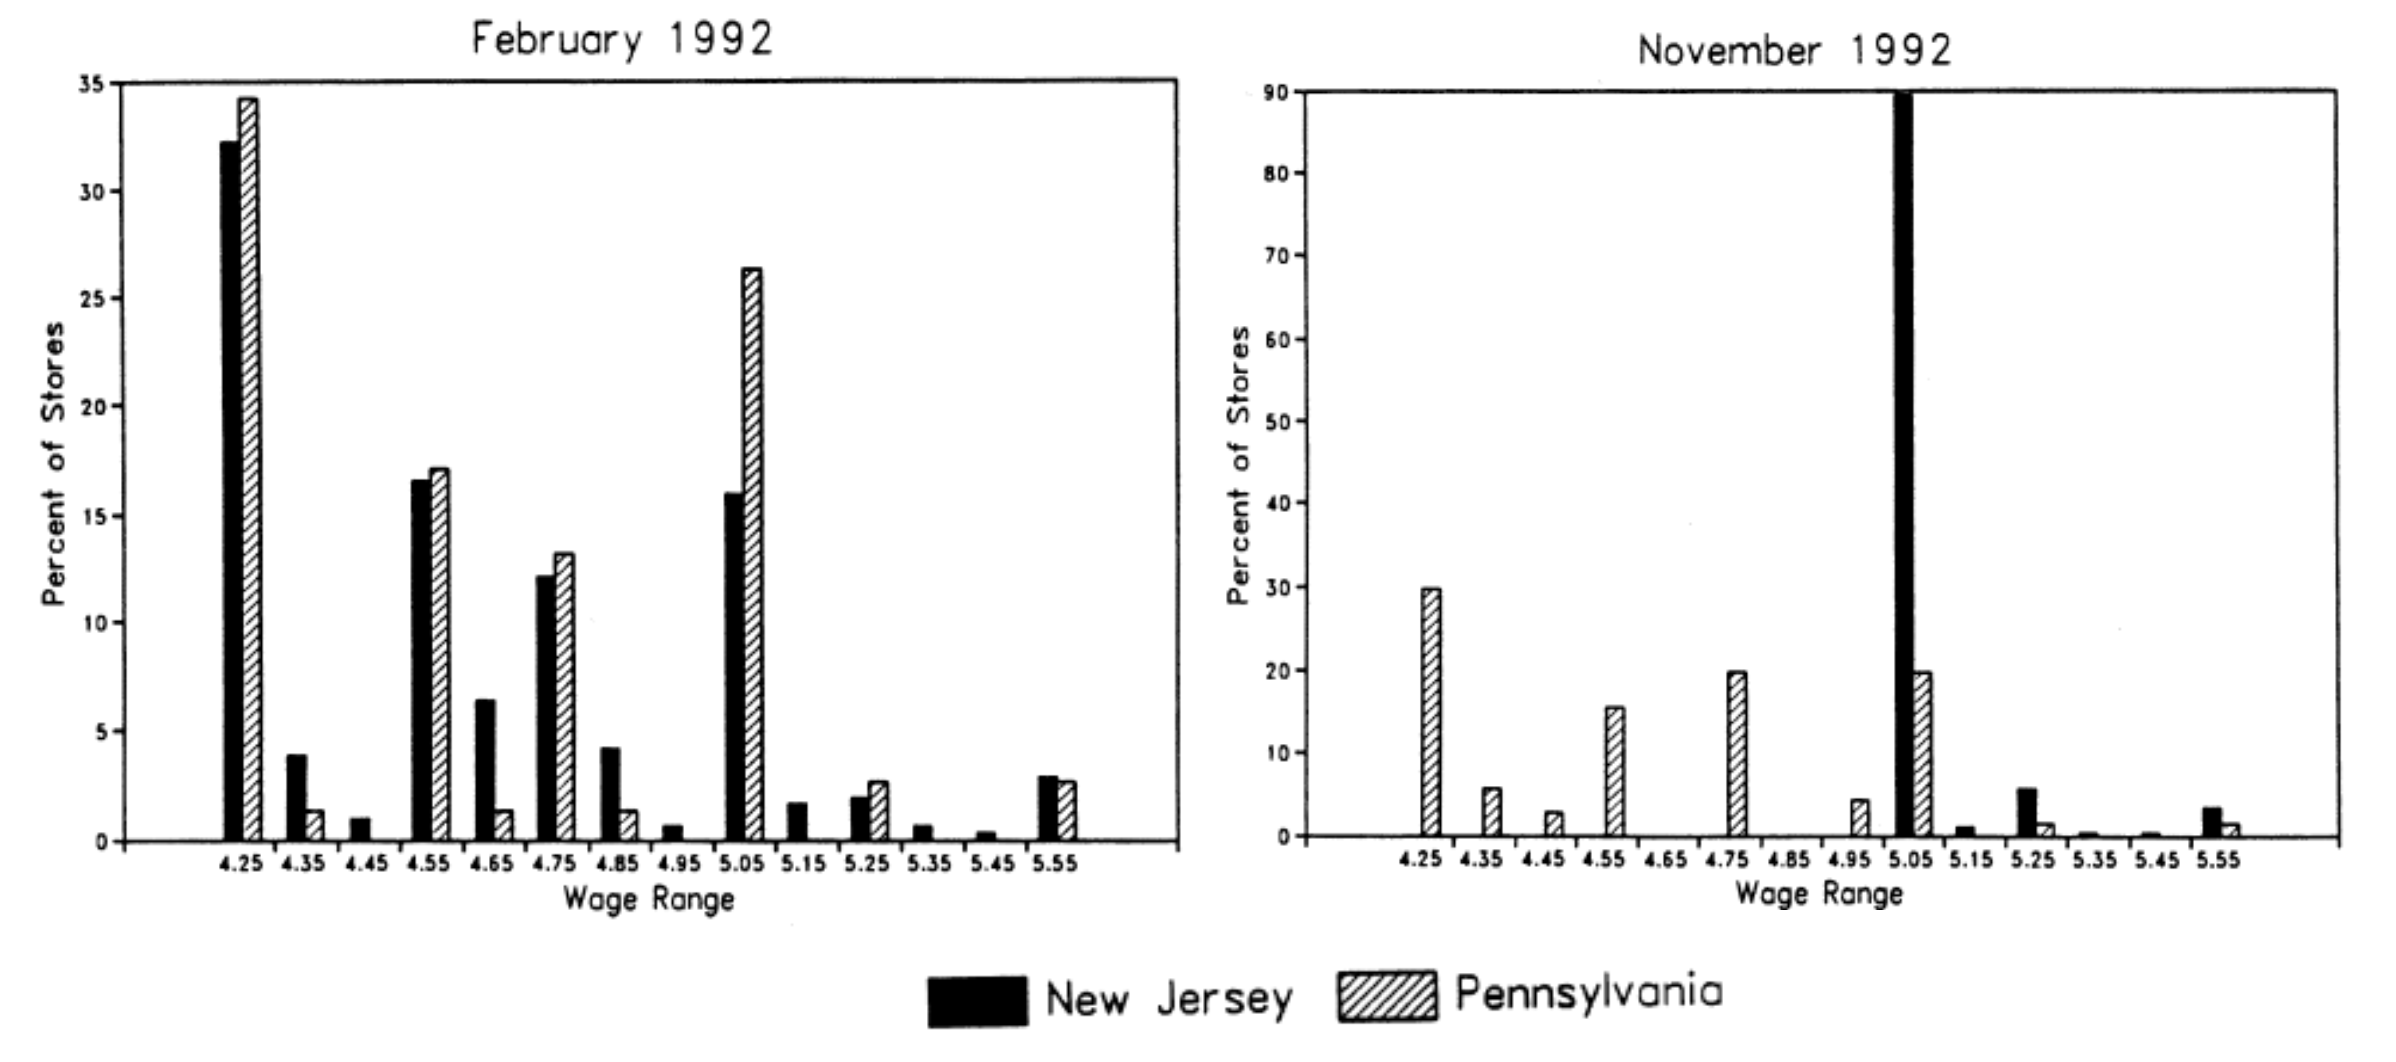
\includegraphics[width=5in]{images/ch2/New Jersey.png}
                \caption{Wage Distributions}
            \end{figure}
            \begin{figure}[H]
                \centering
                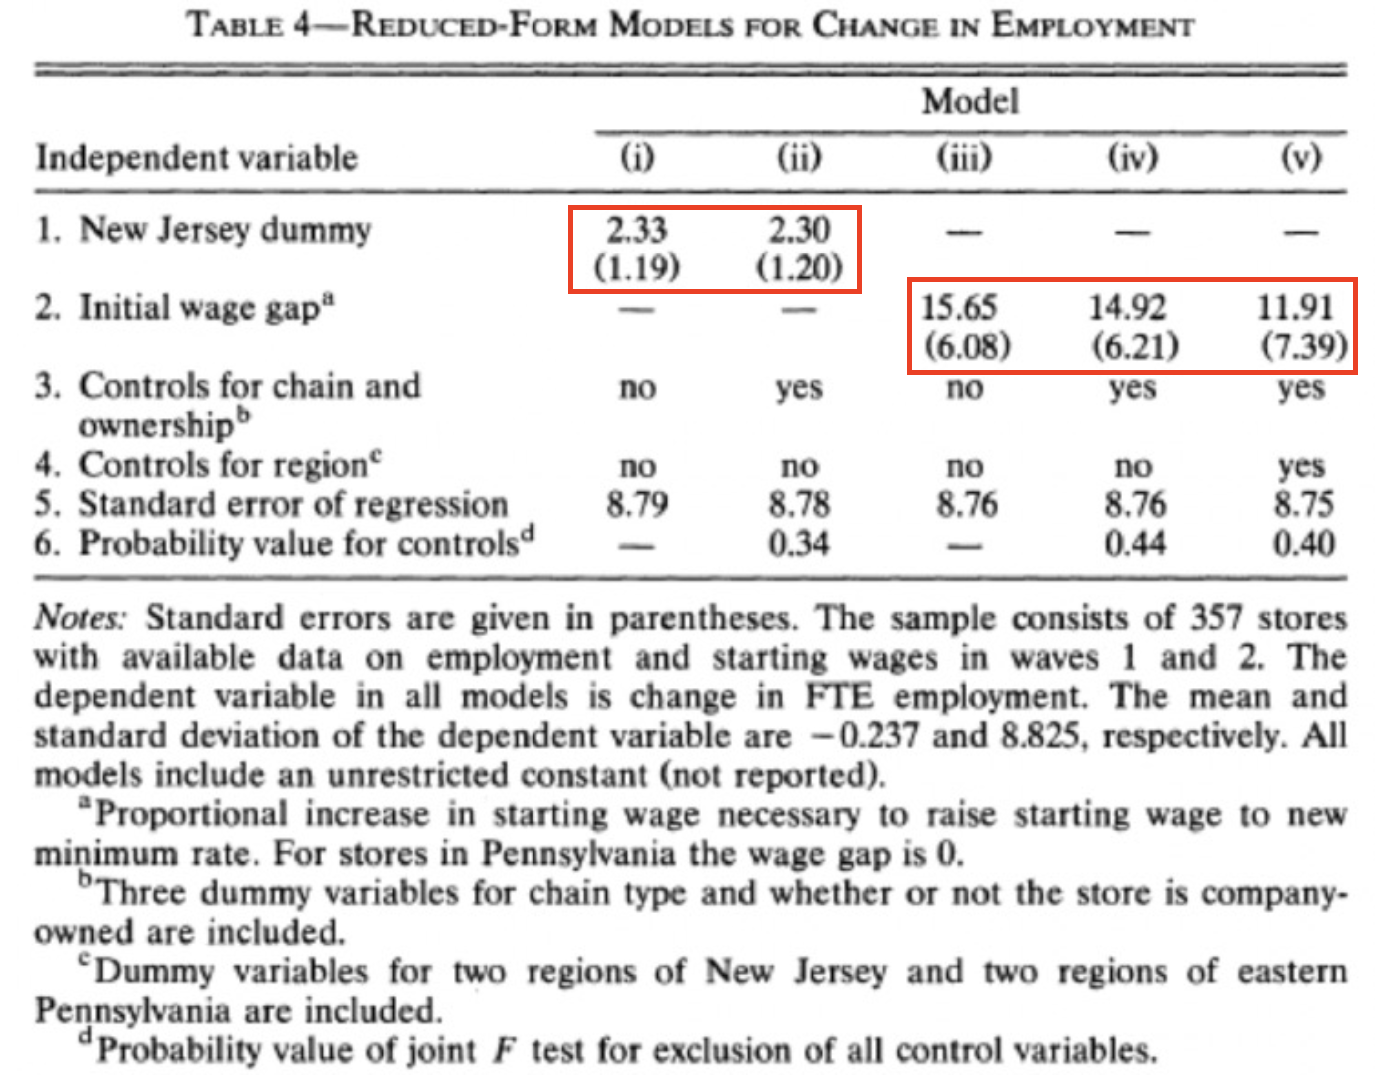
\includegraphics[width=4in]{images/ch2/New_Jersey 2.png}
                \caption{1st Row: DiD; 2nd Row: Exposure Design}
            \end{figure}
            Their results provided clear evidence that the increase in minimum wages in New Jersey caused an increase in both wages and employment.
            
        \subsubsection{A Lesson Learnt for Economists}
            \begin{itemize}
                \item Economic models are important as they can capture the most important mechanisms at play
                \item Simplicity is value, but we should not be dogmatic about our models
                \item We need “credible” research designs, that could be used to reject or accept the key predictions of our models
                \item Alan Krueger (2018): “The idea of turning economics into a true empirical science, where core theoriescan be rejected, is a BIG, revolutionary idea.”
            \end{itemize}
    
    \subsection{New Mimimum Wage Research}
        New minimum wage research shifted the focus from theory to \emphb{"reduced form"} empirical evidence on employment and wages, investigating the impact of minimum wages directly.
        
        The U.S. has been a fertile ground due to state-level variations that can be exploited:
        \begin{itemize}
            \item Two-way Fixed Effects estimation (e.g. Neumark and Wascher, 1993)
            \item Usage of administrative data (e.g. Card and Krueger, 2000)
            \item Border-discontinuity design (e.g. Dube, Lester and Reich, 2010)
        \end{itemize}
        
        On the other hand, most of the evidence focuses on specific demographic groups (e.g. teens) or sectors (e.g. restaurants). It could be possible that minimum wages increase employment in some sectors but decrease it in others.
        
    \subsection{Frequency Distribution Based Approach}
        \subsubsection{Idea}
        Cengiz et al. (2019) develop a novel method to assess the overall employment change using changes in distribution:
        \begin{figure}[H]
            \centering
            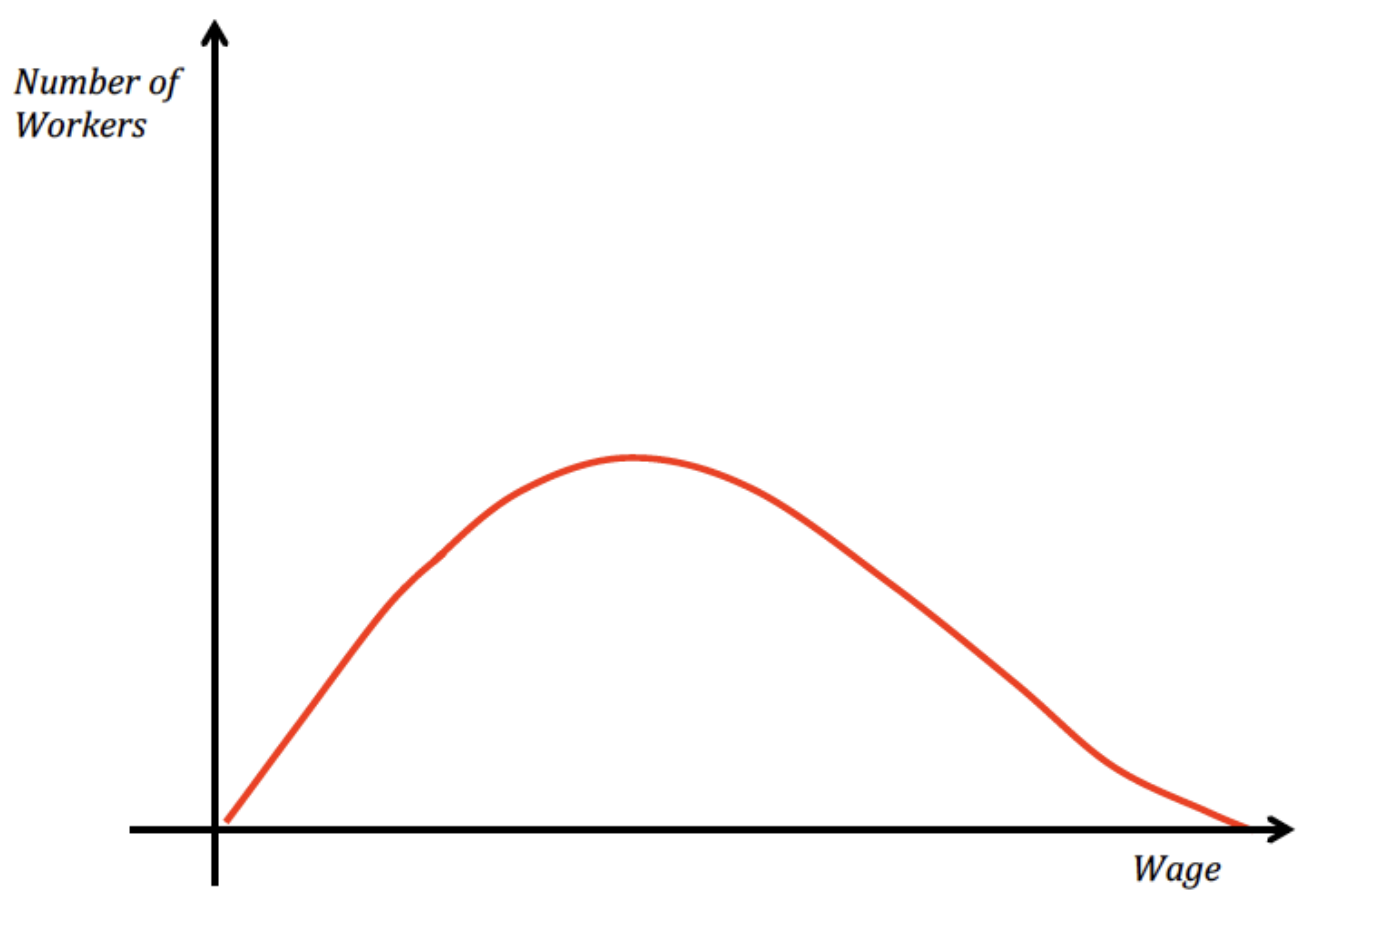
\includegraphics[width=4in]{images/ch2/Freq_approach_1.png}
            \caption{Distribution of Employment before Policy Change}
        \end{figure}
        After an increase in the minimum wage, jobs with wages below the threshold will disappear and new jobs with wages higher than the threshold will be generated. The net effect on employment is illustrated below:
        \begin{figure}[H]
            \centering
            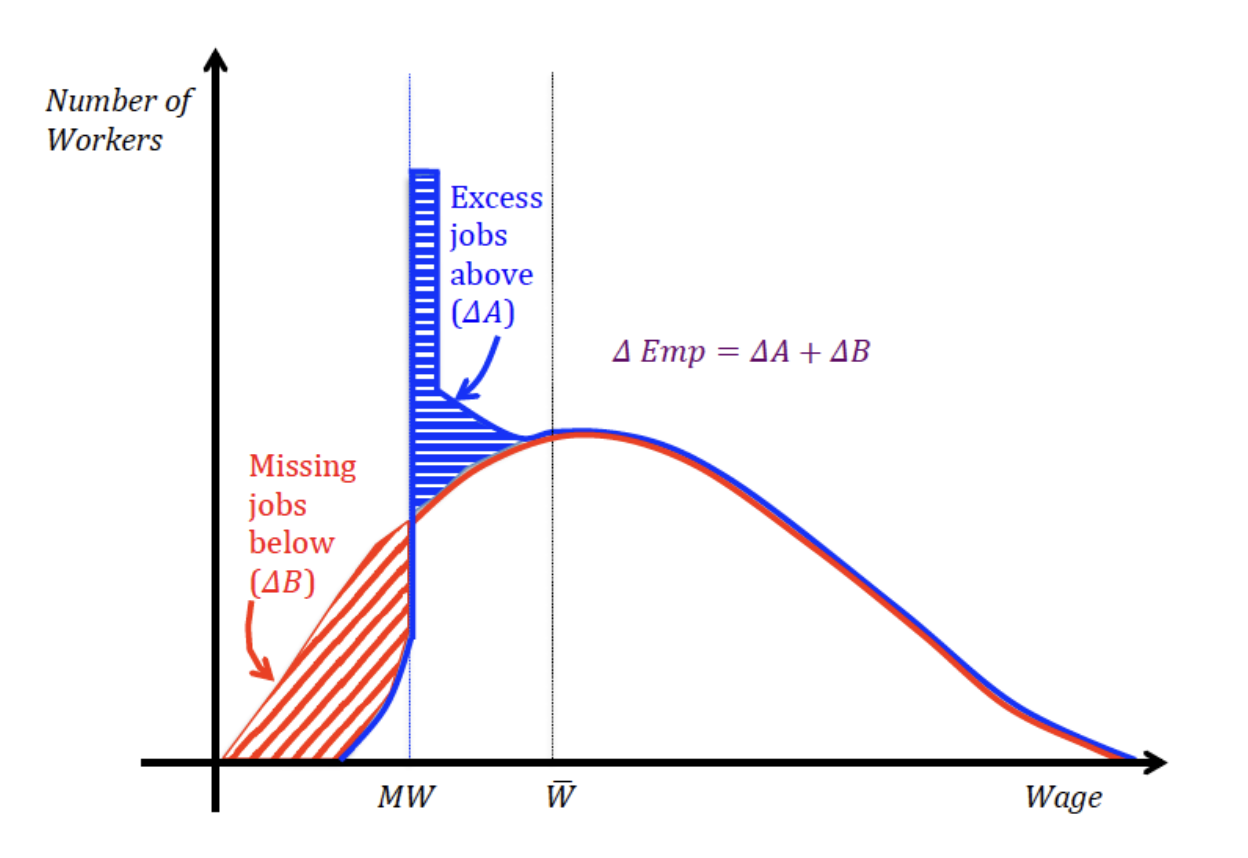
\includegraphics[width=4in]{images/ch2/Freq_approach_2.png}
            \caption{Distribution of Employment after Policy Change}
            \label{fig:freq_approach}
        \end{figure}
        The key empirical challenge of this method is to get counterfactual wage distribution. The solution is to use a DiD idea.
        
        During 1999-2000, Washington State raised its minimum wage from \$7.51 to \$9.18, and WA has administrative data on hourly wages. We divide the distribution by wage bins, and calculate the counterfactual by creating a synthetic control group from a number of states.

        With this method, Cengiz et al. obtained both actual and counterfactual employment distributions:
        \begin{figure}[H]
            \centering
            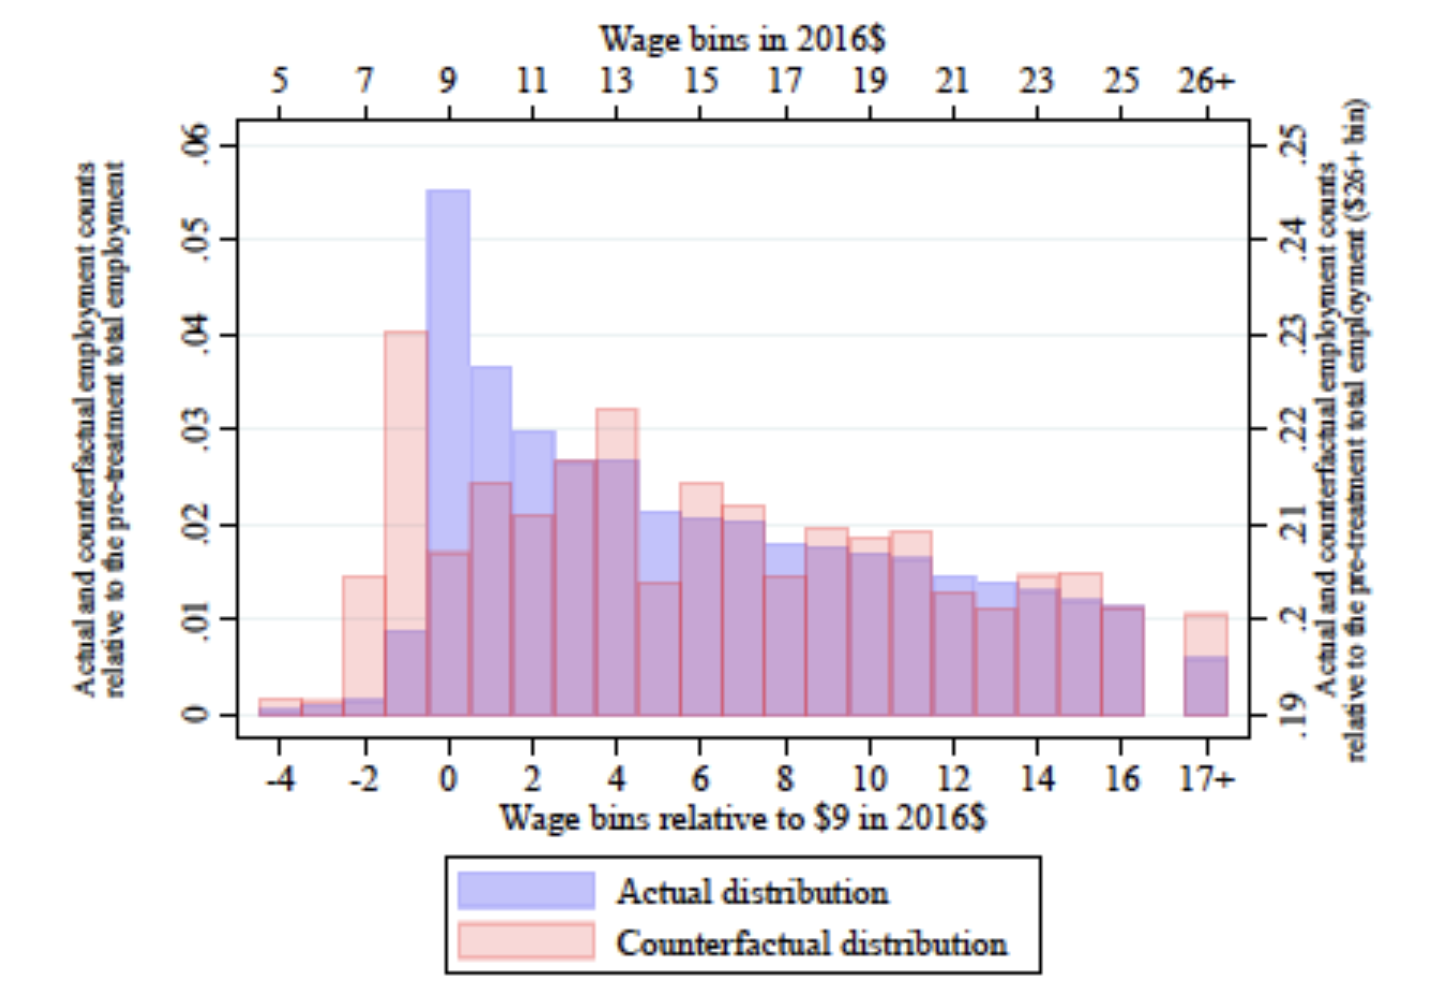
\includegraphics[width=3.5in]{images/ch2/Freq_approach_3.png}
            \caption{Actual and Counterfactual Distributions}
        \end{figure}
        Comparing the two distributions, the effect of an increase in minimum wage is retrieved. The patter of change matches Figure \ref{fig:freq_approach}, and, as shown by the red line, there is a redistribution of employment from jobs with wages below the threshold to jobs with wages above the threshold. No reduction in overall employment is observed:
        \begin{figure}[H]
            \centering
            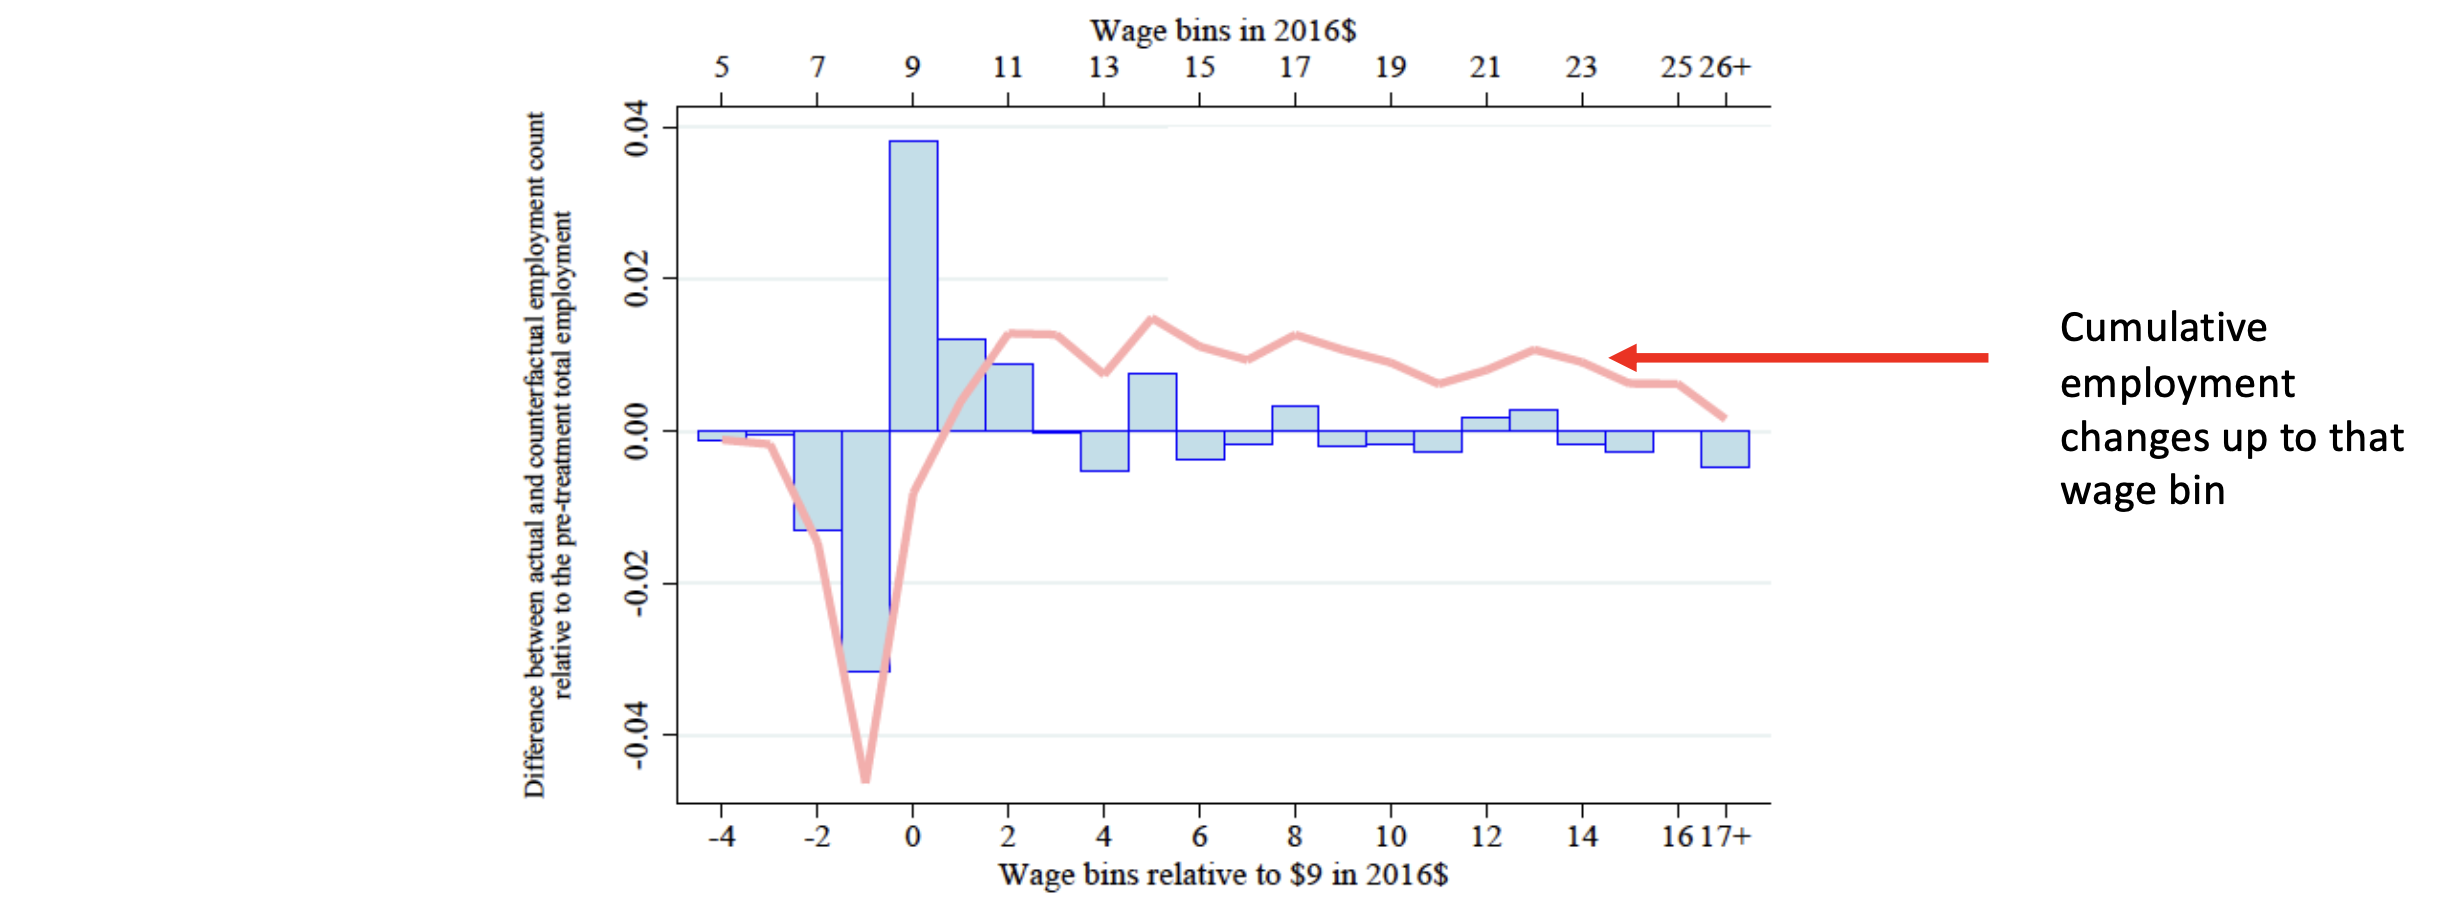
\includegraphics[width=6.5in]{images/ch2/Freq_approach_4.png}
            \caption{Treatment Effect}
        \end{figure}
        Taking heterogeneity into account, we cannot find any overall dis-employment either:
        \begin{itemize}
            \item No evidence that dis-employment effects are more prominent for larger changes
            \begin{figure}[H]
                \centering
                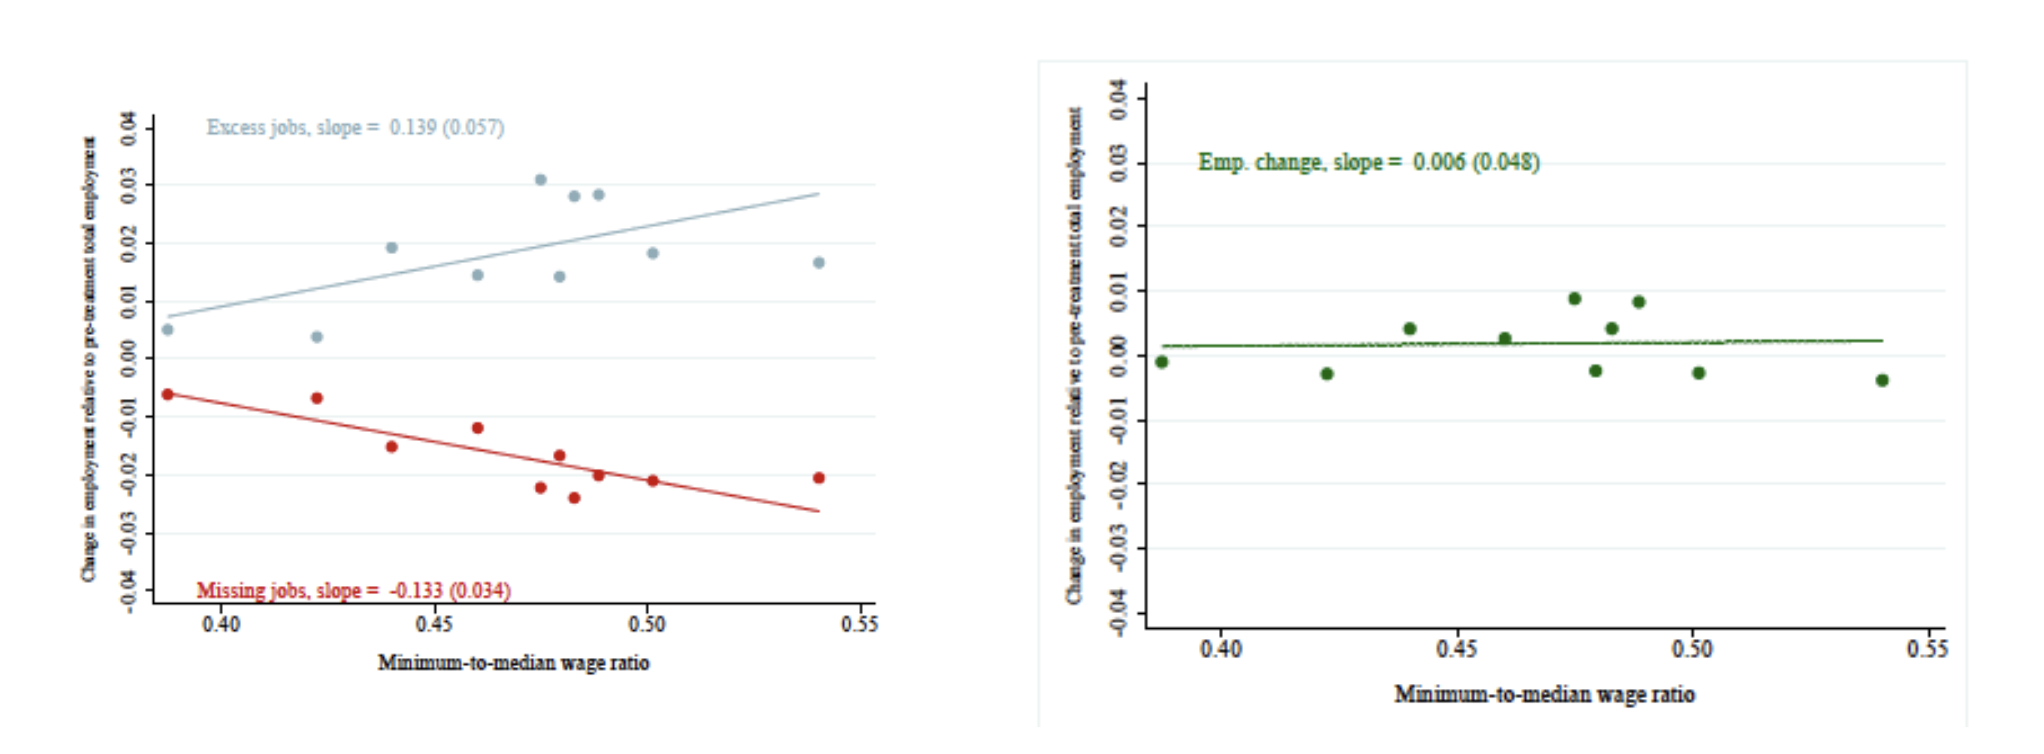
\includegraphics[width=5.5in]{images/ch2/Freq_approach_5.png}
                \caption{Heterogeneity by Magnitude of Increase}
            \end{figure}
            \item No evidence that dis-employment effects are more prominent when unemployment rate is high
            \begin{figure}[H]
                \centering
                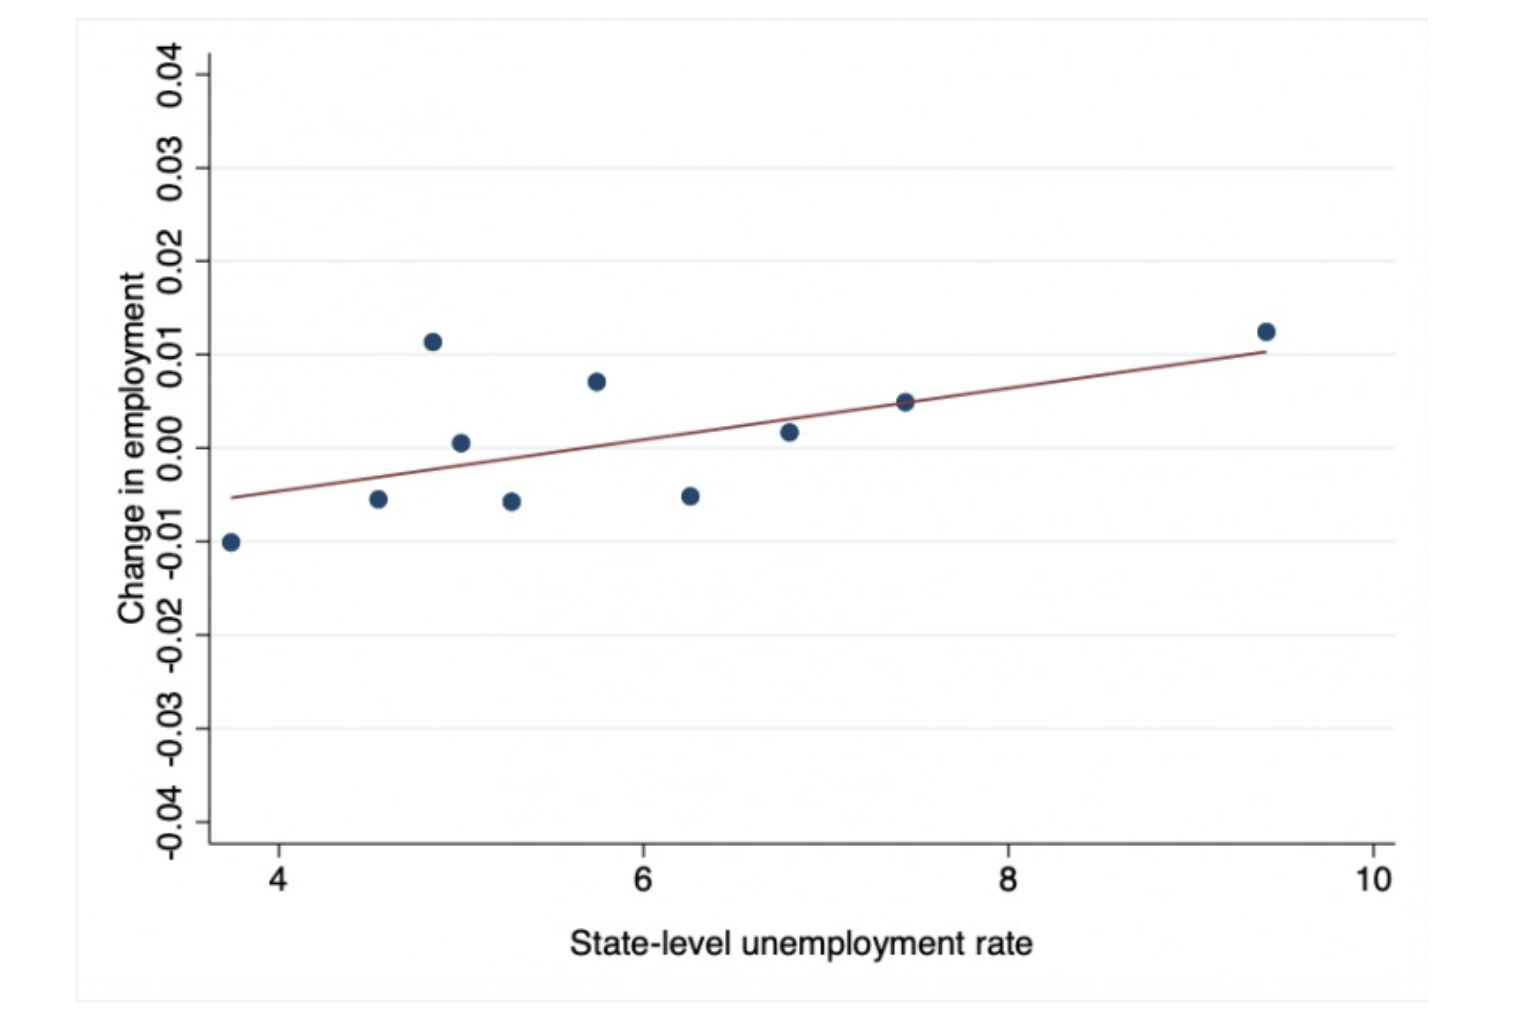
\includegraphics[width=4in]{images/ch2/Freq_approach_6.png}
                \caption{Heterogeneity by State Unemployment Level}
            \end{figure}
        \end{itemize}
        
        
\section{$\star$ Monopsonistic Model}

    \subsection{Firm's Problem and Equilibrium}
    
        \subsubsection{Assumptions}
            Empirical research presented in the previous section show no evidence that an increase in minimum wage will cause dis-employment. This indicates that assumptions we made for the standard neoclassical ``price theory'' model do not hold. In reality:
            \begin{itemize}
                \item Workspaces are differentiated (not homogeneous)
                \item Such differentiation provides each employer with some market power
                \item The labour market is a \emphb{monopsonistic market}
            \end{itemize}
            The intuition is that, because some workers want to work at a certain firm, the employer can hire them with lower wages. This creates a wedge between productivity and wages. In equilibrium, fewer workers are hired and wages are lower.
            
        \subsubsection{Firm's Optimisation Problem}
            Firms maximise their profits:
            $$\max_{L_j} pf(L_j) - w(L_j)L_j$$
            The FOC implies that:
            $$\color{red} \underbrace{pf'(L_j)}_{\text{Marginal\ Revenue\ Product}} = \underbrace{w(L_j)\left(1+\frac{1}{\eta}\right)}_{\text{Marginal\ Cost}}$$
            where $\eta$ is the \emphb{elasticity of firm-level labour supply} defined as $\eta = \frac{\partial L_j}{\partial w}\frac{w}{L_j} > 0$.
            The \emphb{equilibrium wage} in monopsonistic model is:
            $$\color{red} w^*(L_j)= \underbrace{pf'(L_j)}_{\text{Marginal\ Revenue\ Product}} \times \underbrace{\frac{1}{1+\frac{1}{\eta}}}_{\text{Mark-down}(<1)} < w^*_{Neoclassical}$$
            The equilibrium wage here is different from the marginal revenue product: firms enjoy a "\emphb{markdown}." The magnitude of such difference depends on firm-level elasticity of labour supply: if $\eta \rightarrow \infty$, we get back to the neoclassical framework.
            \begin{figure}[H]
                \centering
                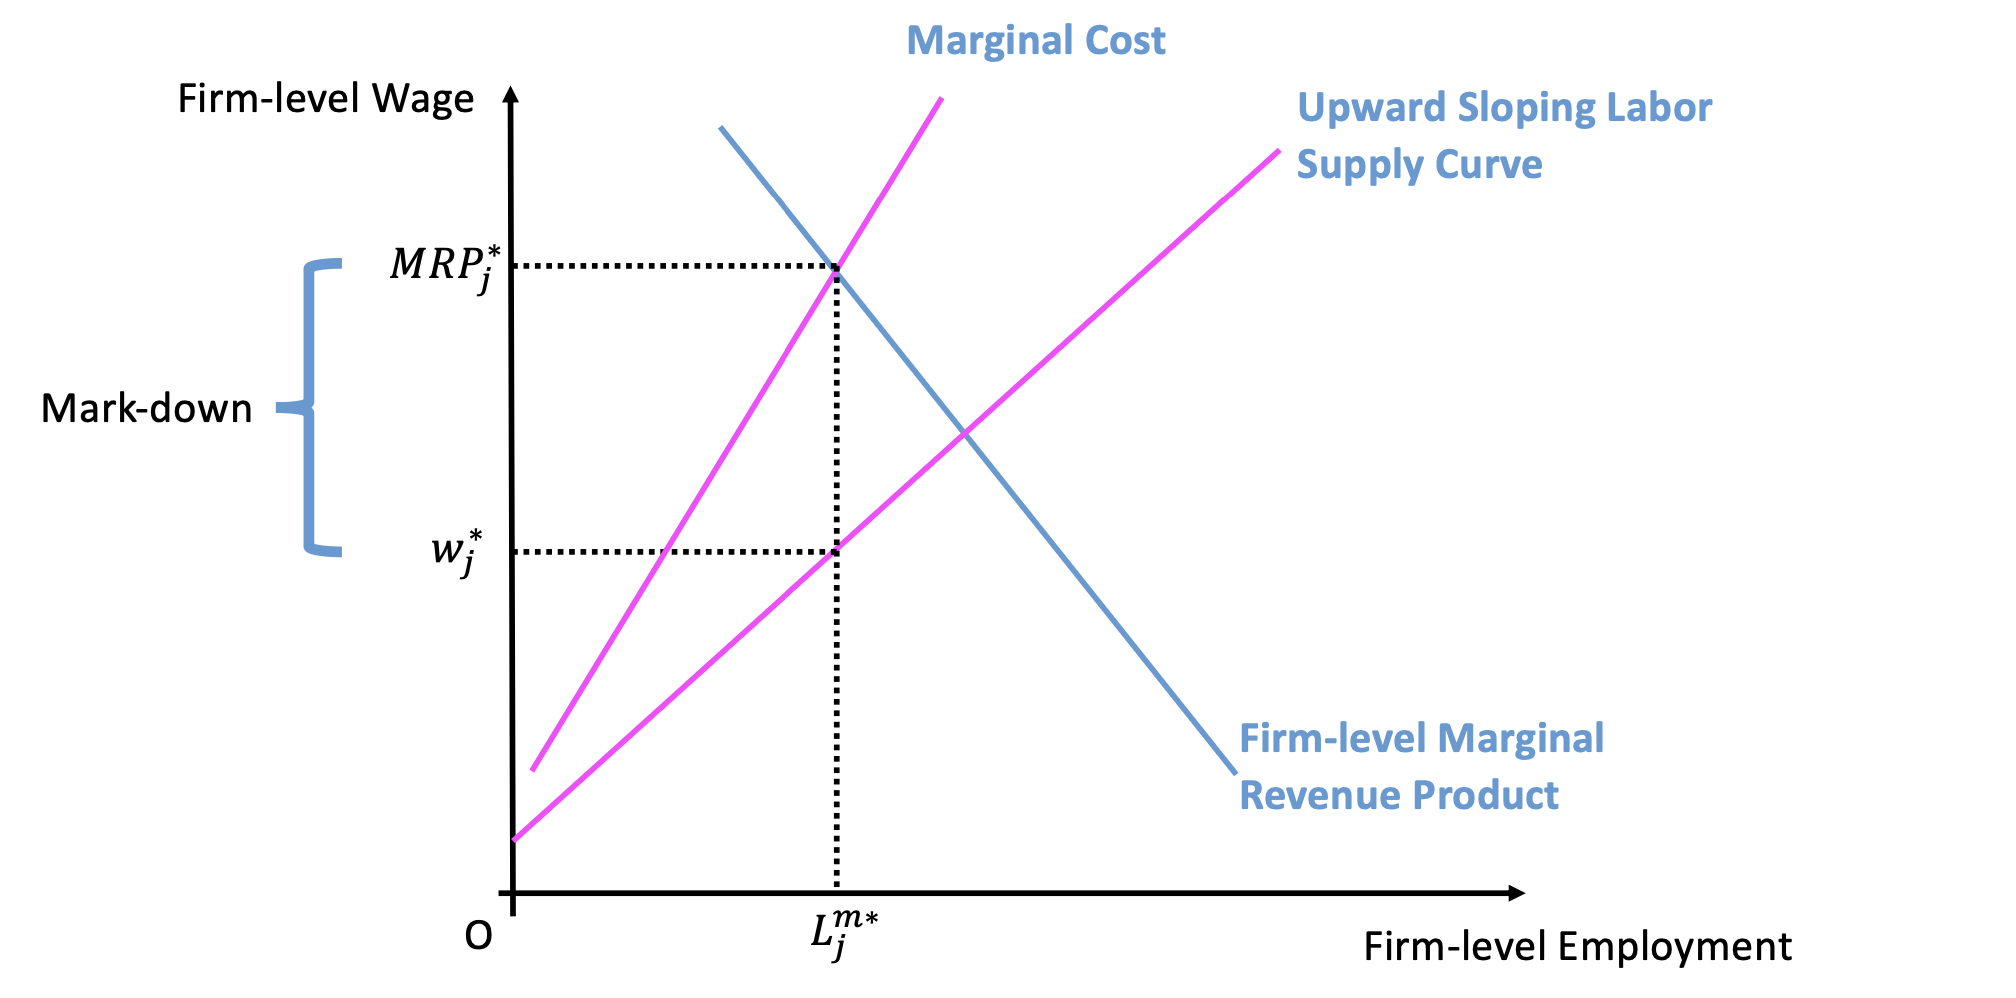
\includegraphics[width=5in]{images/ch2/Monop_LM_1.png}
                \caption{Equilibrium in a Monopsonistic Labour Market}
            \end{figure}
            
        \subsubsection{Predictions}
            Several main predictions of this monopsonistic model:
            \begin{itemize}
                \item People feel they are underpaid at their workplace relative to their true productivity – wages are “marked-down”
                \item People feel they could find a better paying workplace, but those are not ideal (they are too far from home, not nice co-workers)
                \item Workers with similar skills and ability are paid differently at different firms (there is a firm-level skill premium)
                \item Efficient firms are larger and pay more to workers with similar skills
            \end{itemize}
    
    \subsection{Effect of Minimal Wage: Reallocation}
        In this framework, a minimum wage scheme will cause:
        \begin{itemize}
            \item The least efficient firms will close
            \item The most efficient firms increase wages, the mark-down (or profit per worker) falls
            \item Though the wedge between productivity and wage falls, it is still profitable to employ workers
            \item Firms will hire more with lower mark-down
        \end{itemize}
        \begin{figure}[H]
            \centering
            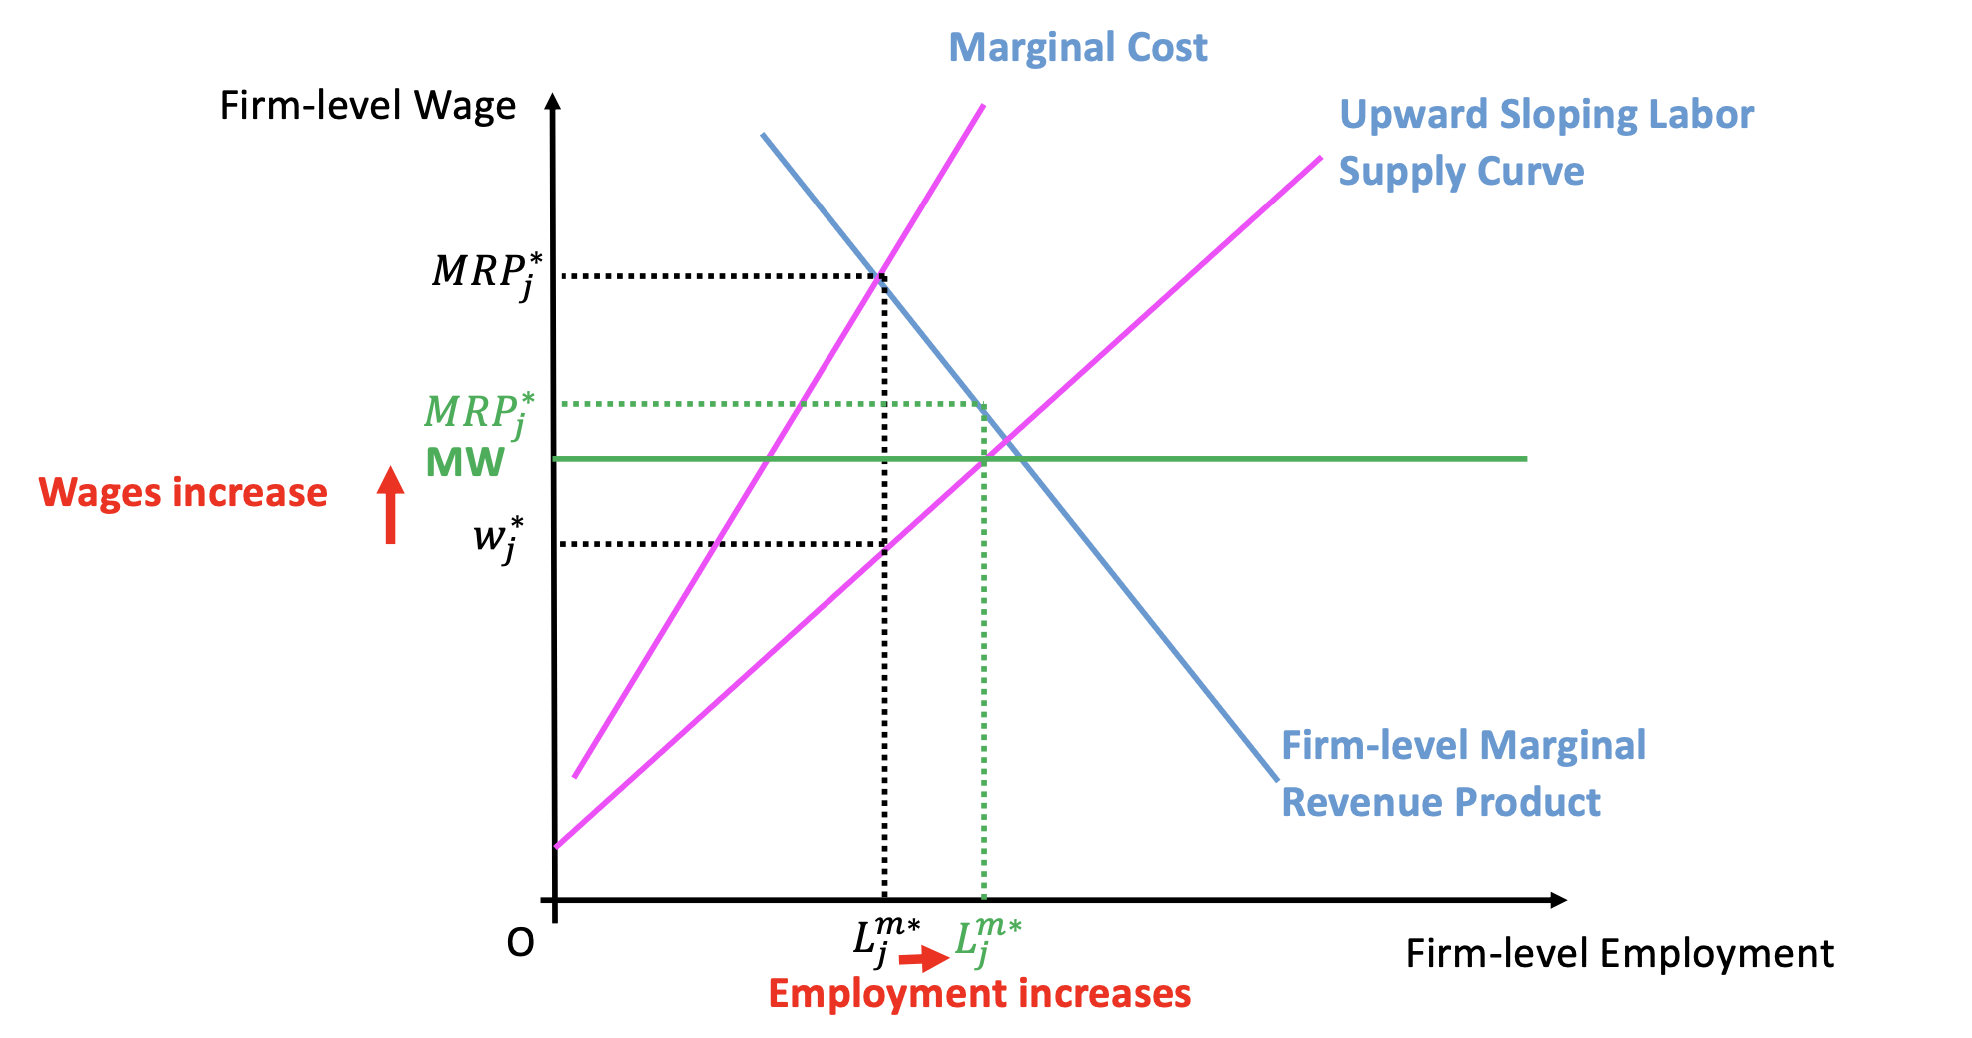
\includegraphics[width=5in]{images/ch2/Monop_LM_2.png}
            \caption{Minimum Wages in Monopsonistic Model}
        \end{figure}
        The overall effect is featured as a process called \emphb{reallocation}: \empha{employees of the least efficient firms are transferred to the more efficient one}. This improves efficiency. Meanwhile, though new firms pay more, workers might be worse off in other aspects, so the overall effect on welfare is still ambiguous.
        
    \subsection{Empirical Research on Reallocation}
        Historically, the role of reallocation has been featured prominently in the minimum wage debate since the later 19th century. (e.g. advocates to use minimum wage to stop the proliferation of "sweatshops" in the 1890s; Winston Churchill's argument for the Trade Boards Act 1909)
        
        \subsubsection{Dustmann, Lindner, Schönberg, Umkehrer, and vom Berge (2022)}
            Dustmann, Lindner, Schönberg, Umkehrer, and vom Berge (2022) provide direct evidence on the impact of the minimum wage on reallocation:
            \begin{itemize}
                \item Reform studied: Introduction of the minimum wage in Germany in 2015
                \item Data: Administrative employer-employee database covering the life history of all German private sector workers
                \item Empirical analysis: How wages, employment, and quality of the firm evolved following minimum wage hikes?
                \item Control groups:
                    \begin{itemize}
                        \item Projection based on the observed trend before the introduction of the minimum wage
                        \item Wage evolution at the higher end of the wage distribution
                    \end{itemize}
            \end{itemize}
            
        \subsubsection{Results}
            Positive wage increases for employees around the minimum wage:
            \begin{figure}[H]
                \centering
                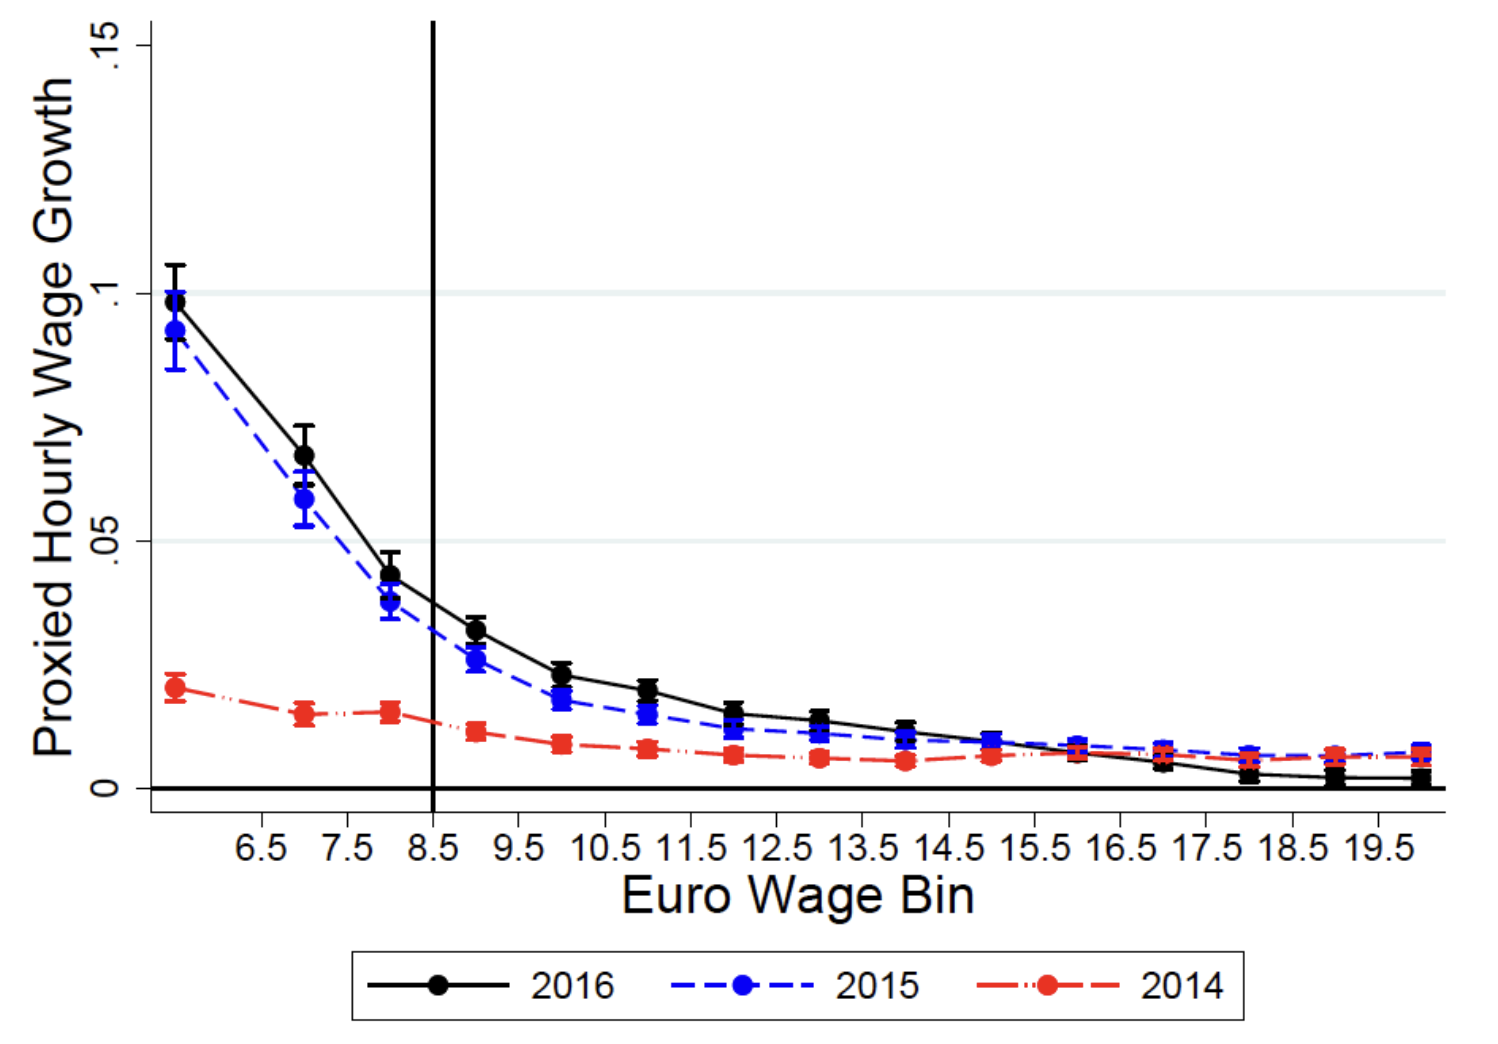
\includegraphics[width=4in]{images/ch2/reallocation_1.png}
                \caption{Wage Growth as a Function of Wages 2 Years Before}
            \end{figure}
            Increase in employment:
            \begin{figure}[H]
                \centering
                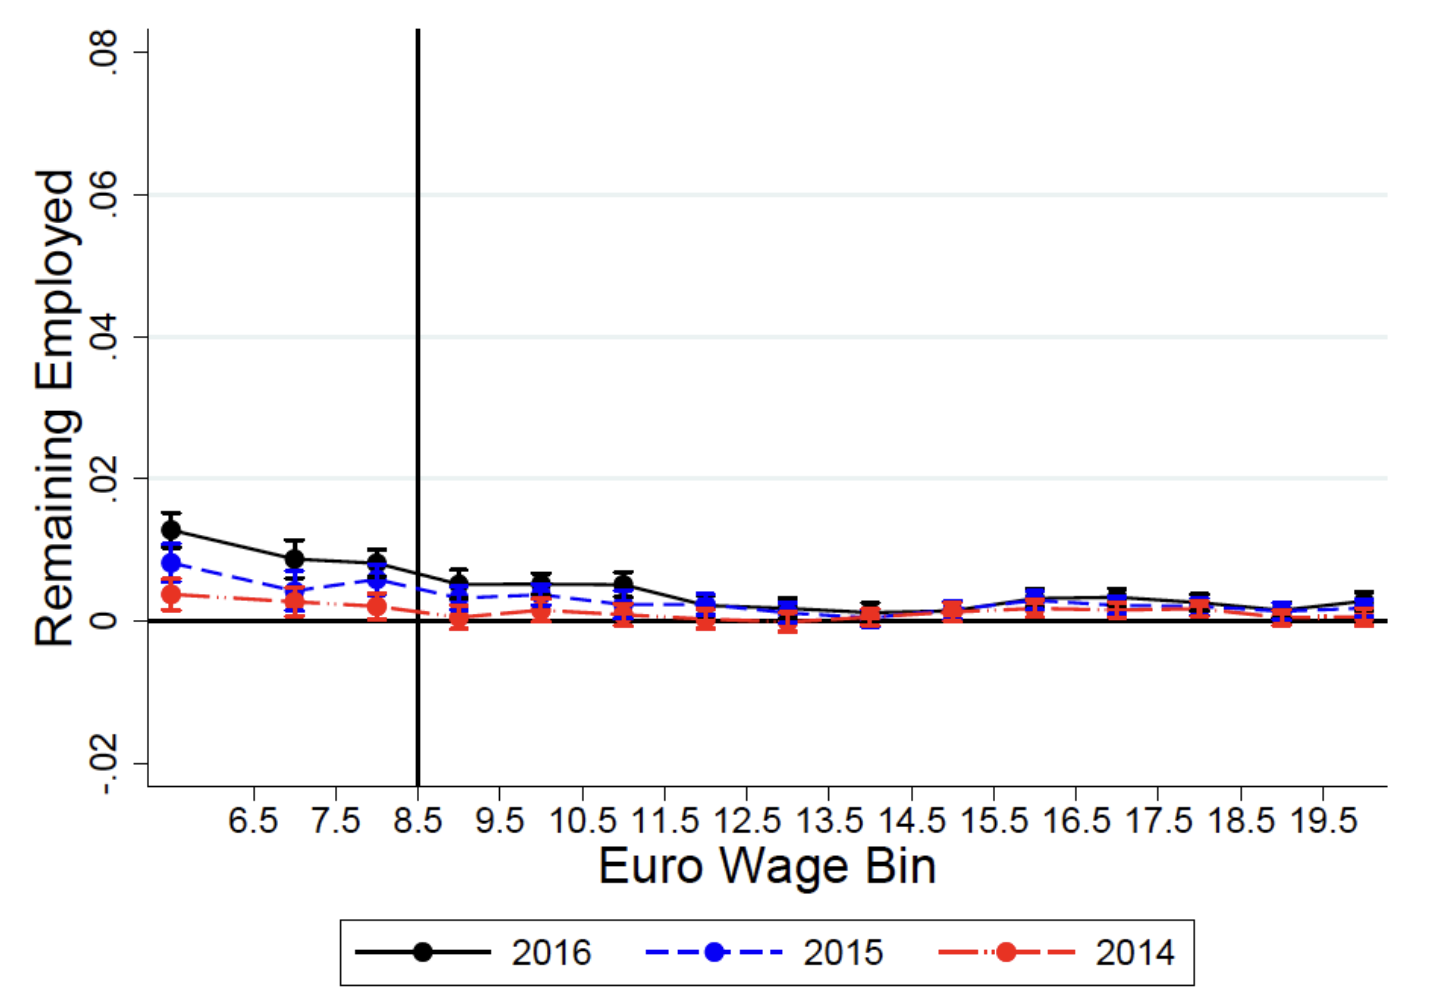
\includegraphics[width=4in]{images/ch2/reallocation_2.png}
                \caption{Employment Growth as a Function of Employment 2 Years Before}
            \end{figure}
            Higher wage premium:
            \begin{figure}[H]
                \centering
                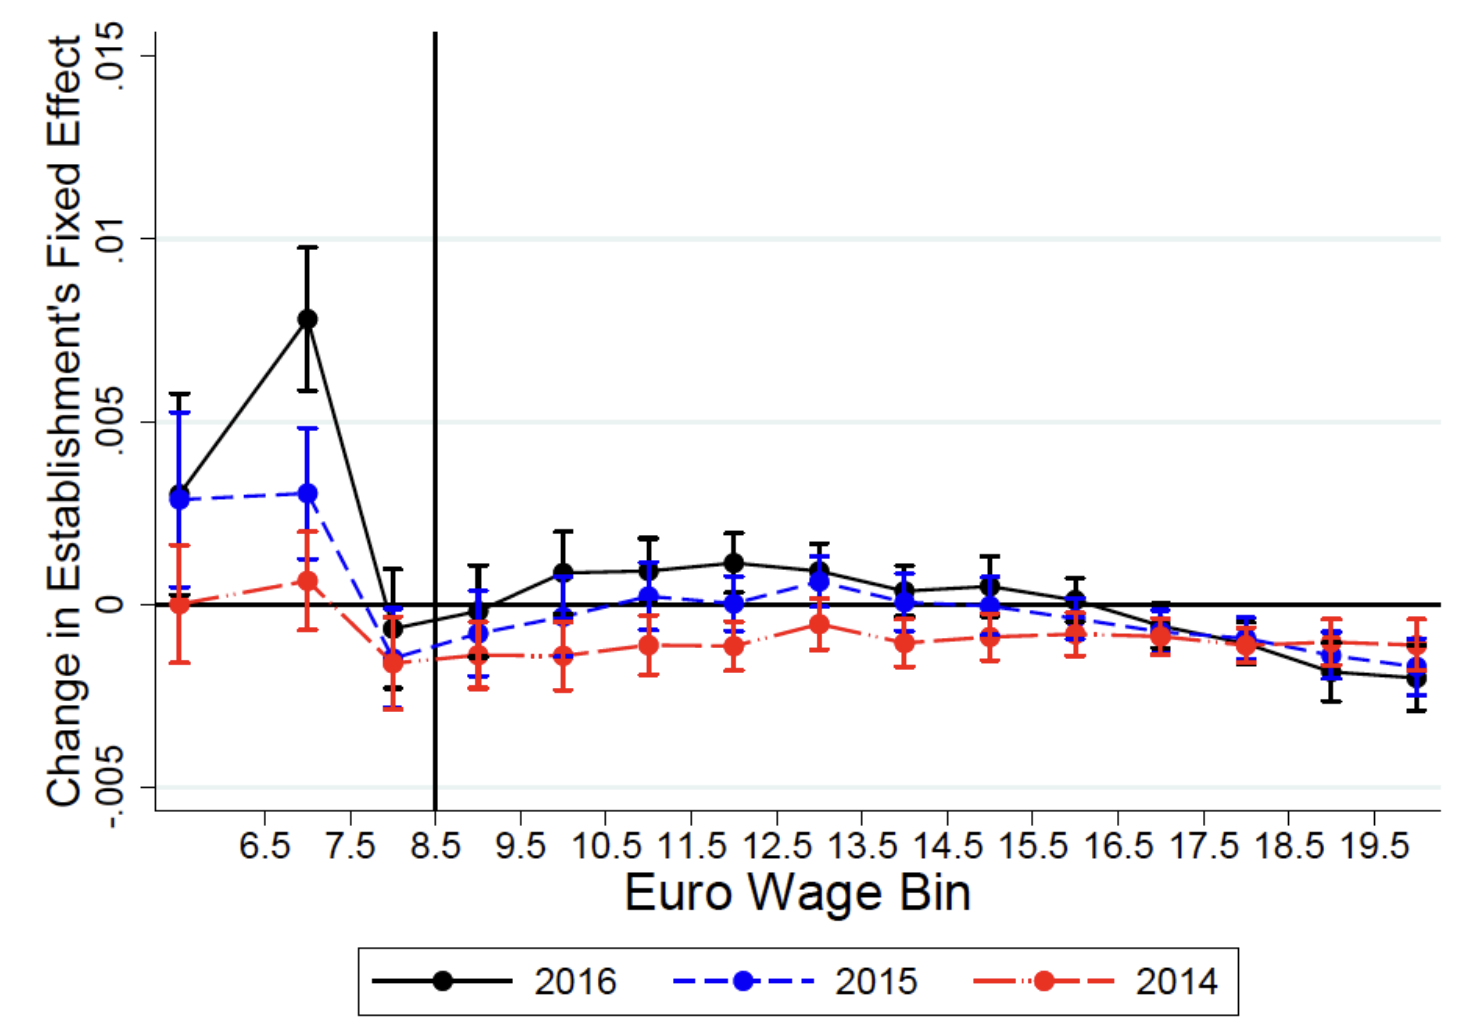
\includegraphics[width=4in]{images/ch2/reallocation_3.png}
                \caption{Firm Wage Premium as a Function of Wages 2 Years Before}
            \end{figure}
            Higher productivity:
            \begin{figure}[H]
                \centering
                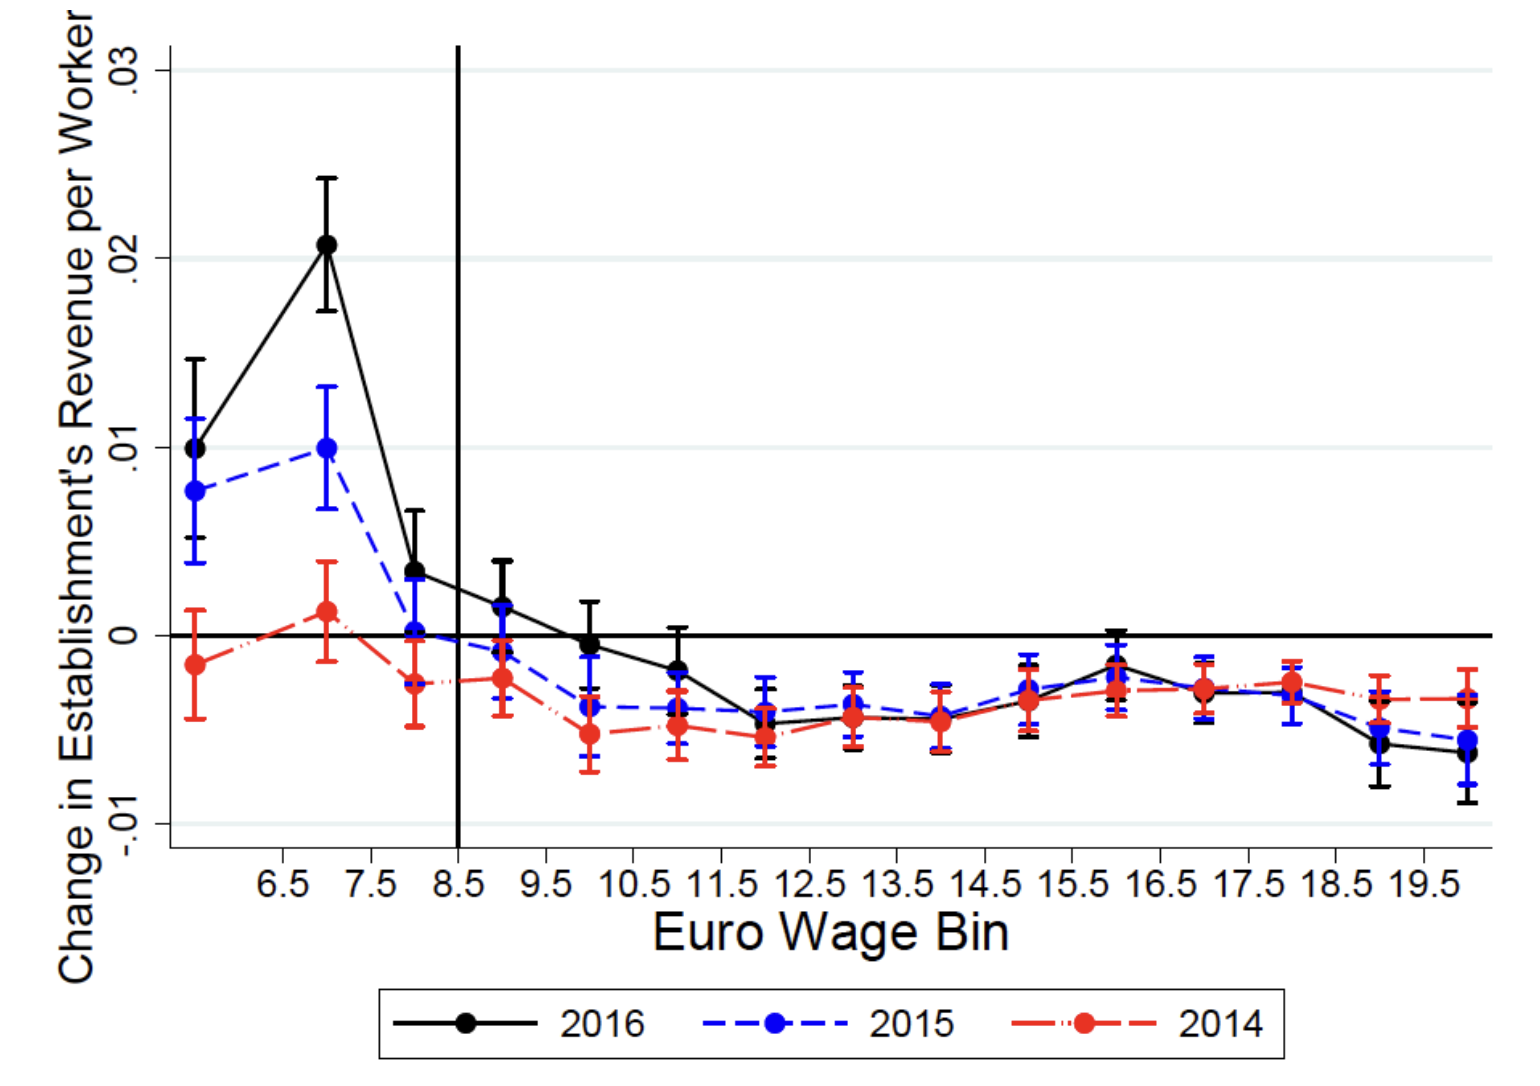
\includegraphics[width=4in]{images/ch2/reallocation_4.png}
                \caption{Firm’s Productivity Growth as a Function of Wages 2 Years Before}
            \end{figure}
            Reallocation from small firms to larger firms:
            \begin{figure}[H]
                \centering
                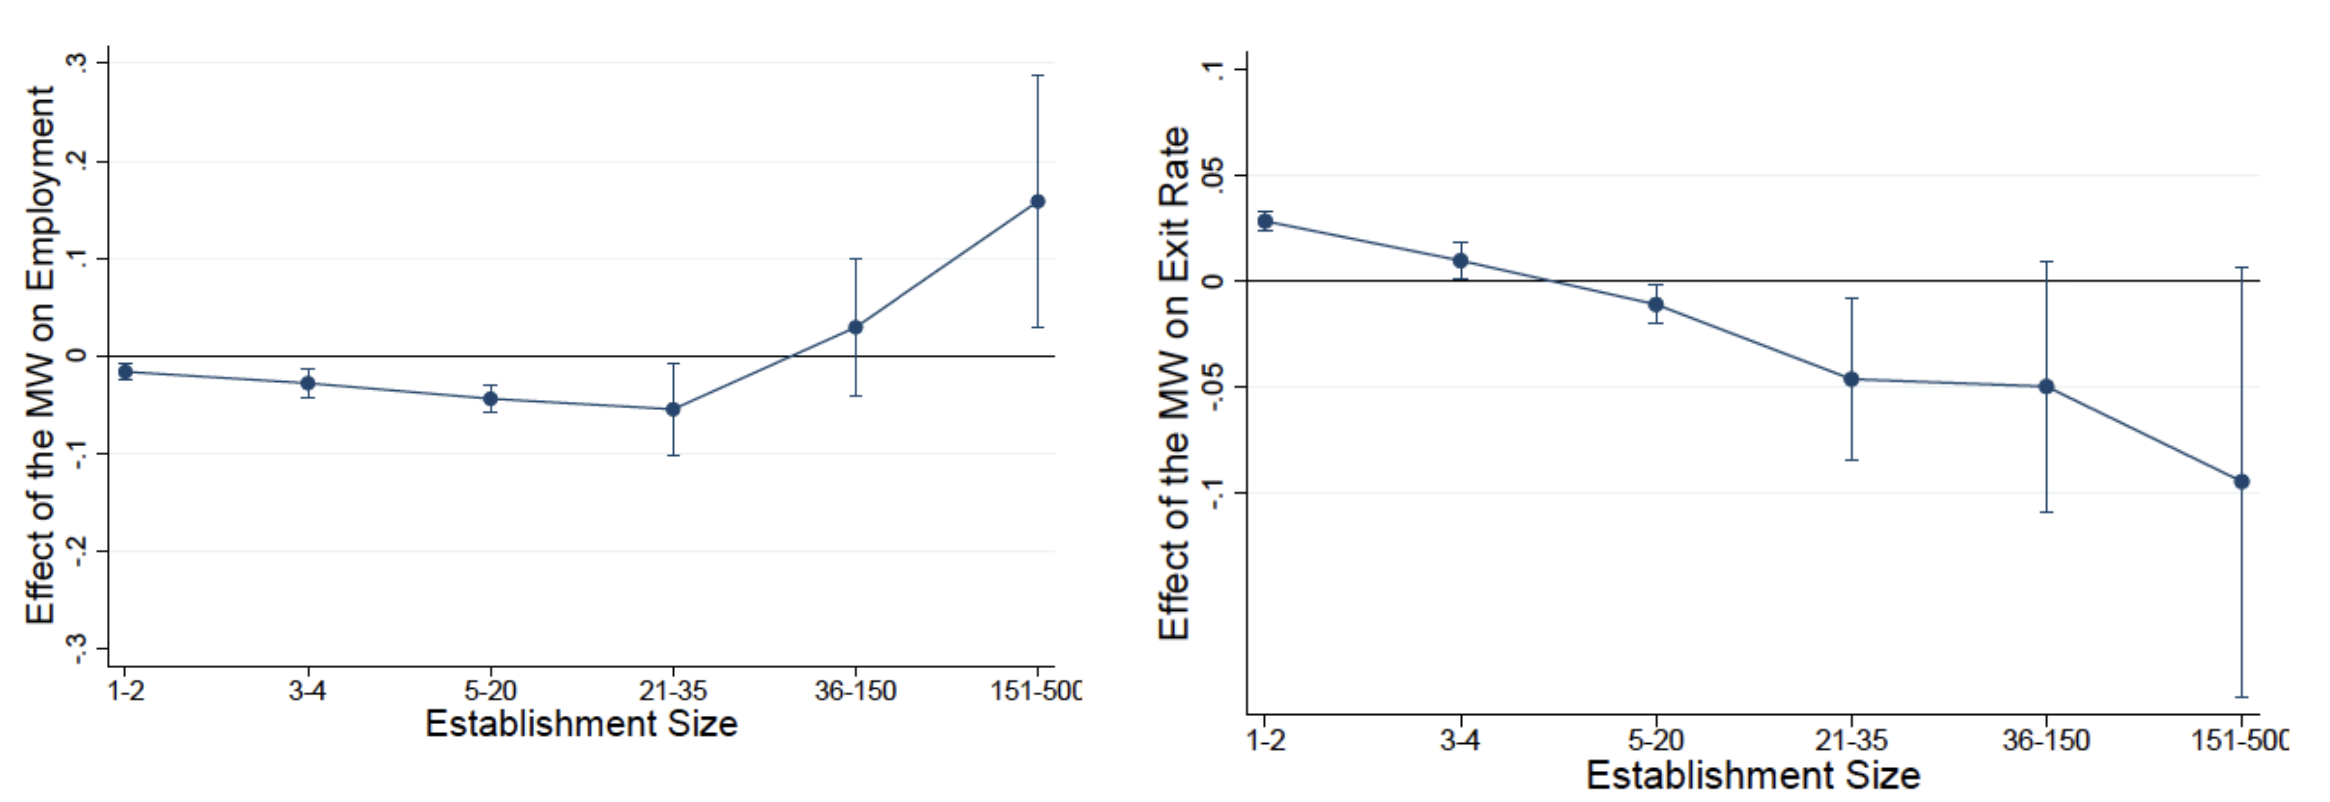
\includegraphics[width=5.5in]{images/ch2/reallocation_5.png}
                \caption{The Effect of the Minimum Wage by Firm Size}
            \end{figure}
            Key findings:
            \begin{itemize}
                \item Positive and significant effect on wages
                \item No dis-employment effect
                \item \emph{Reallocation} of workers to:
                \begin{itemize}
                    \item Firms paying higher wage premium
                    \item Firms with lower turnover
                    \item Firms with larger sizes higher productivity
                \end{itemize}
            \end{itemize}
            This indicates that minimum wages reallocate workers to more productive firms, contributing productivity improvement. The welfare implication is more ambiguous since there's evidence that workers' commuting distance increased.
\fi

%Topic 2: Health
\iftrue
   \chapter[Health as Human Capital]{Health as Human Capital\raisebox{.3\baselineskip}{\normalsize\footnotemark}}
\footnotetext{Written by Kuangjie Ni, Edited by Xiaotian Tian}

\fancyhead[L]{ECON0024}
\fancyhead[C]{Ch.3 Health as Human Capital}
\fancyhead[R]{Kuangjie Ni}
\fancyfoot[L]{\hyperlink{tableofcontents}{Back to Table of Contents}}
\fancyfoot[R]{Kuangjie Ni}

\section{Intro: Why are some of us less healthy than others?}

    \begin{itemize}
        \item Bad genes
        \item Bad lifestyles
        \item Poor healthcare 
        \item Poor early environment 
        (e.g. poor parenting, mum drinking during pregnancy)
   \end{itemize}    

\section{Health Spending}

    \subsection{Facts about Health Spending: Global}

        \subsubsection{Health spending per capita}

            \begin{figure}[H]
                \centering
                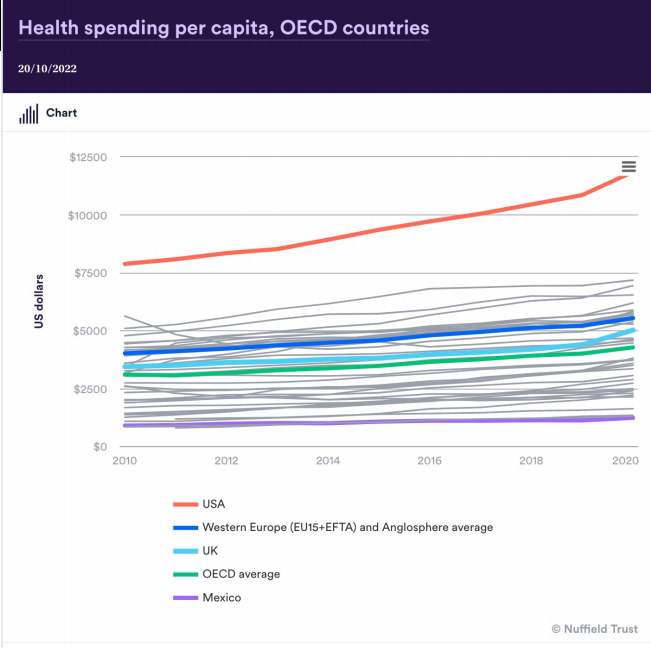
\includegraphics[width=3in]{images/ch3/1 Health spending OECD.png}
                \caption{Health Spending per Capita, OECD countries}
            \end{figure}
            \begin{itemize}
                \item Health spending per capita is increasing over time. People are living longer than they used to be. The longer you live, the sicker you get and the more money you spend on healthcare. 
                \item US has a higher health spending and a particular healthcare structure.
            \end{itemize}
        
        \subsubsection{A Large Fraction Is Government/Compulsory Spending}
            \begin{figure}[H]
                \centering
                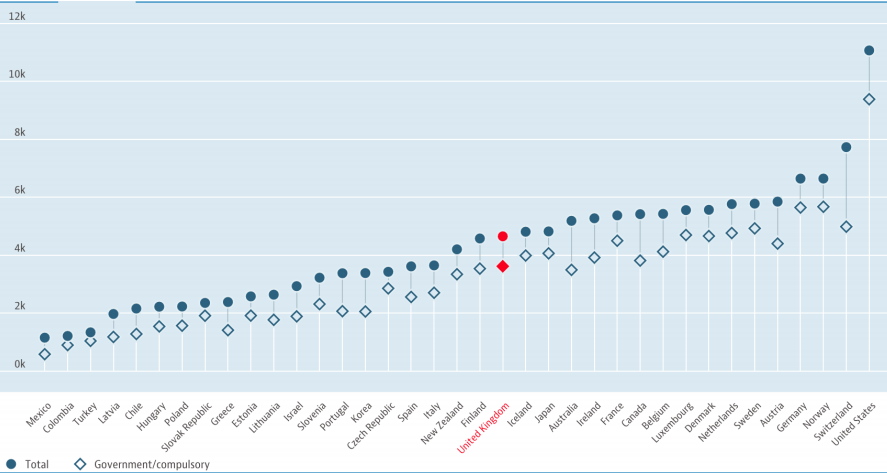
\includegraphics[width=5in]{images/ch3/2 Government.png}
                \caption{Health spending: Total including government/compulsory spending in US dollars/capita, 2019}
            \end{figure}      
            \begin{itemize}
                \item Blue dots are the total health spending, and diamonds are the government/compulsory spending. 
                \item US government spends a lot of money on healthcare.
            \end{itemize}
        
        \subsubsection{Total Spending as \% of GDP}
            \begin{figure}[H]
                \centering
                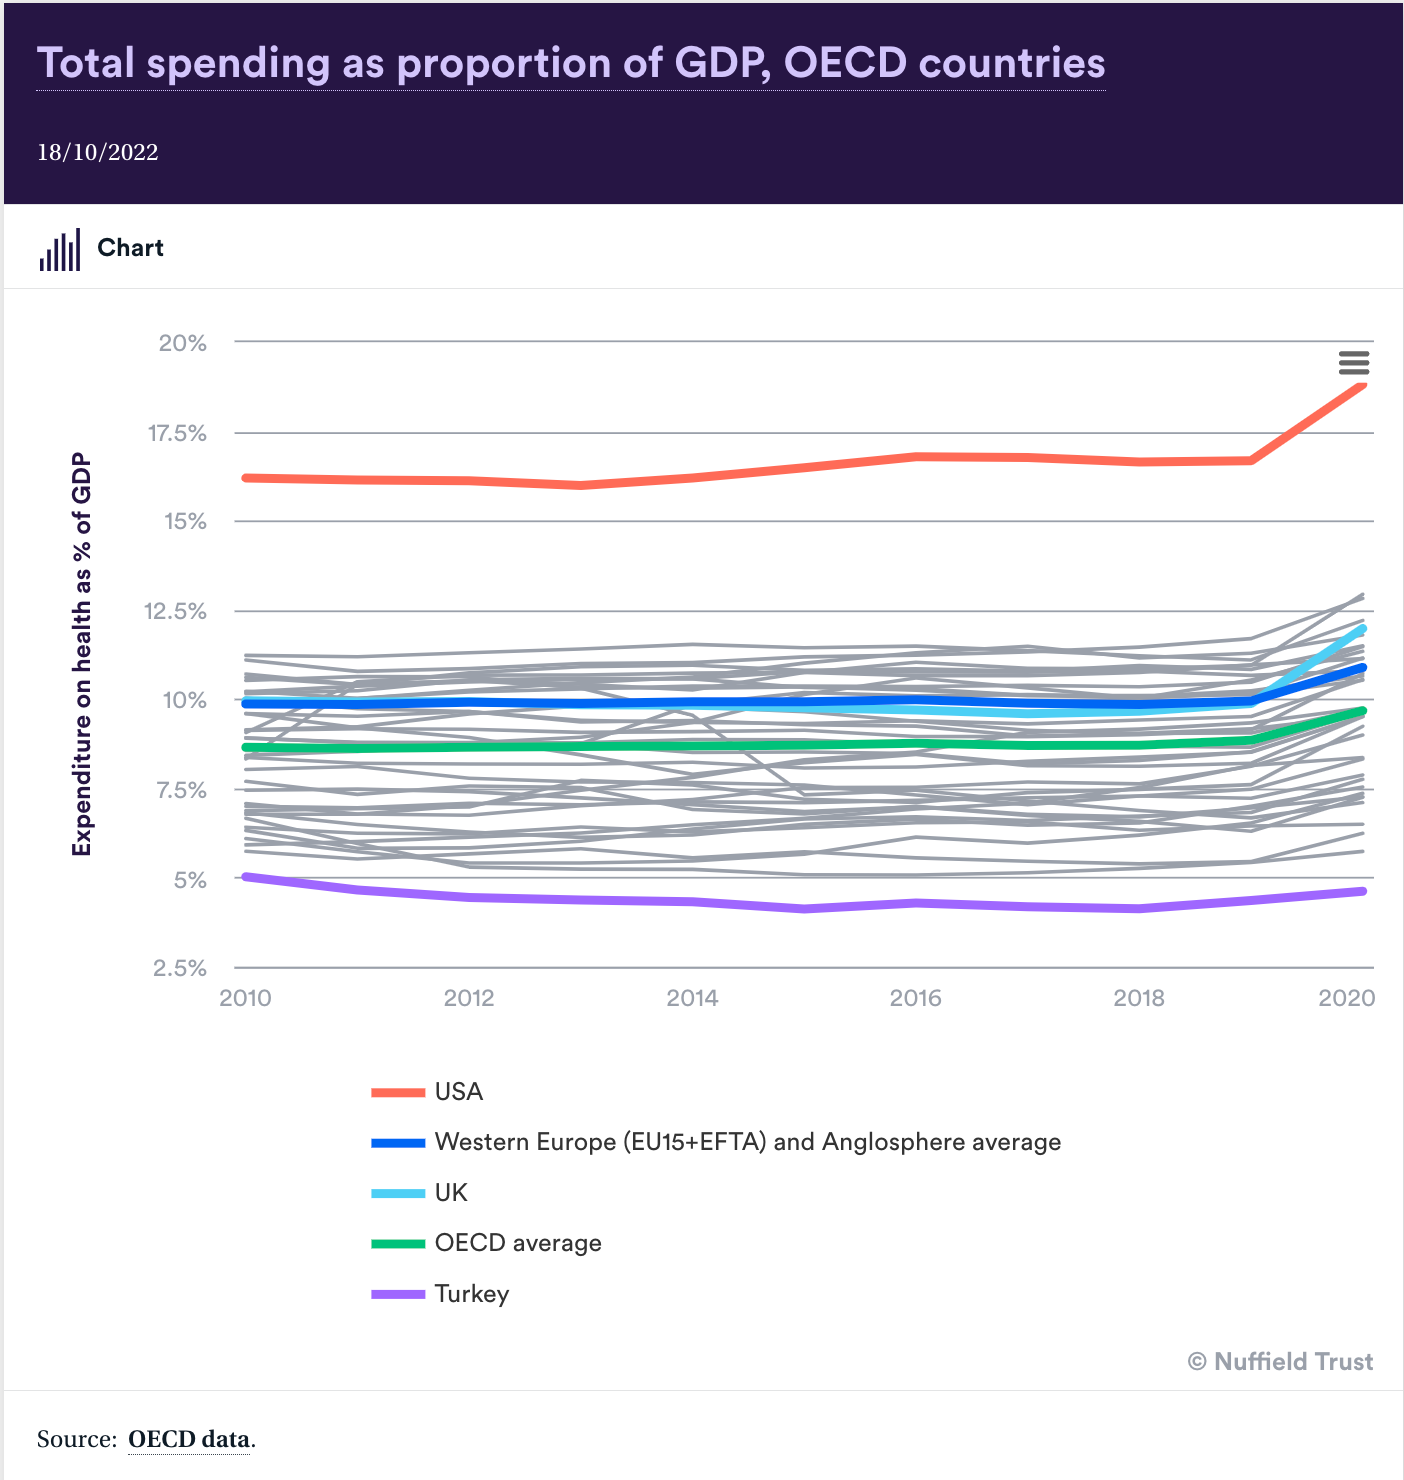
\includegraphics[width=4in]{images/ch3/3 GDP.png}
                \caption{Total spending as a proportion of GDP, OECD countries}
            \end{figure}            
            \begin{itemize}
                \item US has the highest health spending as a proportion of GDP.
                \item The total health spending as a proportion of GDP increased during the pandemic.
            \end{itemize}
        
    \subsection{Facts about Health Spending: the UK}
    
        \subsubsection{Health as \% of UK Total Spending}  
            \begin{figure}[H]
                \centering
                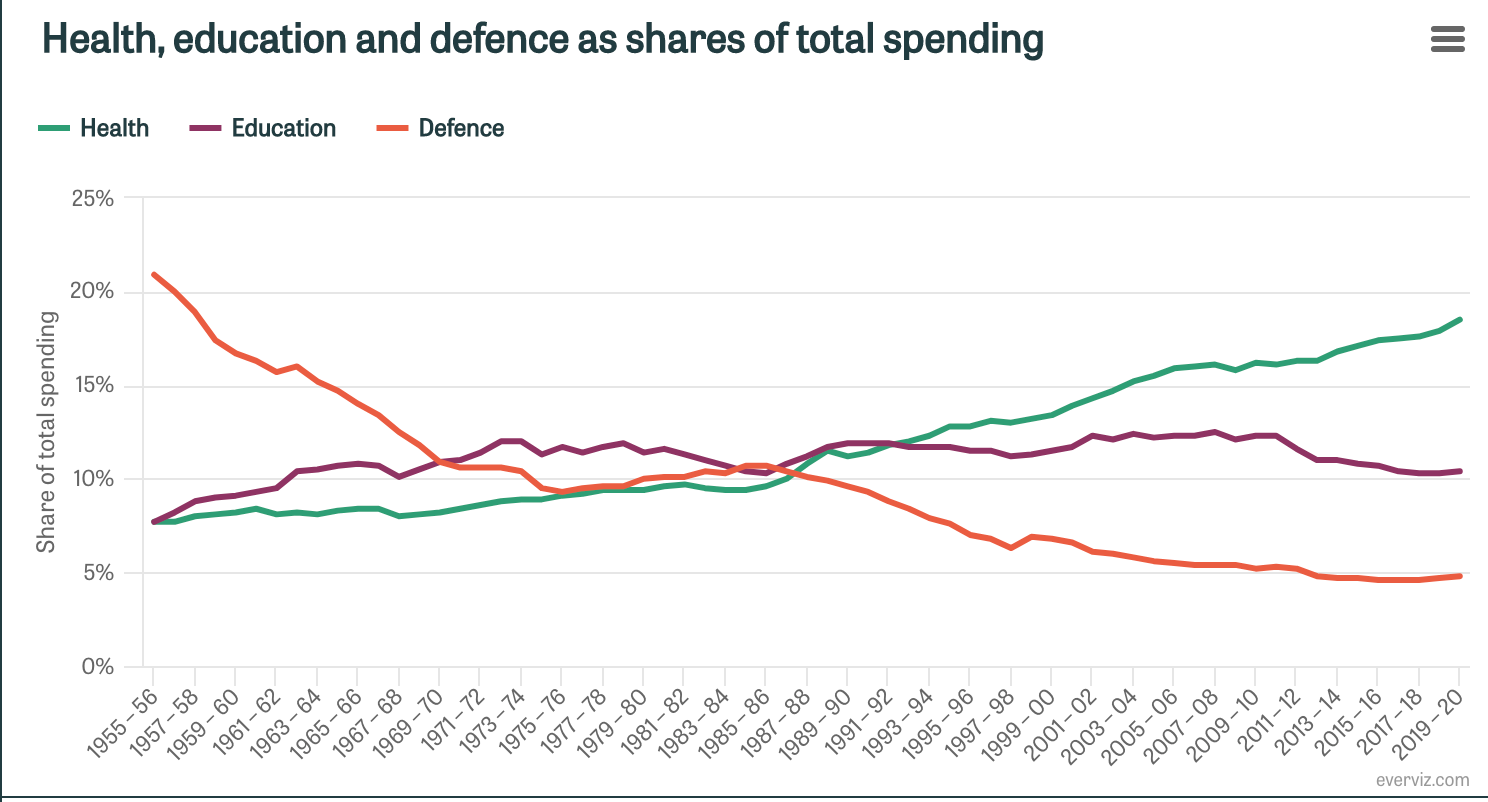
\includegraphics[width=4in]{images/ch3/4.png}
                \caption{Health, education and defence as shares of total spending}
            \end{figure} 
        \begin{itemize}           
            \item Health spending takes a bigger share of total UK spending over the last 70 years.
            \item The share of education spending is approximately flat, and the share of defence spending declines significantly.
        \end{itemize}
        
        \subsubsection{Components of UK Government Spending}  
            \begin{figure}[H]
                \centering
                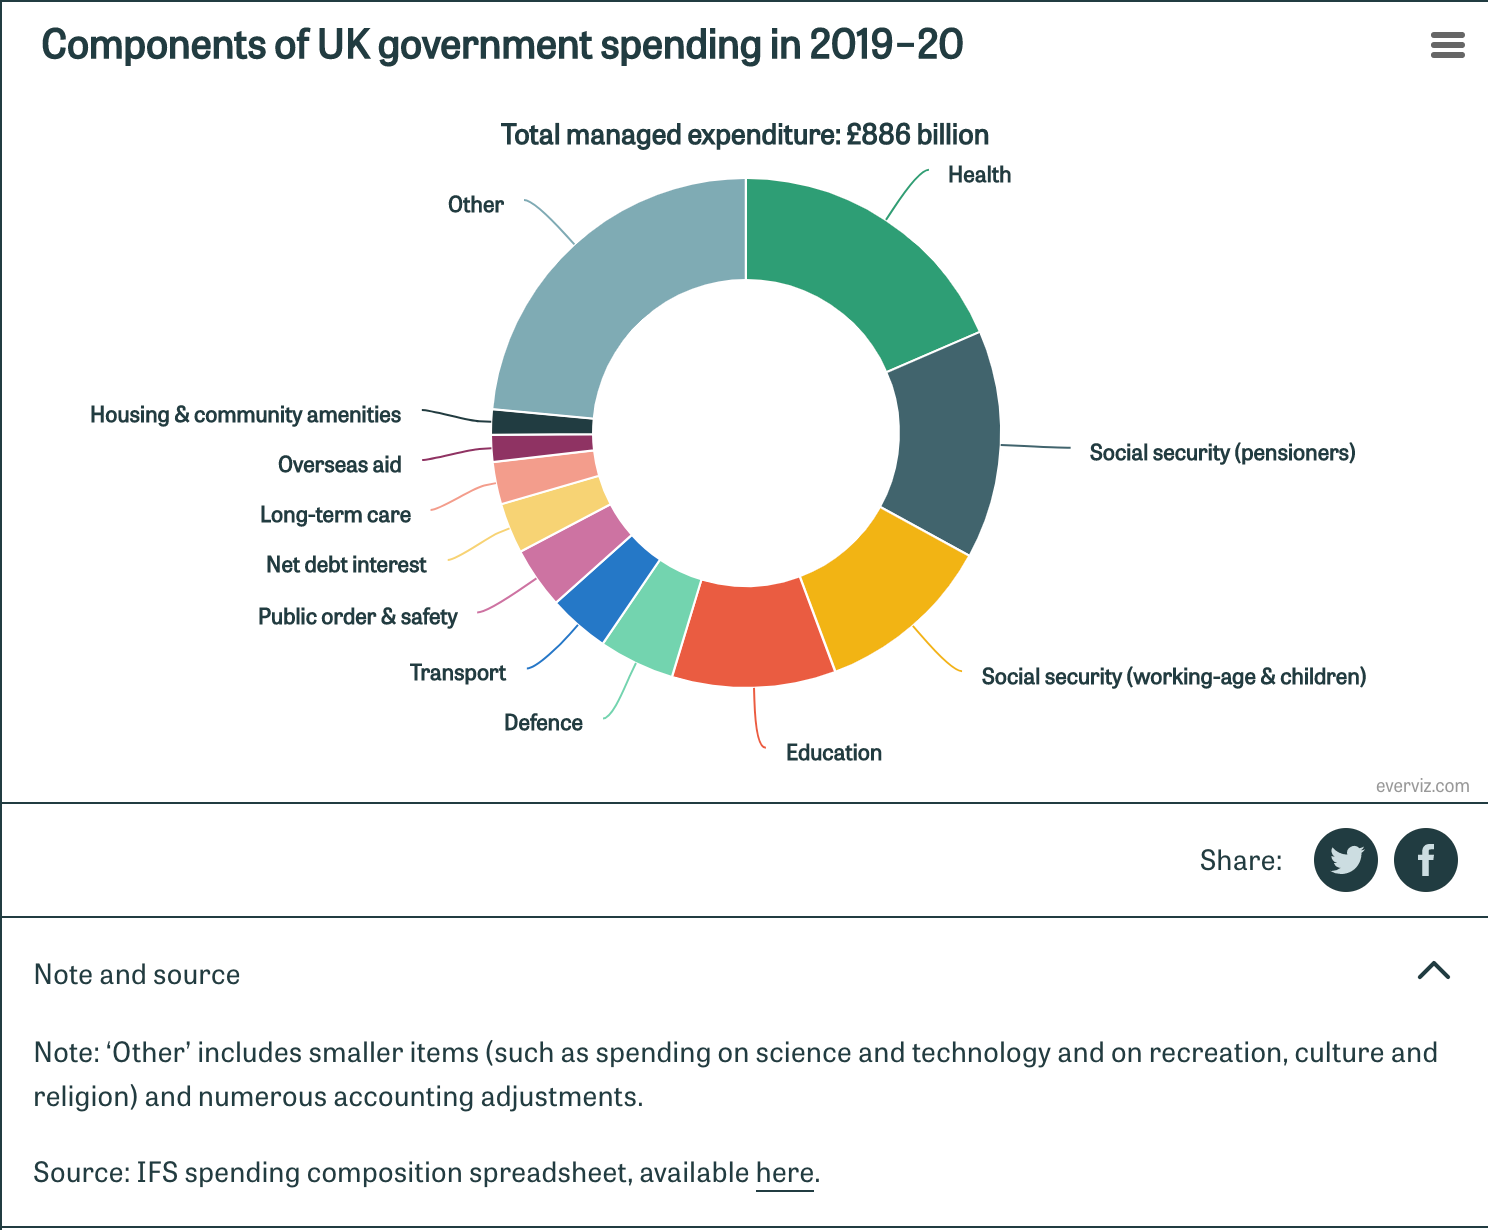
\includegraphics[width=4in]{images/ch3/5.png}
                \caption{Components of UK GOV spending in 2019-20}
            \end{figure} 
            Total managed UK government expenditure is 886 billion pounds, and health spending is a very important component.

        \subsubsection{UK Public Spending on Health}         
            \begin{figure}[H]
                \centering
                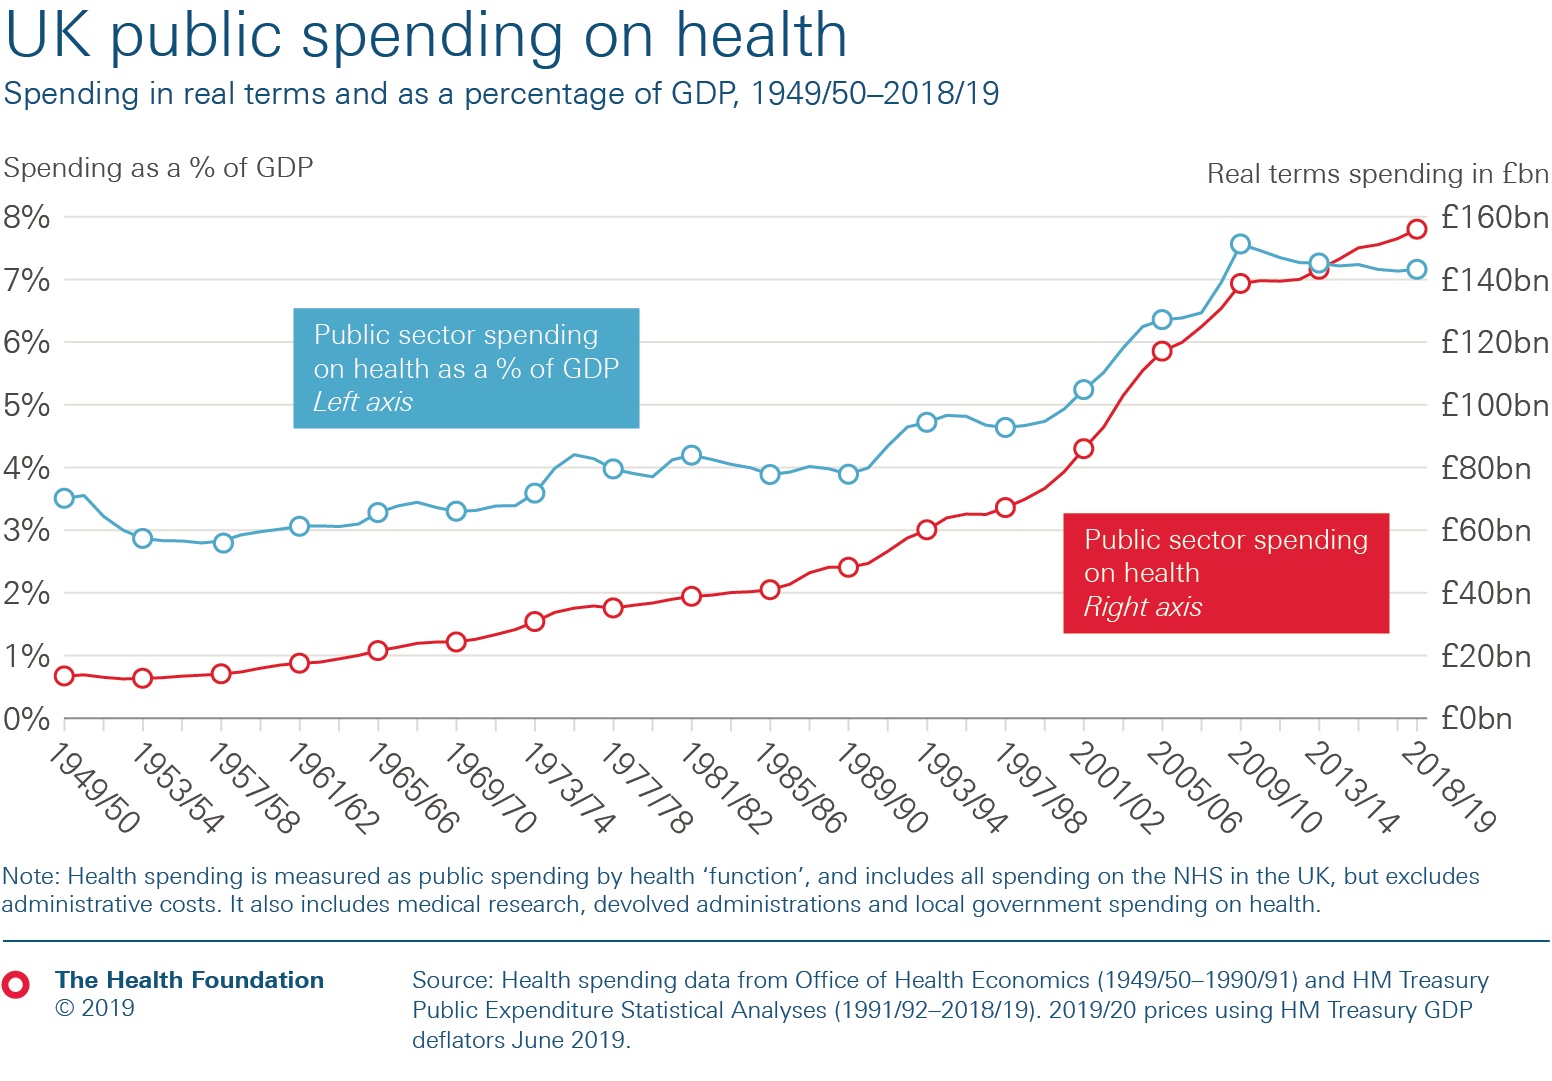
\includegraphics[width=4in]{images/ch3/6.png}
                \caption{UK public spending on health, 1949/50 - 2018/19}
            \end{figure} 
            \begin{itemize}           
                \item The blue line shows the UK public sector spending on health as a percentage of GDP (left axis). The red line shows the UK public sector spending on health in real terms (right axis).
                \item The UK public sector spending on health has increased both as a percentage of GDP and in real terms since the end of World War II.
            \end{itemize}

        \subsubsection{Department of Health and Social Care spending} 
            \begin{figure}[H]
                \centering
                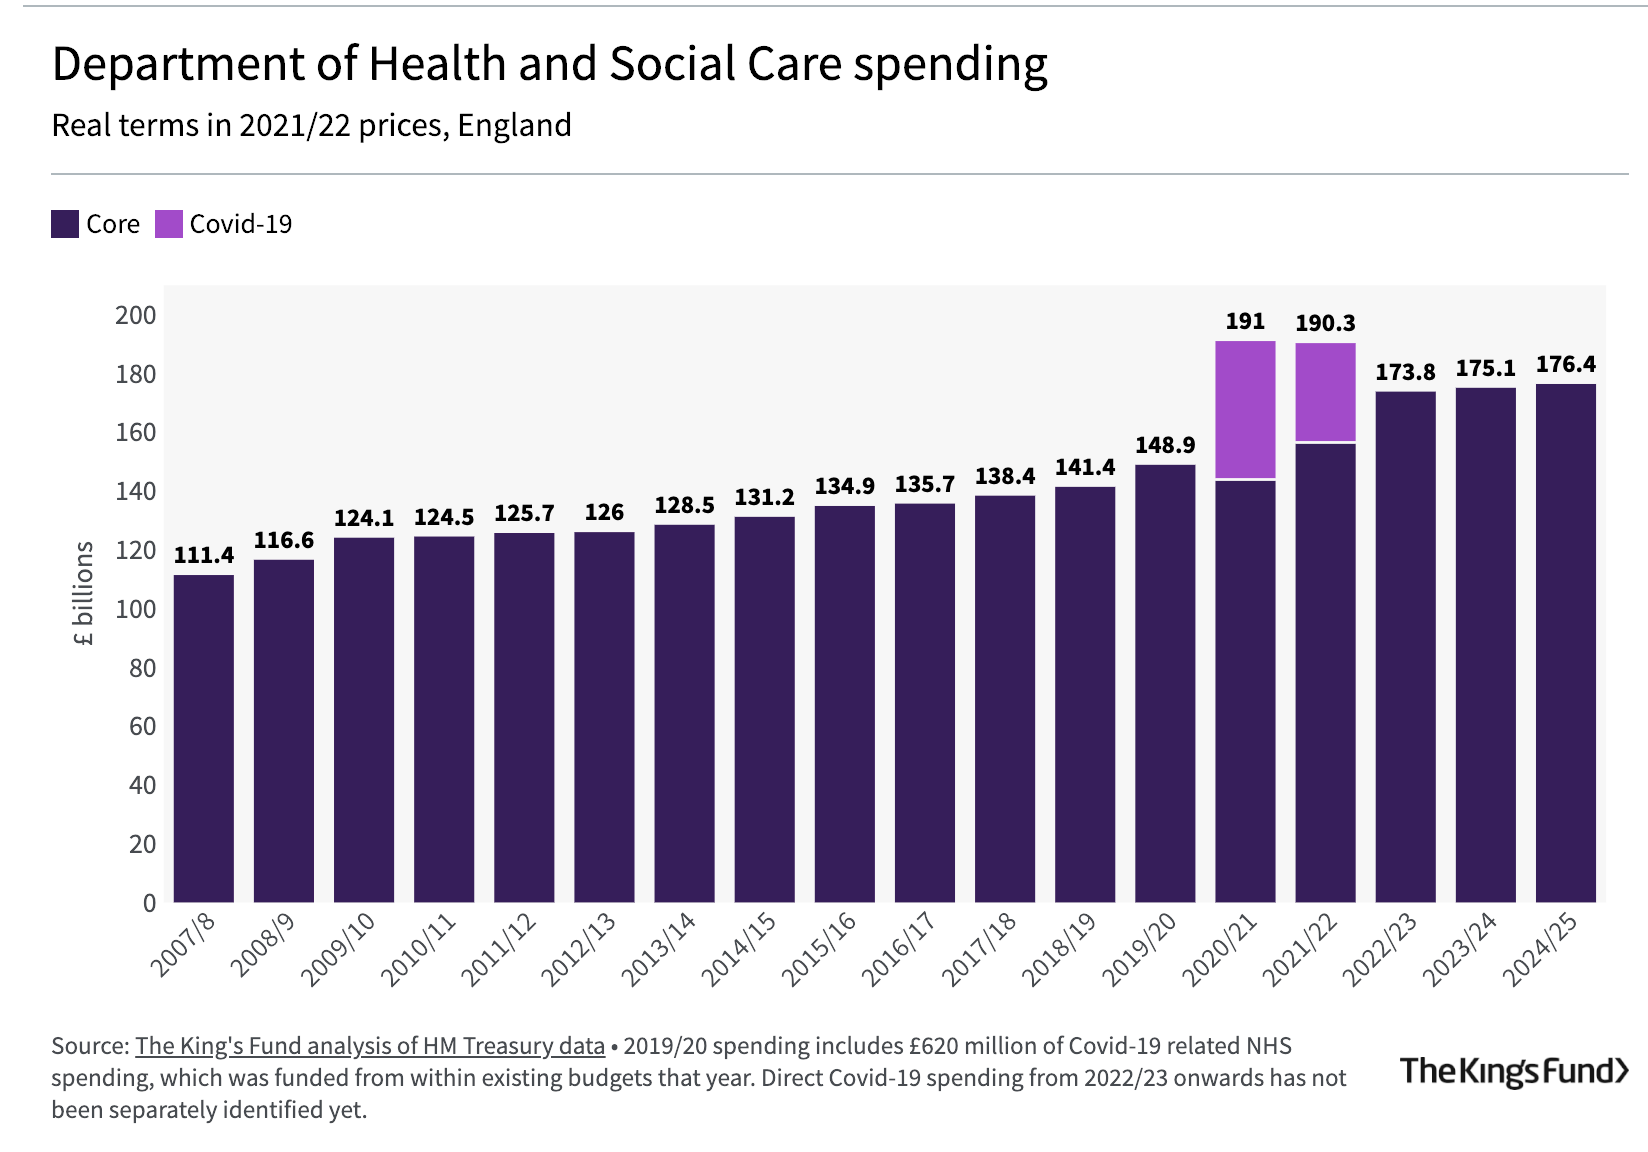
\includegraphics[width=4in]{images/ch3/7.png}
                \caption{Department of Health and Social Care spending, real terms in 2021/22 prices, England}
            \end{figure} 
                The Department of Health and Social Care spending increased a lot due to Covid-19, and the core spending keeps going up after 2021/22.

        \subsubsection{UK Health Spending Growth} 
            \begin{figure}[H]
                \centering
                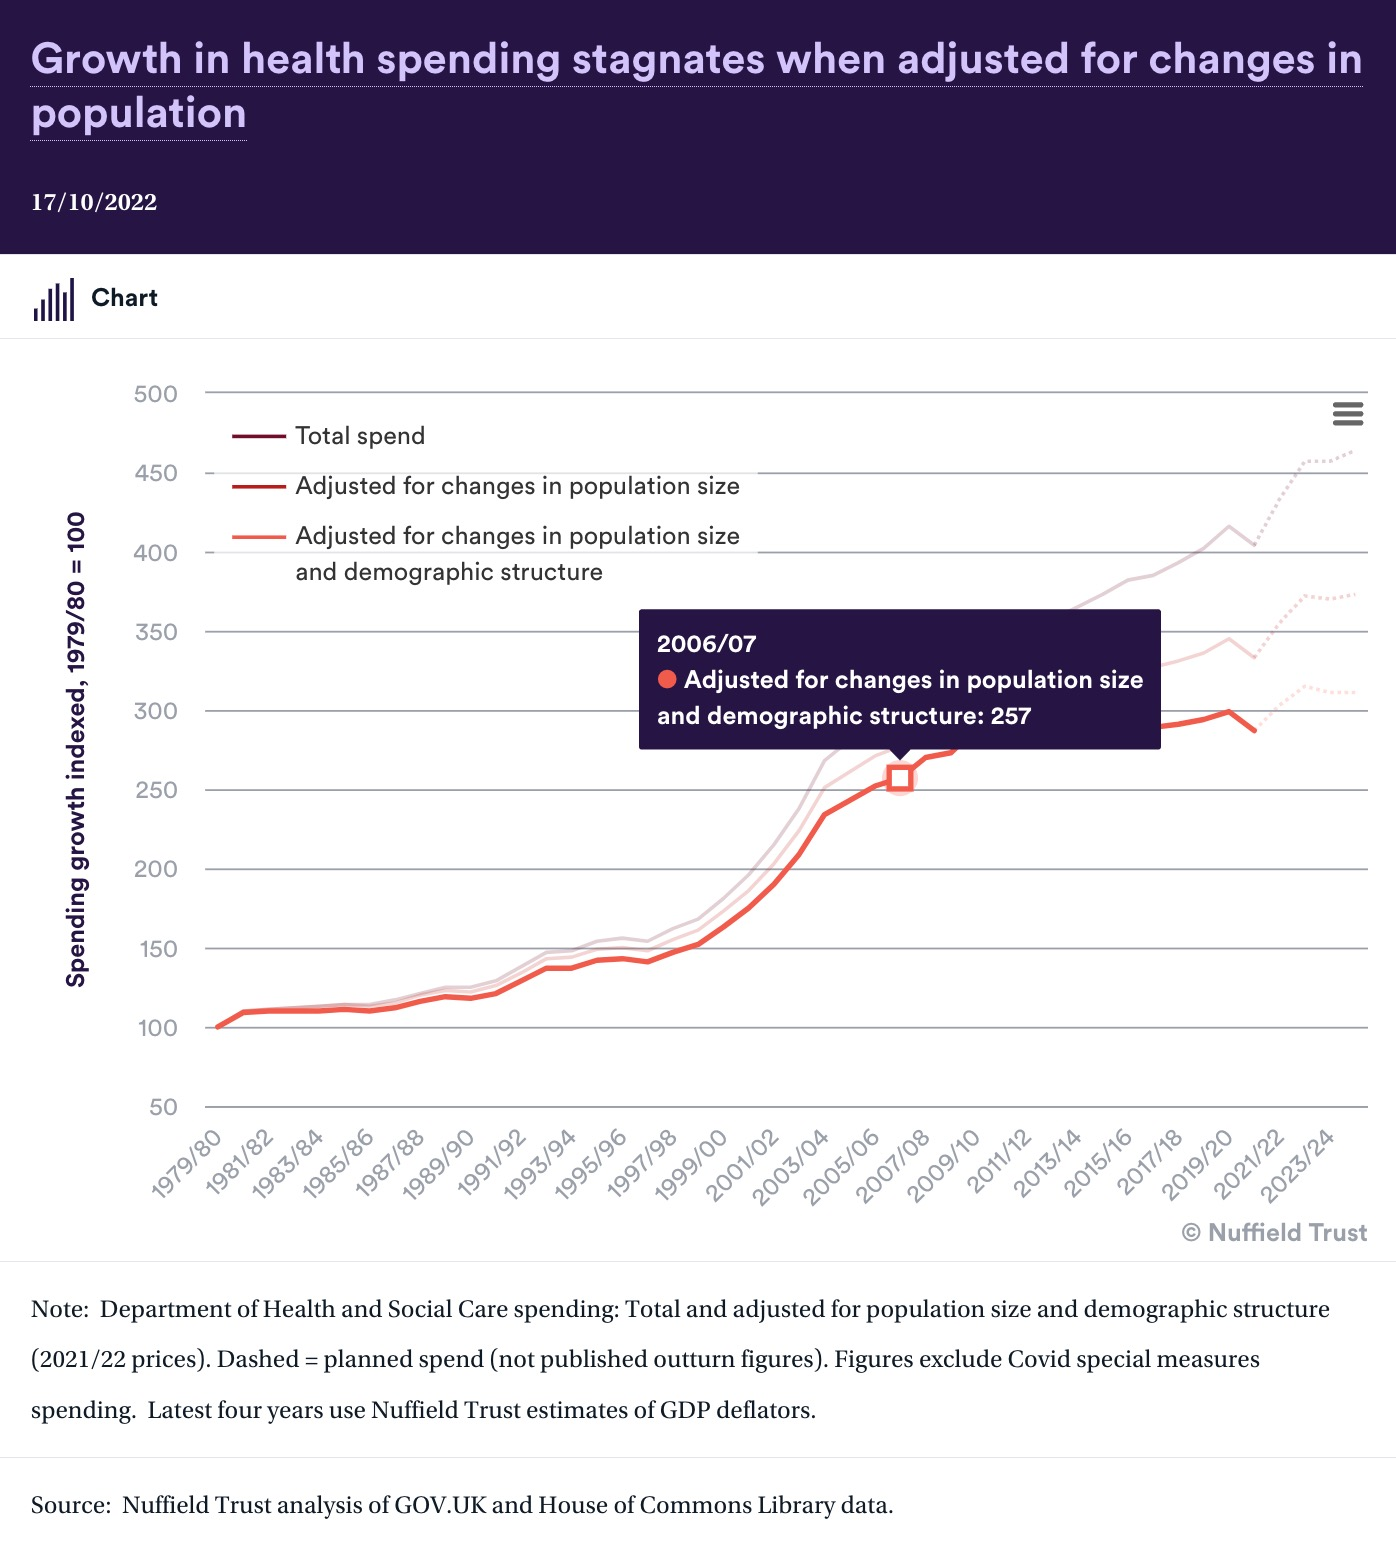
\includegraphics[width=4in]{images/ch3/8.png}
                \caption{Health spending growth indexed, 1979/80 = 100}
            \end{figure} 
            \begin{itemize}           
                \item The dark red line shows the total health spending. The red line shows the total health spending adjusted for changes in population size. The orange line shows the total health spending adjusted for changes in population size and demographic structure.
                \item Growth in health spending stagnates after adjusted for changes in population (population ageing).
            \end{itemize}       
            \begin{figure}[H]
                \centering
                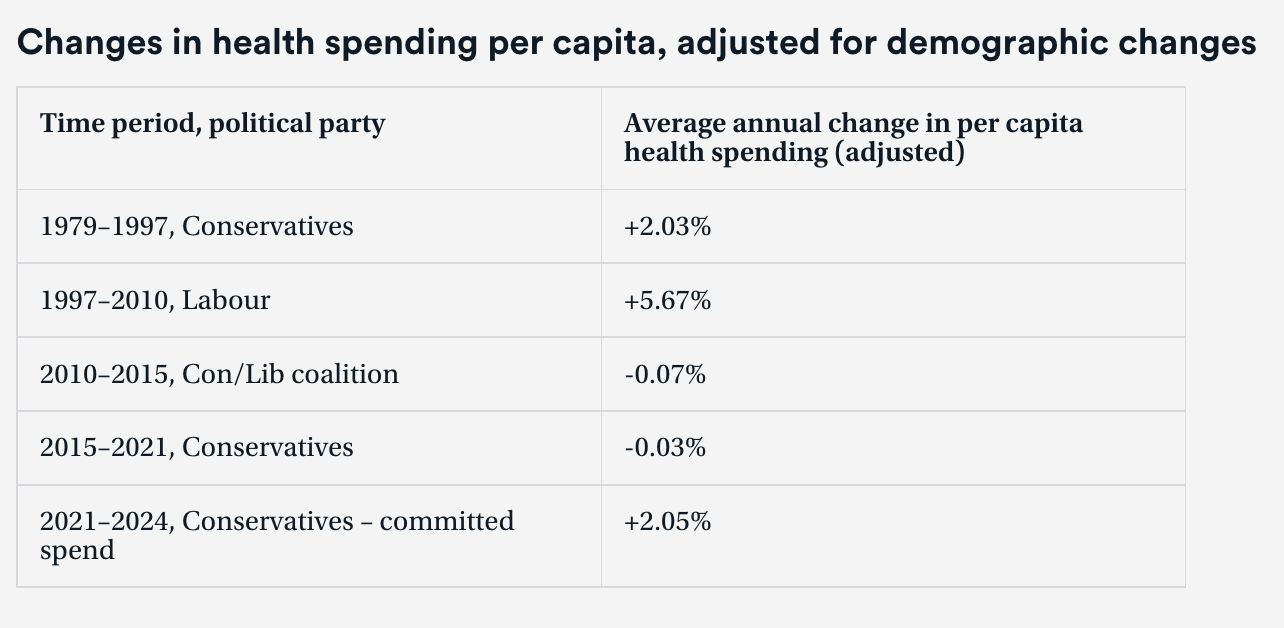
\includegraphics[width=4in]{images/ch3/9.png}
                \caption{Changes in health spending per capita, adjusted for demographic changes}
            \end{figure} 
            The Labour government has the highest increase in health spending per capita.

    \subsection{How Is the Health Budget Spent?}

        \subsubsection{}




        \subsubsection{How funding flows in the NHS?} 
            \begin{figure}[H]
                \centering
                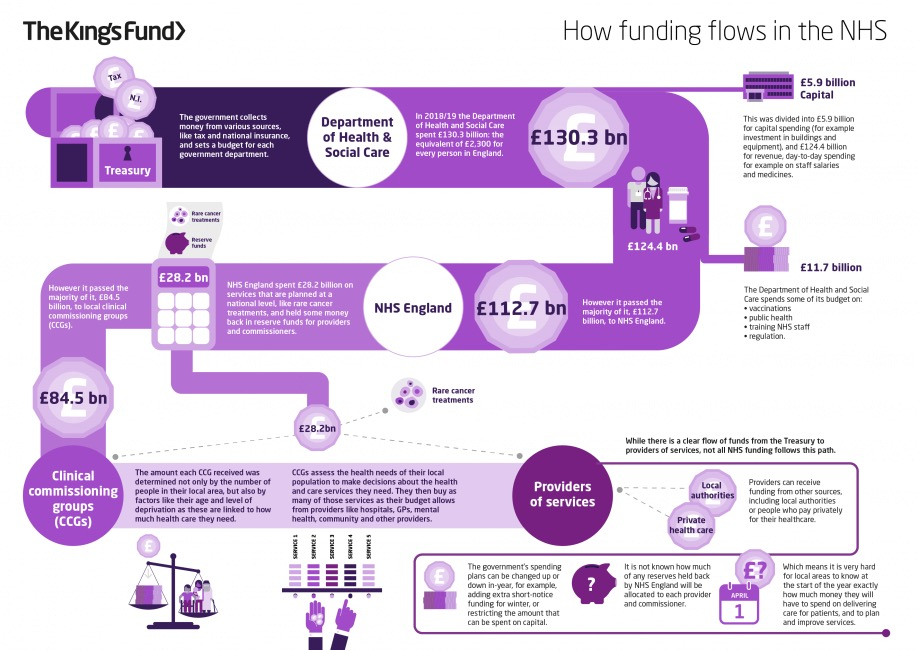
\includegraphics[width=5in]{images/ch3/11.png}
                \caption{How funding flows in the NHS?}
            \end{figure} 
            \begin{itemize}           
                \item In 2018/19, the Treasury gave the Department of Health and Social Care 130.3 billion pounds. This was divided into 5.9 billion for capital spending and 124.4 billion for day-to-day spending. 
                \item The 124.4 billion was further divided into 11.7 billion for preventive services (vaccinations, public health, training NHS staff, and regulation) and 112.7 billion for NHS England. 
                \item NHS England spent 28.2 billion on national-planned services, such as rare cancer treatments, and passed the remaining 84.5 billion to the clinical commissioning groups (CCGs). The amount each CCG received was determined by the number of people in the local area and by factors such as age (how sick they are).
            \end{itemize} 

        \subsubsection{Example: Bradford CCG}         
            \begin{figure}[H]
                \centering
                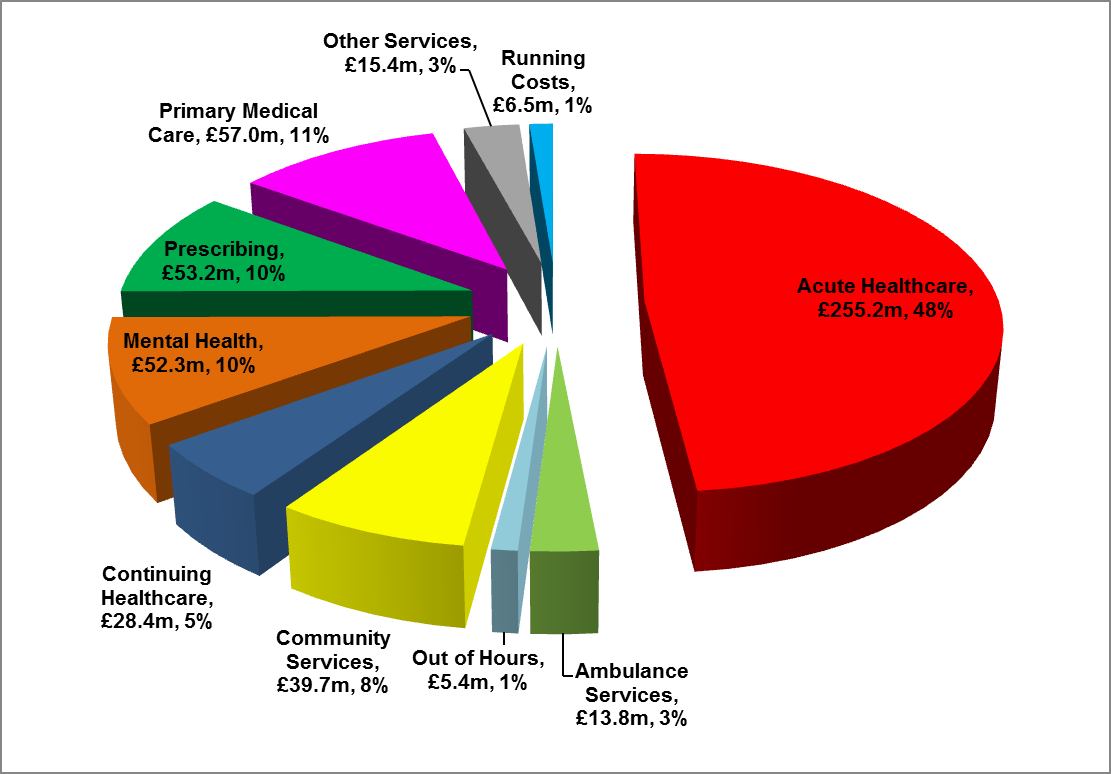
\includegraphics[width=4in]{images/ch3/12.png}
                \caption{Total CCG net expenditure, 2019/20(526.9 million pounds)}
            \end{figure} 
            Half of the money goes to acute healthcare. A small proportion of the money goes to preventive services, such as community services (health visitors and immunisation).
        
        \subsection{Preventive Care}
        
             \subsection{Other Factors that Matter to Health other than Healthcare} 
                \begin{figure}[H]
                    \centering
                    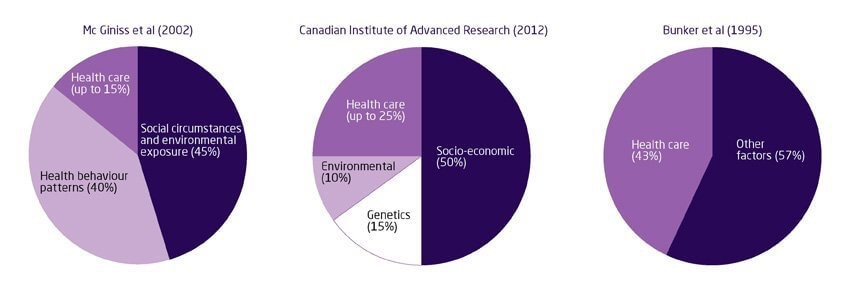
\includegraphics[width=5in]{images/ch3/14.png}
                    \caption{There is more to health than healthcare}
                \end{figure} 
                These three pie charts show the proportion of health that does not depend on the healthcare. Although the proportion varies between different studies, healthcare matters by less than a half in all studies.
    
            \subsubsection{Example: The role of lifestyles in the prevention of chronic conditions}         
            \begin{figure}[H]%option [H] means "strictly here"
                    \centering
                    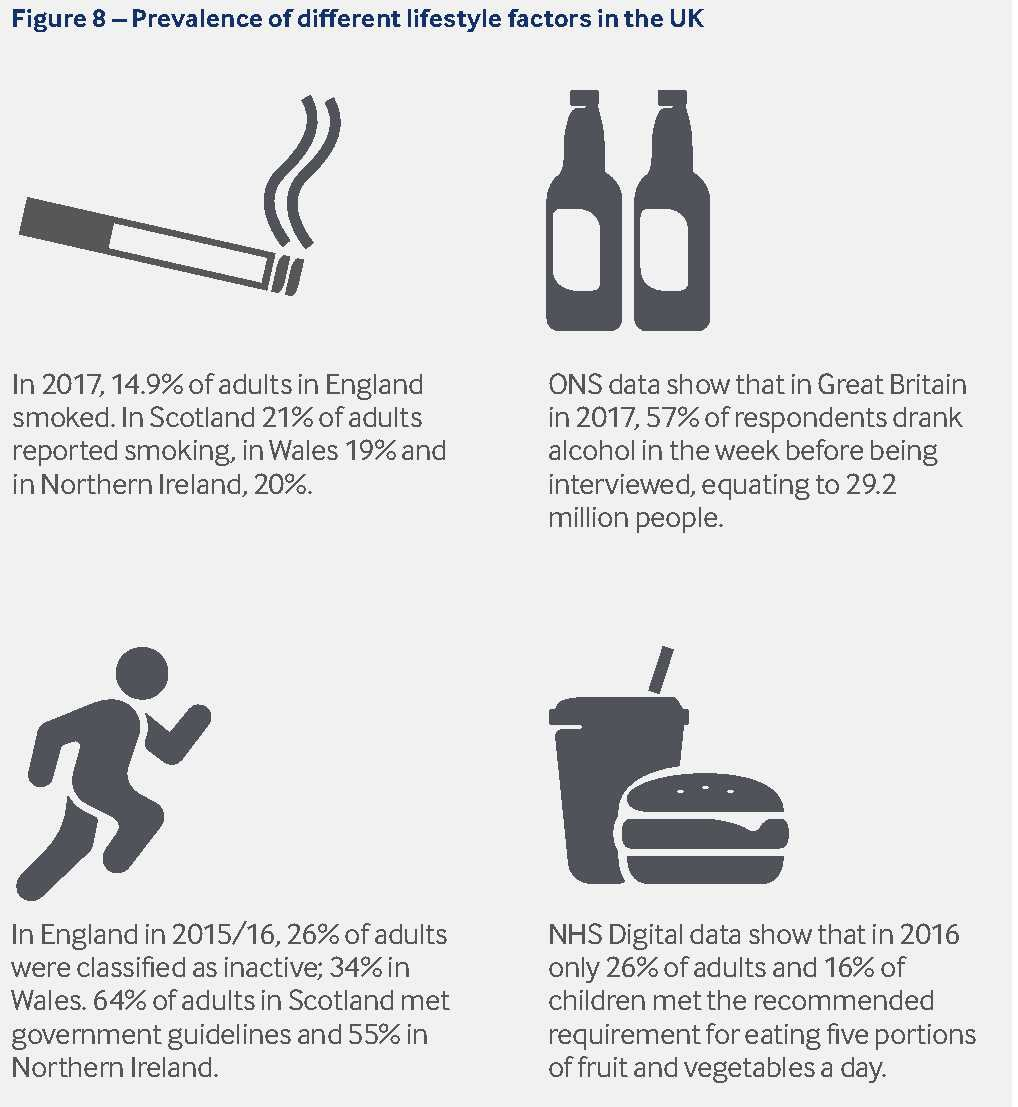
\includegraphics[width=3in]{images/ch3/15.png}
                    \caption{Prevalence of different lifestyle factors in the UK}
                \end{figure} 
            \begin{figure}[H]%option [H] means "strictly here"
                    \centering
                    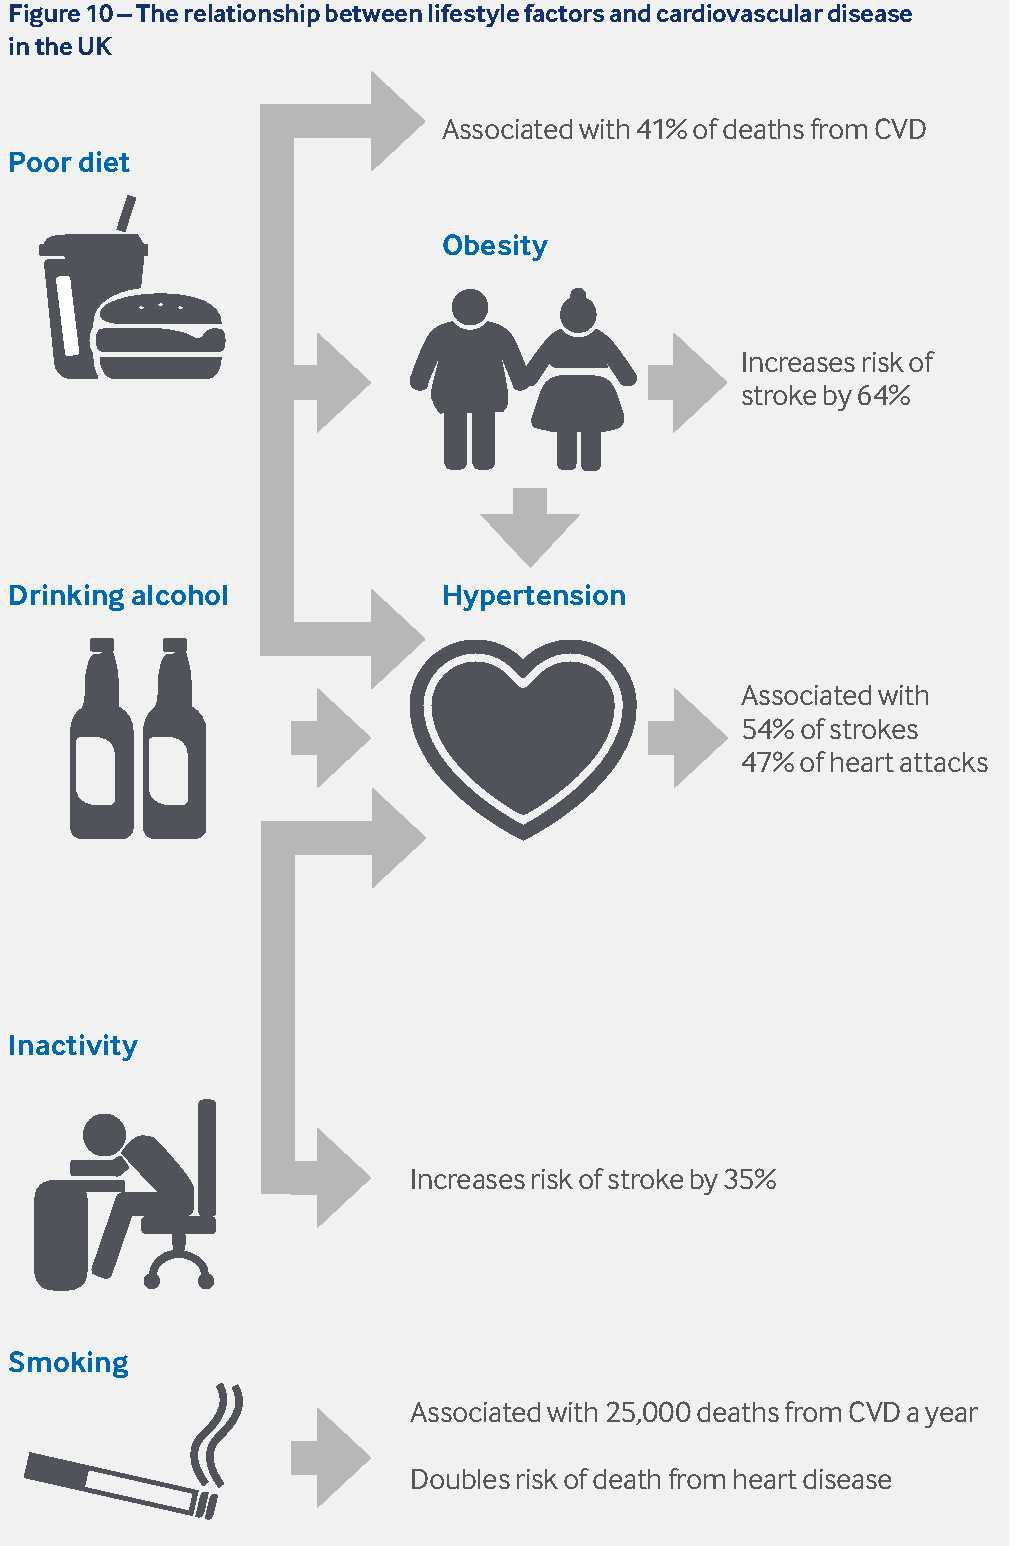
\includegraphics[width=3in]{images/ch3/16.png}
                    \caption{The relationship between different lifestyle factors and cardiovascular diseases in the UK}
                \end{figure} 

\begin{itemize}           
        \item Poor lifestyles, such as poor diet, drinking alcohol, inactivity and smoking, are associated with cardiovascular diseases.
        \end{itemize}

\begin{figure}[H]%option [H] means "strictly here"
                \centering
                \includegraphics[width=5in]{images/ch3/17.png}
                \caption{PAF (Population Attributable Factions) for major risk factors for all-cause YLLs (Years of Life Lost) rate per 100,000 population for England, Scotland, Wales, and Northern Ireland, both sexes, 2016}
            \end{figure} 

\begin{itemize}           
        \item The population attributable fraction is the proportional reduction in population disease or mortality that would occur if exposure to a risk factor were reduced to an alternative ideal exposure scenario. 
        \item The ten leading risk factors contributing to YLLs were similar in rank across the four regions of the UK. Although the ranks were similar, the PAF of each risk factor varied in size in different countries, such as a higher PAF from tobacco in Scotland, and from alcohol and drug use in Scotland and Northern Ireland, compared with the other UK regions.
        \item Poor lifestyles do matter for health, although most money goes to curative health.
        \end{itemize}

        \subsection{How Is the Health Budget Spent?} 
        \subsubsection{Worldwide}
        
            \begin{figure}[H]%option [H] means "strictly here"
                \centering
                \includegraphics[width=4in]{images/ch3/10.png}
                \caption{Total general government expenditure on health as a percentage of GDP, 2020}
            \end{figure} 
        \begin{itemize}           
            \item The biggest share goes to hospital services, followed by outpatient services, so most money is used to treat people in the first place.
        \end{itemize}
        
        \subsubsection{UK}
        \begin{figure}[H]%option [H] means "strictly here"
                \centering
                \includegraphics[width=4in]{images/ch3/18.png}
                \caption{Government healthcare expenditure by share of healthcare providers, UK, 2018}
            \end{figure} 
 \begin{itemize}           
        \item Hospitals and ambulatory healthcare combined accounted for 73 percent of government healthcare expenditure in 2018
        \end{itemize}              

\subsubsection{Preventive care expenditure is easy to cut, UK}
        \begin{figure}[H]%option [H] means "strictly here"
                \centering
                \includegraphics[width=4in]{images/ch3/19.png}
                \caption{Government expenditure on curative or rehabilitative care and long-term care grew, in real terms, every year from 2014 to 2018, index: 2014 = 100}
            \end{figure}
\begin{itemize}           
        \item Preventive care expenditure has decreased since 2015. This is because it is easy to cut. Curative care is difficult to cut, so the expenditure has increased over time.
        \end{itemize} 

        \begin{figure}[H]%option [H] means "strictly here"
                \centering
                \includegraphics[width=4in]{images/ch3/20.png}
                \caption{Public health grant (allocation) VS local government spending (out-turn), real terms}
            \end{figure}
\begin{itemize}           
        \item The blue bars show the total local government spending on healthcare, which increased in 2020/21 due to Covid-19.
        \item The grey line shows the money allocated to public health prevention. It decreased since 2015/16. This is because it is easy to cut. 
        \end{itemize} 
        
        \begin{figure}[H]%option [H] means "strictly here"
                \centering
                \includegraphics[width=4in]{images/ch3/21.png}
                \caption{Local authority public health percentage change in spending since 2015/16 by element of provision, England, 2021/22 real terms (GDP deflator)}
            \end{figure}
\begin{itemize}           
        \item For preventive healthcare expenditure, only obesity for children increased, since it is a major problem for children in the UK and costs NHS a lot of money. The expenditure is cut across all other categories.
        \end{itemize} 

        \subsection{Early Intervention and Prevention}
\begin{itemize}           
        \item Early intervention and prevention approaches aim to support health and wellbeing by taking action before health problems worsen, or by preventing health problems for occurring in the first place. 
        \item Public Health Prevention = improving public health through disease prevention
        a. Clinical interventions such as screening and vaccinations;
        b. Population-level measures aimed at influencing health behaviours or
addressing the social determinants of health (e.g. living conditions, education etc.).
        \item Early Intervention = strategies aimed to mitigate the effects of problems once they have been identified.
        – Some specifically targeted at the ‘early years’, including pregnancy, early parenting and the early parent-child relationship.
        \item A NICE (National Institute for Health and Care Excellence) review of the cost-effectiveness of 200 interventions found that 30 (15 percent) were cost-saving and 141 (70.5 percent) were cost-effective.
        \end{itemize} 

\subsection{Why government intervention in getting people to become healthier?}
        \begin{figure}[H]%option [H] means "strictly here"
                \centering
                \includegraphics[width=4in]{images/ch3/22.png}
                \caption{Views on support for or opposition to public health interventions by the government}
            \end{figure}

\subsubsection{Reasons for government intervention:}          
\begin{itemize}           
        \item improve human capital, increase productivity, raise tax revenue in the future
        \item market failure: asymmetric information (e.g. junk food: consumers don't know the content/how much is going to harm them)
        \item public goods: hospital/public health services, nobody provides unless the government provides, it is expensive
        \item moral hazards
        \item negative externality (smoking)
        \item time-inconsistent preference (procrastination: go to the gym); addictive goods - the government can nudge/remind people
        \item In order to make progress and develop effective policies, we need first to understand how health is produced.
\end{itemize} 


\section{$\star$ The Production of Health as Human Capital: The Grossman Model}

    \subsection{Introduction}
    
        \begin{itemize}
            \item Grossman (1972) studied how individuals allocate their resources to produce health. He combined the theory of human capital and the theory of the allocation of time to explain the demand for health. Health is a unique good. We use time/resources/money to produce it and enjoy it.
            \item Four important aspects
            \begin{enumerate}
                    \item Health can be treated \empha{both as a consumption and an investment good}. As a \emphb{consumption good}, health yields direct utility. As an \emphb{investment good}, health increases the number of healthy days available to participate in the market and non-market activities.
                    \item Health lasts for more than one period. It \emphb{depreciates} (e.g. ageing process; if no vaccine immunity, poorer health; if don't go to the gym, poorer health) and can be analyzed like a capital good.
                    \item Individuals are not passive consumers of health: they produce it, spending time and money (buy market inputs).
                    \item Demand for medical care is derived: people demand medical care not per se, but to produce health.
                \end{enumerate}
            \item As both a consumption and an investment good, optimal health capital accumulation requires the decision-making of its owner – the individual – who is \emph{both the consumer and the producer}.    
        \end{itemize}        

    \subsection{Preferences, Utility, and Death}
    
        Health as a consumption good enters directly into utility. Here, we model an individual's \emphb{Intertemporal Utility Function} as:
        \begin{equation*}
            U = U(\underbrace{\varphi_0 H_0}_{h_0},...,\underbrace{\varphi_n H_n}_{h_n},Z_0,...,Z_n)
        \end{equation*}
        where:
        \begin{itemize}
            \item $H_0$ : inherited stock of health (predetermined)
            \item $H_i$ : stock of health in the $i$th time period
            \item $\varphi_i$ : service flow per unit stock
            \item $h_i$ = $\varphi_iH_i$ : healthy days
            \item $Z_i$ : non-health commodity
        \end{itemize}
        Length of life is \emph{endogenous}: \emphb{death} occurs when $H = H_{min}$. The lifespan is determined by individuals' choices of working time ($TW_i$), time spent on producing health investment ($TH_i$), time spent on producing non-health commodities ($T_i$), and the purchase of other market inputs ($M_i$).
        
        Individuals \emph{maximise their utilities} subject to resource (time/budget) constraints (section \ref{sec:health_res_cons}) and production technologies (section \ref{sec:health_tech_cons}) introduced below.

    \subsection{Two Resource Constraints}\label{sec:health_res_cons}
    
        Here, we have 2 constraints: the budget constraint and the time constraint.

        The \emphb{Budget Constraint} is:
        \begin{equation*}
            \sum_{i=0}^n\frac{P_iM_i+V_iX_i}{(1+r)^i}=\sum_{i=0}^n\frac{W_i \times TW_i}{(1+r)^i}+ A_0
        \end{equation*}
        \begin{equation*}
            \text{PV of Health and Non-Health Commodities} = \text{PV of Labour Earnings} + \text{Initial Assets}
        \end{equation*}
        where:
        \begin{itemize}
            \item $P_i$ : price for health
            \item $V_i$ : price for non-health commodity
            \item $M_i$ : good inputs in the production of health
            \item $X_i$ : good inputs in the non-health commodity
            \item $W_i$ : wage rate
            \item $TW_i$ : time spent working 
            \item $A_0$ : initial assets
            \item $r$ : interest rate
        \end{itemize}
        The \emphb{Time Constraint} is:
        \begin{equation*}
            \underbrace{TW_i+TH_i+T_i}_{h_i} +TL_i= \aleph
        \end{equation*}
        where:
        \begin{itemize}
            \item $TW_i$ : time spent on working
            \item $TH_i$ : time spent on producing health
            \item $T_i$ : time spent on producing other goods we enjoy
            \item $TL_i$ : time loss due to illness
            \item  $\aleph$  : overall time endowment ($\aleph = h_i + TL_i$)
            \item $h_i$ : healthy days ($h_i=TW_i+TH_i+T_i$)
        \end{itemize}    
    
    \subsection{Production Technologies (Production Constraints)}\label{sec:health_tech_cons}
    
        Here, we have 5 production functions in total:

        The \emphb{Healthy Time Production Function} is:
        \begin{equation*}
            h_i=f(H_i)
        \end{equation*}
        which means healthy days can be produced by some technology using health stocks.
        
        The \emphb{Health Stock Production Function} is:
        \begin{equation*}
            H_{i+1}=H_i-\delta_i H_i+I_i
        \end{equation*}
        where:
        \begin{itemize}
            \item $I_i$ : gross investment
            \item $\delta_i$ : depreciation (exogenous, might vary with age, e.g. older, higher depreciation)
        \end{itemize}
        The health stock PF implies that when investment is high, an individual can overcome the high rate of depreciation.

        Such specification brings \emph{two problems}:
        \begin{itemize}
            \item Linearity: It does not account for diminishing marginal returns
            \item It does not account for random shocks
        \end{itemize}

        The \emphb{2 Household Production Functions} are:

        Production of health investment ($I_i$):
        \begin{equation*}
            I_i=I_i(M_i,TH_i;E_i)
        \end{equation*}
        Production of non-health commodities ($Z_i$):
        \begin{equation*}
            Z_i=Z_i(X_i,T_i;E_i)
        \end{equation*}
        where
        \begin{itemize}
            \item $M_i$ = good inputs in the production of health
            \item $X_i$ = good inputs in the production of non-health commodity
            \item $TH_i$ : time spent on producing health
            \item $T_i$ : time spent on producing other goods we enjoy
            \item $E_i$ : stock of human capital (education) $\implies$ better education, better health
        \end{itemize}
        We can see that the production of health and non-health commodities needs both time and money. (Cooking and going to the gym also matter.) 

        The \emphb{Income Production Function} is:
        \begin{equation*}
            Y_i = W_i\times TW_i
        \end{equation*}
           
    \subsection{The Production Possibility Frontier}

        The \emphb{Production Possibility Frontier} shows the frontier of the feasible set of non-health commodities ($Z$) health stock ($H$).

        Since an individual dies and cannot consume/produce any non-health commodities, we must have $Z_i=0$ when $H_i \leq H_{min}$.

        This is a WRONG example:
        \begin{figure}[H]
            \centering
            \includegraphics[width=3in]{images/ch3/23.png}
            \caption{Wrong PPF}
        \end{figure}
        A CORRECT example and \emphb{Optimality}:
        \begin{figure}[H]
            \centering
            \includegraphics[width=3in]{images/ch3/24.png}
            \caption{Correct PPF and the Optimal Point}
        \end{figure}
        We must have $H_{min}$, $Z_{max}$, and $H_{max}$.  We reach the optimal point ($Z^*,H^*$) when the indifference curve is tangent to the PPF. In the following 2 sections, we will explain this is also level of health stock where MEC and COC curves intersect.

    \subsection{MEC and COC Curves}

        The \emphb{Marginal Efficiency of Health Capital (MEC)} curve shows the value of the additional healthy days gained from a 1-unit increase in the health stock (MPH). MEC is the monetary value of the marginal productivity of health stocks. It is diminishing as an individual's health stock expands.

        MEC has the following expression:
        $$MEC=MPH\times w$$
        where:
        \begin{itemize}
            \item $w$: wage rate
            \item $MPH$: marginal productivity of health stock
        \end{itemize}

        The \emphb{Cost of Capital (COC)} curve represents the supply price of capital or the cost of holding an additional unit of health capital. Its position is determined by the depreciation rate of the health stock ($\delta$) and the opportunity cost of holding health capital (r):
        $$COC=r+\delta$$

    \subsection{Optimisation, Demand for Health, and Ageing}

        \subsubsection{Optimisationa and Demand for Health}\label{grossman_demand}
    
            \emphb{Optimality Conditions} for the simplest version of the model:
            \begin{equation*}
                \color{red} \text{PV of the Marginal Cost of Gross Health Investment} = \text{PV of Marginal Benefits of Health}
            \end{equation*}
            We have seen this is the tangent point of the FPF and indifference curve. Meanwhile, this is also the point where the Marginal Efficiency of Health Capital (MEC) curve intersects the Cost of Capita (COC) curve:
            \begin{equation*}
                \color{red} \underbrace{r+\delta}_{MC\ (COC)} = \underbrace{MPH \times w}_{MB\ (MEC)}
            \end{equation*}
            \begin{figure}[H]
                \centering
                \includegraphics[width=3in]{images/ch3/25.png}
                \caption{MEC and COC of Holding Health Stocks and the Optimal Point}
            \end{figure}

        \subsubsection{What Happens as We Age?}
            \begin{figure}[H]
                \centering
                \includegraphics[width=3.5in]{images/ch3/26.png}
                \caption{Optimality and Aging}
            \end{figure}
            The depreciation rate increases ($\delta \to \delta'$) as we age, so the COC shifts upwards to COC', and the optimal level of health stock we can sustain is lower ($H^* \to H^{*'}$).

        \subsubsection{Health Inequality}

            See section \ref{health_ineq_cause}.

    \subsection{Literature Development and Criticisms}
    
        Since 1972, the Grossman model has been the cornerstone for modelling investment in health capital, spurring a great deal of research, extensions, empirical testing and criticism. Grossman himself reviewed the literature many times, e.g. in the 2000 Chapter “The Human Capital Model” in the Handbook of Health Economics.
        
        Some of the main \emphb{criticisms} of the Grossman model:
            \begin{itemize}
                \item It does not preclude an individual choosing to live forever (Ehrlich and Chuma, JPE 1990 “does not determine the length of life")
                \item It does not provide an adequate conceptual framework for the SES (socioeconomic status)-health gradient (Galama and van Kippersluis, EJ, 2018): They develop a model which incorporates health, longevity, wealth, earnings, education, work, job-related physical and psychosocial health stressors, leisure, health investment (e.g. exercise, medical care) and healthy and unhealthy consumption (including housing, neighbourhood social environment).
                \item Not faithful to gerontological models of health deficit accumulation (Strulik).
                \item It does not include an early childhood phase (Heckman, PNAS 2007).
            \end{itemize}
            
        It is a very active area of research, both theoretically and empirically.




\section{Inequalities in Health}\

    Inequalities in health are not random and are associated with characteristics. Poor people are less healthy, maybe because they eat cheaper food and don't know the benefit of doing exercise (less educated). Education is correlated with health.

    More educated  $\to$  Higher income  $\to$  More resources and information

    \subsection{SES Inequalities in BMI Widen over the Lifecycle and across British Cohorts}
    
        \begin{figure}[H]%option [H] means "strictly here"
            \centering
            \includegraphics[width=4in]{images/ch3/27.png}
            \caption{SES Inequalities in BMI Widen over the Lifecycle and across British Cohorts}
        \end{figure}
        \emphb{BMI (Body Mass Index)} is not the best measure of body fitness, since it only includes two dimensions (weight and height), it doesn't take into account fat mass, it doesn't include many diseases such as blindness, it is developed in the West and thus the norms may not apply to other ethnicities. However, BMI is a relatively \emph{simple measure}, and it is correlated with obesity and worse body conditions later in life.
        \begin{itemize}
            \subsubsection{Lifecycle:}
            \item The lines are very close in the beginning, the 1946 cohort starts to diverge at the end of adolescence and keeps diverging as they get older. 
            \item Low SES people have higher BMIs than high SES people as they get older.
            \item For each cohort, BMI generally increases as age increases. 
            \subsubsection{Cohort:}
            \item 2000 cohort has a higher BMI at the young age.
            \item The health inequality (divergence) presents in every cohort, and we are not doing anything to effectively reduce it.
        \end{itemize}       
        
    \subsection{Health inequalities are everywhere}
    
        \begin{itemize}
            \item Researchers have documented inequalities in the distribution of health by socioeconomic status, gender, and ethnicity.
            \item Research on socio-economic inequalities in health in the UK has a long history, together with nice data.
            \item In the early part of the 20th century the British government introduced questions on occupation in the decennial census:
            \item The 1970-1972 Decennial Supplement of occupational Mortality (OCPS) showed that men in social class V (unskilled) were 2.5 times as likely to die before the age of 65 than those in social class I (professional). Children in social class V families were twice as likely to die as those in social class I.
        \end{itemize} 

    \subsection{Landmark Studies in Social Class Inequalities in Health in the UK}

        \subsubsection{Brief Listing}
            \begin{itemize}
                \item \emphb{Black Report (1980)}
                \begin{itemize}
                    \item Health inequalities were widening, the problem had little to do with NHS.
                    \item Four possible explanations: (1) data artefact; (2) social selection (sicker people $\Rightarrow$ less able to study and work $\Rightarrow$ poorer); (3) behaviour; (4) material circumstances.
                    \item Policy recommendation: reduce poverty, spend more on prevention.
                \end{itemize} 
                
                \item \emphb{Whitehead Report (1987)}
                \begin{itemize}
                    \item Commissioned by the Health Education Council (HEC) and headed by
        Margaret Whitehead.
                    \item Health inequalities widened since the Black Report.
                    \item HEC was scrapped: was campaigning on alcohol, tobacco and diet issues which upset some of the government’s financial supporters.
                \end{itemize}
                
                \item \emphb{Acheson Report (1998)}
                \begin{itemize}
                    \item Commissioned by the new Labour (Blair) government in 1997, under the chairmanship of a former Chief Medical Officer, Sir Donald Acheson.
                    \item Similar findings and recommendations as the Black Report: the root cause of inequalities in health was poverty.
                \end{itemize}
        
                \item \emphb{Whitehall I Study}
                \begin{itemize}
                    \item Examined over 18,000 male British civil servants over 10 years, starting in 1967.
                    \item Showed that mortality was higher among those in the lower grade than in the higher grade – for all causes and CHD.
                    \item Controlling for risk factors (smoking, obesity, exercise, blood pressure) accounted for 40 percent of the gradient.
                \end{itemize}
        
                \item \emphb{Whitehall II Study}
                \begin{itemize}
                    \item Examined 10,308 civil servants aged 35-55, 2/3 men and 1/3 women, starting in 1985.
                    \item Showed social gradient for several diseases.
                    \item Added job-related stress to the traditional risk factors for low social class.
                \end{itemize}
        
                \item \emphb{Fair Society, Healthy Lives: The Marmot Report (2010)}
                \begin{itemize}
                    \item Concluded that reducing health inequalities would require action on six policy objectives: number 1 is “Give every child the best start in life”.
                \end{itemize}
        
                \item \emphb{Health Equity in England: The Marmot Review 10 Years On (2020)}
                \begin{itemize}
                    \item “This ‘10 years on’ report shows that, in England, health is getting worse for people living in more deprived districts and regions, health inequalities are increasing  and, for the population as a whole, health is declining. The data that this report brings together also show that for almost of all the recommendations made in the original Marmot Review, the country has been moving in the wrong direction. In particular, lives for people towards the bottom of the social hierarchy have been made more difficult. Some of these difficulties have been the direct result of government policies, some have resulted from failure to counter adverse trends such as increased economic inequalities or market failures.”
                \end{itemize}
            \end{itemize} 

        \subsubsection{The Marmot Review}
            \begin{figure}[H]
                \centering
                \includegraphics[width=4in]{images/ch3/28.png}
                \caption{Life expectancy and disability-free life expectancy (DFLE) at birth, by neighbourhood income level, England, 1999-2003}
            \end{figure}
            \begin{itemize}
                    \item \emphb{Disability-Free Life Expectancy (DFLE)} measures not only how long you live but also how well you live, so there is a gap between life expectancy and DFLE.
                    \item There is a discrepancy in the life expectancy/DFLE between the most deprived and the least deprived people in England.
            \end{itemize} 
        
            \begin{figure}[H]
                \centering
                \includegraphics[width=4in]{images/ch3/29.png}
                \caption{Life expectancy at birth by area deprivation quintiles and sex, England, 2003–05 to 2015–17}
            \end{figure}
            \begin{itemize}
                \item Life expectancy is increased for everyone.
                \item The most deprived has the lowest life expectancy.
                \item The gaps between groups are almost the same as time passed, so inequalities stay the same.
            \end{itemize}
        
        \subsubsection{Public Health England}
            \begin{figure}[H]
                \centering
                \includegraphics[width=5in]{images/ch3/30.png}
                \caption{What causes of death are driving the gap in life expectancy among the most deprived people and the least deprived people, male/female}
            \end{figure}
          In 2014 to 2016, higher mortality rates in more deprived areas from heart disease, lung cancer, and chronic lower respiratory diseases accounted for around a third of the total gap in life expectancy.
        
        \subsubsection{The IFS Deaton Review (2019-)}
            \begin{figure}[H]
                \centering
                \includegraphics[width=4in]{images/ch3/31.png}
                \caption{Life expectancy at birth, England and Wales, 1841-2000, Males/Females}
            \end{figure}
            The life expectancy increased and almost doubled. Females had higher life expectancy. The biggest drop was in World War II.
         
            \begin{figure}[H]
                \centering
                \includegraphics[width=4in]{images/ch3/32.png}
                \caption{Life expectancy at birth, England, 2000-2021, Males/Females}
            \end{figure}        
            The second biggest drop was during the pandemic (about 1 year). 
        
            \begin{figure}[H]
                \centering
                \includegraphics[width=4in]{images/ch3/33.png}
                \caption{Fall in life expectancy by deprivation decile, England, 2019-21}
            \end{figure}        
            During the Covid-19 pandemic, the most deprived male had a life expectancy drop of 1.8 years, while the least deprived male had a life expectancy drop of 0.7 years. Males tend to have a bigger drop than females. 

    \subsection{Why Do Health Disparities Exist?}\label{health_ineq_cause}

        Understanding the causes of health disparities is of key policy importance for addressing them (health subsidies, health information, nudge, for the poor people).
        
        \emphb{Potential Causes} are:
        \begin{enumerate}
            \item \empha{SES can causally affect health}. In terms of the Grossman model (Section \ref{grossman_demand}):
            \begin{itemize}
                \item In the framework of the Grossman model, SES could actually affect health.
                Firstly, people with better SES (e.g. higher education) can have higher Marginal Efficiency of Health Capital (MEC), for instance, due to higher wages:
                $$MEC\uparrow=MPH\times w\uparrow$$
                \item Also, they may have a lower rate of depreciation $\delta$ due to less stress. This will shift down their COC:
                $$COC\downarrow=r+\delta \downarrow$$
                \item Higher MEC, lower COC $\leadsto$ Higher equilibrium health stock
                \item Besides, people with better SES typically have more wealth. Hence, their FPF could be expended compared with disadvantaged people, which also leads to higher health stocks.
            \end{itemize}
            \item \empha{Early health can causally affect SES} (\emphb{Health Selection}).\\
            For example, unhealthy child $\leadsto$ less educated $\leadsto$ lower SES $\leadsto$ poorer adult health
            
            \item \empha{Both can be affected by third factors}.\\
            For example: time preferences (Fuchs’ hypothesis): people who are willing to delay gratification will invest more in both health and education.
        \end{enumerate}

\section{Education and Health: Causal Inference}

    \subsection{Observed Difference in Health by Education (Compulsory vs. Post-Compulsory)}
    
        \begin{figure}[H]
            \centering
            \includegraphics[width=4in]{images/ch3/34.png}
            \caption{Disparities by Education (compulsory vs. post-compulsory)}
        \end{figure}    
         The graph shows the raw differentials in the outcomes between individuals with post-compulsory and compulsory level of education.          Individuals with post-compulsory education tend to have better health.

    \subsection{Causality or Correlation? An Overview of Empirical Strategies}
    
        Key question: \empha{Is the positive correlation between health and schooling causal?}
        
        Literature has used different approaches to establish causality:
        \begin{itemize}
            \item First set of studies: used \emphb{instrumental variables} with questionable instruments for education (e.g. quarter of birth), finding \empha{strong effects}.
            \item Second set of studies: exploited \emphb{features of the educational system}:
            \begin{itemize}
                \item Lleras-Muney (RevStud, 2005) uses compulsory school and child labour laws in thirty states from 1915 to 1939 as instruments for education and finds a \empha{significant effect in reducing mortality} (using \emphb{DiD}).
                \item Clark and Royer (AER, 2013) use regression discontinuity methods (\emphb{RDD}) exploiting two changes to British compulsory schooling laws and find \empha{no effects on mortality or other measures of health} (discussed in detail in Section \ref{clark_royer_RDD}). Similar results in a recent paper by Janke, Johnston, Propper et al. (JHE, 2018).
            \end{itemize}
            \item Third set of studies: \emphb{twin differences} (different between twins, NOT DiD!) (Lundborg, JPopEc 2013). It suggests that \empha{completing high school improves health, but additional schooling does not lead to additional health gains}. Controlling for certain early life factors that may vary within twin pairs does not alter the main conclusions. Discussed in detail in Section \ref{lundborg_twin_diff}.
            \item Fourth set of studies: more “\emphb{structural}” models: Conti et al., 2010a,b show that \empha{education has a causal component in most outcomes, but with dramatic heterogeneity}; Heckman et al., 2018 sets up a dynamic model and show that \empha{completing high school is especially effective}. See section \ref{sec:structual_health}.
            \item Recent literature: disagreement still exists. See section \ref{sec:health_edu_recent}.
            \item Summary: Grossman (NBER wp 21609, 2015) “The Relationship between Health and Schooling: What’s New?” concludes “There is enough \empha{conflicting evidence} in the studies that I have reviewed to warrant more research on the question of whether more schooling does in fact cause better health outcomes.”
        \end{itemize}

    \subsection{Clark and Royer: RDD (AER, 2013)}\label{clark_royer_RDD}
    
        \subsubsection{Setup}
            \begin{figure}[H]
                \centering
                \includegraphics[width=5in]{images/ch3/35.png}
                \caption{Years of Full-Time Education by Quarter of Birth}
            \end{figure}
            This figure presents data at the quarter-of-birth level using Health Survey of England data. We study how the introduction of \emphb{two compulsory schooling laws} affected the fraction of cohorts with stated \emphb{amount of education}:
            \begin{itemize}
                \item The first reform took effect on April 1, 1947, which increased the compulsory school leaving age from 14 to 15.
                \item the second took effect on September 1, 1972, which increased the compulsory school leaving age from 15 to 16.
            \end{itemize}
            The vertical lines are cutoffs corresponding to the first cohorts subject to the new compulsory schooling laws. Since the two compulsory schooling reforms affected 14 (first reform) and 15 (second reform) years old, the first cohorts impacted are those born in April 1933 for the first reform and September 1957 for the second reform.
                     
            The 1947 change reduced the fraction that completed nine years or less by roughly one half; the 1972 change decreased the fraction that completed ten years or less by roughly one quarter. Hence, the reforms did increase students' years of education and reduce the number of students who dropped out at a particular age.

        \subsubsection{Nature of Discontinuity}
            \begin{figure}[H]
                \centering
                \includegraphics[width=5in]{images/ch3/36.png}
                \caption{The Impact of the Compulsory Schooling Changes on Educational Attainment}
            \end{figure}
            
            Here, our \empha{running variable is the year of born (cohorts)}: at certain years of born, there are \empha{``jumps'' in average years of education}.
    

        \subsubsection{Outcomes}

            \begin{figure}[H]
                \centering
                \includegraphics[width=4in]{images/ch3/37.png}
                \caption{The Impact of the Compulsory Schooling Changes on Mortality}
            \end{figure}

            \empha{Outcome variable 1: Mortality}: The two compulsory schooling laws have no effect on mortality (no discontinuity).
     
            \begin{figure}[H]
                \centering
                \includegraphics[width=4in]{images/ch3/38.png}
                \caption{The Impact on Reporting Being in Fair or Worse Health in the 2001 Census}
            \end{figure}  
            
            \empha{Outcome variable 2: Health Fair/Bad or Long-standing Illness}: The reforms cause no change in health fair or bad and long-standing illness.


            \begin{figure}[H]
                \centering
                \includegraphics[width=4in]{images/ch3/39.png}
                \caption{Prevalence of Chronic Conditions for Months-of-Birth around the ROSLA Reform Cutoff}
                \label{fig:rosla_plot}
            \end{figure} 

            \empha{Other outcome variables}: Another recent paper analysed the same reform and showed that only the prevalence of cardiovascular diseases was affected by the reform.

        \subsubsection{Conclusion}
            \empha{Higher education attainment shows nearly no effect on health conditions (at least at the cutoff).}

        \subsubsection{Extension: What If We Run an OLS?}
            \begin{figure}[H]
                \centering
                \includegraphics[width=5in]{images/ch3/40.png}
                \caption{ROSLA Reform Estimates}
            \end{figure}        
            If we directly run an OLS regression of education on health, we can see significant correlations. However, if we use 2SLS (Fuzzy RDD), we see that the coefficients are close to 0.

    \subsection{Lundborg, Journal of Population Economics 2013: Twin Differences}\label{lundborg_twin_diff}
        
        The usual setup in twin studies:

        \[ Y_i = \alpha_0+\alpha_1 eduyrs_i+\alpha_2 X_i+\eta_i \]
        
        where  $Y_i$ is certain health outcome.
        
        Take the difference between twins' outcomes:
        
        \[ \Delta Y = \beta_0+\beta_1\Delta eduyrs+\beta_2 \Delta X+\Delta \eta \]
        where  $\Delta Y=Y_i-Y_j$ 
        
        This is a fixed-effect regression, which eliminates effects of common characteristics between twins.
        
        However, $\beta_1$ cannot not be interpreted as the causal effect of education on health, as education is subject to selection and is likely to be correlated with the error term (endogeneity: ability/effort/parents' investment), so we still need an instrument for $\Delta eduyrs$.
        
        To address this concern, Lundborg exploits the unusually rich MIDUS data and examine to which extent his results are robust to controlling for differences in early life factors, such as parental treatment, \empha{within twin pairs}.

        Lundborg concludes that \empha{completing high school improves health}, as measured through self-reported health, chronic conditions, and exercise behavior, but that \empha{additional schooling does not lead to additional health gains}. Controlling for certain early life factors that may vary within twin pairs does not alter the main conclusions.


    \subsection{Explaining/Decomposing the Education-Health Gradient}

        \subsubsection{Cutler and Lleras-Muney (JHE, 2010)}

            \begin{itemize}
                    \item Cutler and Lleras-Muney (JHE, 2010) examine possible explanations for the relationship between education and health, using several datasets from US and UK. They use OLS regression and see \empha{how much of the coefficient goes down when adding additional covariates}.
                    \item They are able to explain two-thirds of the gradient.
                    \item "Economic resources" is able to explain 32 percent of the gradient. "Specific knowledge" is able to explain 12 percent of the gradient (US dataset). "Cognitive ability" seems to explain a lot in the UK dataset. "Tastes" and "Personality" explain a little and "social integration" explains somehow.
            \end{itemize}
            \begin{figure}[H]%option [H] means "strictly here"
                \centering
                \includegraphics[width=4in]{images/ch3/41.png}
                \caption{Share of education gradient explainable by different factors}
            \end{figure}
                
        \subsubsection{Conti and Hansman (JHE, 2013)}

            \begin{itemize}
                \item Conti and Hansman (JHE, 2013) test the robustness of Cutler and Lleras-Muney's (CLM) results by using alternative measures of child personality available in the National Child Development Study:
                    \begin{itemize}
                        \item the Rutter Behavior Scale (ages 7, 11 and 16)
                        \item the British Social Adjustment Guide (BSAG, ages 7 and 11):
                    \end{itemize}
                \item CLM results show that adult personality explains very little of the education-health gradient, but Conti and Hansman (JHE, 2013) show that child personality contributes the education-health gradient to an extent nearly as large as cognition. 
                \item \empha{Childhood matters.}
            \end{itemize}

            \begin{figure}[H]
                \centering
                \includegraphics[width=4in]{images/ch3/42.png}
                \caption{How much education-health gradient is explained by cognition, personality and motivation}
            \end{figure} 

            \begin{figure}[H]
                \centering
                \includegraphics[width=4in]{images/ch3/43.png}
                \caption{Decomposition of the Education-Health Gradient}
            \end{figure} 

            Non-cognitive factors such as externalising and motivation are at least as important as cognition in explaining the gradient.

    \subsection{Structural Models in Education-Health Gradient Decomposition}\label{sec:structual_health}
        
        \subsubsection{The Early Origins of the Gradient: Conti, Heckman et al. (AER, PPS, 2010a,b)}

            \begin{itemize}
                \item Conti, Heckman et al. (AER, PPS, 2010a,b) \empha{decompose observed educational differentials into causal components of education and components due to selection on early childhood human capital}. 
                \item In their framework, early childhood factors affect health both through education and directly. Both channels are quantified.
                    \begin{itemize}
                        \item They estimate a semiparametric structural model of the choice of schooling (decision to stay on at 16) and the causal effect of schooling on a variety of outcomes at age 30:
                        \begin{itemize}
                            \item labour market (wages and employment)
                            \item health status (self-reported health, depression and obesity)
                            \item health behaviours (smoking, exercise)
                        \end{itemize}
                        \item Three childhood (age 10) endowments:
                        \begin{itemize}
                            \item cognition (e.g. British Ability Scales)
                            \item noncognitive traits (e.g. locus of control)
                            \item health (height, head circumference)
                        \end{itemize}    
                    \end{itemize}
                \item They look at the mean effect of education on health (like previous literature) and also at heterogeneity in treatment effects for people with different early childhood endowments.
                \item Data: British Cohort Study (BCS70), a cohort of all individuals born in one week of April 1970 in the United Kingdom.
            \end{itemize}
            
            \empha{Outcomes:}
            \begin{itemize}
                \item Causal component of education and effects of childhood characteristics: \empha{educations and early childhood characteristics both have causal effects on most of the outcomes.}
                    \begin{figure}[H]%option [H] means "strictly here"
                        \centering
                        \includegraphics[width=4in]{images/ch3/44.png}
                        \caption{How education and early life factors share the causal effects on different health outcomes}
                    \end{figure}
                \item Specific Outcomes
                \begin{itemize}
                    \item Obesity
                        \begin{figure}[H]%option [H] means "strictly here"
                            \centering
                            \includegraphics[width=4in]{images/ch3/46.png}
                            \caption{The Effects of Childhood Endowments on the Probability of being Obese at Age 30}
                        \end{figure} 
                        Cognition matters little. Non-cognitive explains a little bit. Early physical health is the most important determinant of obesity.
                    \item Smoking
                        \begin{figure}[H]%option [H] means "strictly here"
                            \centering
                            \includegraphics[width=4in]{images/ch3/45.png}
                            \caption{The Effects of Childhood Endowments on the Probability of being a Daily Smoker at Age 30}
                        \end{figure} 
                        Cognition doesn't affect smoking. Non-cognitive factors (e.g. self-regulation and motivation) and physical health are equally important determinants of smoking.
                        \begin{figure}[H]%option [H] means "strictly here"
                            \centering
                            \includegraphics[width=4in]{images/ch3/47.png}
                            \caption{Heterogeneity in the Effects of Education on Smoking}
                        \end{figure} 
                        \empha{Effects of education on smoking is heterogeneous}: beneficial effect of education is much bigger at the top of the cognitive ability distribution
                \end{itemize}
            \end{itemize}

        \subsubsection{Evidence from a Dynamic Model: Heckman, Humphries and Veramendi (JPE 2018)}

            \begin{figure}[H]%option [H] means "strictly here"
                \centering
                \includegraphics[width=5in]{images/ch3/48.png}
                \caption {Evidence from a Dynamic Model}
                \end{figure}

            Heckman, Humphries and Veramendi (JPE 2018) extend the structural framework discussed above into a dynamic model of schooling choice and estimate causal effects from multiple levels of schooling. They find \empha{substantial continuation value of schooling for high-ability individuals, but not for low ones beyond high school.}

            \begin{itemize}
                \item The figure shows how additional level of education affects wages and health compared to previous education level
                \item The black bars labelled “Observed” are the raw differences found in the data, and the gray bars are estimated causal components.
                \item The estimated average causal effects are the highest for high schools.
            \end{itemize}
         
    \subsection{The State of the Literature}\label{sec:health_edu_recent}

        \begin{itemize}
            \item Recent review “The Effect of Education on Health and Mortality: A Review of Experimental and Quasi-Experimental Evidence” by T. Galama, A. LlerasMuney, H. van Kippersluis, Oxford Research Encyclopedia of Economics and Finance (2018):
                \begin{itemize}
                    \item “There is no convincing evidence of an effect of education on obesity, and the effects on smoking are only apparent when schooling reforms affect individuals’ track or their peer group, but not when they simply increase the duration of schooling.”
                    \item “An effect of education on mortality exists in some contexts but not in others, and seem to depend on: (a) gender; (b) the labour market returns to education; (c) the quality of education; (d) whether education affects peers’ quality.”
                \end{itemize}
            \item Important step forward would be to understand the quality and content of further education, years beyond the minimum school leaving age, and both short-, medium-, and long-term outcomes.
            \item Some papers analyse the \emphb{publication bias} towards the positive effects of education on health.
        \end{itemize}

    \subsection{Where Next?}

        \begin{itemize}
            \item Grossman (NBER wp 21609, 2015) “The Relationship between Health and Schooling: What’s New?” concludes “There is enough \empha{conflicting evidence} in the studies that I have reviewed to warrant more research on the question of whether more schooling does in fact cause better health outcomes.”
            \item Among promising areas of current and future research:
            \begin{itemize}
            \item Does schooling quality matter?
            \item What are the mechanisms via which schooling influences health and health behaviours?
            \item What is the role of genes?
            \item What is the role of subjective expectations of returns?
            \end{itemize}
        \end{itemize}

\clearpage










\section*{Bibliography}

    \begin{itemize}
        \item Barcellos et al. (2018). PNAS. Education can reduce health differences related to genetic risk of obesity.
        \item Clark, D. and Royer, H. (2013). The Effect of Education on Adult Mortality: Evidence from Britain. American Economic Review, 106(6),
        2087-2120.
        \item Conti, G., and Hansman, C. (2013). Personality and the education–health gradient: A note on “Understanding differences in health
        behaviours by education”. Journal of health economics, 32(2), 480-485.
        \item Conti, G. and Heckman, J.J. (2010). Understanding the Early Origins of the Education-Health Gradient: A Framework That Can Also Be Applied to Analyze Gene-Environment Interactions. Perspectives on Psychological Science, 5(5), 585-605.
        \item Conti,G., Heckman,J.J. and Urzua, S. (2010).The Education-Health Gradient. American Economic Review P P, 100(2), 234-238.
        \item Cutler, D. M., and Lleras-Muney, A. (2010). Understanding differences in health behaviours by education. Journal of health economics,
        29(1), 1-28.
        • [Erlich, I., and H. Chuma (1990) “A model of the demand for longevity and the value of life extensions”, Journal of Political Economy
        98:761-782.]
        \item Galama,T. and H. van Kippersluis (2018).A Theory of Socioeconomic Disparities in Health Over the Life Cycle, Economic Journal.
        \item Galama, Titus J. and Lleras-Muney, Adriana and van Kippersluis, Hans, The Effect of Education on Health and Mortality: A Review of
        Experimental and Quasi-Experimental Evidence, Oxford Encyclopedia of Economics and Finance.
        \item Gilleskie, D. (2008). Health Capital: Theory and Empirical Evidence. Incentives and Choice in Health Care MIT Press: Cambridge, MA.
        \item Grossman, M. (1972). On the concept of health capital and the demand for health. Journal of Political economy, 80(2), 223-255.
        \item Grossman, M. (2000). The human capital model. Handbook of health economics, 1, 347-408.
        \item Grossman, M. (2015).The Relationship between Health and Schooling: What’s New? NBER wp 21609.
        \item Heckman, J. J. (2007). The economics, technology, and neuroscience of human capability formation. Proceedings of the national
        Academy of Sciences, 104(33), 13250-13255.
        \item Heckman, J.J., J.E. Humphries and G. Veramendi (2018). Returns to Education: The Causal Effects of Education on Earnings, Health
        and Smoking. Journal of Political Economy, October S1.
        \item Janke, K., D.Johnston, C. Propper and M. Shields (2018).The Causal Effect of Education on Chronic Health Conditions. IZA DP 11353.
        \item Lleras-Muney, A. (2005). The relationship between education and adult mortality in the United States. The Review of Economic
        Studies, 72(1), 189-221.
        \item Lundborg, P. (2013).The health returns to schooling—what can we learn from twins? Journal of population economics, 26(2), 673-701 
    \end{itemize}
   \chapter{The Health Effects of Early Interventions}

\fancyhead[L]{ECON0024}
\fancyhead[C]{Ch.4 The Health Effects of Early Interventions}
\fancyhead[R]{Kaicheng Lu}
\fancyfoot[L]{\hyperlink{tableofcontents}{Back to Table of Contents}}
\fancyfoot[R]{Kaicheng Lu}
 
\section{Questions we are interested in and motivation}

    \begin{itemize}
        \item We saw the substiantial SES-health gradient last time
        \item Moreover, \href{https://www.sciencedirect.com/science/article/pii/S0047272720300359}{Attanasio, Blundell. Conti and Mason (2019)} showed that this inequality is multidimentional. Inequality in socio-emotional skills (mental health) of 5 year olds has also widened over time.
        \begin{itemize}
            \item  The score on various socio-emotional skills were normalised to 0 for the 1970 cohort, and we can see from figure \ref{SMinequality} that kids born to more educated mothers are better off in 2000 compared to 1970 (gap became bigger).
            \item Interpreting the fig: externalising = social skills; internalising = the ability to focus; higher value is better
        \end{itemize}
        \begin{figure}[H]%option [H] means "strictly here"
            \centering
            \includegraphics[width=13cm]{images/ch4/socioemotional inequality.png}
            \caption{inequality in socio-emotional skills}
            \label{SMinequality}
        \end{figure}
        \item What should we do?
        \begin{itemize}
            \item Try to look at the forgotten aspect in the Grossman health production model: early childhood development
            \item From the data, about a half of the difference in labour market outcomes, health behaviour and health at age 30 can be explained by early life factors happening before $\leq$ 10 years old, and the rest is explained by the causal effect of edu \href{https://www.nber.org/system/files/working_papers/w18466/w18466.pdf}{(Conti and Heckman, 2010)}
            \item Traits of health inequality also begin early in life: high value of C-Reactive Protein (a measure of inflammation) was documented at mid-40s for those in low SES. At the same time, a similar gradient occurred in childhood, where children born to lower SES households are also more likely to have low birth weight \href{https://www.nber.org/system/files/working_papers/w18466/w18466.pdf}{(Conti and Heckman, 2010)}
             \item SES-health gradient can occur before birth! The fact that the mother resides in deprived neighbourhoods had a significant negative effect on the size of fetus along different dimensions \href{https://www.econstor.eu/bitstream/10419/200319/1/1047143135.pdf}{(Conti et al., 2018)} 
            \begin{figure}[H]%option [H] means "strictly here"
                \centering
                \includegraphics[width=13cm]{images/ch4/Prebirth gradient.png}
                \caption{SES-health gradient before birth}
                \label{Prebirthgradient}
            \end{figure}
            \item This means that the fetuses of poorer moms are smaller, so you will have smaller babies as gestation continues.
            \item The key takeaway from all these stories is that when the kid is conceived, there are already inequalities that will be carried over throught the lifecycle
        \end{itemize}
    \end{itemize}
    
    \textbf{OK maybe it makes sense to start early!} 


\section{Understanding the causal effect of early life conditions}

    \begin{itemize}
        \item The way to look for causal effects involves techniques in labor (quasi-natural experiments from exposure to war, pandemics, policies) and twin-based designs (twin FE, how does the outcome of the high-birth-weight twin look like?)
        \item Here, we look at effect of early childhood conditions on later life outcomes by  exploiting policy shocks and RCTs
        \item A slight detour before studying effect of various internventions: some major findings in the literature on this topic:
        \begin{itemize}
            \item The effect of early shocks are heterogeneous, and the heterogeneity is endogenous. Effect of shocks depends on child endowments, resource constraints and production technologies
            \item Limited understanding on effect of multiple shocks, and the relative importance of biology and behavioural mechanisms
        \end{itemize}
        \item Nevertheless, we should intervene becuase there are frictions preventing parental investment in human capital in early years, such as...
        \begin{itemize}
            \item Information and liquidity constraint
            \item Behavioral factors: Time inconsistency, altruism, cognitive constraints, aspirations
        \end{itemize}
        \item Interventions may help: fetus of smoking moms' are much smaller. A slight caveat here is that higher obesity in the population can lead to too big fetuses (bigger $\neq$ better).
    \end{itemize}


\section{We should intervene. But intervene how?}

    \subsection{Pre-natal Interventions: Home visiting (HV)}
    
        \subsubsection{Nurse Family Partnerships (NFP)}
        
            \begin{itemize}
                \item A program very popular in the USA
                \item Nurses going to houses of first-time low-SES mothers at early stage of pregnancy until the child is 2 years old
                \item Max. 64 visits that provide information and support
                \item Super high return ($\approx$ 500\%)
                \item Treated kids (those with parents being allocated to NFP group) turned out better in terms of better cognition, higher likelihood to graduate high school with honours, less disabilities, and the mothers spent less money in welfare compared to the control group (those with parents allocated to not-that-good usual care system)
                \item Details on cost-saving (\href{https://publications.aap.org/pediatrics/article/144/6/e20183889/77004/Prenatal-and-Infancy-Nurse-Home-Visiting-Effects}{Olds et al., 2019}):
                \begin{figure}[H]%option [H] means "strictly here"
                    \centering
                    \includegraphics[width=13cm]{images/ch4/NFP cost saving.png}
                    \caption{Cost saving in NFP (NV) group}
                    \label{Prebirthgradient}
                \end{figure}
                \textbf{So NFP effective and saves money for the government? We cannot say that until we consider what will happen if we scale this up!}
            \end{itemize}
            
        \subsubsection {Scaling up}
        
            \begin{itemize}
                \item This is a relatively new area of research, and we have relatively good evidence on the effect of HV at scale from Scandinavian countries due to their ``welfare state" setup
                \item \href{https://www.aeaweb.org/articles?id=10.1257/app.20150087}{Hjort et al. (2017)} studied a HV program that was implemented at scale in Denmark from 1937-49
                \item They found that kids in treated areas saw huge improvements in SES and health compared to the control group (note that this effect is for every child in Denmark!)
                \item Some examples of improvement:
                \begin{itemize}
                    \item Children in treated areas more likely to survive after 64 years old
                    \item Less likely to be diagnosed with diseases
                    \item Fewer nights spent in hospitals
                \end{itemize}
            \end{itemize}
            
        \subsubsection{That's Great! But the effect of HV in the UK is unknown due to data problems...}
        
            We also have similar programs in the UK called the Healthy Child Programme (HCP) that ...
            \begin{itemize}
                \item provided advice \& support (e.g.immunization, examination of the child)
                \item Identified risks (e.g. abuse)
                \item Referral to social services if needed
            \end{itemize}
            \textbf{Is it effective? We don't know because there is no data!}
            \\ \\
            However, this program is now facing its own problems
            \begin{itemize}
                \item Massive defunding after Oct 2015 \& local authorities taking over this responsibility
                led to caseload of $>$500 in some regions
                \item Health visitors were moved to the frontline during 
                \item The effect of this is by no means trivial. A survey of visitors by \href{https://discovery.ucl.ac.uk/id/eprint/10106430/8/Conti_Dow_The%20impacts%20of%20COVID-19%20on%20Health%20Visiting%20in%20England%20250920.pdf}{Conti and Dow (2020)} showed that they are concerned about domestic abuse \& violence, parents' mental health, child growth/ development, ...
            \end{itemize}

        \subsubsection{Does the success of the NFP generalise? Investigation of the Family Nurse Partnership (FNP) programme in the UK}
        
            \begin{itemize}
                \item Note the difference between the UK FNP and the US NFP :)
                \item Eligibility criteria of FNP: teenage first-time mom (regardless of SES)
                \item This program was scaled up after being implemented in small scale (10 sites) and received positive feedback
                \item Result of an RCT that came out in 2014 showed that this program did not impact the primary outcomes. However, it improved other outcomes such as child cognitive \& language development, but they were considered secondary. Primary outcomes are health-based, see figure \ref{FNPgoal} for details on the outcomes of interest.
                \begin{figure}[H]%option [H] means "strictly here"
                \centering
                \includegraphics[width=10cm]{images/ch4/OutcomesInterest_FNP.png}
                \caption{Primary and Secondary outcomes in the UK FNP}
                \label{FNPgoal}
                \end{figure}
                \item Follow-up studies showed that the effect on cognitive development (reading and writing) persisted, but there was no impacts on child maltreatment
                \item \textbf{Overall, the program only improved certain aspects of child development, not others.} ``Adding FNP to the usually provided health and social care provided no additional short-term benefits to our primary outcomes"
            \end{itemize}
        
        \subsubsection{What could explain the poor generalizability of the evidence?}
            \begin{itemize}
                \item Difference in culture leading to different behaviour
                \item Difference in trust in public institutions
                \item Difference in counterfactual. The control group gets much worse treatment in the US compared to the UK (remember that control group in the UK gets HV!).
                \begin{itemize}
                    \item In FNP, households get about 39 visits. In control (HV), households get about 16 visits from NHS health visitors
                    \item FNP and HV can both tell mothers about how to make the kid healthy (breastfeeding, not smoking, ...). However, the unique thing about the FNP was that they told moms how to approach child cognitive development (e.g. play with the child)
                \end{itemize}
            \end{itemize}
            \textbf{Note that the secondary outcomes are still important, and the FNP does have a positive significant impact on child development at 5 \& 7 years old.}\\ \\
            \textbf{Also note that recent studies \href{https://jamanetwork.com/journals/jama/article-abstract/2793825?casa_token=hmQ4aJAMtL8AAAAA:22C4Pg2uXeayMj306ws_iqVE56LIoViTQfKUWIhJoXNQ4S9YLAZofvhEgmKVeFYWdOQ3800Tcj4}{(McConnell et al. 2022)} evaluating the effect of the US NFP found that it no longer brings significant improvements on `` maternal and newborn health primary or secondary outcomes". The effectiveness of programs can also change over time even for the same country due to different counterfactuals} 

    \subsection{Post-natal Interventions}
    
        \subsubsection{The Carolina Abecedarian Project}
            \begin{itemize}
                \item This is a small-scale randomised experiment in the US in the 1970s
                \item Send poor African-American kids to intensitve daycare from 0-5 years old
                \item What do they have at the daycare centres?
                \begin{itemize}
                    \item Cognitive and behavioural stimulations
                    \item Healthcare
                    \item Nutrition (food provision)
                \end{itemize}
            \item It is also very effective!
            \begin{itemize}
                \item Benefit-to-Cost Ratio = 7.3
                \item Group exposed to this treatment had better health in adulthood compared to the control
                    \begin{figure}[H]%option [H] means "strictly here"
                \centering
                \includegraphics[width=8cm]{images/ch4/CAP_eval.png}
                \caption{Improved health in adulthood (35 yr old)}
                \label{CAP_eval}
                \end{figure}
            \end{itemize}
            \end{itemize}
            
        \subsubsection{Effect of implementing this at a larger scale: an examination of the effects of Head Start and Sure Start}
            \textbf{Head Start (US)}
            \begin{itemize}
                \item A compensatory preschool program in the US providing head start centres (centres providing a variety of services as in the CAP ) to low income children 
                \item \href{https://www.aeaweb.org/articles?id=10.1257/pol.6.4.135}{Carneiro and Ginja (2014)} found that ``participation in the program reduces the
            incidence of behavioural problems, health problems, and
            obesity of male children at ages 12 and 13; lowers depression
            and obesity among adolescents, and it reduces engagement in
            criminal activities and idleness for young adults."
                %shows that in spite of the lack of program impacts by first grade, there are important longer term impacts of Head Start on the health and criminal behavior of adolescents and young adults
                \item They employed a fuzzy RDD design using discontinuities
            in the probability of participation induced by program eligibility
            rules (note that a jump was only observed in males)
            \item Results in more detail: 
                    \begin{figure}[H]%option [H] means "strictly here"
                \centering
                \includegraphics[width=11.5cm]{images/ch4/HSeval.png}
                \caption{Head Start reduces overweight, behavioural (BPI) and other problems for adolescents}
                \label{CAP_eval}
                \end{figure}
            \end{itemize}
            \textbf{Sure Start (UK)}
            \begin{itemize}
            \item This is a program launched in  1999 in England that was initially targeting diadvantaged communities but then scaled up
            \item The program intends to provide all the help possible to parents in one go
            \begin{itemize}
                \item Provision of health information 
                %via health visitors clinics and will refer to health services if needed
                \item Referral to health services
                \item Stay-and-play, parenting programmes (e.g. FNP)
                \item Parental support, job search assistance
            \end{itemize}
            \item The impact of this program is studied under the following framework:
            $$D^{ya}_{sql(d)}=\delta^{ya}SS_{dq}+\beta^{ya}X_s+\alpha^{ya}Pop_{al}+\gamma^{ya}_q+\pi^{ya}_{l(d)}+\epsilon^{ya}_{sql(d)} $$
            Where
            \begin{itemize}
            \item $D^{ya}_{sql(d)}$: an indicator for whether there is any hospitalization of type y at
        age $\alpha$ for children of sex s born in quarter q and residing in neighborhood l (of LA d)
        \item  $SS_{dq}$: the average number
        of centers per thousand children aged 0-4 that were open between the child’s birth and the age at
        which the outcome is measured
        \item Gender, size of population in the LAs are controlled for
        \item Also included chort of birth \& neighbourhood FEs
        \end{itemize}
        \item Results
        \begin{itemize}
            \item Sure Start reduces overall hospitalisations. Note that there was an increase in hospitalisation at the age of 1, and this is probably due to hospitalisation for preventative purposes
            \begin{figure}[H]%option [H] means "strictly here"
                \centering
                \includegraphics[width=7cm]{images/ch4/SS_overall.png}
                \caption{Sure Start reducing overall hospitalisation}
            \end{figure}
        \end{itemize}
        \item If we decompose by causes of hospitalisation and the extent to which treated areas are deprived
        \begin{figure}[H]%option [H] means "strictly here"
            \centering
            \includegraphics[width=13cm]{images/ch4/SS_bycauseandregion.png}
            \caption{Decomposition of the effect of Sure Start}
        \end{figure}
        \begin{itemize}        
            \item Greater access to Sure
            Start substantially increases hospitalisations for infectious illnesses in infancy, which can be because of referral effects or the spreading of the infectious disease in the childcare centres
            \item However, there are significant and substantial falls in hospitalisations because they build up a
            stronger immune response. This effect fade out in the longer term as the other kids' immune systems catch up after school
            \item Less hospitalisation due to external causes at early ages. Kids are able to fight with each other as they grow older
            \item Big reduction in hospitalisation for mental health at age of 12-13
            \item The program is more effective in poorer areas (poor = green; rich = light blue; middle = pink)
        \end{itemize}
    \end{itemize}

    
\section{Why do these programs work?}
This will help us understand the generalisability of programs implemented in one country at one time\\ \\
\textbf{How early interventions affect us later?}
\begin{itemize}
\item A stylised way
\begin{itemize}
    \item Health is a component of human capital, and good health will yield multiple returns later in life (e.g. education, earnings,...)
    \item Health can be developed throughout the lifecycle by human capital development (think about the factors involved in the production of health) and \textbf {\large{investments}} by parents and governments. Investments in human capital can be carried out at different stages in life.
    \item Investment level can also react to level of human capital
\end{itemize}
\item The shortfall with this very general approach is that there are so many ways to put money (can invest in pre-natal/ post-natal/ interventions at late childhood etc.). How to best allocate our money? 
\item Attanasio (2015) has developed a model that allows us to understand the impact of early childhood investments
\begin{itemize}
    \item This is a model of investment in children's human capital
    \item Parents are altruistic (care about child's human capital/ development), and they maximise utility function subject to constraints
    \item Human capital change over time because of (a) Investments, which can react to level of HK (b) Environmental variables whose evolution is independent of human capital (c) Past level of HK. Such process is governed by a production function
    \item This HK production function is complicated and non-linear
    \item The choice variable here is the level of parental investment to children, and parental behaviour plays an important role here - there can be compensation/reinforcement effects.
    \item Let's write this down formally. Here, I consider a simple framework where parents fully understand the child's human capital production function of:
    $$HK_{i,t+1}=g_t(HK_{i,t}, I_{i,t}, Z_{i,t}, e^{HK}_{i,t}) $$
\end{itemize}
Where
\begin{itemize}
    \item $HK_{i,t/t+1}$: Human capital
    \item $I_{i,t}$: Parental Investment
    \item $Z_{i,t}$: Other  background variables like parents' education
    \item $e^{HK}_{i,t}$ Random Shocks, or inputs in the production function that are not directly observed or considered by the researcher 
    \item Notice that the production function varies with time, and there is no saving
\end{itemize}

 \textbf{We then have the model in full glory}
\begin{maxi*}
    {C_{i,t},I_{i,t}}{U(C_{i,t}, HK_{i,t+1})}
    {}{}
    \addConstraint{C_{i,t}+P^I_t I_{i,t}=Y_{i,t}}\tag{Resource constraint}
    \addConstraint{HK_{i,t+1}= g_t(HK_{i,t}, I_{i,t}, Z_{i,t}, e^{HK}_{i,t})}\tag{Technological constraint}
\end{maxi*}
\begin{itemize}
    \item Here, $P^I_t$ is a vector of investment prices and the objective function is for parents
    \item Do not distinguish between material/time investment here
    \item Solving this model gives demand functions for investment and consumption
    \item Investment function is given by:
    $$I_{i,t}=f_t({HK_{i,t}; P^I_t; Z_{i,t}; e^{HK}_{i,t}; Y_{i,t}; \pi })$$
    Where $\pi$ is the vector of parameters characterising the utility and production function
    \item This is very important for empirical work, as this allows us to estimate the effect of early childhood investment on human capital (i.e. estimate the production function)
    \item More specifically, $P^I_t$ and $Y_{i,t}$ does not enter the production function, meaning that we can exploit variations in these variables to estimate the production function (Recall the way we estimate SEMs in ECON0019)
\end{itemize}
\end{itemize}
\section{Understanding the mechanisms}
We now have a good grasp of the reduced-form relationship between early childhood interventions and later life outcomes. But where does the better health of treated kids come from?
\begin{itemize}
    \item For example, in the Carolina Abecedarian Project, we see improved health when the treated kids turn 35. 
    \item Is it because of improvements in child development, or is it because of better education/ employment/ income of the treated kids later in life?
    \item \href{https://academic.oup.com/ej/article-abstract/126/596/F28/5077840?redirectedFrom=fulltext&casa_token=7tYaZ_u9hhsAAAAA:JtyABJ0NboRziZ1F73fmiYNF17TKsHa48wWG_hCynCAQ491LcMOp1GRP0DPh5HmN3DI1sWawzjkHA7k}{Conti et al. (2016)} showed that half of the impacts of the intervention are explained by early development (reduction in the child’s BMI and
increase in task orientation at ages 1-2)
            \begin{figure}[H]%option [H] means "strictly here"
    \centering
    \includegraphics[width=13cm]{images/ch4/mechansms_ABC.png}
    \caption{Effectiveness of CAP explained by improvements in outcomes in early childhood}
    \end{figure}
\end{itemize}
    


\fi

%Topic 3: Informality
\iftrue
    \begin{refsection} %Separate bibliography for each chapter
        \chapter{Informality and Development}

\fancyhead[L]{ECON0024}
\fancyhead[C]{Ch.5 Informality and Development}
\fancyhead[R]{Xiaotian Tian}
\fancyfoot[L]{\hyperlink{tableofcontents}{Back to Table of Contents}}
\fancyfoot[R]{Xiaotian Tian}


\section{Basics and Facts}
    \subsection{Definitions}
        \subsubsection{Legalistic Definition}
        
            Informal firms and workers are those that \emph{operate at the margin of the relevant laws and regulations}. This excludes obviously illegal activities, such as drug smuggling, but includes unregistered/tax-evading firms.
            
            We do NOT define informality by sizes.
            
        \subsubsection{Two Margins of Informality for Firms}
            \begin{enumerate}
                \item \emphb{Extensive Margin}: whether to register the business
                \item \emphb{Intensive Margin}: whether registered firms hire informal workers (or not comply with taxes)
            \end{enumerate}
            For employees, there's only one kind of informality: whether employed informally or not.
            
    \subsection{Statistical Facts}
        Informal firms occupy a share around 70\% in Brazil (extensive margin); informal workers have a share of 30-80\% of the labour force in Latin American countries (either employed by informal firms (extensive margin) or employed informally by formal firms (intensive margin)). Specifically, the intensive margin accounts for 40-44\% of informal employment in LAC.\par
        \begin{itemize}
            \item Informality is pervasive
            \begin{figure}[H]
                \centering
                \includegraphics[width=4in]{images/ch5/pervasive_informality.png}
                \caption{Distribution of Informal Sector Size as \% of GDP of 130 countries}
            \end{figure}
            \item Informality is negatively correlated with GDP per capita
            \begin{figure}[H]
                \centering
                \includegraphics[width=4in]{images/ch5/informality and gdp.png}
                \caption{Share of Informal Labour against Log GDP per Capita}
                \label{fig:informality_gdp}
            \end{figure}
            \item There are huge variations of informality even within income groups
            \begin{figure}[H]
                \centering
                \includegraphics[width=4in]{images/ch5/variation within income groups.png}
                \caption{Variations within Income Groups (\cite{penny_goldberg_penny_2022})}
            \end{figure}
            \item Despite the negative correlation found in fig \ref{fig:informality_gdp}, economies cannot simply \emphb{grow out of informality}. In the graph below, economies coloured light grey have shrinking informal sectors as they grow. However, on the other hand, economies coloured black have stable/expanding informal sectors as they grow. A representative case is India (coloured red): despite fast growth and development, its informal sector has hardly diminished. (Note that informality reduction itself should not be considered as an economic goal because its welfare implication is ambiguous.)
            \begin{figure}[H]
                \centering
                \includegraphics[width=4in]{images/ch5/cant grow out of informality.png}
                \caption{Trajectory of Informal Employment (Belavadi, 2021 (PhD Thesis, Penn State))}
            \end{figure}
        \end{itemize}
        
    \section{Formal vs. Informal Firms: No Duality and Dynamics}
            Informal firms are on average smaller, pay lower wages, have less educated owners, hire less educated employees, and earn lower profits.
            
            \subsection{Lack of Duality}
                 Nevertheless, differences above do not necessarily indicate a \emphb{dualistic view}. Formal firms and informal firms coexist within narrowly defined industries, and there is a substantial overlap in the productivity distribution of formal and informal firms, even within industries:
                \begin{figure}[H]
                    \centering
                    \includegraphics[width=5.5in]{images/ch5/duality.png}
                    \caption{Large Overlap in Sizes/Productivity Distributions (\cite{ulyssea_firms_2018})}
                \end{figure}
            
            \subsection{Missing Middle?}
                \emphb{Missing middle} refers to situations where there are a large number of firms with either a few employees or many employees, with a thin distribution in between. Missing middle is an indication for economic solidification, which is harmful for growth and development.
                
                The distribution of firms does not shown a "missing middle." Both extensive and intensive margins of informality are negatively correlated with firm sizes:
                \begin{figure}[H]
                    \centering
                    \includegraphics[width=5.5in]{images/ch5/margins of informality and sizes.png}
                    \caption{Margins of Informality and Firm Sizes - Brazil (\cite{ulyssea_firms_2018})}
                \end{figure}
                However, there is a missing middle in employment distributions:
                \begin{figure}[H]
                    \centering
                    \includegraphics[width=5.5in]{images/ch5/missing middle emp 1.png}
                    \caption{Missing Middle in Employment - Mexico}
                \end{figure}
                \begin{figure}[H]
                    \centering
                    \includegraphics[width=4in]{images/ch5/missing middle emp 2.png}
                    \caption{Missing Middle in Employment - Colombia}
                \end{figure}
                
            \subsection{Informality and Firm Expansions}
                Overall, evidences show us that firms in developing countries \empha{grow less} and \empha{stagnant firms survive longer}:
                \begin{figure}[H]
                    \centering
                    \includegraphics[width=4in]{images/ch5/dynamics_1.png}
                    \caption{}
                \end{figure}
                \begin{itemize}
                    \item The red line represents U.S.: its high gradient shows that surviving firms in U.S. expand very fast, and some small firms quickly die out
                    \item On the other hand, the dash line represents India: expansion of firms is stagnant (maybe due to the family/gender business traditions)
                    \item The orange line represents the formal sector in Brazil: if the informal sector is included, it will be approximately the same as India
                \end{itemize}
                One explanation for such stagnation could be \empha{related to informality}: as shown in the following figures, there is a positive correlation between entry rate and informality: plenty of firms enter the market as informal ones; on the other hand, those new entrants tend to expand very slow as firms' growth rate is negatively correlated with informality.
                \begin{figure}[H]
                    \centering
                    \includegraphics[width=2.9in]{images/ch5/dynamics_2.png}
                    \includegraphics[width=2.9in]{images/ch5/dynamics_3.png}
                    \caption{Left: Entry Rate and Informality; Right: Firm Growth and Informality}
                \end{figure}
                In addition, we also have evidences that:
                \begin{itemize}
                    \item Firms' average sizes increase with their ages, in both formal and informal sectors
                    \item Extensive and intensive margins of informality decrease with firms' age
                    \item A substantial fractions of informal firms eventually formalise
                \end{itemize}
                
            \subsection{Employees' Perspective: Wage Gaps \& Income}
                Considering all workers as a whole, there is no significant effect of informality on wages after controlling firm fixed effects. (Red boxes)
                
                For unskilled workers, being employed in the formal sector significantly increase their wages. However, for skilled workers, no such effect is observed. The reason behind this difference could be that the minimum wage becomes binding for the unskilled workers as they become formally employed. (Orange boxes)
                \begin{figure}[H]
                    \centering
                    \includegraphics[width=5in]{images/ch5/wage gaps.png}
                    \caption{Log Wage Regression on Formal Dummies and Controls}
                \end{figure}
                Hardly surprisingly, we also have evidence that labour informality is negatively correlated with household income:
                \begin{figure}[H]
                    \centering
                    \includegraphics[width=4in]{images/ch5/informality and income.png}
                    \caption{Labour Informality and Household Income}
                \end{figure}
            
            \subsection{Transfer Into and Out of Informality}
                Hiking unemployment in the 90s sheds light on the patterns of employment in both formal and informal sector:
                \begin{figure}[H]
                    \centering
                    \includegraphics[width=5.5in]{images/ch5/ins and outs of informality.png}
                    \caption{Transfer Into and Out of Informality (\cite{bosch_job_2012})}
                \end{figure}
                \begin{itemize}
                    
                    \item Bosch \& Esteban-Pretel (2012) use labour force survey from 1983-2001 in Brazil and use unemployment rate as a proxy for output (-0.83 corr).
                    \item Graph a: informality is counter-cyclical: when there is a recession, the informal sector occupies a higher share in the economy, providing a potential buffer
                    \item Graph b: this shows the probability with which workers find formal/informal jobs from unemployment, and it corroborates graph a: during the recession, unemployment in the formal sector shows a cyclical pattern, while unemployment in the informal sector is stable
                    \item Graph c: during the recession, job separation (destruction/layoff) increases clearly, indicating worse job security in the informal sector, since there is no firing cost
                    \item Graph d: Direct transitions from informality to formality are procyclical (easy to see from graph) as they correlate negatively with unemployment rate. Direct transitions from formality to informality are also procyclical (less easy to see) but less volatile.
                    %stable formalisation but growing dis-formalisation during the recession (graphically)
                \end{itemize}
            
\section{$\star$ Modelling Informality}
    \subsection{Model Setup}
        For now, we focus on the extensive margin only.
        Operating \emph{formally}, firms' profit function can be expressed as:
        $$\color{red} \pi_f(\theta) = (1-\tau_y)\underbrace{\theta F(k,l)}_{\equiv y(\theta)} - (1+\tau_w)w_fl -r_f k - \bar{c}_f$$
        Operating \emph{informally}, firms' profit function can be expressed as:
        $$\color{red} \pi_f(\theta) = \Big[1-p\big(y(\theta)\big)\Big]\theta F(k,l) - w_il -r_ik$$
        where:
        \begin{itemize}
            \item $\tau_y$ is the revenue tax rate
            \item $\theta$ represents firm's productivity
            \item $\tau_w$ is the payroll tax rate
            \item $F(.)$ is the production function, increasing and concave in $l$ and $k$
            \item $w_f, w_i$ are formal/informal wages (usually assume $w_f>w_i$)
            \item $l$ is the amount of labour employed
            \item $r_f, r_i$ are capital rents (usually assume $r_f<r_i$ because formal firms have access to more loans and are considered less risky)
            \item $k$ represents capital used
            \item $p(y(\theta))$ represents the ``cost of formality," increasing and convex in firm's output $y$
            \item $\bar{c}_f$ is the per-period fixed cost that only formal firms must pay
        \end{itemize}
        Note that, in addition to those costs, formalisation of a firm must incur in a \emph{fixed registration cost}, which varies dramatically across countries.
    
    \subsection{Policy Implications}
        Our model shows us that policymakers can incentive firms to formalise by:
        \begin{itemize}
            \item Reducing costs of formality: costs of entering the formal sector (registration) and costs of remaining formal (e.g. taxes)
            \item Increasing the benefits of formality: e.g. more access to capital (lower $r_f$)
            \item Increasing the costs of informality: e.g. higher enforcement of existing laws and regulations
        \end{itemize}
        
\section{Empirical Evidence and Interpretation}

    \subsection{Evaluation of Treatments to Facilitate Formalisation}
        \subsubsection{Regression setting}
            \begin{equation}
                y_{it}=\alpha+ \beta \text{Treatment}_{it} +\gamma X_{it}+\epsilon_{it}
                \label{eqn:formality regression 1}
            \end{equation}
            \begin{itemize}
                \item Unit of analysis ($i$): typically firm or entrepreneur
                \item $y_{it}$: formality dummy or share of formal firms
                \item $\text{Treatment}_{it}$: formalisation treatment dummy (=1 if treated)
            \end{itemize}
        \subsubsection{Results}
            \begin{figure}[H]
                \centering
                \includegraphics[width=5in]{images/ch5/formal policies evaluation.png}
                \caption{Estimated Effects on Formalisation Rates of Different Formalisation Treatments (\cite{ulyssea_informality_2020})}
            \end{figure}
            \begin{itemize}
                \item Orange squares incorporate treatments that reduce registration costs or provide information, which have no significant effect on formalisation. This reveals that high \emphb{fixed costs} for formalisation may not be the main obstacle.
                \item Red squares incorporates treatments that reduce \emphb{ongoing costs}, which show significant positive effects on formalisation
                \item The blue square incorporates the only paper that studied higher \emphb{enforcement}, whose effect is significant. However, in reality, such intervention may have political economy concerns.
            \end{itemize}
    
    \subsection{Fixed and Ongoing Costs of Formalisation: RCTs in Sri Lanka}
        This paper written by \cite{de_mel_demand_2013} used experiments in Sri Lanka to explore effects of covering registration costs and ongoing costs.
        
        
        \subsubsection{Empirical Strategy}
       Quantify using randomised control trials:
$$Y_{it}= \alpha+ \beta \times D_{it} + \gamma X_{it} + \epsilon_{it}$$
where
        \begin{itemize}
        \item $Y_{it}$ is the outcome variable (e.g. binary variable on whether the firm registers as formal or not
        \item $D_{it}$ is a binary variable indicating whether i is treated
        \item $X_{it}$ is a vector of controls
        \item Key assumption: $(Y_{0i}, Y_{1i}) \perp D_i|X_i$
        \end{itemize}
        
        \subsubsection{Research Designs and Treatments}
            \begin{itemize}
                \item Treatment 1: Provide information + Cover direct monetary costs of firm registrations
                \item Treatment 2: Treatment 1 + 10,000 rupees (50\% of median monthly profits)
                \item Treatment 3: Treatment 1 + 20,000 rupees
                \item Treatment 4: Treatment 1 + 40,000 rupees
            \end{itemize}
            Treatment 1 only covers the fixed cost of registration the firm, while treatment 2-4 also provide additional money transfers, which can be understood as compensations for discounted future ongoing costs.
            \begin{figure}[H]
                \centering
                \includegraphics[width=5.5in]{images/ch5/SL formal treatment 1.png}
                \caption{Research Timeline}
            \end{figure}
        \subsubsection{Results: Effects on Formalisation}
            \begin{figure}[H]
                \centering
                \includegraphics[width=5.5in]{images/ch5/SL formal treatment 2.png}
                \caption{Effects of Treatments on Formalisation}
            \end{figure}
            The figure above shows the Intention-to-Treat (ITT) and Treatment on the Treated (ATT) estimates of corresponding treatment (on the rows). ITT is calculated by directly regressing the formality dummy on the treatment dummy and covariates. ATT is identified as LATE using invitation as an IV for treatment.\par
            Results indicate that only covering the fixed cost of registration is not enough to induce firms to formalise (ITT/ATT of treatment 1 are not significant). Treatment with additional money to cover ongoing costs are more effective, and their effects increase with the amount of payment, as indicated by figures in the red square.
            
Treatment 1: Firms given information on procedure to become formal \& reimbursed costs of becoming formal: only 1 (of 104 firms) switched to become formal   $\Leftrightarrow\hat{\beta} = 0$

Treatment 2: Treatment 1: Firms given information on procedure followed to become formal, reimbursed costs of becoming formal \& given 10,000LKR: 16 switched to become formal $\Leftrightarrow\hat{\beta}= 0.134$

Treatment 3: Treatment 1: Firms given information on procedure followed to become formal, reimbursed costs of becoming formal \& given 20,000LKR: 13 switched to become formal   $\Leftrightarrow\hat{\beta}= 0.105$

Treatment 4:Firms given information on procedure followed to become formal, reimbursed costs of becoming formal \& given 40,000LKR: 30 switched to become formal    $\Leftrightarrow\hat{\beta}= 0.275$          

            
        \subsubsection{Results: Effects of Formalisation on Firms' Performance}
            \begin{figure}[H]
                \centering
                \includegraphics[width=5.5in]{images/ch5/SL formal treatment 3.png}
                \caption{Effects of Formalisation on Firms' Performance}
            \end{figure}
            Using the treatment as an IV for formalisation, Suresh et al. estimated the effects of formalisation on firms' performance indicators. Overall, there is no significant positive effects. This provides insights that \empha{becoming formal may not be beneficial for firms}.
            \begin{figure}[H]
                \centering
                \includegraphics[width=5.5in]{images/ch5/SL formal treatment 4.png}
                \caption{Effects of Formalisation through Different Channels}
            \end{figure}
            Taking a closer look at potential channels through which formalisation could affect firms' performance: we can see that nothing was significantly changed except that now formal firms have receipt books and advertise more.
        
    \subsection{Caveats When Evaluating Those Empirical Studies}
        RCTs, if correctly carried out, have no concerns about endogeneity by design, but this does not mean that RCT results can be applied anywhere. Common problems of RCTs are:
        \begin{itemize}
            \item RCTs are costly, so typically researchers can only obtain a \emph{small sample}. This casts doubts on the external validity and general equilibrium effects of RCT results
            \item There could be \emph{multiple equilibria} in an economy, depending on the level of informality, trust on government, etc.
            \item A \emph{pre-analysis plan} is ideal to prevent data snooping, but it also confines the potential findings of researches.
        \end{itemize}

        \printbibliography %Prints bibliography
    \end{refsection}
    \begin{refsection}
        \chapter{Informality and Labour Markets in Developing Countries}

\fancyhead[L]{ECON0024}
\fancyhead[C]{Ch.6 Informality and Labour Markets}
\fancyhead[R]{Xiaotian Tian}
\fancyfoot[L]{\hyperlink{tableofcontents}{Back to Table of Contents}}
\fancyfoot[R]{Xiaotian Tian}

\section{Basics and Facts: Unemployment, Informality, and Frictions in Labour Markets of Developing Countries}

    \subsection{Unemployment and Informality}
    
        \subsubsection{Unemployment is Not a ``Rich Countries' Problem''}
            Evidences show that unemployment is even a bigger issue for poor countries:
            \begin{figure}[H]
                \centering
                \includegraphics[width=2.75in]{images/ch6/unemp_gdp_1.png}
                \includegraphics[width=2.75in]{images/ch6/unemp_gdp_2.png}
                \caption{Unemployment Rate and GDP per Capita (L: Equal Weight; R: Weighted by Population) (\cite{the_world_bank_world_2022})}
            \end{figure}
            
        \subsubsection{Informality and Employment: Issues \& Benefits}
            \begin{figure}[H]
                \centering
                \includegraphics[width=4in]{images/ch6/informal r unemployment r.png}
                \caption{Share of Informal Employment and Unemployment Rate}
            \end{figure}
            Informality is clearly more common for developing countries, and there is an equilibrium of low unemployment and high informality, indicated by the figure above.
            \begin{figure}[H]
                \centering
                \includegraphics[width=4in]{images/ch6/informal emp during crisis.png}
                \caption{Overall Employment and Informal Employment during Crisis}
            \end{figure}
            During crisis, high informality could be a problem as there's \empha{no firing cost} to layoff informal workers. This is observed during Covid in Brazil: while the overall unemployment dropped by 6\%, informal employment decreased for around 25\%.
            \begin{figure}[H]
                \centering
                \includegraphics[width=4in]{images/ch6/employment brazil 1990 lib.png}
                \caption{Dynamics of Formal/Informal Employment during Brazil's 1990 Trade Liberalisation (\cite{ponczek_enforcement_2022})}
            \end{figure}
            However, on the other hand, informal employment could be an \emphb{employment buffer} when the economy is facing some shocks. The figure above shows the dynamics of employment after Brazil's 1990 trade liberalisation, an unilateral trade openness reform which introduced strong competition from imports. In regions with weak enforcement, we witness an upsurge in informal employment while no change in non-employment, indicating a massive transfer from formal to informal sector. In regions with strict enforcement, there is no increase in informality, but tremendous non-employment.
            \begin{figure}[H]
                \centering
                \includegraphics[width=5.5in]{images/ch6/child cost of females.png}
                \caption{Child Cost of Females}
            \end{figure}
            Informality may also provides some \emphb{flexibility to workers}. Researchers found significant ``\emphb{child costs}'' for females: after the birth of the first child, employment indicators of fathers show no sign of deterioration while those of mothers slump. This could be caused by the uneven distribution of caring responsibilities due to social norms. With more time devoted to childcare, it becomes hard for mothers to find formal jobs, and informal employment, with more flexibility, could be an alternative as indicated below:
            \begin{figure}[H]
                \centering
                \includegraphics[width=4in]{images/ch6/child cost and informality.png}
                \caption{Child Birth and Informality}
            \end{figure}
            One caveat: the overall welfare effects are ambiguous and \empha{always depend on the counterfactual}.
            
    \subsection{Labour Market Frictions}
        \emphb{Labour Market Frictions} include imperfect information, dispersion of workers and jobs across space (spatial immobility), mobility costs, cultural factors, uncertainty, etc.
        
        \subsubsection{Social Network: an Indicator of Information Efficiency}
            \begin{figure}[H]
                \centering
                \includegraphics[width=4in]{images/ch6/social networks.png}
                \caption{Heard of Current Job from Social Networks (\%) (\cite{witte_job_2018})}
            \end{figure}
            The figure above shows the proportion of employed individuals heard of their current jobs from \emphb{social networks}. This measure the importance of social network in an economy's labour market. Typically, higher shares indicate poor alternatives to gather information.
            \begin{figure}[H]
                \centering
                \includegraphics[width=5in]{images/ch6/social networks and gdp per capita.png}
                \caption{Heard of Current Job from Social Networks (\%) and GDP per Capita (\cite{witte_job_2018})}
            \end{figure}
            Also, it turns out that there is a negative relationship between shares of employment heard from social networks and GDP per capita. Thus, frictions may be an important problem especially for developing countries.
            
    \subsubsection{Spatial Frictions}
        \begin{figure}[H]
                \centering
                \includegraphics[width=5in]{images/ch6/spatial friction addis ababa.png}
                \caption{Spatial Frictions in Addis Ababa (\cite{abebe_anonymity_2021})}
                \label{fig:addis ababa spatial frictions}
        \end{figure}
        The blue area represent living places and green area represent job locations. Red dots are job vacancy boards where people find employment information. We can see a clear spatial mismatch between jobs, workers, and information sources.
        \begin{figure}[H]
                \centering
                \includegraphics[width=5in]{images/ch6/spatial friction rio de janeiro.png}
                \caption{Spatial Frictions in Rio de Janeiro}
        \end{figure}
        Similar spatial frictions are observed in Rio de Janeiro: areas shaded green are places where low-skilled workers live, and red dots show formal job opportunities for those worker. Red dots are clustered around cities while workers live in rural areas.
        
\section{An Empirical Study by \cite{abebe_anonymity_2021}: Transport Subsidy and Job Application Workshop}

    \subsection{Motivation and Context}
    
        \subsubsection{Motivations}
            The youth typically work less, have lower wages, and face more job insecurities than older workers. This issue is even more severe in developing countries. Besides, lack of access to jobs among young adults is a potentially major source of inefficiency and inequality.\par
            Two main determinants of this lack of jobs:
            \begin{itemize}
                \item \emphb{High Search Costs} due to geographic dispersion, lack of information about vacancies, etc.
                \item \emphb{Information Asymmetry} between employers and workers
            \end{itemize}\par
            Abebe et al. use two treatments (transport subsidy and job application workshop) to evaluate those two causes and corresponding policies to address them.
            
        \subsubsection{Empirical Context: Addis Ababa}
             \begin{itemize}
                 \item Informal and temporary works are very common
                 \item High turnover: 72\% of jobs end within the first 3 months
                 \item Low wage growth even during periods with high economic growth
                 \item The most popular job search method is visiting job vacancy boards
                 \item Visiting vacancy boards is costly due to long travelling distance (as shown by figure \ref{fig:addis ababa spatial frictions})
             \end{itemize}
        
    \subsection{Treatments}
    
        \subsubsection{Treatment 1: Job Application Workshop}
            \emphb{Job application workshops} are designed to improve job-seekers' ability to present their skills accurately to potential employers (i.e. overcome anonymity). This aims to \emph{tackle with the information asymmetry} between job-seekers and employers.\par
            A workshop incorporates an orientation session and a evaluation session with certifications explaining the nature of the tests and reporting relative grades.\par
            The cost per person is 35 USD including fixed costs related to the development of tests. Excluding fixed costs, it costs only 18.2 USD per person.
            
        \subsubsection{Treatment 2: Transport Subsidy}
            \emphb{Transport Subsidies} are given to individuals with an amount that can cover the cost of a return bus fare from participants' area of residence to the disbursement point (where there are job boards). This aims to reduce the cost of travelling to the city centre to gather job vacancy information and visit firms, hence \emph{reduces search costs}.\par
            The cost per person is 19.8 USD incuding all relevant costs.
            
    \subsection{Sample and Data Collection}
    
        \subsubsection{Sampling Strategy}
            Sampled areas are randomly selected geographic clusters, excluding clusters that are within 2.5km from the city centre. Then researchers use door-to-door sampling to construct a list of all individuals who:
            \begin{itemize}
                \item are between 18-29 years old
                \item completed high school
                \item are available to start working in the next 3 months
                \item don't have a permanent job or enrolled in full-time education
            \end{itemize}
            Then individuals are randomly sampled from this list with a higher frequency of from groups with higher educations.
            
        \subsubsection{Sample Balancing}
            \emph{Samples are well-balanced}: there are no significant differences between the treatment and control groups ex ante.:
            \begin{figure}[H]
                \centering
                \includegraphics[width=5in]{images/ch6/Abebe balancing.png}
                \caption{Summary and Tests of Balance}
            \end{figure}
            If the samples are unbalanced, we should at least control for unbalanced variables later.
            
        \subsubsection{Data Collection}
            A combination of face-to-face interviews and phone follow ups. The \emph{attrition rate is very low}:
            \begin{figure}[H]
                \centering
                \includegraphics[width=4in]{images/ch6/Abebe attrition.png}
                \caption{Attrition Rate from the Phone Survey by Month}
            \end{figure}

    \subsection{Estimation}
    
        \subsubsection{Pre-Analysis Plan}
            The authors follow \emphb{a detailed pre-analysis plan} that describes the empirical strategy, outcome variables, subgroup analysis, etc.\par
            \textit{For RCTs, pre-analysis plans are typically important: they mitigate the possibility of ex post data snooping. Their effectiveness can be illustrated in this figure:}
            \begin{figure}[H]
                \centering
                \includegraphics[width=4in]{images/ch6/pre-analsis plan and data snooping.png}
                \caption{Less Significant Results after Requiring Pre-Analysis Plan}
            \end{figure}
            \textit{The number of researches which claim the effectiveness of a drug decreased dramatically after the requirement of a pre-analysis plan.}
            
        \subsubsection{Main Regression}
            \begin{equation*}
                y_{ic} = \beta_0 + \sum_{f} \big[ \beta_f \text{treatment}_{fic} + \gamma_f \text{spillover}_{fic} \big] + \alpha y_{ic, pre} + \delta x_{ic0} + \mu_{ic}
            \end{equation*}
            where:
            \begin{itemize}
                \item $\text{treatment}_{fic}$: treatment dummy = 1 if an individual was offered treatment f
                \item $\text{spillover}_{fic}$: spillover dummy = 1 if an individual resided in a treated cluster
                \item $x_{ic0}$: baseline covariates used for re-randomisation and blocking (and to improve precision)
            \end{itemize}
            This regression can capture the \emph{intention-to-treat (ITT)} parameter, and we cluster standard errors at the geographical clusers level.
            
    \subsection{Results}
    
        \subsubsection{Overall Effect}
            \begin{figure}[H]
                \centering
                \includegraphics[width=5in]{images/ch6/Abebe result 1.png}
                \caption{ITT Estimates}
            \end{figure}
            Soon after the interventions (2015), significant positive effects are found on participants' rate of entering permanent jobs and formal jobs (orange square). However, 3 years later (2018), significant positive effects are only found for workshops (on monthly wages and job satisfaction). In contrast, transport subsidy is estimated to have some negative effects on employment and hours worked.
            
        \subsubsection{Impact Trajectories: Employment and Permanent Employment}
            \begin{figure}[H]
                \centering
                \includegraphics[width=2.75in]{images/ch6/Abebe result 2 emp.png}
                \includegraphics[width=2.75in]{images/ch6/Abebe result 2 perm emp.png}
                \caption{Impact Trajectories: Employment and Permanent Employment}
            \end{figure}
            Effects of both treatments diminish over time with effects of transport treatment diminishing quicker.
            
        \subsubsection{Search Effort}
            \begin{figure}[H]
                \centering
                \includegraphics[width=5.5in]{images/ch6/Abebe result 3 search effort transport.png}
                \caption{Fortnightly Impacts of the Transport Treatment on Job Search}
            \end{figure}
            Transport subsidy facilitates job searching immediately after treatment, but such effect vanishes quickly: after 14 days, it becomes insignificant.
            \begin{figure}[H]
                \centering
                \includegraphics[width=5.5in]{images/ch6/Abebe result 3 search effort workshop.png}
                \caption{Fortnightly Impacts of the Job Application Workshop on Job Search}
            \end{figure}
            On the other hand, job application workshop has no effect on job search intensity at all. This indicates that the benefits brought by workshops are likely to be caused by better information efficiency between employers and job-seekers.
            
        \subsubsection{Match Quality}
            \begin{figure}[H]
                \centering
                \includegraphics[width=4.5in]{images/ch6/Abebe result 4 matching quality.png}
                \caption{Impacts on Job Tenure and Conditional Earnings}
            \end{figure}
            After intervention, workshop treatment shows evidences of improvement in several job matching quality indicators (longest tenure, uses skills in current job, and earnings conditional on working). On the other hand, no significant effects are found for transport subsidy treatment.
            
        \subsubsection{Workshop Compared with Other Interventions}
            \begin{figure}[H]
                \centering
                \includegraphics[width=5.5in]{images/ch6/Abebe result 5 compare with other policies.png}
                \caption{Comparison with Other ALMPs in Developing Countries}
            \end{figure}
            Compared with other interventions, job application workshops have significant positive effects on participants' monthly wages with low implementation costs, which endorse it with the \empha{highest impact/cost ratio} among all policies.
            
        \subsubsection{Heterogeneous Effects}
            \begin{figure}[H]
                \centering
                \includegraphics[width=5.5in]{images/ch6/Abebe result 6 heterogeneous.png}
                \caption{Heterogeneous Effects on 2018 Wage Earnings by Baseline Characteristics}
            \end{figure}
            Treatment effects are heterogeneous within the sample population. In the figure above, the column named ``Covariate = 0'' indicates the subsample whose baseline covariate (each row) = 0. For example, the orange square on row 1 column 3 indicates the estimated ITT of workshop on an individual without tertiary education.\par
            We can see that while there's no heterogeneity in ITT of transport subsidy (since it is ineffective for everyone...), obvious heterogeneity can be observed in the ITT of job application workshop: \empha{disadvantageous participants (with no tertiary education, did not ever have a permanent job, or with predicted endline earnings below median) are more likely to benefit from workshops}.
        \printbibliography %Prints bibliography
    \end{refsection}
\fi

%Topic 4: Monetary Policy
\iftrue
    \chapter{Monetary Policy Objectives and Monitoring the Economy}

\fancyhead[L]{ECON0024}
\fancyhead[C]{Ch.7 Monetary Policy Objectives and Monitoring the Economy}
\fancyhead[R]{Xiaotian Tian}
\fancyfoot[L]{\hyperlink{tableofcontents}{Back to Table of Contents}}
\fancyfoot[R]{Xiaotian Tian}

\section{Basic Concepts}

    \subsection{What is a Central Bank?}
    
        \emphb{Definition}: Central banks are public (or quasi-private) institutions that manage the money supply and sometimes the banking system of a country or monetary union.

        Kay Features:
        \begin{itemize}
            \item They act as "Lenders of Last Resort" to commercial banks to prevent bankruns
            \item A key feature of modern central banks -- \emph{Independence}
            \item Some central banks are responsible for much more than monetary policy:
            \begin{itemize}
                \item Financial regulation
                \item Printing/circulating/retiring physical currency
                \item Macroprudential policy (smoothing the credit cycle)
            \end{itemize}
        \end{itemize}
        
    \subsection{What is Monetary Policy?}

        \emphb{Definition}: Monetary policy is the management of the money supply to further some economic objective(s).

        Idea behind monetary policies: by moderating money available, you can alter behaviour of agents. Monetary policy exploits \emph{trade off} between saving/borrowing and consumption.

        Monetary policy stance is usually summarised as "setting an interest rate" (sometime "policy rate"): cutting rates refers to "expansionary" while hiking rates refers to "contractionary".

        Central banks may not actually set these interest rates directly, but only \emph{target} for them: in US, the Federal Reserve targets the Federal Fund Rate (FFR) -- the average rate charged by one bank to another bank to (uncollateralised) borrow reserves at the Federal Reserve overnight. It's a market rate.

    \subsection{Transmission of Interest Rates and the Yield Curve}

        \subsubsection{Transmission}
            Monetary policy only sets/targets the overnight rate. To impact the economy, it has to be transmitted through the economy: a rise in the policy rate increases the borrowing cost of banks, so banks will charge other institutions/individuals to borrow in order to maintain their profit margins.

        \subsubsection{How Does Interest Rates Affects Economy? Consumption Euler Equation}
            Here, we discuss a simple model for intuition. Assuming log utility and perfect information (no uncertainty), we can derive the \emphb{Consumption Euler equation}:
            $$\frac{C_{t+1}}{C_t} = \beta (1+r_t) = \beta \frac{1+i_t}{1+\pi_t}$$
            where:
            \begin{itemize}
                \item $C_{t+1}, C_t$ are consumption in the corresponding period
                \item $\beta$ represents discount factor
                \item $i$ represents nominal interest rate
                \item $\pi$ represents inflation rate
            \end{itemize}
            We can see that, if the nominal interest rate $i_t$ goes up, individuals will be more willing to sacrifice their current consumption $C_t$ in exchange for higher future consumption $C_{t+1}$.

        \subsubsection{Yield Curve}
            Monetary policies changes are reflected by movements of the yield curve. 
            
            Overnight lending of reserves is \emph{risk-free}, but other interest rates build in a \emph{risk premium} (due to default risk, inflation risk, interest rate risk, etc.) Long-term interest rates integrate \emph{expected rates} over the duration of the loan plus \emph{risk premium} and \emph{term premium}.

            \begin{figure}[H]
                \centering
                \includegraphics[width=4in]{images/ch7/yield curve.png}
                \caption{Yield Curves}
            \end{figure}

            Typically, yield curve if a healthy economy should be upward sloping due to positive risk premium and term premium. An inverted yield curve implies potential economic crisis: it predicts that the central bank will have to cut policy rate dramatically to fight recession in the future. A yield curve hitting the zero lower bound is also undesirable because it means conventional monetary policy instrument is exhausted.

         \subsubsection{Corporate Bonds?}
            The yield curves above are built upon government bonds. Corporate bonds will have higher yield curves due to default risks.
        
    \subsection{Central Bank Mandates}
    
        \subsubsection{legal Mandates and Dual Mandate Trade-off}
            Central banks are generally given very specific legal mandate:
            \begin{itemize}
                \item Bank of England: psudo dual mandate
                \begin{enumerate}
                    \item (primiary) Price stability: around 2\% inflation
                    \item (secondary) Suppot government's growth and employment objectives
                \end{enumerate}
                \item Federal Reserve: dual mandate
                \begin{itemize}
                    \item Maximum employment
                    \item and Stable prices (2\% inflation)
                \end{itemize}
                \item ECB: only one objective (it is too hard to accommodate business cycles of all Eurozone members)
                    \begin{itemize}
                        \item Price stability (2\% inflation)
                    \end{itemize}
            \end{itemize}

            A dual mandate necessitates a trade-off between inflation and unemployment. According to the \emphb{Neo-Keynesian Phillips Curve}:
            $$\pi_t = \beta E[\pi_{t+1}]+\kappa u_t, \kappa<0$$
            
            Any central bank with dual mandates will need to act with two conflicting objectives. Furthermore, there is a hot debate on whether we should set even more objectives for central banks, such as environment and equality.
        
        \subsubsection{Flat Philips Curve - Monetary Policy A "Solved Problem"? }
            From the mid 1990s, inflation has been stabilised around 2\% in many developed countries -- and even lower after the 2008 GFC. Some central bank started to worry about inflation being too low.

            Meanwhile, there seems to be a \emph{flat} Phillips Curve, indicating that there is no inflation-unemployment trade-off. However, on the flip side, policymakers cannot simply sacrifice employment to bring down inflation -- is today's inflation out of control?

    \subsection{Challenges to Central Bank Independence}

        Independence from political authority is a key tenet of modern central banks. Such insulation from politics allows that:
        \begin{itemize}
            \item Central banks can have long-term thinking, not in a 4-year cycle
            \item Monetary tools will not be used for political objectives (such as pumping up employment for elections)
        \end{itemize}

        When lines are blurred, inflation runs rampant, as in the Argentinean experience. However, threats to central banks' Independence were witnessed recently:
        \begin{itemize}
            \item U.S.: retaliation to perceived "mandate creep:" critics accused the Federal Reserve for going beyond its mandate. This may act as an excuse for political intervention.
            \item U.K.: the Bank of England directly purchased government bonds from the treasury. Typically, central banks buy government bonds from secondary markets to prevent the government from exploiting the "unqualified purchase" and over-expanding fiscal policies.
        \end{itemize}
        
    \subsection{Monetary Policy Implementation}

        \subsubsection{Conventional}
            The Bank of England sets the base rate directly.

            Federal Reserve and others target policy rates by conducting \emphb{Open Market Operations}: they purchase and sell government bonds on secondary markets in exchange for reserves held at the central bank to move the rate:
            \begin{itemize}
                \item Sell bonds $\leadsto$ Less reserves held by commercial banks $\leadsto$ Banks cut lending or charge higher rates
                \item Buy bonds $\leadsto$ More reserves held by commercial banks $\leadsto$ Banks lend more or charge lower rates
            \end{itemize}
            
            These transactions used to work with the minimum reserve requirement, but now on interest on reserves. Theoretically, changing interest rate paid on reserves have the same effect.

        \subsubsection{Unconventional}
            In 2008, interest rates hit the \emphb{Zero Lower Bound} (nominal IR cannot be cut lower than 0, otherwise people hold cash), but the economy was still trapped in recession, so unconventional monetary policy instruments were adopted:
            \begin{itemize}
                \item \emphb{Forward Guidance}: non-binding statements by central banks\\
                Forward guidance makes a promise about future interest rates, shifting investors' expectation of future interest rates and hence shifting the long-end of yield curve. This works theoretically but empirical evidence is unclear.
                \item \emphb{Quantitative Easing}: circumvent the yield curve / transmission and purchase bonds directly\\
                Quantitative easing purchase government bonds, corporate bonds, MBS, etc. directly. Such intervention increases demand and depress supply for those assets, so their price will increase, lowing the yield.
                \item Central Bank Information Effects?\\
                The market infer from central banks' actions. Sometime, this causes undesirable consequences: an unexpected low interest rate decision may lead the market to think about "the central bank believes the situation is worse than we evaluated."
            \end{itemize}
            
    \subsection{Stagflation}

        Current economic conditions can be characterised as \emphb{Stagflation}: the economy is stagnant with high inflation rate.

        Dilemma: for dual mandate central banks, persistently high inflation calls for more aggressive rate hikes, but such actions will push the economy into further recessions.

        Further bad news is that today's unemployment is \emph{artificially low}: since 2008, many people have dropped out of the labour force, and they are not counted as unemployed. This has been even worse since the pandemic.

    \subsection{Challenge of the Pandemic -- Supply not Demand}

        The pandemic presents a unique challenge for monetary policy: monetary policy is primarily equipped to \emph{stimulate demand}, but despite an initial drop in demand, most of post-pandemic recession was \emph{supply driven}.

        Monetary policy is not likely to have an immediate effect on supply -- no amount of interest rate cuts can alleviate lockdown at factories or reopen restaurants. Nevertheless, central banks lowered interest rates to zero immediately. (so "no one can accuse us for doing nothing")

        Because the fast pace of the pandemic recession, there is also a challenge for obtaining up-to-date data, discussed at the end of this chapter (section \ref{sec:pendamic data}).

\section{Policy Making and Data Collection}

    \subsection{The Policy Cycle}

        Central banks continuously assess the state of the economy and meet on a regular schedule to decide appropriate action.

        In both UK (Monetary Policy Committee) and US (Federal Open Market Committee), there are 8 meetings a year. Research and policy team prepare forecasts, briefings, and make recommendation to committees, and committees make policy decisions.

        Occasionally, typically during crises, unscheduled meetings are held for quicker adjustments in policies.
        
    \subsection{Collecting Data}

        Assessing the state of the economy is a major challenge due to:
        \begin{itemize}
            \item \emphb{Release Lag}: crucial macroeconomic data is often unavailable. Key releases such as GDP are only available a month after a quarter ends.
            \item \emphb{Data Vintages and Revisions}: available values of data may be inaccurate. There are at least four vintages of US GDP data, and change from the first to the fourth can be significant (the first one usually has a large error).
        \end{itemize}
        
        An aside: policymakers look at core inflation, which excludes highly volatile food and energy prices, instead of headline inflation data, but food and energy are important in the real life.
        
    \subsection{Nowcasting}

        Nowcasting is similar to forecasting, but with an focus on current period's data. 
        
        The idea is to infer slow releases such as GDP using quick releases for the current period. We take all data that is available for the current month/quarter, and use historical relationships to predict data that is not yet released.

        \subsubsection{Factor models and Principal Components Analysis}

            Nowcasts are typically dynamic factor models using many time series. They are a dimension reduction tool to express a big data set in terms of a few (unknown) underlying time series. Some quickly released data, such as unemployment claims, labour market reports, etc., becomes very important.

            Formally, factor models express the whole data set $X_t$ as:
            
            $$X_t = \Lambda F_t + \mu_t, \text{with}\ dim(X_t) > dim(F_t)$$

            $F_t$ here is latent / unobserved. The simplest way to estimate $\Lambda$ and $F_t$ is to find the uncorrelated factors that explain as much variations in $X_t$ as possible, which is known as \emphb{Principal Component Analysis}:

            \begin{itemize}
                \item Find the time series that explains the variations in $X_t$ the most
                \item Find a second time series that explain the variations in the residuals in $X_t$ the most, after partialing out the first factor
                \item ...
            \end{itemize}

            The number of factors/principals is determined using \emph{screen plots} or \emph{information criterion}.

            One caveat for using such principal component analysis is that estimated $\hat{F}_t$ for a fixed date $t$ depends on the sample used: different vintages of data may yield different estimates. Also, incorporating freshly released data also changes the estimates obtained from previous data.
             
        \subsubsection{Financial Data}

            While macroeconomic data comes with a delay, financial data is produced continuously. However, the challenge is that financial markets are not part of central banks' mandates, so policymakers have to infer from financial data about variables they care about. For example:

            \begin{itemize}
                \item Inferring lending conditions, which are relevant for interest rate decisions
                \item Derivatives reflect inflation expectations
                \item Yield curve reflects expectations of future economic conditions
            \end{itemize}

    \subsection{Data during the Pandemic and The Weekly Economic Index}\label{sec:pendamic data}

        Typically, recessions build over time, so policymakers have some time to collect data, evaluate the situation, and make decisions. However, recessions caused by the pandemic are very fast-pace with abrupt deterioration of economic conditions. In March 2020, policymakers needed data immediately -- not in later April when GDP will be released.

        Because no traditional data on real activities satisfy the needs, Dr. Daniel Lewis and his colleagues developed the \emphb{Weekly Economic Index (WEI)}. They used a panel of 10 non-standard series reflecting consumer activity, industrial production, labour market, etc., that were available at daily or weekly frequency. High frequency data is very noisy, but common factors retrieved are more reliable. WEI measured weekly fluctuations and nowcast GDP well during 2020.

        \begin{figure}[H]
            \centering
            \includegraphics[width=4in]{images/ch7/weekly eco index.png}
            \caption{Weekly Economic Index (WEI) Nowcasts and Actual GDP}
        \end{figure}
        
    \chapter[Estimating the Effects of Monetary Policy]{Estimating the Effects of Monetary Policy\raisebox{.3\baselineskip}{\normalsize\footnotemark}}
\footnotetext{All equations are important in this chapter, so I did not highlight them one-by-one.}

\fancyhead[L]{ECON0024}
\fancyhead[C]{Ch.8 Estimating the Effects of Monetary Policy}
\fancyhead[R]{Xiaotian Tian}
\fancyfoot[L]{\hyperlink{tableofcontents}{Back to Table of Contents}}
\fancyfoot[R]{Xiaotian Tian}

\section{Introduction}

    We need to evaluate the effectiveness of monetary policies, but face the following difficulties:
    
    \begin{itemize}
        \item We cannot conduct RCTs for monetary policies due to feasibility and morality reasons
        \item We cannot rely on natural experiments because there will be no "control group"
    \end{itemize}

    Therefore, we resort to econometric strategies and assumptions. We cannot simply regress outcomes on changes in interest rates due to endogeneity (simultaneity, feedback, etc.), and this will not inform us about the effectiveness of unconventional policies.

\section{$\star$ Vector Auto-Regression (VAR)}

    \subsection{Vector Auto-Regression (VAR) Models}

        An AR(p) model:
        \begin{equation*}
            y_t = \alpha_y + \beta_1 y_{t-1} + \beta_2 y_{t-2} + \dots + \beta_p y_{t-p} + u_{y,t}
        \end{equation*}

        We can extend this by adding other covariates, and this forms an \emphb{Auto-regressive Distributed Lag} (ADL) Model.

        \begin{equation}
            \begin{split}
                y_t = \alpha_y &+ \underbrace{\beta_{y,1} y_{t-1} + \beta_{y,2} y_{t-2} + \dots + \beta_{y,p} y_{t-p}}_{\text{Lags of } y}\\ &+
                \underbrace{\beta_{x,1} x_{t-1} + \beta_{x,2} x_{t-2} + \dots + \beta_{x,p} x_{t-p}}_{\text{Lags of } x} \\ &+ \underbrace{\beta_{z,1} z_{t-1} + \beta_{z,2} z_{t-2} + \dots + \beta_{z,p} z_{t-p}}_{\text{Lags of } z} + u_{y,t}
            \end{split}
            \label{eqn:ADL}
        \end{equation}
        
        Express this equation (\ref{eqn:ADL}) in its vector form:

        \begin{equation}
            y_t = \alpha_y + \sum_{l=1}^p \begin{pmatrix}
                \beta_{l,y}, & \beta_{l,x}, & \beta_{l,z}
            \end{pmatrix}
            \begin{pmatrix}
                y_{t-l}\\
                x_{t-l}\\
                z_{t-l}
            \end{pmatrix}
            +u_{y,t}
            \label{eqn:ADL vector}
        \end{equation}

        Apply this vector form of ADL model (\ref{eqn:ADL vector}) to inflation $\pi_t$, unemployment rate $U_t$, and interest rate $r_t$:

        \begin{equation}
            \begin{cases}
            
            \pi_t = \alpha_\pi + \sum_{l=1}^p \begin{pmatrix}
                \beta_{l,\pi}, & \beta_{l,U}, & \beta_{l,r}
            \end{pmatrix}&
            \begin{pmatrix}
                \pi_{t-l}\\
                U_{t-l}\\
                r_{t-l}
            \end{pmatrix}
            +u_{\pi,t}\\
            
            U_t = \alpha_U + \sum_{l=1}^p \begin{pmatrix}
                \rho_{l,\pi}, & \rho_{l,U}, & \rho_{l,r}
            \end{pmatrix}&
            \begin{pmatrix}
                \pi_{t-l}\\
                U_{t-l}\\
                r_{t-l}
            \end{pmatrix}
            +u_{U,t}\\
            
            r_t = \alpha_r + \sum_{l=1}^p \begin{pmatrix}
                \gamma_{l,\pi}, & \gamma_{l,U}, & \gamma_{l,r}
            \end{pmatrix}&
            \begin{pmatrix}
                \pi_{t-l}\\
                U_{t-l}\\
                r_{t-l}
            \end{pmatrix}
            +u_{r,t}
            \end{cases}
            \label{eqn:ADL vector system}
        \end{equation}

        Again, stack the three equations in \ref{eqn:ADL vector system} vertically into a \emphb{Vector Auto-Regression} (VAR) model:

        \begin{equation}
            \underbrace{
            \begin{pmatrix}
                \pi_t\\
                U_t\\
                r_t
            \end{pmatrix}}_{Y_{t,3\times 1}}
            =
            \underbrace{
            \begin{pmatrix}
                \alpha_{\pi}\\
                \alpha_{U}\\
                \alpha_{r}
            \end{pmatrix}}_{\alpha_{3\times 1}}
            +
            \sum_{l=1}^p \left\{
            \underbrace{
            \begin{pmatrix}
                \beta_{l,\pi}, & \beta_{l,U}, & \beta_{l,r}\\
                \rho_{l,\pi}, & \rho_{l,U}, & \rho_{l,r}\\
                \gamma_{l,\pi}, & \gamma_{l,U}, & \gamma_{l,r}
            \end{pmatrix}
            }_{B_{l,3\times 3}}
            \underbrace{
            \begin{pmatrix}
                \pi_{t-l}\\
                U_{t-l}\\
                r_{t-l}
            \end{pmatrix}}_{Y_{t-l,3\times 1}}
            \right\}
            +
            \underbrace{
            \begin{pmatrix}
                u_{\pi,t}\\
                u_{U,t}\\
                u_{r,t}
            \end{pmatrix}}_{u_{t,3\times 1}}
            \label{eqn:VAR}
            \tag{VAR}
        \end{equation}
            
        \begin{equation*}
            Y_{t,3\times 1}=\alpha_{t,3\times 1}+\sum_{l=1}^p \Big\{ B_{l,3\times 3} Y_{t-l,3\times 1} \Big\} + u_{t,3\times 1}
        \end{equation*}

        Simple VARs like this are useful for forecasting.

    \subsection{Impulse Response Functions}

        An \emphb{Impulse Response Function} (IRF) is the change in one variable associated with a change in another at some lag, which is the cornerstone of empirical macroeconomics.

        Conceptually, we think of these as a response of $Y_{t+h}$ to a change in $u_{j,t}$, because changing $u_{j,t}$ does affect variables in previous periods.

        \begin{itemize}
            \item A contemporary ($h=0$) IRF of a change in $u_{j,t}$ is:
            \begin{equation*}
                \Phi_j^0 = \frac{\partial Y_t}{\partial u_{j,t}} = \iota_j
            \end{equation*}
            where $\iota_j$ is a vector with 1 in the $j$th entry and 0 otherwise.
            \item IRF ($\Phi$) at horizon $h$ can be computed recursively from knowledge of $B_1,\dots, B_p$:
            \begin{equation*}
            \Phi_j^h = \sum_{k=1}^{min(p,h)} B_k \Phi_j^{h-k} = \sum_{k=1}^{min(p,h)} B_k \frac{\partial Y_t}{\partial u_{j,t-h+k}}
            \end{equation*}
        \end{itemize}

\section{$\star$ Causal Analysis and Structural VAR (SVAR)}

    \subsection{A Conceptual Framework for Causal Analysis}

        We want to study responses to changes in policy that are \emph{unpredictable}.
        
        If it is predictable:
        \begin{itemize}
            \item The estimated effects are caused by whatever predicts the policy
            \item Rational gents have already responded to the anticipated policy change
        \end{itemize}

        Formally, a change is \emphb{endogenous} if it is predicted or caused by another change. A change is \emphb{exogenous} if it is unpredictable and not a causal result of something else. A movement in a macroeconomic time series that is exogenous is a \emphb{structural shock}. We want to study those structural shocks as as-if random variations in policy, or surprises.

    \subsection{Structural VAR (SVAR) Models}

        \subsubsection{Setup}
        
            The vector of VAR residuals $u_i$ is unpredictable but they are \emph{not shocks} because they are cross-correlated, and they are \emph{endogenous}. Exogenous shock should be uncorrelated.
    
            The \emphb{Structural VAR} (SVAR) model assumes the residuals $u_t$ in \ref{eqn:VAR} as linear combinations of $n$ unobserved uncorrelated shocks $\epsilon_t$ (\emphb{SVAR assumption 1}). With this, we rewrite the \ref{eqn:VAR} equation:
    
            \begin{equation}
                \underbrace{
                \begin{pmatrix}
                    \pi_t\\
                    U_t\\
                    r_t
                \end{pmatrix}}_{Y_{t,3\times 1}}
                =
                \underbrace{
                \begin{pmatrix}
                    \alpha_{\pi}\\
                    \alpha_{U}\\
                    \alpha_{r}
                \end{pmatrix}}_{\alpha_{3\times 1}}
                +
                \sum_{l=1}^p \left\{
                \underbrace{
                \begin{pmatrix}
                    \beta_{l,\pi}, & \beta_{l,U}, & \beta_{l,r}\\
                    \rho_{l,\pi}, & \rho_{l,U}, & \rho_{l,r}\\
                    \gamma_{l,\pi}, & \gamma_{l,U}, & \gamma_{l,r}
                \end{pmatrix}
                }_{B_{l,3\times 3}}
                \underbrace{
                \begin{pmatrix}
                    \pi_{t-l}\\
                    U_{t-l}\\
                    r_{t-l}
                \end{pmatrix}}_{Y_{t-l,3\times 1}}
                \right\}
                +
                \underbrace{
                \begin{pmatrix}
                    A_{11}, & A_{12}, & A_{13}\\
                    A_{21}, & A_{22}, & A_{23}\\
                    A_{31}, & A_{32}, & A_{33}
                \end{pmatrix}
                }_{A_{3\times 3}}
                \underbrace{
                \begin{pmatrix}
                    \epsilon_1\\
                    \epsilon_2\\
                    \epsilon_3
                \end{pmatrix}}_{\epsilon_{t,3\times 1}}
                \label{eqn:SVAR}
                \tag{SVAR}
            \end{equation}
            
            \begin{equation*}
                Y_t = \alpha + \sum_{l=1}^p B_l Y_{t-l} + \underbrace{A\epsilon_t}_{u_t}
            \end{equation*}
            
            and the shocks are:
            
            \begin{itemize}
                \item $E[\epsilon_t]=0$ (has zero mean)
                \item $E[\epsilon_t \epsilon_t']=I_n$ (has unit variance and zero covariance)
                \item $E[\epsilon_t \epsilon_s]=0$ (no serially correlated)
            \end{itemize}
    
            The full-rank matrix $A$ is the \emphb{Contemporaneous Response Matrix}. $A_{ij}$ us the effect of a unit shock $j$ on variable $i$ instantly, which is interpreted causally.

        \subsubsection{Estimate the Effects of Shocks with Assumptions}

            $E[u_t]=AE[\epsilon_t]=A\times 0=0$ informs us nothing.\\
            $Cov(u_t)=E[u_tu_t']=AE[\epsilon_t\epsilon_t']A'=AA'$ There are $n(n+1)/2$ equations with $n^2$ unknowns, so we need additional $n(n-1)/2$ restrictions to find a unique solution.

            The further assumptions restraining the unknowns (\emphb{SVAR assumption 2}) take the simplest form of recursive/timing restrictions: we restrict which variables can respond to which shocks contemporaneously. Technically, we impose that:
            \begin{equation}
                A=\begin{pmatrix}
                A_{11} & 0 & 0\\
                A_{21} & A_{22} & 0\\
                A_{31} & A_{32} & A_{33}
            \end{pmatrix}
            \label{eqn:SVAR_assumption_2}
            \tag{SVAR Assumption 2}
            \end{equation}
            
            With ordering $Y_t=\begin{pmatrix}
                \pi_t\\
                U_t\\
                r_t
            \end{pmatrix}$, these restrictions means:
            \begin{itemize}
                \item Inflation only responds to price shocks contemporaneously
                \item Unemployment responds to both price and labour market (unemployment) shocks contemporaneously
                \item Interest rate responds to all price, labour market (unemployment), and monetary policy (interest rate) shocks contemporaneously
            \end{itemize}
            
            Under these restrictions , $A$ is the unique lower triangular \emphb{Cholesky factor} of $Cov(u_t)=E[u_tu_t']=AA'$, and all its entries can be estimated.

        \subsubsection{Structural Impulse Responses}

            After estimated the corresponding coefficients in SVAR, we can cumpute the \emphb{structural impulse responses} -- the \emph{dynamic causal effects} of monetary policy.

            The structural impulse response of a structural shock $\epsilon_j$ as time $t$ on variable $Y$ at time $t+h$ is:
            \begin{align*}
                \Theta_j^h &= \frac{\partial Y_{t+h}}{\partial \epsilon_{j,t}}\\
                &= \frac{\partial Y_{t+h}}{\partial u_t'}\frac{\partial u_t}{\partial \epsilon_{j,t}} \tag{Product Rule}\\
                &=\Phi^h A_{.j}
            \end{align*}
            where $\Phi^h$ is the $h$ period IRF, and $A_{.j}$ is the $j$th row of $A$.
            
    \section{$\star$ Alternatives to SVAR}
    
        \subsection{Alternative Restrictions}

            The timing assumptions we used (\ref{eqn:SVAR_assumption_2}) are very strong, so we may want to use others:
            \begin{itemize}
                \item \emphb{Long-run Restrictions}: assume effects of some shocks die out at long horizons
                \item \emphb{Sign Restrictions}: assume some elements in $A$ have certain signs (e.g. interest hike lowers inflation). This rules out some solutions for $A$ and gives us \emph{a range of possible values}, but not unique point estimates.
            \end{itemize}
            
        \subsection{Alternative Method: Instrumental Variables}

            Still using the structure of \ref{eqn:SVAR}, we can use \emphb{instrumental variables} (e.g. an instrument that is correlated with monetary policy shock but not price or labour market shocks) to estimate the corresponding column of $A$.

            To implement this, we regress each series in $u_t$ on instrument $z_t$ by OLS, then normalise the vector of coefficients by the coefficient of $u_{r,t}$ to get $A_{mp}$.

        \subsection{Alternative Method: Local Projections (LP)}

            \subsubsection{Local Projections}
            
                \emphb{Local Projection (LP)} is an alternative method to estimate the effects of monetary policy (or other macro policies). Generally, this is more flexible than VARs. LPs are direct OLS regressions to forecast some outcome:
                \begin{equation}
                    y_{t+h}-y_{t-1}=a+\lambda_hr_t+\sum_{l=1}^p \kappa_l X_{t-l} +v_t
                    \tag{Local Projections}
                \end{equation}
                where $X_{t-l}$ is a set of controls (inflation, unemployment, etc.)
                
                The IRF at horizon $h$ is simply $\lambda_h$. However, note that, because $r_t$ is likely to be endogenous, $\lambda_h$ does not have a causal interpretation yet. It is just the response to the part of $r_t$ that is unpredictable by $X_{t-1}, \dots, X_{t-p}$.

            \subsubsection{Local Projections with Instrumental Variables}
            
                To deal with endogeneity and obtain causal responses, LPs are always implemented with \emphb{instrumental variables}.

                The implementation is just like 2SLS:
                \begin{itemize}
                    \item First stage: regress $r_t$ on IV $z_t$ and controls (lags of $X$); predict $\hat{r}_t$
                    \item Second stage: regress $(y_{t+h}-t_{t-1})$ on $\hat{r}_t$ and controls (lags of $X$)
                \end{itemize}
                $\lambda_h$ estimated in the second stage is the dynamic causal effect at horizon $h$.

                When choosing instruments, as usual, we need to ensure exogeneity and relevance. Adding controls can help with their validity. Some examples of IV: high frequency financial data and "narrative" rate changes regressed on internal CB forecasts.

                In general, we should not use measured shocks directly as independent variables (regressors), because there are measurement errors and scaling issues.

    \section{Empirical Findings}

        \subsection{Literatures}

            \begin{figure}[H]
                \centering
                \includegraphics[width=4in]{images/ch8/mp_christiano.png}
                \caption{Christiano, Eichenbaum, \& Evans (1999): Recursive SVAR (Lower Triangle)}
            \end{figure}
            \begin{figure}[H]
                \centering
                \includegraphics[width=5in]{images/ch8/mp_Uhlig.png}
                \caption{Uhlig (2005): SVAR with Sign Restrictions}
            \end{figure}
            \begin{figure}[H]
                \centering
                \includegraphics[width=4in]{images/ch8/mp_Romer.png}
                \caption{Romer \& Romer (2004): SVAR with Instrumental Variables}
            \end{figure}
            \begin{figure}[H]
                \centering
                \includegraphics[width=4in]{images/ch8/mp_Gertler.png}
                \caption{Gertler \& Karadi (2015): SVAR with Instrumental Variables}
            \end{figure}
            \begin{figure}[H]
                \centering
                \includegraphics[width=4in]{images/ch8/mp_Gertler_LP.png}
                \caption{Gertler \& Karadi (2015): Local Projections (LP) with Instrumental Variables}
            \end{figure}
            
        \subsection{Evaluating Macroeconometric Models}
            When estimating causal effects in macroeconomic settings, there is no "truth":
            \begin{itemize}
                \item There is no single way to estimate effects even given the same dataset
                \item Results are sensitive to restrictions/assumptions imposed
                \item Also, typically, assumptions cannot be tested, because we cannot estimate the model at all without assumptions
            \end{itemize}
            Therefore, it is important to think about \emphb{robustness}: are there findings that are relatively insensitive to alternative assumptions? (i.e. looking for common findings)

        \subsection{Effectiveness of Monetary Policy}

            \subsubsection{Conventional Monetary Policy}

                \begin{figure}[H]
                    \centering
                    \includegraphics[width=5in]{images/ch8/mp_conclusion.png}
                    \caption{Summary of Leading Results (Ramey (2016))}
                \end{figure}
                The answers are surprisingly tentative. In many empirical macroeconomics literatures (half of the examples shown above), we saw the \emphb{price puzzle}: positive interest rate shocks induce higher inflation. Also, response of real activity remains ambiguous with sign restrictions.
            
            \subsubsection{Unconventional Monetary Policy}

                The literature on unconventional policy is still very limited because:
                \begin{itemize}
                    \item For the most part, unconventional policies began in 2008
                    \item Most unconventional policies are short-lived and time-varying, so the sample size is very small
                    \item Sampling period contains a massive recession period, which might not be representative
                \end{itemize}
                Early evidence shows strong effects of some form of forward guidance and asset purchases \emph{on financial markets}. On the other hand, there is less evidence on their effects on most important \emph{macroeconomic variables}: existing evidence suggests that quantitative easing was effective, but forward guidance is less so.

                "QE works in practice, but not in theory."
                
            \subsubsection{Interpretability of Estimates}

                We made some conceptual leaps to recover causal estimates:
                \begin{itemize}
                    \item Structural Shocks: central banks don't set interest rates at random and most of their policies are anticipated by the market. Does central banks have to do something surprising to have an effect, or anticipated changes can also be effective?
                    \item Unrealistic assumptions made
                \end{itemize}
            
        
    
\fi

%Topic 5: Education
\iftrue
    \begin{refsection} %Separate bibliography for each chapter
        \chapter{Measuring Teacher Quality}

\fancyhead[L]{ECON0024}
\fancyhead[C]{Ch.9 Measuring Teacher Quality}
\fancyhead[R]{Xiaotian Tian}
\fancyfoot[L]{\hyperlink{tableofcontents}{Back to Table of Contents}}
\fancyfoot[R]{Xiaotian Tian}

\section{Empirical Facts: Increasing Educational Spending and Stagnant Outcome}

    \subsection{Increasing Educational Spending}
        
        \subsubsection{Educational Spending in U.S.}
            \begin{figure}[H]
                \centering
                \includegraphics[width=4in]{images/ch9/9 us res 1.png}
                \caption{U.S. Pupil-Teacher Ratios (\cite{hanushek_handbook_2016})}
            \end{figure}
            \begin{figure}[H]
                \centering
                \includegraphics[width=4in]{images/ch9/9 us res 2.png}
                \caption{U.S. Instructional Staff and Other Expenditure per Student: 1890-1990 (\cite{hanushek_handbook_2016})}
            \end{figure}
            In U.S., more resources have been allocated to education: the pupil-teacher ratios declined, and the expenditure per student increased.
            
        \subsubsection{Educational Spending in the UK}
            \begin{figure}[H]
                \centering
                \includegraphics[width=4in]{images/ch9/9 uk res 1.png}
                \caption{UK Education Spending (1955/6-2014/5)}
            \end{figure}
            The absolute level of education spending in the UK also kept increasing, though its share of national income levelled off.
            
    
    \subsection{Stagnant Outcome}
        
        \subsubsection{School Results in U.S.}
            \begin{figure}[H]
                \centering
                \includegraphics[width=4in]{images/ch9/9 us result 1.png}
                \caption{Average Reading Scale Scores on NAEP by age 1973-2012}
            \end{figure}
            \begin{figure}[H]
                \centering
                \includegraphics[width=4in]{images/ch9/9 us result 2.png}
                \caption{Average Mathematics Scale Scores on NAEP by age 1973-2012}
            \end{figure}
            However, these was no obvious improvement in education outcomes in U.S.
        
        \subsubsection{School Results in the UK}
            \begin{figure}[H]
                \centering
                \includegraphics[width=4in]{images/ch9/9 uk result 1.png}
                \caption{PISA Test Result Averages in Reading}
            \end{figure}
            \begin{figure}[H]
                \centering
                \includegraphics[height=2.5in]{images/ch9/9 uk result 2.png}
                \includegraphics[height=2.7in]{images/ch9/9 uk result 3.png}
                \caption{PISA Test Result Averages in Math and Science}
            \end{figure}
            Similarly, the education outcome in the UK is also stagnant.

\section{$\star$ Measuring Teacher Quality: Standard Value-Added Model}
    
    \subsection{Motivation}
        As seen in the previous section, standard measures of school resources do not seem to predict learning, at least when we look at trends. When we examine more micro studies on specific aspects of school quality, such as class size we seem to find some but small impacts of resources on learning.
        
        Meanwhile, the most important school input is likely to be the teacher. Thus, in the following sections, we will develop measures of teacher quality and examine whether estimated teacher quality predicts student learning.
        
    \subsection{Standard Value-Added Model}
        
        \subsubsection{Introduction}
            There are observable measures of teacher quality, such as experience, education, IQ, grades, etc., but they do not predict student learning. Thus, at least at a practical level, important teacher attributes seem to be essentially unobserved.
            
            Therefore, we \emphb{define teacher quality as the amount of learning observed in students taught by a particular teacher}.
            
            The basic idea is to measure the performance of students in two tests across a time interval, take average of all students of a given teacher, and call that teacher quality. This is similar to the \emphb{league tables} in the UK.

            \empha{Since this measure does not have an exact scale, we calculate the variance / standard deviation and use that as a scale.}
            
        \subsubsection{Setup}
            \begin{equation}
                \color{red}
                A_{ijt} = \theta A_{ij,t-1} + \gamma X_{ijt} + \alpha_{jt} + \epsilon_{ijt}
                \tag{Standard Value-Added Model}
                \label{eqn:edu_value_add_m}
            \end{equation}
            where:
            \begin{itemize}
                \item $i$: student; $j$: teacher; $t$: grade
                \item $\theta$: scaling factor (to make tests comparable)
                \item $A_{ijt}$: student achievement
                \item $X_{ijt}$: student characteristics
                \item \empha{$\alpha_{jt}$: teacher $j$'s fixed effect in period $t$ (teacher quality)}
            \end{itemize}
            $\alpha$ measures the teacher quality: it is the average learning of students of teacher $j$.
            
            This could be written in another way:
            \begin{equation*}
                \underbrace{A_{ijt} - \theta A_{ij,t-1}}_{\text{Value Added}} = \gamma X_{ijt} + \alpha_{jt} + \epsilon_{ijt}
            \end{equation*}
        
    \subsection{Interpretation and Scale}
        
        \subsubsection{Interpretation and Distinguish Classroom FE}
            $\alpha$ is really a fixed effect of a regression -- it measures the average performance of students taught by a particular teacher, and we call it teacher quality.
            
            Therefore, we will need to observe at least 2 groups of students taught by the same teacher in order to distinguish classroom/peer fixed effects and teacher fixed effects. \empha{If only observe one group per teacher, $\alpha$ combines both classroom/peer and teacher FE.}
        
        \subsubsection{Scale}
            The magnitude of $\alpha$ does not have a direct interpretation. Thus, we compute the standard deviation of $\alpha$, noted as $\sigma_\alpha$, and use it as the unit for $\alpha$.

            For instance, $\alpha=1$ means that an 1 $\sigma_\alpha$ increase in teacher quality will induce an 1 $\sigma_A$ increase in students' value added. Put it differently, $\alpha$ is the change in student achievement measured in $\sigma_A$ corresponding to an 1 $\sigma_\alpha$ increase in the teacher quality.
        
    
    \subsection{Example}

        \begin{figure}[H]
            \centering
            \includegraphics[width=4in]{images/ch9/9 hanushek rivkin.png}
            \caption{Distribution of Teacher Effectiveness}
        \end{figure}
        

\section{$\star$ Non-Random Sorting / Selection}
    
    \subsection{Student Sorting / Selection}
        Our standard value-added model introduced above depends on the critical assumption of \emphb{conditional random assignment}: conditional on $A$ and $X$, the assignment of students to teachers is random:
        $$\epsilon_{ijt}\perp \alpha_{jt}|A_{ijt},X_{ijt}$$
        This requires us to include all characteristics that jointly affect selection and outcome. In other words, we cannot have selection on unobservables.
        
    \subsection{Rothstein 2010: Evidence on Non-random Sorting}
        \cite{rothstein_teacher_2010} questioned the conditional random assignment assumption. He checked whether future teacher assignments predict current student learning, which is similar to a placebo test.

        The intuition is simple: if the 5th grade teacher predicts 4th grade learning, this could only be caused by non-random sorting of students to teachers, because teachers cannot influence students retrospectively.

        Specifically, instead of estimating the \ref{eqn:edu_value_add_m}, he estimates the following model:
        \begin{equation*}
            \color{red}
                A_{ikt-1} = \theta A_{ik,t-2} + \gamma X_{ikt-1} + \alpha_{jt} + \epsilon_{ikt-1}
        \end{equation*}

        He rejects that $\alpha_{jt}$'s are jointly equal to zero, and the standard error of $\alpha_{jt}$ is about 0.08 instead of around 0.1 estimated with standard models. This suggests that there is \emphb{non-random sorting}.
        
    \subsection{Chetty, Friedman, Rockoff 2014: Bias is Small}

        \subsubsection{Setup}
            \cite{chetty_measuring_2014-1} confirms that \cite{rothstein_teacher_2010} is correct, but the \emphb{resulting bias is small}.
    
            Chetty et al. look at quasi-experiments -- changes in teachers across schools.
    
            Specifically:
            \begin{itemize}
                \item 2 schools: school $A$ and school $B$
                \item 2 teachers: teacher $a$ works in school $A$, and teacher $b$ works in school $B$
                \item $\alpha_{aA}$ is the estimated value added for teacher $a$ in school $A$
                \item $\alpha_{bB}$ is the estimated value added for teacher $b$ in school $B$
                \item Teacher $a$ moves to school $B$
            \end{itemize}
            Then, after the movement of teacher $a$, the change in students' learning should be the same as the change in mean teacher value-added ($\alpha _{a}-\alpha_{b}$), assuming teacher movements are random. Otherwise, there is likely to be bias in value added estimates due to sorting.

        \subsubsection{Results}
            \begin{figure}[H]
                \centering
                \includegraphics[width=4in]{images/ch9/9 chetty 2014.png}
                \caption{Change in Actual Scores and Changes in Mean Teacher Value-Added (\cite{chetty_measuring_2014})}
            \end{figure}
            The movement is nearly one-to-one, so bias due to non-random sorting is very small.

        \subsubsection{But Still Not Settled}
            There are follow-up discussions from Rothstein and Chetty, Friedman and Rockoff regarding whether changes in teachers is correlated with prior achievement gains of students (or can we say that they are essentially random)?
    
    \subsection{Kane et al. 2013: Additional Evidence from Random Assignment}

        \cite{kane_have_2013} randomly assigned students to teachers in 2011, ensuring there is no systematic sorting of students to teachers. Then, they check how will estimate of value-added in 2009-10 predicts student learning in 2011. The result show that the prediction is well good, which indicates there's \empha{no sorting}.

        \begin{figure}[H]
            \centering
            \includegraphics[width=4in]{images/ch9/9 kane math.png}
            \caption{Actual and Predicted Achievement in Maths (\cite{kane_have_2013})}
        \end{figure}
        \begin{figure}[H]
            \centering
            \includegraphics[width=4in]{images/ch9/9 kane arts.png}
            \caption{Actual and Predicted Achievement in Arts (\cite{kane_have_2013})}
        \end{figure}
        
\section{$\star$ Measurement Issues}

    \subsection{Measurement Error}

        In the \ref{eqn:edu_value_add_m}, suppose $\alpha_{jt}=\alpha_{j}$ (time-unvarying), we cannot observe $\alpha_j$ directly. Instead, we need to estimate it. This comes with an \emphb{measurement error} due to sampling uncertainty (with data from more years, this could be smaller):
        $$\widehat{\alpha_j}=\alpha_j + v_j$$
        Therefore, assume the measurement error $v_j$ is independent of $\alpha_j$:
        $$Var(\widehat{\alpha_j})=Var(\alpha_j)+Var(v_j)$$
        
        Hence, $Var(\widehat{\alpha_j})$ overestimates $Var(\alpha_j)$. If the variance of measurement error is large, it will be hard to rank teachers based on $\widehat{\alpha_j}$.

    \subsection{Dealing with Measurement Error: Empirical Based Error Correction}

        We can use the law of total variance to retrieve an estimate for $Var(\alpha_j)$:
        $$Var(\widehat{\alpha_j})=\underbrace{Var(E[\widehat{\alpha_j}|j])}_{Var(\alpha_j)}+E[Var(\widehat{\alpha_j}|j)]$$
        $$Var(\alpha_j)=Var(\widehat{\alpha_j})-E[Var(\widehat{\alpha_j})|j]$$
        Here, $E[Var(\widehat{\alpha_j})|j]$ is just the variance of the FE, which could be obtained from the regression. Using it to proxy $Var(v_j)$, we can retrieve $Var(\alpha_j)$.
        
        However, this method cannot filter out variance from classroom FE shocks. With richer data, we may consider the next method.
        
    \subsection{Dealing with Measurement Error and Distinguish Teacher / Classroom Effects}

        If we have \empha{data of multiple years}, this alternative method can deal measurement error and distinguish teacher and classroom effects at the same time.

        Firstly, we estimate the \ref{eqn:edu_value_add_m} for multiple years ($t \neq s$) and get:
        \begin{itemize}
            \item $\widehat{\alpha_{jt}}=\alpha_j + w_{jt} + v_{jt}$
            \item $\widehat{\alpha_{js}}=\alpha_j + w_{jt} + v_{js}$
        \end{itemize}
        where:
        \begin{itemize}
            \item $\alpha$ is teacher's value added (teacher effect)
            \item $w$ is classroom effect
            \item $v$ is sampling error
        \end{itemize}
        Assume that:
        \begin{itemize}
            \item Classroom shocks are serially uncorrelated and independent of $\alpha_j$: $Cov(w_{jt},w_{js})=0, (w_{jt},w_{js})\perp \alpha_j$
            \item Sampling errors are serially uncorrelated and independent of $\alpha_j$: $Cov(v_{jt},v_{js})=0, (v_{jt},v_{js})\perp \alpha_j$
        \end{itemize}
        Then, we can calculate $Var(\alpha_j)$ by:
        $$Cov(\widehat{\alpha_{jt}},\widehat{\alpha_{js}}) = Cov(\alpha_j,\alpha_j) + \underbrace{Cov(w_{jt}+v_{jt},w_{js}+v_{js})}_{0} = Var(\alpha_j)$$

        The previous method can only eliminate $Var(v_{jt})$ and retrieve $Var(\alpha_j + w_{jt})$, which is a mixture of teacher/classroom FE, but this alternative method can also eliminate the variance of classroom FE.
        
    \subsection{Fluctuations in Teacher Quality}

        \cite{chetty_measuring_2014} extended the model to allow for $\alpha_j$ to vary over time. Specifically, they use $\{ \alpha_{jt-T},\dots,\alpha_{jt-1} \}$ to predict $\alpha_jt$.

\section{Predictors of Teacher Quality}

    \subsection{Rockoff et al. 2008: Observed Characteristics?}

        \subsubsection{Summary}

            Question: can you recognise an effective teacher whe you recruit one?
    
            \cite{rockoff_can_2011} collect several teacher characteristics and correlate the, with $\alpha_j$. The characteristics they collect include:
            \begin{itemize}
                \item Traditional: education, training, college major, SAT scores, ranking of college attended
                \item Non-Traditional: cognitive ability, math knowledge, personal traits, Haberman pre-screener
            \end{itemize}
            The outcome variables are: student test scores in math, teacher absences, subjective evaluations of teachers, whether teacher returns to DOE in the following year, whether  teacher returns to school in the following year.
    
            Results: \empha{most characteristics are not significantly correlated with outcomes at all. Even for those with significant correlations, the magnitudes are tiny.}

        \subsubsection{Specific Results}

            \begin{figure}[H]
                \centering
                \includegraphics[width=4in]{images/ch9/9 rockoff 1.png}
                \caption{Traditional Predictors of Teacher and Student Outcomes}
            \end{figure}
            \begin{figure}[H]
                \centering
                \includegraphics[width=4in]{images/ch9/9 rockoff 2.png}
                \caption{Non-Traditional Predictors of Teacher and Student Outcomes}
            \end{figure}
            \begin{figure}[H]
                \centering
                \includegraphics[width=4in]{images/ch9/9 rockoff 3.png}
                \caption{Haberman PreScreener Performance and Teacher and Student Outcomes}
            \end{figure}
            \begin{figure}[H]
                \centering
                \includegraphics[width=4in]{images/ch9/9 rockoff 4.png}
                \caption{Using Factors as Predictors of Teacher and Student Outcomes}
            \end{figure}
            \begin{figure}[H]
                \centering
                \includegraphics[width=4in]{images/ch9/9 rockoff 5.png}
                \caption{Recruitment Information and the Distribution of Predicted Value-Added}
            \end{figure}

    \subsection{Jacob and Lefgren 2005: Principals' Perceptions?}

        \cite{jacob_principals_2005} alayse whether pricipals can identify good teachers.

        They conclude that subjective principal assessments predict teacher value-added much better than teacher experience, education, and earnings. \empha{Principals are good at identifying the best and the worst teachers, but have trouble distinguishing between teachers in the middle of the distribution.}

\section{Long-Term Impacts of Teachers}

    \subsection{Low Persistence of Teacher Effects and "Teaching to the Test"}

        \cite{jacob_persistence_2008} conclude that teacher value-added in reading and math \emph{quickly erodes}. One year persistence is only around 20\%.

        \cite{carrell_does_2008} explore the random assignment of students to teacher at USAF academy. They find that some teachers get high value-added by "teaching to the test," in order to get better teaching evaluations. The problem is that, by "teaching to the test," they do not teach deep concepts, resulting in low future value-added. Hence, \empha{teachers with low current value-added could have high future value-added}.

    \subsection{2 Studies on Long-Term Impacts of Teachers}

        \subsubsection{\cite{chetty_how_2011}}

            Chetty. Friedman, Hilger, Saez, Schanzenbach, Yagan 2011 investigated the STAR Experiment in which 11571 students in Tennessee were randomly assigned to classrooms within their schools from K-3. Originally, STAR was designed as a class size experiment, but it could be used more generally as a classroom experiment that randomly assign students into good and bad classes (measured by end of class test scores of students in that class).

            Then, Chetty et al. linked STAR records with tax records.
            \begin{figure}[H]
                \centering
                \includegraphics[width=4.5in]{images/ch9/9 chetty 2011 1.png}
                \caption{Scores and Adult Outcomes}
            \end{figure}
            Individual test scores are correlated with adult outcomes.
            \begin{figure}[H]
                \centering
                \includegraphics[width=4.5in]{images/ch9/9 chetty 2011 2.png}
                \caption{Effects of Teacher Experience}
            \end{figure}
            Teachers' experience is also correlated with adult outcomes.
            \begin{figure}[H]
                \centering
                \includegraphics[width=4.5in]{images/ch9/9 chetty 2011 3.png}
                \caption{Effects of Class Quality}
            \end{figure}
            Class quality is also correlated with adult outcomes.
            \begin{figure}[H]
                 \centering
                 \begin{subfigure}[b]{0.4\textwidth}
                     \centering
                     \includegraphics[width=\textwidth]{images/ch9/9 chetty 2011 4.png}
                 \end{subfigure}
                 \begin{subfigure}[b]{0.4\textwidth}
                     \centering
                     \includegraphics[width=\textwidth]{images/ch9/9 chetty 2011 5.png}
                 \end{subfigure}
                 \caption{Effect of Class Quality by Year}
            \end{figure}
            Effect of class quality on test scores diminish as time goes by, but effects on earnings suddenly appear after some years.

        \subsubsection{\cite{chetty_measuring_2014}}

            Chetty, Friedman, and Rockoff 2014 estimate teacher VA from administrative school records. Specifically, they link VA of teachers assigned to each student to students' tax records. It turns out that distinguishing by grade is not very important.
            \begin{figure}[H]
                \centering
                \includegraphics[width=3.5in]{images/ch9/9 chetty 2014 4.png}
                \caption{Teacher VA and Test Scores}
            \end{figure}
            The effect of teacher VA on test score quickly diminishes as age increases.
            \begin{figure}[H]
                \centering
                \includegraphics[width=4.5in]{images/ch9/9 chetty 2014 1.png}
                \caption{Teacher VA and College Outcomes by Age}
            \end{figure}
            The effect of teacher VA on college attendance also diminishes.
            \begin{figure}[H]
                \centering
                \includegraphics[width=4.5in]{images/ch9/9 chetty 2014 2.png}
                \caption{Teacher VA and Earnings by Age}
            \end{figure}
            However, its effects on earnings increase by time.
            \begin{figure}[H]
                \centering
                \includegraphics[width=4.5in]{images/ch9/9 chetty 2014 3.png}
                \caption{Teacher VA and Other Adult Outcomes}
            \end{figure}
            Teacher VA is also related to many other adult outcomes.

        \subsubsection{Conclusions}

            A lot of literature, including the above two, found that \empha{effects of teachers on test scores diminish quickly, but their effects on adult outcomes, such as wages, appear and increase after certain time periods.}


    \section{In Developing Countries}

        \cite{araujo_teacher_2016} (Araujo, Carneiro, Cruz, Schady 2016) did a similar study in Ecuador.

        Specifically, they randomly assign kindergarden students to classrooms in schools in Ecuador. They have data from multiple years, so it is possible to distinguish teacher and classroom effects. 

        They test students on multiple dimensions, including Maths, language, executive function, etc. Also, they measure multiple attributes of teachers, including IQ, personality, education, experience, and classroom observations (quality of interaction between teacher and students).
        
        \begin{figure}[H]
            \centering
            \includegraphics[width=4.5in]{images/ch9/9 Araujo 1.png}
            \caption{With-in School Differences in Learning Outcomes}
        \end{figure}
        \begin{figure}[H]
            \centering
            \includegraphics[width=4.5in]{images/ch9/9 Araujo 2.png}
            \caption{Teacher Characteristics \& Behaviours and Child Learning Outcomes}
        \end{figure}
        Still, there's no large and significant characteristics that can be used to predict VA of a teacher.
        \begin{figure}[H]
            \centering
            \includegraphics[width=4.5in]{images/ch9/9 Araujo 3.png}
            \caption{Teacher VA and Earnings by Age}
        \end{figure}
        However, parents are able to distinguish good teachers.
        \begin{figure}[H]
            \centering
            \includegraphics[width=4.5in]{images/ch9/9 Araujo 4.png}
            \caption{Teacher VA and Earnings by Age}
        \end{figure}
        Meanwhile, parents did not seem to respond to teachers' quality.
        \printbibliography %Prints bibliography
    \end{refsection}
    \begin{refsection}
        \chapter{Performance Pay in Education}

\fancyhead[L]{ECON0024}
\fancyhead[C]{Ch.10 Performance Pay in Education}
\fancyhead[R]{Xiaotian Tian}
\fancyfoot[L]{\hyperlink{tableofcontents}{Back to Table of Contents}}
\fancyfoot[R]{Xiaotian Tian}

\section{Motivation}

    School resources may have limited effectiveness because schools do not face market incentives. Thus, maybe we can introduce some market incentives:
    \begin{itemize}
        \item School choice (allowing parents to choose schools)
        \item Incentives in schools (for teachers/students)
    \end{itemize}
    We will focus on the second one in this lecture.
    
    In reality, designing incentives for teachers is complicated due to the multitasking problem introduced below.

\section{$\star$ Model of Multitasking (\cite{neal_chapter_2011})}
    
    We want to elicit effort from teachers. Specifically, we need to address two main issues:
    \begin{itemize}
        \item \emphb{Multitasking} -- there are several activities a teacher undertakes
        \item \emphb{Unobservable outputs} -- It is hard to measure performance
    \end{itemize}
    
    \subsection{Setup}
        
        \subsubsection{Basics}
            
            The education authority hires 1 teacher to teach 1 student.
            
            The teacher allocates time/effort to two different tasks: $t_1$ and $t_2$ are time spent on each task.
        
        \subsubsection{Human Capital Production}
        
            \begin{equation*}
                h = f_1t_1 + f_2t_2 + e
            \end{equation*}
            where:
            \begin{itemize}
                \item $h$: human capital measured in \pounds
                \item $t_1$ and $t_2$: teacher's time spent on each task
                \item $f_1,f_2$: constants
                \item $e$: random shock with mean zero and independent of $t_1,t_2$
                \item $h-e$ is the result of teacher efforts, over which the teacher has control
            \end{itemize}
            
        \subsubsection{Observable Performance}
        
            The education authority cannot observe $h,t_1,t_2$.
            
            Only a statistical measure of teacher performance $p$ is observed (e.g. a test score):
            \begin{equation}
                p = g_1t_1 + g_2t_2 + v
                \label{eqn:edu_performance}
            \end{equation}
            where:
            \begin{itemize}
                \item $t_1$ and $t_2$: teacher's time spent on each task
                \item $g_1,g_2$: constants
                \item $v$: random shock with mean zero and independent of $e,t_1,t_2$
            \end{itemize}
            
        \subsubsection{Teacher's Wage and Utility}
        
            \emphb{Wage}:
            \begin{equation*}
                w = s+ bp
            \end{equation*}
            where:
            \begin{itemize}
                \item $s$: base salary
                \item $b$: bonus for performance
                \item $p$: student's performance (equation \ref{eqn:edu_performance})
            \end{itemize}
            
            \emphb{Utility}:
            \begin{equation*}
                U = \underbrace{E[s+bp]}_{=E[w]=X} - \underbrace{\left[ \frac{1}{2}(t_1-\overline{t_1})^2 + \frac{1}{2}t_2^2 \right]}_{C(t_1,t_2)}
            \end{equation*}
            where:
            \begin{itemize}
                \item $X=E[w]=E[s+bp]$: teacher's expected income
                \item $C(t_1,t_2) = \frac{1}{2}(t_1-\overline{t_1})^2 + \frac{1}{2}t_2^2$: teacher's cost of effort
                \begin{itemize}
                    \item $\overline{t_1}$: the minimal amount of effort spent on task 1 (e.g. showing up)
                    \item $C(t_1,t_2)$ is increasing in both $t_1,t_2$
                \end{itemize}
            \end{itemize}
            
            We also have an outside option for the teacher with utility $U_0$.
            
        \subsubsection{Education Authority's Target Function}
        
            Suppose the education authority is a benevolent social planner who maximises:
            \begin{maxi}|s|{t_1,t_2}{E(h)-C(t_1,t_2)}{\label{eqn:edu_opt1}}{}
                \addConstraint{h}{=f_1t_1 + f_2t_2 + e}
                \addConstraint{C(t_1,t_2)}{=\frac{1}{2}(t_1-\overline{t_1})^2 + \frac{1}{2}t_2^2}
            \end{maxi}

    \subsection{Ideal Optimisation (If All Observable)}
        
        If all variables are observable, the education authority can solve the optimisation \ref{eqn:edu_opt1} directly:
        \begin{equation*}
            \implies \max_{t_1,t_2} f_1t_1 + f_2t_2 - \left[ \frac{1}{2}(t_1-\overline{t_1})^2+\frac{1}{2}t_2^2 \right]
        \end{equation*}
        First order conditions:
        \begin{equation*}
            \begin{cases}
                    f_1 - \frac{1}{2} 2(t_1 - \overline{t_1}) &= 0\\
                    f_2 - \frac{1}{2} 2t_2 &= 0
            \end{cases}
        \end{equation*}
        \emphb{Optimum with perfect information}:
        \begin{equation*}
            \color{Red}
            \begin{cases}
                t_1^* &= f_1 + \overline{t_1}\\
                t_2^* &= f_2
            \end{cases}
        \end{equation*}
        However, this is not feasible in reality because $t_1,t_2$ are unobservable.
    
    \subsection{Optimisation If Only Observe Scores}
    
        In reality, the educational authority only observe a performance score $p$ (equatin \ref{eqn:edu_performance}). Similar to any typical mechanism design problem with moral hazard, we work backwards by solving teacher's optimisation first.
        
        \subsubsection{Step 1: Teacher's Optimisation}
        
            Given a level of incentive ($b$), the teacher's optimal choice of $t_1,t_2$:

            \begin{align*}
                \max_{t_1,t_2} E[U] &= \underbrace{E[s+bp]}_{=E[w]} - \underbrace{\left[ \frac{1}{2}(t_1-\overline{t_1})^2 + \frac{1}{2}t_2^2 \right]}_{C(t_1,t_2)}\\
                &= s + b(g_1t_1 + g_2t_2) - \left[ \frac{1}{2}(t_1-\overline{t_1})^2 + \frac{1}{2}t_2^2 \right]
            \end{align*}
            \emphb{First order conditions for teachers}:
            \begin{equation}
                \begin{cases}
                    t_1 &= bg_1 + \overline{t_1} \\
                    t_2 &= bg_2
                \end{cases}
                \label{eqn:edu_teacher_opt}
            \end{equation}
            We can see that $b\uparrow \implies t_1\uparrow, t_2\uparrow$.
            
        \subsubsection{Step 2: Educational Authority's Optimisation}
        
            Given the teacher's response (equation \ref{eqn:edu_teacher_opt}), the educational authority's optimisation becomes:
            \begin{maxi}|s|{b}{E(h)-C(t_1,t_2)= f_1t_1 + f_2t_2 - \left[ \frac{1}{2}(t_1-\overline{t_1})^2+\frac{1}{2}t_2^2 \right]}{\label{eqn:edu_auth_opt}}{}
                \addConstraint{t_1}{=bg_1+\overline{t_1}}
                \addConstraint{t_2}{=bg_2}
            \end{maxi}
            Solving the constrained optimisation above, we can get the \emphb{optimal choice of incentive}:
            \begin{equation*}
                \color{red} b^* = \frac{f_1g_1 + f_2g_2}{g_1^2 + g_2^2}
            \end{equation*}
            \begin{itemize}
                \item $b>0$ as long as $f_1g_1 + f_2g_2 > 0$
                \item $b=0$ if $f_2=0$ and $g_1=0$ \\
                i.e. \emph{no incentive} if $t_2$ is not productive and $t_1$ is not reflected in the test
                \item $b=1$ if $f_1=g_1,f_2=g_2$\\
                i.e. \emph{full incentive} if the sensitivity of test scores is the same as the sensitivity of human capital
                \item $f_1g_2, f_2g_2$ are substitutes (they both lead to higher bonus)
                \begin{itemize}
                    \item $f_1$ and $g_1$ raise the effect of each other on $b$, so they are complements
                    \item $f_2$ and $g_2$ raise the effect of each other on $b$, so they are complements
                \end{itemize}
            \end{itemize}
            Then, the \emphb{overall optimal choice of teachers} is:
            \begin{equation*}
                \color{red}
                \begin{cases}
                    t_1^* &= \frac{f_1g_1^2+f_2g_1g_2}{g_1^2+g_2^2} + \overline{t_1} \\
                    t_2^* &= \frac{f_1g_1g_2 + f_2g_2^2}{g_1^2+g_2^2}
                \end{cases}
            \end{equation*}
            This is not the most efficient solution where we have perfect information, unless $f_1=g_1,f_2=g_2$. However, this is the best outcome achievable.

            The educational authority should design the test to make $p$ as close to $h$ as possible.

    \subsection{Use Value-Added (VA) instead of Raw Score}

        In its simplest form, VA is measured as:
        \begin{equation*}
            VA = T_1 - T_0
        \end{equation*}
        where:
        \begin{itemize}
            \item $T_0$: beginning of year test score
            \item $T_1$: end of year test score
        \end{itemize}
        VA measures the learning during the year.

        It is better (more accurate) than using $T_1$ along, because it accounts for the different starting point of students. 

        However, simply using $T_1-T_0$ may not be a good measure of learning. We could also use more complex measures of VA, such as $\frac{T_1}{T_0}$ or controlling for other student characteristics.
        
    \subsection{Common Problems of Cardinal Performance Pay}

        \subsubsection{Teaching to the Test}

            Teachers respond to incentives. This issues is especially serious when we are far away from $f_1=g_1$ and $f_2=g_2$ (poor test design).

            Meanwhile, we cannot simply change the test items frequently to avoid the problem, because we need assessments to be comparable over time.

        \subsubsection{Corruption/Cheating}

            Teachers may manipulate which students show up for testing. \cite{jacob_rotten_2003} shows that around 5\% of the classrooms in Chicago's public school system have this issue.
        

\section{Relative Performance Pay}

    \subsection{Overview}

        One of the most important problem of the cardinal performance pay system we discussed above is that \emph{test scores do not have a scale}.

        One alternative is to pay teachers based on an \emphb{ordinal measure of performance}, such \emphb{tournaments} between teachers. This is especially useful when observing absolute performance is difficult, but ranking is easy.

        Specifically, the educational authority offers a fixed pot of money, which will be paid to workers based on their relative performance. In this case, some will win while some will lose.

        The \emphb{advantages} of relative performance pay are:
        \begin{itemize}
            \item It's harder to corrupt.\\
            For example, even if all teachers collude to exercise low effort, there is a strong incentive to deviate and get the prize.
            \item No longer need to have similar assessments over time, limiting teaching to the test
        \end{itemize}

    \subsection{Pay for Percentile (\cite{barlevy_pay_2012}) -- Best in Theory}

        \cite{barlevy_pay_2012} designs a "pay for percentile" system, and demonstrates that such a system can elicit \empha{efficient effort from all teachers in all classrooms}.

        Specific procedures:
        \begin{itemize}
            \item For each student is a school system, first form a comparison set of students against which the student will be compared (the general idea is to form a set that contains all other students in the system who begin at the same level of baseline achievement in a comparable classroom setting)
            \item At the end of the year, give an assessment to all students.
            \item Assign each student to a percentile score based on his end-of-year ranking among the students in his comparison set
            \item For each teacher, sum these within-peer percentile scores over all the students she teaches and denote this sum as a percentile performance index
            \item Pay each teacher a common base salary plus a bonus that is proportional to her percentile performance index
        \end{itemize}

\section{Evidences on Performance Pay}

    \subsubsection{Overview}

        Most studies find performance pay useful.

        \begin{figure}[H]
            \centering
            \includegraphics[width=4.5in]{images/ch10/10 pp 1.png}
            \includegraphics[width=4.5in]{images/ch10/10 pp 2.png}
        \end{figure}
        \begin{figure}[H]
            \centering
            \includegraphics[width=4.5in]{images/ch10/10 pp 3.png}
            \includegraphics[width=4.5in]{images/ch10/10 pp 4.png}
            \includegraphics[width=4.5in]{images/ch10/10 pp 5.png}
        \end{figure}

    \subsection{2 Specific Papers on Cardinal Performance Pay}
        \subsubsection{\cite{muralidharan_teacher_2011}}

            \cite{muralidharan_teacher_2011} run RCTs in elementary schools in India with individual and group incentives (3\% of average pay). Results show significant improvements.
            \begin{figure}[H]
                \centering
                \includegraphics[width=4.5in]{images/ch10/10 muralidharan 1.png}
                \caption{Outcomes (\cite{muralidharan_teacher_2011})}
            \end{figure}
            \begin{figure}[H]
                \centering
                \includegraphics[width=5in]{images/ch10/10 muralidharan 2.png}
                \caption{Channels (\cite{muralidharan_teacher_2011})}
            \end{figure}
        \subsubsection{\cite{behrman_aligning_2015}}

            \cite{behrman_aligning_2015} conduct RCTs in secondary schools in Mexico. There are three treatment groups: a group where students get bonus, a group where teacher get bonus, and a group where everyone get bonus.
            \begin{figure}[H]
                \centering
                \includegraphics[width=4.5in]{images/ch10/10 berhman 1.png}
                \caption{Outcomes (\cite{behrman_aligning_2015})}
            \end{figure}
            Their results are adjusted for potential cheating. Giving everyone the bonus turns out to be the most effective, and the effect increases by time.
            \begin{figure}[H]
                \centering
                \includegraphics[width=4.5in]{images/ch10/10 berhman 2.png}
                \caption{Channels (\cite{behrman_aligning_2015})}
            \end{figure}

    \subsection{1 Paper on Relative Performance Pay}

        \cite{lavy_performance_2009} analyses the effect of a tournament which is based on performance relative to other teachers in the same subject. (Also a RCT.)
        \begin{figure}[H]
            \centering
            \includegraphics[width=4.5in]{images/ch10/10 lavy 1.png}
            \caption{Outcomes (\cite{lavy_performance_2009})}
        \end{figure}
        The outcome improves the most in the lower half.
        \begin{figure}[H]
            \centering
            \includegraphics[width=4.5in]{images/ch10/10 lavy 2.png}
            \caption{Channels (\cite{lavy_performance_2009})}
        \end{figure}
        Interestingly, there's no obvious channels through which the improvement happens.
        \printbibliography %Prints bibliography
    \end{refsection}
\fi

%Topic 6: Migration
\iftrue
    \begin{refsection} %Separate bibliography for each chapter
        \chapter[The Economics of Migration: The Migrant]{The Economics of Migration: The Migrant\raisebox{.3\baselineskip}{\normalsize\footnotemark}}
\footnotetext{Written by Kuangjie Ni, Edited by Xiaotian Tian}

\fancyhead[L]{ECON0024}
\fancyhead[C]{Ch.11 The Economics of Migration: The Migrant}
\fancyhead[R]{Kuangjie Ni}
\fancyfoot[L]{\hyperlink{tableofcontents}{Back to Table of Contents}}
\fancyfoot[R]{Kuangjie Ni}

\section{Introduction and Motivations}

    \subsection{Motivations}
    
        \begin{itemize}
            \item \emphb{Definition of Migration}: movement of individuals from one region to another
                \begin{itemize}
                    \item International migration: movement of individuals across international borders
                \end{itemize}
            \item \emphb{Causes for Migration}: 
                \begin{itemize}
                    \item Economic reasons (e.g. education, climate, amenities)
                    \item Persecution, displacement as a result of war or ethnic cleansing (very dominant in past decades)
                    \item Preference for the host country 
                \end{itemize}
            \item \emphb{Consequences of Migration}:
                \begin{itemize}
                    \item Host country: direct and immediate effects in economy and society along various dimensions (wages, fiscal effects, innovation, food, habits, etc.)
                    \item Source country: Immediate effects through withdrawing people (brain drain / brain gain), return and remittances. Also, return migration may bring back new skills and technology learned from the host country to the home country.
                \end{itemize}
            \item Economically motivated migration \empha{always generates a surplus}, but has distributional effects at the same time
                \begin{itemize}
                    \item The main beneficiaries of migration are the migrants themselves
                    \item Key questions: Who else gains in source and sending country, and who may lose?
                \end{itemize}
        \end{itemize}

    \subsection{Focus of Economic Research on Migration}
    
        \begin{itemize}
            \item Migrants:
                \begin{itemize}
                    \item Migration and re-migration decisions
                    \item Immigrant's performance in the receiving country
                    \item The selection of immigrants
                    \item The children of immigrants
                \end{itemize}
            \item Non-migrants in Host and Source Country:
                \begin{itemize}
                    \item Impact immigration may have on receiving country: wages, employment, prices, fiscal effects, innovations, crime, etc.
                    \item Impact emigration may have on the sending country: employment, wages, income, children's education, etc.
                    \item Analysis of remittances
                    \item Cultural consequences
                \end{itemize}
            \item The Interaction of Immigrants and Natives
                \begin{itemize}
                    \item Social cohesion, attitudes to immigration, social integration, political outcomes (e.g. voting outcomes)
                \end{itemize}
        \end{itemize}

    \subsection{Emprical Facts: Migration in the International Context}

        \subsubsection{Stock of Migrants}

            Immigration: used to be a phenomenon of the “New World,” but most developed Western nations today have large immigrant populations, and many Asian countries have large internal migration from rural areas to cities.

            \begin{itemize}
                \item World stock of international migrants (UN, Dept of Econ and Soc Affairs, 2019) :
                    \begin{itemize}
                         \item 1995: about 161 million people, 2.8 percent of the world population
                         \item 2019: almost 272 million, 3.5 percent of the world population
                    \end{itemize}
                \item Stock in Europe, Northern America, Australia/New Zealand and Japan :
                     \begin{itemize}
                         \item 1995: 92 million, 7.9 percent of the population
                         \item 2019: more than 150 million, 12 percent of the population
                    \end{itemize}
            \end{itemize}

        \subsubsection{Number of Migrants}
            
            \begin{figure}[H]
                        \centering
                        \includegraphics[width=4in]{images/ch11/1.png}
                        \caption{Estimated number of international migrants in millions}
                    \end{figure}
            For the whole world, there is a 58.4 million increase in the number of international migrants from 1990 to 2010, and this figure continues to increase.

        \subsubsection{Share of Migrants}

            \begin{figure}[H]
                \centering
                \includegraphics[width=4.5in]{images/ch11/2.png}
                \caption{Share of foreign-born population, selected countries}
            \end{figure}
            \begin{itemize}
                \item Blue bars indicate the shares of the foreign-born population in 2000, and red bars indicate the share of the foreign-born population in 2019. 
                \item The figure in Spain has tripled.
                \item In 2019, one in three people in Switzerland and Australia are foreign-born.
                \item The horizontal line is the 2019 average for the countries shown on the figure weighted by their total population.
            \end{itemize}

        \subsubsection{Education of Migrants}

            \begin{figure}[H]
                \centering
                \includegraphics[width=4in]{images/ch11/6.png}
                \caption{Education of immigrants}
            \end{figure}
            \begin{itemize}
                 \item The table reports the percentage of natives and immigrants from each area of origin with low (column 1) and high (column 2) education, pooling all destination countries. The sample is restricted to the working-age population older than 25, not in full-time education and not in military service. We define immigrants as “foreign born” in all countries, except for Germany where they are defined as foreign nationals.
                 \item The share of immigrants with lower secondary education is high (around 50 percent) in Other Europe,  North Africa and near Middle East. The share of immigrants with tertiary education is high (around 50 percent) in North America and Oceania.
            \end{itemize}

    \subsection{Empirical Facts: Migration in the European context}

        \subsubsection{Brief History of 5 Waves of Migration to Europe}

            \begin{itemize}
                \item Europe experienced \emphb{five major migration waves} after WW2.
                \item 1945 - 1960: Migrations caused by the war. About 20 million people displaced, mainly Germans.
                \item Second migration movement: economically motivated, started in the early 1950's - 1973 (labour migrations).
                \item Third wave of migration after 1973: family immigration and reunification of former labour migrants, and asylum migration.
                \item Fourth big movement: East-West migration, initiated in the late 1980's by a liberalisation of Soviet policy and accelerated by the fall of the Berlin wall in 1989.
                \item Early 1990’s: Movements as consequence of independence and democratisation, of wars inflicted on many areas within and around Europe.
                \item 2000’s: Globalisation, EU enlargement, and labour market rigidities let to large immigration flows into, and across European countries.
                \item Question: Next decade? Immigration is likely to be increasingly fueled by war prosecution and inequality. Also, social media make people easier to get information about the host countries and then move.  Moreover, the large increase in population in Africa and, thus, the immigration imposes pressure on Europe and the US.
            \end{itemize}

        \subsubsection{Immigrants across Europe: Percentage and Origin}

            \begin{figure}[H]
                \centering
                \includegraphics[width=4in]{images/ch11/3.png}
                \caption{Immigrants as a percentage of the total population, years 2007-2009}
            \end{figure}

            There is a large difference in immigrant shares across different countries, and the composition by area is different.

        \subsubsection{Education}

            \begin{figure}[H]
                \centering
                \includegraphics[width=4in]{images/ch11/4.png}
                \caption{Share of immigrants with tertiary education in selected EU countries, 2018}
            \end{figure}
            
            \begin{itemize}
                \item Immigration is not a homogeneous phenomenon across countries. It is different in terms of education and origins across countries. 
                \item On average in EU28, one in three immigrants has tertiary education.
                \item The UK attracts the best-educated immigrants. Germany has a relatively low proportion of immigrants with tertiary education.
            \end{itemize}

        \subsubsection{Composition of Foreign-Born Population}

            \begin{figure}[H]
                \centering
                \includegraphics[width=4in]{images/ch11/5.png}
                \caption{Composition of Foreign-Born Population - Main Origin Countries, 2018}
            \end{figure}

            There is little overlap in the main origin countries of immigrants across host countries.

        \subsubsection{Employment Rate}
        
            We want to integrate and assimilate immigrants to realise their economic potential, as this is a win-win situation. When immigrants get higher wages in the host country, they pay more taxes.
            
            \begin{figure}[H]
                \centering
                \includegraphics[width=4in]{images/ch11/7.png}
                \caption{Immigrant-native employment differential}
            \end{figure}

            Negative bars indicate that there is a higher employment probability of natives than immigrants. Positive bars indicate that there is a higher employment probability of immigrants than natives (e.g. Greece). Southern European countries tend to have positive bars unconditionally. Their shares of immigrants are small, and immigrants come only for joining the labour markets.
            
            Dark grey bars: unconditional; Light grey bars: conditional (controlling for observed characteristics such as education, labour market experience).

        \subsubsection{Position in Earnings Distribution}

            Immigrants:
            \begin{figure}[H]
                \centering
                \includegraphics[width=4in]{images/ch11/8.png}
                \caption{Positions in National Earnings Distribution}
            \end{figure}
            \begin{itemize}
                \item  The table reports \emphb{the percentage of natives and immigrants in each decile} of the national earnings distribution in Belgium, Germany, Finland, France and Italy pooled. We define immigrants as “foreign born” in all countries except for Germany, where they are defined as foreign nationals.
                \item EU15 and Oceania have a relatively larger share of immigrants in the top 10 percent decile of the earnings distribution, while other continents have relatively more immigrants in the lowest 10 percent decile. 
                \item Let's show the idea of this table in a graph below (only looking at EU and non-EU immigrants).
            \end{itemize}

            Immigrants and Natives:
            
            \begin{figure}[H]
                \centering
                \includegraphics[width=5in]{images/ch11/9.png}
                \caption{Immigrant and native earnings distribution}
            \end{figure}
            
            \begin{itemize}
                \item The figure reports \emphb{the share of natives (circles), EU immigrants (rhomb) and non-EU immigrants (squares) in each decile} of the national earnings distribution in Belgium, Germany, Finland, France and Italy pooled.
                \item We can see the natives' line is nearly a straight line. However,  EU immigrants and non-EU immigrants have a larger proportion in the lowest 10 percent decile of the earnings distribution (e.g. 15 percent of non-EU immigrants is in this decile), and they have a smaller proportion in the top 10 percent decile (e.g. only 6 percent of non-EU immigrants is in this decile). 
            \end{itemize}

        \subsubsection{Children of Immigrants}

            \begin{figure}[H]
                \centering
                \includegraphics[width=4in]{images/ch11/10.png}
                \caption{Children of Immigrants}
            \end{figure}
            
            \begin{itemize}
                \item The left panel of the table reports \emphb{the share of children under the age of 15 who live in an immigrant or a mixed household}. The right panel reports \emphb{the share of immigrants in the total population above the age of 15}.
            \end{itemize}

        \subsubsection{Poverty}

            \begin{figure}[H]
                \centering
                \includegraphics[width=4in]{images/ch11/11.png}
                \caption{Households with both spouses in the bottom decile of earnings distribution}
            \end{figure}
            \begin{itemize}
                \item The left panel shows the percentage of households with both spouses in the bottom decile of earnings distribution. The middle panel shows the percentage of children ($<$15) in households with both parents in the bottom decile of earnings distribution, which is quite in line with the left panel. The right panel shows \emphb{the percentage of children ($<$15) in immigrant households out of all children in households with both parents in the bottom decile of the earnings distribution}.      
                \item One in five (around 20 percent) of children ($<$15) in non-EU immigrant households live in poverty.
            \end{itemize}
            

\section{$\star$ The Migration Decision}

    \subsection{2 Main Reasons for Migration \& Refugee Protections}

        \subsubsection{2 Reasons for Migration}

            Two main reasons for migrations:
            \begin{itemize}
                \item \emphb{Forced movement} due to natural disaster or persecution
                \item \emphb{Economic motivated migration} for better economic prospects in other areas
            \end{itemize}
            
            This is still a distinction we draw today: between regulations for “asylum” immigrants and “economic” immigrants (1951 Geneva Refugee Convention).
            
            “Asylum” immigrants are not allowed to work in many countries, while economic immigrants can get access to the labour market.
            
            We will only discuss economically motivated migrations here.

        \subsubsection{Refugees and Their Protection: 1951 Geneva Convention for Refugees (GCR)}

            Who is a \emphb{Refugee}? 1951 Geneva Convention for Refugees (GCR) defines as: “[a person who] owing to a well-founded fear of being persecuted for reasons of race, religion, nationality, membership of a particular social group or political opinion, is outside the country of his nationality and is unable or, owing to such fear, is unwilling to avail himself of the protection of that country;...
            
            As of April 2015, 145 states have signed the 1951 Convention and 142 have signed both the Convention and the 1967 Protocol which endows the GCR with universal coverage. 
            
            This does not address civilians fleeing wars and conflicts (covered in different forms of temporary/subsidiary humanitarian protection).

    \subsection{Classification of Migrations}

        \begin{figure}[H]
            \centering
            \includegraphics[width=4in]{images/ch11/12.png}
            \caption{Classification of Migrations}
        \end{figure}

    \subsection{$\star$ The Migration Decision Model}

        Migration decision of individual $i$ from $O$ to $D$ depends on the comparison of the discounted flow of future earnings in $O$ and $D$ ($y_{it}^O$ and $y_{it}^D$) net of migration cost $C_i$:
        
        \[\color{red} K_i = \sum_{t=0}^{T} y_{it}^D \frac{1}{{(1+r)}^t} - \sum_{t=0}^{T} y_{it}^O \frac{1}{{(1+r)}^t} - C_i\]

        Migration takes place whenever $K_i>0$.


\section{$\star$ Assimilation and performance of immigrants in the host countries}

    \subsection{Early Literature: \cite{chiswick_effect_1978}}

        \subsubsection{Overview}

            Large literature in the economics of migration that is concerned with the estimation of immigrants’ earnings profiles.
            
            First papers (e.g. \cite{chiswick_effect_1978}) are based on cross-section data (ignoring cohort effects) and assume migrations to be permanent (ignoring selective out-migration). Both assumptions are problematic, and we will discuss them in turn.

        \subsubsection{Empirical Strategy}

            Log wage equations, for immigrants (I) and natives (N) :

            \begin{equation*}
                \color{red}
                \begin{cases}
                    \ln w_{i}^I  & = b_{0}^I+b_{1}^IEX_{i} + b_{2}^IYSM_{i} + e_{i}^I \\
                    \ln w_{i}^N  & = b_{0}^N+b_{1}^NEX_{i}+e_{i}^N
                \end{cases}
            \end{equation*}

            where:
            
            \begin{itemize}
                \item $EX_i$: potential experience (computed as Age-years of schooling-6)
                \item $YSM_i$: Years since migration
                \item $b_1^I$:  measures the increase in earnings for each year of source country work experience for immigrants
                \item $b_2^I$: measures the additional increase in earnings each year spent in the host country
                \item $b_1^I+b_2^I$: earnings increase per year in the host country
                \item $b_1^N$: earnings increase of natives per year of labour market experience
            \end{itemize}

            If $b_1^I+b_2^I > b_1^N$, earnings of immigrants grow faster in the host country than earnings of natives (\emphb{assimilation}).
            
            $\delta=b_1^I+b_2^I-b_1^N$ measures the \emphb{rate of convergence} of immigrant/native earnings, which represents the degree of economic assimilation.

            \begin{figure}[H]
                \centering
                \includegraphics[width=4in]{images/ch11/13.png}
                \caption{Economic Assimilation}
            \end{figure}

        \subsubsection{Empirical Findings}

            \cite{chiswick_effect_1978} uses 1970 US census data to estimate a regression similar to the one above.
            
            Main Findings:
            
            \begin{itemize}
                \item Immigrants have upon arrival an earnings disadvantage of about 17 percent
                \item After about 10-15 years in the US labour market, earnings of immigrants overtake those of native workers.
            \end{itemize}
            
            He explains this finding with immigrants, having “more innate ability, are more highly motivated towards labour market success, or self-finance larger investments in post-school training.”

    \subsection{Cohort Effects: \cite{borjas_assimilation_1985} and Later Literatures}

        \subsubsection{Problem of Early Literatures}

            \cite{borjas_assimilation_1985} argues that estimation based on cross-sectional data may lead to misleading conclusions, because immigrants who differ in their years of residence in the host country have also arrived at different points in time. (\emphb{Cohort Effects})
            
            If entry wages of immigrants change over time, then this may be picked up by the coefficient on the years since migration variable, confounding differences in immigrant cohort quality with assimilation.
            
            \begin{figure}[H]
                \centering
                \includegraphics[width=4in]{images/ch11/14.png}
                \caption{Immigration and Assimilation: Cohort Effects}
            \end{figure}

            Formally, with 1970 census, we can observe wages for those with 20 years of residence ($w_{50}^{70}$) and for those with 10 years of residence ($w_{60}^{70}$).
            
            Estimated wage growth in host country will be:
            
            \[\color{red} \frac{\Delta w}{\Delta YSM} = \frac{w_{50}^{70}-w_{60}^{70}}{10}\]
            
            This is slope of line CC, which \empha{overestimates of immigrant wage growth if cohort effect is negative (later cohorts are worse)}. In other words, lower initial wages of subsequent cohorts may lead to an overestimate of cross-sectional wage profiles, while improvement in cohort quality leads to an underestimate.

        \subsubsection{Deal with Cohort Effects}

            We can solve this identification problem by \empha{adding another wave of cross-section}. Suppose now we also have access to 1980 census data. We can decompose the raw wage growth:

            \begin{equation*}
                \color{red}
                \frac{w_{50}^{70} - w_{60}^{70}}{10} = \underbrace{\frac{w_{60}^{80} - w_{60}^{70}}{10}}_{\text{Wage Growth for the 1960 Cohort}} - \underbrace{\frac{w_{50}^{70} - w_{60}^{80}}{10}}_{\text{Cohort Effect}}
            \end{equation*}

            Again, we can see that, if later cohorts have a lower wage path (worse quality), $\frac{w_{50}^{70} - w_{60}^{70}}{10}$ will overestimate the speed of convergence.
        
        \subsubsection{Deal with Cohort Effects + Time Effects}

            To discuss this, we need to extend our estimation equations:

            \[
            \begin{cases}
            \ln w_{i\tau}^I & = b_{0}^I+b_{1}^IEX_{i\tau} + b_{2}^IYSM_{i\tau} + b_{3}^IC_{i\tau} + \sum_{\tau=1}^{K}\gamma_{\tau}^IT_{i\tau} + e_{it}^I \\
            \ln w_{i\tau}^N & = b_{0}^N+b_{1}^NEX_{i\tau} + \sum_{\tau=1}^{K}\gamma_{\tau}^NT_{i\tau}+ e_{i\tau}^N
            \end{cases}
            \]

            where:

            \begin{itemize}
                \item $\tau=1...K$ is an index for cross-section year $t_\tau$ in which individual $i$ is observed
                \item $T_{i\tau}=1[\text{Year of observation}=t_\tau]$ is a cross-section time indicating dummy which equals to 1 if individual $i$ is drawn from the cross-section in year $t_\tau$
                \item $\gamma_{\tau}^I,\gamma_{\tau}^N$ measure the time effects on log wages of immigrants and natives
                \item $C_{i\tau}$ is an indicator function, which equals the calendar year in which immigrant $i$ arrived
            \end{itemize}

            Problem: \empha{macro/time effect and cohort effect cannot be separately identified with repeated cross-sections $\implies$ we cannot estimate return to YSM without further assumptions.}

            Potential Solutions:

            \begin{itemize}
                \item Solution 1: \emphb{Same Cohort Effect within Group}
                    \begin{itemize}
                        \item Fix $b_{3}^I$ to be the same for immigrants who arrived over a number of years (e.g. a decade)
                        \item In the extreme case where there is no time nor cohort effect, this brings us back to \cite{chiswick_effect_1978}
                        \item Assumptions like this need to be carefully justified by data: if one has strong reason to believe that the inflow of immigrants over a particular period is of roughly the same quality (for instance because immigrants all arrived from one particular source country) then this may be a plausible assumption
                    \end{itemize}
                \item Solution 2: \emphb{Same Time Effect for Immigrants and Natives}
                    \begin{itemize}
                        \item Borjas (1985) assumes that the macro/time effect is the same for immigrants and natives: $\gamma_{\tau}^I=\gamma_{\tau}^N$
                        \item Then, we can first estimate the time/macro $\gamma_{\tau}^N$ effects using data of natives, and use this to identify cohort effects in the immigrant equation
                        \item Nevertheless, there are evidences suggesting that change in macroeconomic conditions is likely to have different effects on wages of natives and immigrants (Dustmann, Glitz and Vogel, EER 2010)
                    \end{itemize}
                \item Solution 2+: \emphb{Parameterising Macro/Time Effects}
                    \begin{itemize}
                        \item Bratsberg et al. (2005) show that the common macro/time effect assumption leads to serious bias in assimilation profiles for the US
                        \item The provide an alternative method of estimating $\gamma$ by parameterising the macro/time effect at regional level, allowing for different variations for immigrants and natives depending on local unemployment rates
                    \end{itemize}
            \end{itemize}

    \subsection{Selective Out-migration}

        \subsubsection{Out-migration is Relevant}

            We have not yet considered \emphb{return migrations} which is indeed empirically relevant:

            \begin{figure}[H]
                \centering
                \includegraphics[width=4in]{images/ch11/11_selective_outmig_2.png}
                \caption{Immigrant Survival Rates (Dustmann and Weiss, 2007)}
            \end{figure}

            And out-migration is heterogeneous:

            \begin{figure}[H]
                \centering
                \includegraphics[width=4in]{images/ch11/11_selective_outmig_3.png}
                \caption{Immigrant Survival Rates (Dustmann and Weiss, 2007)}
            \end{figure}

        \subsubsection{Out-migration Causes Problems}

            Return migrations could lead to two problems:
            
            \begin{itemize}
                \item Return migration leads to a possibly \emphb{selective out-migration}, so that earnings profile estimates are biased
                \item Return migration may lead to \emphb{heterogeneity in the earnings paths of immigrants}, due to differences in behaviour between immigrants induced by differences in their return intentions
            \end{itemize}

        \subsubsection{Selective Out-migration}

            There is evidence of selective out-migration on education, age, and earnings; and literatures report both positively and negatively out-selection on observed characteristics. This may cause problems on the estimation of immigrants' earnings profiles:

            \begin{figure}[H]
                \centering
                \includegraphics[width=4in]{images/ch11/11_selective_outmig_4.png}
                \caption{Assimilation Profiles, Wages (LFS, 1992-2002)}
            \end{figure}

            Ideally, we want to retrieve the lower red line while we will get the higher red line with selections. Panel data will be very useful in tackling with this issue.
    
            An example for this:
    
            \begin{figure}[H]
                \centering
                \includegraphics[width=4.5in]{images/ch11/11_selective_outmig_1.png}
                \caption{Assimilation Profiles, Wages (LFS, 1992-2002)}
            \end{figure}
    
            As shown above, what seems to be "negative assimilation" of white immigrants is actually selective out-migration where those with highest earnings leave the UK (e.g. financial workers).
    
            
    
            
        \printbibliography %Prints bibliography
    \end{refsection}
    \begin{refsection}
        \chapter{Immigration and Wages}

\fancyhead[L]{ECON0024}
\fancyhead[C]{Ch.12 Immigration and Wages}
\fancyhead[R]{Haruka Shuei}
\fancyfoot[L]{\hyperlink{tableofcontents}{Back to Table of Contents}}
\fancyfoot[R]{Haruka Shuei}

\section{Motivation}

    \subsection{}

        \subsubsection{}

            this is a text
            another para

            \begin{figure}[H]
                \centering
                \includegraphics[width=4.5in]{images/ch1/card_2.png}
                \caption{Caption 12345}
                \label{fig:figure}
            \end{figure}

            
            
        \printbibliography %Prints bibliography
    \end{refsection}
\fi

%Topic 7: Tax
\iftrue
    \begin{refsection}
        \chapter{The Taxation of Earnings}

\fancyhead[L]{ECON0024}
\fancyhead[C]{Ch.13 The Taxation of Earnings}
\fancyhead[R]{Xiaotian Tian}
\fancyfoot[L]{\hyperlink{tableofcontents}{Back to Table of Contents}}
\fancyfoot[R]{Xiaotian Tian}


\section{Motivation and Facts}

    \subsection{Overview of Motivations}

        Why re-examine earnings taxation?
        \begin{itemize}
            \item New empirical findings on labour supply elasticities
            \item New insights from optimal tax design theory
            \item A need to look at the whole income tax/benefit system
            \item Changes in the economic environment
            \begin{itemize}
                \item Growth in earnings and wealth inequalities
                \begin{itemize}
                    \item Growth in the top income and wealth share
                    \item Fall in the relative earnings of the lower educated, especially the relative earnings of low skilled men
                \end{itemize}
                \item Changes in employment patterns
                \begin{itemize}
                    \item Growth in single person \& single parent households
                    \item Growth in migration
                \end{itemize}
                \item Changes in employment patterns
                \begin{itemize}
                    \item Growth of female labour supply
                    \item Changes in early retirement behaviour
                \end{itemize}
            \end{itemize}
        \end{itemize}

    \subsection{Facts}

\section{Introduction to Tax System}

    \subsection{Example Tax and Benefit Systems}
    
    \subsection{Measuring Effective Tax Rates}

        The measurement of effective tax rates should:
        \begin{itemize}
            \item incorporate complete tax and transfer system
            \item consider both intensive and extensive margins
            \item account for earned income tax credits
        \end{itemize}

        \subsubsection{Effective Marginal Tax Rate (MTR)}

            The \emphb{Effective Marginal Tax Rate (MTR)} is the proportion of an \textsterling 1 of \empha{extra earning} retained in the tax and benefit system. This includes all employer taxes and contributions as well as the full set of taxes and benefits.
            
        \subsubsection{Participation Tax Rates (PTR)}

            The \emphb{Participation Tax Rates (PTR)} is the net loss, through taxes and benefits, of earnings in work \empha{relative to being out of work}. Typically, we assume a person works full-time when calculating PTR.

    \subsection{General Form of Earned Income Tax Credits (EITC)}

        Some features of EITC:
        \begin{itemize}
            \item Credit depends on earnings and number of children, and there are 3 sections:
            \begin{enumerate}
                \item Phase-in: credit is flat percentage of earned income or jumps at minimum hours threshold ($MTR<0$)
                \item Flat range: receive maximum credit ($MTR=0$)
                \item Phase-out: credit is phased out at a flat rate ($MTR>0$)
            \end{enumerate}
            \item Credit is based on family earnings, creating "interesting" incentives among couples
        \end{itemize}

        \subsubsection{EITC in U.S.}
        
            \begin{figure}[H]
                \centering
                \includegraphics[width=4in]{images/ch13/13_US_EITC_1.png}
                \caption{The EITC Schedule in US}
            \end{figure}
            The US EITC schedule provides larger credit and covers higher earners for families with two or more children.
    
            \begin{figure}[H]
                \centering
                \includegraphics[width=5in]{images/ch13/13_US_Tax_and_trans.png}
                \caption{Universally Available Tax and Transfer Benefits in US}
            \end{figure}
    
            \begin{figure}[H]
                \centering
                \includegraphics[width=4in]{images/ch13/13_US_MTR.png}
                \caption{US Effective Marginal Tax Rates (MTR)}
            \end{figure}
            When income is low, MTR is largely negative, providing big subsidies. As income increases, MTR rises and stabilises at around 50\%.

        \subsubsection{Working Tax Credit (WTC) in the UK}

            Particular features of UK Working Tax Credit:
            \begin{itemize}
                \item Hours of work condition:
                \begin{itemize}
                    \item There is a minimum hours rule -- 16 hours per week
                    \item An additional hours-contingent payment at 30 hours    
                \end{itemize}
                \item Family eligibility -- adult credit plus amounts for each child in full time education or younger
                \item Income eligibility -- family net income has to be below a certain threshold
            \end{itemize}

            \begin{figure}[H]
                \centering
                \includegraphics[width=5.5in]{images/ch13/13_UK_Tax_and_trans.png}
                \caption{The Interaction Between Taxes, Tax Credits and Benefits in UK}
            \end{figure}

            \begin{figure}[H]
                \centering
                \includegraphics[width=4in]{images/ch13/13_USUK_credit_compare.png}
                \caption{The UK and US Tax Credit System Compared}
            \end{figure}

        \subsubsection{Bunching at Tax Kinks and the EITC}

            \begin{figure}[H]
                \centering
                \includegraphics[width=4in]{images/ch13/US_Bunching_EITC_1.png}
                \caption{Bunching at Tax Kinks and the EITC -- One Child Families, U.S.}
            \end{figure}

            If people are optimising, they should be clustered at kinks (bunching) and avoid gaps. Here, we observe some extents of bunching at the first kink, but not at the second one.
        

\section{$\star$ Optimal Tax Design on the Top Earners}\label{sec:optimal_top_tax}

    \subsection{Introduction}

        \cite{mirrlees_theory_1971} views taxation as an \emphb{information problem}. The government only observes whether people work and how much they earn. The government cannot observe effort -- it cannot distinguish a high ability person working few hours from a low ability person working a lot.

        In this framework, a tax schedule is chosen to \empha{maximise social welfare} and \empha{raise a required amount of revenue}. It needs to reach a \empha{balance between redistributive aims and effort incentives}. If it taxes high-ability people too much, they may choose to supply less effort. Thus, we need good estimates of labour supply elasticises.

    \subsection{Three Impacts on Social Welfare}\label{sec:optimal_top_tax_impacts}

        \subsubsection{Setup}

        \begin{itemize}
            \item Consider a reform that changes the top tax rate $\tau$ by a small amount $d\tau$.
            \item Let $z$ be the earned income being considered for taxation
            \item The top income bracket begins at income $z^*$
            \item There are $N$ taxpayers in the top bracket
        \end{itemize}
        
        \subsubsection{Mechanical Effect on Tax Revenue ($dM$)}

            With no behaviour response, an increase of the top rate will increase government revenue. This is beneficial to society, as the revenue can be used for government spending or higher transfers.

            Mathematically:

            \begin{equation}
                dM = N \times (z-z^*) \times d\tau > 0
                \label{eqn:tax_top_TR}
            \end{equation}

        \subsubsection{Behaviour Response on Tax Revenue ($dB$)}

            Higher top rate can also induce top bracket taxpayers to reduce their hours of working (substitution effect) and decrease their earnings. This is a cost to society as tax revenue will fall.

            Note that there will be no change for taxpayers in other tax bracket because nothing has changed for them.

            Mathematically, this behavioural effect depends on the \emphb{elasticity of earnings with respect to the net of tax rate ($1-\tau$)}

            \begin{equation*}
                e = \frac{d z}{d (1-\tau)} \frac{1-\tau}{z} = -\frac{d z}{d \tau} \frac{1-\tau}{z}
            \end{equation*}
            
            \begin{equation*}
                dz = -e \times z \times \frac{d\tau}{1-\tau}
            \end{equation*}

            Hence, tax revenue will be reduced by:

            \begin{equation}
                dB = - N \times e \times z \times d\tau \times \frac{\tau}{1-\tau}
                \label{eqn:tax_top_BR}
            \end{equation}

        \subsubsection{Welfare Effect ($dW$)}

            Any increase in the top rate will reduce the welfare of top bracket taxpayers. This is a loss to society.

            If the government values redistribution, then the marginal "value" of income will be small after the income goes above certain level. In the limit, when a taxpayer's income is extremely high, the welfare effect will be negligible relative the the mechanical effect on tax revenue.

            The government gives a value of $g$ to an extra \textsterling 1 earned by top tax bracket taxpayer. This will be strictly less than 1 because the weighted sum of welfare weights in unity.

            Thus, the welfare effect of higher marginal tax rate on incomes above $z^*$ is:

            \begin{equation}
                dW = -g \times N \times (z-z^*) \times d\tau < 0
                \label{eqn:tax_top_WE}
            \end{equation}

    \subsection{The Choice of the Top Tax Rate}

        \subsubsection{Optimum}

            Summing up the three effects (equation \ref{eqn:tax_top_TR}, \ref{eqn:tax_top_BR}, and \ref{eqn:tax_top_WE}). The overall effect of a small change in top rate ($d\tau$) is:
    
            \begin{equation*}
                dM + dB + dW = Nd\tau (z-z^*) \left( 1-g-ea \frac{\tau}{1-\tau} \right)
            \end{equation*}
    
            where $a= \frac{z}{z-z^*}$ is the \emphb{Pareto parameter}.
    
            At optimum, this has to be zero:
    
            \begin{equation*}
                dM + dB + dW = Nd\tau (z-z^*) \left( 1-g-ea \frac{\tau}{1-\tau} \right) = 0
            \end{equation*}
    
            This can be simplified to:
    
            \begin{equation}
                \color{red}
                \tau^* = \frac{1-g}{1-g+ae}
            \end{equation}

        \subsubsection{Interpretation}

            There are some nice interpretations of this simple formula:
            \begin{itemize}
                \item Note that $a$ is a parameter of the upper tail of the Pareto distribution with pdf: $f(z)=\frac{C}{z^{1+a}}$
                \item \empha{If $g$ is approximately zero (low weight placed on high-earners / purely revenue maximising), then:}
                \begin{equation}
                \color{red}
                    \tau^* = \frac{1}{1+ae}
                \end{equation}
                This is very simply to calculate if we know the Pareto parameter $a$ and taxable income elasticity $e$
                \item Estimation of the Pareto parameter $a$ and taxable income elasticity $e$ is important
            \end{itemize}

            The next section explores the estimation of those two parameters. We will see that \empha{with estimated $a=1.67$ and $e=0.46$ (using DiD method), the revenue maximising tax rate for the top 1\% is aroun 56\%.}

        \subsection{Extension: The Choice of the Top Tax Rate with Migration Responses}

            In addition, individuals may respond to higher taxes by migrating to other countries. This is similar to an \emphb{extensive margin}.

            Denote the \emphb{migration elasticity} as $m$, and \empha{ignore distributional effects ($g$ is approximately zero: low weight placed on high-earners / purely revenue maximising)}.

            The optimal top tax rate will be:
            \begin{equation}
                \color{red}
                    \tau^* = \frac{1}{1+ae+m}
            \end{equation}

            By nature, the migration elasticity $m$ is hard to estimated, and there are discussions on whether it changes with the business cycle.

            Note that if the migration elasticity $m$ is high, governments need certain accordance to aviod "tax competitions."


    \section{Estimating the Pareto Parameter $a$ and Taxable Income Elasticity $e$}

        \subsection{Estimating the Pareto Parameter $a$}

            The Pareto parameter $a$ is easy to estimate -- we only need to fit the pdf curve with real world data.

            \begin{figure}[H]
                \centering
                \includegraphics[width=4.5in]{images/ch13/13_UK_Pareto_para.png}
                \caption{Top Income Distribution in the UK}
            \end{figure}

            The Pareto parameter for the UK is quite accurately estimated to be 1.67.

            Note that Pareto distribution has no moments because its upper tail is not capped.

        \subsection{Measuring Response Elasticity: Overview}

            Measuring people's responsiveness with respect to a change in MTR is hard. Typically, researchers adopt 4 broad approaches:
            \begin{itemize}
                \item Randomised Control Trials (RCT)
                \item Quasi-experinments (DiD)
                \item Bunching Approaches
                \item Structual Approaches
            \end{itemize}

        \subsection{RCT: Canadian Self Sufficiency Program (SSP)}

            \subsubsection{Setup}

                Caveat: this RCT assesses workers at the lower end of the income distribution.

                The Canadian Self Sufficiency Program (SSP) is designed to answer: do financial incentives encourage work among low skilled lone parents?

                To encourage employment among welfare recipients, especially single parents on welfare, randomly selected participants are treated as following:
                \begin{itemize}
                    \item A tax credit equals to 50\% of earnings is provided (on earnings up to \$ 36000)
                    \item Work at least 30 hours per week to be eligible
                \end{itemize}

                The budget constraints of treated/control groups are:
                
                \begin{figure}[H]
                    \centering
                    \includegraphics[width=4.5in]{images/ch13/13_SSP_1.png}
                    \caption{Budget Constraint for a Single Parent on Minimum Wage}
                \end{figure}

            \subsubsection{Results}

                \begin{figure}[H]
                    \centering
                    \includegraphics[width=4.5in]{images/ch13/13_SSP_2.png}
                    \caption{Monthly Employment Rate for a Single Parent with One Child}
                \end{figure}

                The treatment/control groups are well balanced before the treatment. After treatment, we observe that the employment rate of participants with tax credits becomes significantly higher than the control group.

            \subsubsection{Caveat for RCTs in Social Science}

                Unlike in Medicine or Physics, RCTs in social science can never be perfect because we cannot generate a perfect placebo. There will always be some placebo or spillover effects.
                
        \subsection{Quasi-experiments (Diff-in-Diff)}

            \subsubsection{History of Top Tax Rates in the UK (\cite{brewer_means-testing_2010})}

                \begin{figure}[H]
                    \centering
                    \includegraphics[width=4.5in]{images/ch13/13_DID_1.png}
                    \caption{Top 1\% Income Share and MTR, 1962-2003}
                \end{figure}

                From 1978 o 1990, the MTR of the top 1\% income earners decreases dramatically.
                    
                \begin{figure}[H]
                    \centering
                    \includegraphics[width=4.5in]{images/ch13/13_DID_2.png}
                    \caption{Top 1-5\% Income Share and MTR, 1962-2003}
                \end{figure}

                On the other hand, the MTR of the top 1-5\% income earners stays relatively stable, which provides a control group.

            \subsubsection{A Review of DiD Method}

                (I use the notation from ECON0021 Microeconometrics here.)
                
                There are two key assumptions of the DiD method:
                \begin{itemize}
                    \item \emphb{Common Trend}: in absense of treatment, the control and treatment group will have the same change in outcome:
                    \begin{equation*}
                        E[Y_{0,i2}-Y_{0,i1}|D_{i2}=1]=E[Y_{0,i2}-Y_{0,i1}|D_{i2}=0]
                    \end{equation*}
                    \item \emphb{Invariant Composition}: the composition of control and treatment group cannot be altered
                \end{itemize}

                Under those two assumptions, the DiD estimator identifies the average treatment effect on the treated (ATT):

                \begin{equation*}
                    \beta_{DiD}=\underbrace{ E[Y_{i2}-Y_{i1}|D_{i2}=1] }_{ \text{Diff. in Treatment Group} }-\underbrace{ E[Y_{i2}-Y_{i1}|D_{i2}=0] }_{ \text{Diff. in Control Group} }=\underbrace{E[Y_{1,i2}-Y_{0,i2}|D_{i2}=1]}_{ATT}
                \end{equation*}
                
                Compared with ATE, ATT is more relevant here because we are mostly interested in the effect on those who are actually treated.


            \subsubsection{Result: Taxable Income Elasticities of Top Earners in the UK}

                \begin{figure}[H]
                    \centering
                    \includegraphics[width=4.5in]{images/ch13/13_DID_3.png}
                    \caption{Estimated Taxable Income Elasticity at the Top in the UK}
                \end{figure}

                With updated data, the estimate remains in the 0.35-0.55 range with \empha{a centre at 0.46}, but the standard error is high.

                Meanwhile, be aware that DiD method may have various problems here. For example, there is a key relationship between the size of elasticity and the tax base (\cite{slemrod_optimal_2002}), and there may be adjustment frictions.

        \subsection{Bunching Approaches}

            \subsubsection{Introduction}

                There is one important source of identification "neglected" in early studies: when there are kinks in the budget constraint, people bunch due to the discontinuous changes in the return to work.

                With certain assumptions, we can use non-parametric methods to retrieve a "local" elasticity from the mass at the bunching point.

                Throughout the bunching section, we denote the taxable income elasticity as $\epsilon$.

            \subsubsection{Bunching at Kink Points}

                \begin{figure}[H]
                    \centering
                    \includegraphics[width=0.49\textwidth]{images/ch13/13_bunching_1.png}
                    \includegraphics[width=0.49\textwidth]{images/ch13/13_bunching_2.png}
                    \caption{Bunching at Kink Points}
                \end{figure}


                \begin{figure}[H]
                    \centering
                    \includegraphics[width=5in]{images/ch13/13_bunching_3.png}
                    \caption{Bunching at Kink Points - Another Illustration}
                \end{figure}

            \subsubsection{Bunching Calculations: Start from Simple Single Upper Tax Bracket}

                The individual's optimisation problem is:
                $$
                \max c - \frac{\alpha}{1+\frac{1}{\epsilon}} \cdot \left( \frac{e}{\alpha} \right)^{1+\frac{1}{\epsilon}} \text{ s.t. } c \leq (1-\tau_1)e
                $$

                where $e=wh$ represents earnings and $\epsilon$ represents elasticity.

                Solving this optimisation, we can obtain the expression for optimal earnings:

                \begin{equation*}
                    e^\ast = \alpha (1-\tau_1)^\epsilon
                \end{equation*}
                
            \subsubsection{Bunching Calculations: Generalise to Several Brackets}

                We can then generalise our calculation to multiple tax brackets.

                Solving the optimisations, we can derive the range of earnings (if there were no kink) where individuals will move to the kink point:

                \begin{equation}
                    k \leq e^\ast \leq k \left( \frac{1-\tau_1}{1-\tau_2} \right)^\epsilon = \overline{k}
                    \label{eqn:bunching_1}
                \end{equation}

                where $k$ is the level of earning where MTR changes (the kink point).

            \subsubsection{Bunching Calculations: Mass of Bunches}

                From equation \ref{eqn:bunching_1}, we can calculate the mass at the bunching point:

                \begin{align*}
                    B &= \int_{k}^{\overline{k}} f(e^\ast) de^\ast \\
                    &\approx \frac{f(k)+f(\overline{k})}{2} \cdot (\overline{k}-k) \\
                    &= \frac{f(k)+f(\overline{k})}{2} \cdot k \cdot \left( \left( \frac{1-\tau_1}{1-\tau_2} \right)^\epsilon - 1 \right)
                \end{align*}

                Then, using the approximation $f(k) \approx f(\overline{k})$ around $k$ and the log approximation, we get the final bunch mass equation for our estimation:

                \begin{equation}
                    \color{red}
                    B \approx k\cdot f(k) \cdot \epsilon \cdot (\tau_2 - \tau_1)
                    \label{eqn:bunching_final}
                \end{equation}

                We can retrieve an estimate of $\epsilon$ by combining estimated mass $B$, estimated/extrapolated distribution $f(k)$, and institutional parameters $\tau_2,\tau_1,k$.

            \subsubsection{Bunching: Issues and Extensions}

                In equation \ref{eqn:bunching_final}, the estimates of $B,f(k)$ are sensitive to our assumptions. In reality, motivating our assumptions could be hard because MTRs vary by sources of taxable income as well as income level, and they have different elasticities.

                \begin{figure}[H]
                    \centering
                    \includegraphics[width=4.5in]{images/ch13/13_bunching_4.png}
                    \caption{MTR of Different Sources of Incomes}
                \end{figure}

                \begin{figure}[H]
                    \centering
                    \includegraphics[width=4.5in]{images/ch13/13_bunching_5.png}
                    \caption{Different Sources of Incomes Have Different Elasticities}
                \end{figure}


    \subsection{Discussions and Extensions}

        Here are some possible topics for discussion:
        \begin{itemize}
            \item Has the taxable income elasticity $e$ changed over time?
            \item Is the method for estimating $e$ reliable?
            \item Is Pareto distribution assumption a good one? (Probably yes)
            \item How would a bargaining model change the arguments? With higher top tax rate $\tau$, the top income earners (usually business owners) may gain additional bargaining power over low-earning workers (\cite{piketty_optimal_2014}).
        \end{itemize}


\section{$\star$ The General Tax Schedule}

    \subsection{Introduction}

        The framework of optimal MTR discussed in section \ref{sec:optimal_top_tax} can be generalised to other income earners. At optimum,the costs and benefits of a small change in MTR are always balanced.

    \subsection{Three Impacts on Social Welfare}

        \subsubsection{Setup}
        
        As in subsection \ref{sec:optimal_top_tax_impacts}, there will always be three impacts of a small change in MTR:

        \begin{itemize}
            \item For income $z$:
            \begin{itemize}
                \item $H(z)$ is the cumulative distribution (CDF) of individuals
                \item $h(z)$ is the density (PDF) of individuals
            \end{itemize}
            \item Total tax function $T(z)$ depends on income:
            \begin{itemize}
                \item There is a lumpsum grant $T(0)$
                \item Combined with a schedule of MTR $T'(z)=\frac{dT(z)}{dz}$
            \end{itemize}
            \item Consider a reform that changes the MTR $T'(z)$ by $d\tau$ in a small band of income ($z,z+dz$)
        \end{itemize}
        
        \subsubsection{Mechanical Effect on Tax Revenue ($dM$)}

            With no behaviour response, an increase of the top rate will increase government revenue. This is beneficial to society, as the revenue can be used for government spending or higher transfers.

            Mathematically:

            \begin{equation}
                dM = (1-H(z)) \cdot dz \cdot d\tau
                \label{eqn:tax_gen_TR}
            \end{equation}

        \subsubsection{Behaviour Response on Tax Revenue ($dB$)}

            Again, higher MTR acts disincentive to working --people may work less (substitution effect) and their taxable incomes will drop. This is a cost to society since tax revenue will decrease.

            This behavioural effect depends on the \emphb{elasticity of earnings with respect to the net of tax rate ($1-\tau$)}. For each individual, the change in MTR ($d\tau$) changes the earning by:

            \begin{equation*}
                dz = -e \cdot z \cdot \frac{d\tau}{1-T'(z)}
            \end{equation*}

            Since there are $h(z)dz$ such taxpayers, tax revenue will be reduced by:

            \begin{equation}
                dB = - h(z) \cdot dz \cdot e \cdot z \cdot d\tau \cdot \frac{T'(z)}{1-T'(z)}
                \label{eqn:tax_gen_BR}
            \end{equation}

        \subsubsection{Welfare Effect ($dW$)}

            Extra taxes also generate a welfare cost.

            Let $G(z)$ be the \emphb{average social value of distributing \textsterling 1 uniformly from taxpayers with income above $z$ (marginal value placed on income for individuals whose incomes are below $z$)}. The welfare effect is:

            \begin{equation}
                dW = - dM \cdot G(z)
                \label{eqn:tax_gen_WE}
            \end{equation}

            Note that the "welfare cost" will have the opposite sign.

    \subsection{The Choice of the Top Tax Rate}
    
        \subsubsection{Optimum}

            Summing up the three effects (equation \ref{eqn:tax_gen_TR}, \ref{eqn:tax_gen_BR}, and \ref{eqn:tax_gen_WE}). The overall effect of a small change in top rate ($d\tau$) is:
    
            \begin{equation*}
                dM + dB + dW = \Big\{ (1-G(z)) \cdot (1-H(z)) \cdot dz \cdot d\tau \Big\} - \Big\{ h(z) \cdot dz \cdot e \cdot z \cdot d\tau \cdot \frac{T'(z)}{1-T'(z)} \Big\}
            \end{equation*}
    
            At optimum, this has to be zero:
    
            \begin{equation*}
                dM + dB + dW = \Big\{ (1-G(z)) \cdot (1-H(z)) \cdot dz \cdot d\tau \Big\} - \Big\{ h(z) \cdot dz \cdot e \cdot z \cdot d\tau \cdot \frac{T'(z)}{1-T'(z)} \Big\} = 0
            \end{equation*}
    
            This can be simplified to:
    
            \textcolor{red}{\begin{align}
                \frac{T'(z)}{1-T'(z)} &= \frac{(1-G(z)) \cdot (1-H(z))}{e \cdot z \cdot h(z)} \\
                &= \frac{1}{e} \cdot \frac{1-H(z)}{h(z) \cdot z} \cdot (1-G(z))
            \end{align}}

        \subsubsection{Interpretation}

            We can see that:
            \begin{itemize}
                \item The optimal tax rate decreases with taxable income elasticity $e$
                \item The optimal tax rate decreases with $G(z)$ which measures the marginal value placed on income for individuals whose incomes are above $z$
                \item The optimal tax rate decreases with the hazard ratio $\frac{1-H(z)}{h(z) \cdot z}$, which measures the thinness of the distribution
            \end{itemize}

    \subsection{Extensions: Negative MTR and Extensive Margins}

        \subsubsection{Negative MTR?}

            In this framework \empha{with only intensive margins, negative MTRs are never optimal}: if the MTR were negative in some range, then increasing it a bit in that range would raise the tax revenue and decrease the net earnings of taxpayers in that range. However, the behavioural response (working less) would also raise tax revenue as $MTR<0$ in that range. Therefore, a small tax increase will increase social welfare unambiguously, so optimum cannot be achieved as long as negative MTR exists.

            However, if we introduce the extensive margin / participation decision of labour supply, then this argument would change. (next)

        \subsubsection{Extensive Margins: Setup}

            Some additional setups:
            \begin{itemize}
                \item If an individual decides to work, he/she gets $z-T(z)$
                \item If he/she decides not to work, he/she gets $-T(0)$
                \item Suppose the utility function is linear: $u=c-q$
                \begin{itemize}
                    \item $c$ is disposable income
                    \item $q$ is the cost of work, distributed with CDF: $P(q|z)$
                \end{itemize}
                \item Define the \emphb{elasticity of participation (extensive margin elasticity) $\eta$} as $$\eta = \frac{z-T(z)+T(0)}{P} \cdot \frac{\partial P}{\partial q}$$
                \item Allow MTR to be different across $I$ earning groups indicated by $i$
            \end{itemize}

        \subsubsection{Extensive Margins: Optimum and Interpretations}

            With extensive margins, the formula for optimal taxes will be:
            
            \begin{equation}
                \color{red}
                \frac{T_i - T_{i-1}}{c_i - c_{i-1}} = \frac{1}{e_i h_i} \sum_{j\geq 1}^I \left[ 1 - g_j -\eta_j \cdot \frac{T_j - T_0}{c_j - c_0} \right]
            \end{equation}
            
            Literature on labour supply suggests that \empha{extensive margin is more responsive than intensive margin. At the bottom of the income distribution, high MTRs are not necessarily desirable and negative participation tax rates could be optimal. }

        
        \printbibliography
    \end{refsection}
    \begin{refsection}
        \chapter{The Taxation of Capital and Savings}

\fancyhead[L]{ECON0024}
\fancyhead[C]{Ch.14 The Taxation of Capital and Savings}
\fancyhead[R]{Xiaotian Tian}
\fancyfoot[L]{\hyperlink{tableofcontents}{Back to Table of Contents}}
\fancyfoot[R]{Xiaotian Tian}

\section{Guiding Principles for Taxation of Savings}

    \subsection{Do Not Distort Optimal Individual Decisions}

        Economic efficiency argument suggests that the trade-off between consuming today and consuming in the future that individuals face should reflect the return to investment in productive capacity in the economy. At equilibrium, the marginal rate of transformation of consumption goods should be the real interest rate.

        If we define the normal return to be the return on a safe investment, then the normal return should reflect this trade-off. Individuals optimise accordingly, maximising their utility. \empha{Any tax/subsidy should not distort this trade-off, so taxing normal return on savings cannot be optimal.}

        We will see this argument is subject to assumptions, and they will be discussed in the end (section \ref{subsec:taxing_normal_return}).

    \subsection{Atkinson-Stiglitz Theorem (\cite{atkinson_design_1976})}

        \cite{atkinson_design_1976} show that under \emphb{two key assumptions} that:
        \begin{itemize}
            \item All consumers have preferences separable between consumption and labour\\
            This indeed states that the marginal benefit of consumption at anytime should not depend on labour supply
            \item All consumers have the same preference over consumption (i.e. same sub-utility function of consumption)\\
            This indeed states that all consumers are similar in their desire to smooth consumption across their life-cycle and across potentially uncertain states of the world
        \end{itemize}

        Under those assumptions, taxing consumption differently in the first- and the second- period is not optimal (taxing all savings is equivalent). The fundamental idea is \empha{we should not create a wedge between the intertemporal marginal rate of substitution (IMRS) and intertemporal marginal rate of transformation (IMRT) between consumer goods in different periods}.


\section{$\star$ Optimal and Non-Optimal Taxation in An Inter-temporal Context}

    Based on the guiding principles above, we use a simple model to show some insights on which kinds of taxes could be optimal.

    \subsection{Setup: Simple Two-Period Model without Uncertainty}

        Consider a 2 periods model where:
        \begin{itemize}
            \item An individual receives a fixed income/endowment $Y_1$ in period 1, and allocates it between consumption in period 1 $C_1$ and consumption in period 2 $C_2$
            \item Savings $Y_1-C_1$ earn a risk-free rate of return $r$, and all the payout is consumed in period 2
            \item All individuals can borrow or lend at this exogenous risk-free interest rate $r$
            \item The individual only cares about consumption with a discount rate $\rho$
        \end{itemize}

    \subsection{Optimisation with No Tax}

        In absence of taxation, the individual solves this maximisation:
        
        \begin{maxi}|s|{C_1,C_2}{V=U(C_1) + \frac{1}{1+\rho} \cdot U(C_2)}{\label{eqn:tax_intertemp_opt}}{}
            \addConstraint{C_2}{=(1+r)\cdot (Y_1-C_1)}
        \end{maxi}

        % 

        This can be written as:
        
        \begin{equation*}
            \max_{C_1} V = U(C_1) + \frac{1}{1+\rho} \cdot U\big( (1+r)\cdot (Y_1-C_1) \big)
        \end{equation*}

        Solving this, we obtain the first order condition and the familiar \emphb{Euler equation} for intertemporal allocation of consumption:

        \begin{equation}
            \color{red}
            \frac{\partial V}{\partial C_1} = \frac{\partial U}{\partial C_1} - \frac{1+r}{1+\rho} \cdot \frac{\partial U}{\partial C_2} = 0
            \iff
            \text{IMRS} = \frac{\frac{\partial U}{\partial C_1}}{\frac{\partial U}{\partial C_2}} = \frac{1+r}{1+\rho}
            \label{eqn:tax_intertemp_opt_result}
        \end{equation}

    \subsection{Pure Income Tax (Not Optimal)}

        Suppose there is a tax on income at a constant rate $t$.

        Then, the individual has to pay a tax of $tY_1$ on the endowment received in period 1 and a tax of $t \cdot r \cdot [(1-t)Y_1 - C_1]$ on the interest income received in period 2 (the principal is not taxed, only interest is taxed).

        The optimisation problem becomes:

        \begin{maxi}|s|{C_1,C_2}{V=U(C_1) + \frac{1}{1+\rho} \cdot U(C_2)}{\label{eqn:tax_intertemp_opt_income_tax}}{}
            \addConstraint{C_2}{=[1+(1-t)r]\cdot [(1-t)Y_1-C_1]}
        \end{maxi}

        Solving this, we will get a different FOC and a different IMRS:

        \begin{equation}
            \color{red}
            \frac{\partial V}{\partial C_1} = \frac{\partial U}{\partial C_1} - \frac{1+(1-t)r}{1+\rho} \cdot \frac{\partial U}{\partial C_2} = 0
            \iff
            \text{IMRS} = \frac{\frac{\partial U}{\partial C_1}}{\frac{\partial U}{\partial C_2}} = \frac{1+(1-t)r}{1+\rho}
            \label{eqn:tax_intertemp_opt_income_tax_result}
        \end{equation}

        Different IMRS in equation \ref{eqn:tax_intertemp_opt_result} and \ref{eqn:tax_intertemp_opt_income_tax_result} indicates that, \empha{as a pure income tax incorporates tax on capital earnings, the rate of return deceases, distorting the inter-temporal allocation of consumption}.

    \subsection{Pure Consumption Tax / VAT (Could Be Optimal)}

        Suppose that consumption in each period is taxed at a constant rate $\tau$.
        
        Then, a consumption $C_i$ requires an outlay/expenditure of $O_i=(1+C_i)\tau$. After period 1, savings will be $Y_1-O_1$, which generates an outlay/expenditure in period 2 of $O_2=(1+r) \cdot (Y_1-O_1)$. Consumption in period 2 will be $C_2=\frac{O_2}{1-\tau}$.

        The optimisation problem becomes:

        \begin{maxi}|s|{C_1,C_2}{V=U(C_1) + \frac{1}{1+\rho} \cdot U(C_2)}{\label{eqn:tax_intertemp_opt_vat}}{}
            \addConstraint{C_2}{=\frac{(1+r)\cdot[Y_1 - (1+\tau)C_1]}{1+\tau}}
        \end{maxi}

        Solving this, we will get the same IMRS as the case where there's no tax:

        \begin{equation}
            \color{red}
            \frac{\partial V}{\partial O_1} = \frac{1}{1+\tau} \cdot \left( \frac{\partial U}{\partial C_1} - \frac{1+r}{1+\rho} \cdot \frac{\partial U}{\partial C_2} \right) = 0
            \iff
            \text{IMRS} = \frac{\frac{\partial U}{\partial C_1}}{\frac{\partial U}{\partial C_2}} = \frac{1+r}{1+\rho}
            \label{eqn:tax_intertemp_opt_vat_result}
        \end{equation}

        IMRS are the same in equation \ref{eqn:tax_intertemp_opt_result} and \ref{eqn:tax_intertemp_opt_vat_result}. Therefore, \empha{a tax on consumption / VAT levied at a constant rate does not distort the intertemporal allocation}.

    \subsection{Income Tax with Interest Exemption (Could Be Optimal)}

        Suppose an income tax is collected, but it exempts interest income. In other words, only the endowment income in period 1 is taxed at a rate $\tau$. This is equivalent to a lump sum tax equals to $\tau Y_1$.

        The optimisation problem becomes:

        \begin{maxi}|s|{C_1,C_2}{V=U(C_1) + \frac{1}{1+\rho} \cdot U(C_2)}{\label{eqn:tax_intertemp_opt_int_exempt}}{}
            \addConstraint{C_2}{=(1+r) \cdot [(1-t)Y_1 - C_1]}
        \end{maxi}

        Again, solving this, we will get the same IMRS as the case where there's no tax:

        \begin{equation}
            \color{red}
            \frac{\partial V}{\partial C_1} = \frac{\partial U}{\partial C_1} - \frac{1+r}{1+\rho} \cdot \frac{\partial U}{\partial C_2} = 0
            \iff
            \text{IMRS} = \frac{\frac{\partial U}{\partial C_1}}{\frac{\partial U}{\partial C_2}} = \frac{1+r}{1+\rho}
            \label{eqn:tax_intertemp_opt_int_exempt_result}
        \end{equation}

        IMRS are the same in equation \ref{eqn:tax_intertemp_opt_result} and \ref{eqn:tax_intertemp_opt_int_exempt_result}. Therefore, \empha{an income tax with interest exemption does not distort the intertemporal allocation}.

    \subsection{Tax on Uncertain Returns / Tax on Capital Returns with Exemption on Risk-free Return (Could Be Optimal)}

        In this setup, we have an capital income tax with exemption for risk-free rate of return on assets -- any supernormal/excess capital income will be taxed in period 2.

        Specifically, now there are two kinds of assets: risky assets with uncertain return $r^R$ a safe asset with fixed return $r^f$. Income from the safe asset will not be taxed. Meanwhile, if risky assets actually provide a return higher than the risk-free rate $r^R=r^H>r^f$, then there will be a tax charge of $\tau (r^H-r^f)$ on each unit held.

        Symmetrically, if the risky assets turn out to have a low return $r^R=r^L<r^f$, then there will be a tax rebate of $\tau (r^L - r^f)$ on each unit held.

        Denote the amount of money invested in risky assets as $q^R$, the budget constraint will be:

        \begin{equation*}
            C_2 = (1+r^f)\cdot (Y_1 - C_1 - q^R) + [1-\tau(r^R-r^f)]\cdot q^R
        \end{equation*}

        Therefore, the optimisation becomes:

        \begin{maxi}|s|{C_1,C_2}{V=U(C_1) + \frac{1}{1+\rho} \cdot U(C_2)}{\label{eqn:tax_intertemp_opt_uncertain}}{}
            \addConstraint{C_2}{= (1+r^f)\cdot (Y_1 - C_1 - q^R) + [1-\tau(r^R-r^f)]\cdot q^R}
        \end{maxi}

        Solving this, we get:

        \begin{equation}
            \color{red}
            \frac{\partial V}{\partial C_1} = \frac{\partial U}{\partial C_1} - \frac{1+r}{1+\rho} \cdot \frac{\partial U}{\partial C_2} = 0
            \iff
            \text{IMRS} = \frac{\frac{\partial U}{\partial C_1}}{\frac{\partial U}{\partial C_2}} = \frac{1+r}{1+\rho}
            \label{eqn:tax_intertemp_opt_uncertain_result}
        \end{equation}

        The MRTS in equation \ref{eqn:tax_intertemp_opt_uncertain_result} is the same as in equation \ref{eqn:tax_intertemp_opt_result}, which means \empha{such taxation on "supernormal/excess" returns does not distort consumption allocations. Indeed, this is equivalent to a consumption tax}.

    \subsection{Arguments for Taxing Excess Return to Savings}

        As discussed in the previously, taxation on excess returns to savings does not distort consumption decisions. Indeed, if excess returns on savings reflect pure \emphb{rents} (e.g. ownership of land, monopoly firm, or resources), then excess income from savings should be taxed. The real question is "how much should be taxed?"

    \subsection{Arguments for Taxing Normal Return to Savings}\label{subsec:taxing_normal_return}

        In our simple framework discussed above, taxing normal return to savings cannot be optimal. However, there may be some practical deviations from our stylised model.

        \subsubsection{``Tagging'' High-ability Individuals -- Heterogeneity in Impatience and Cognitive Ability}

            In experimental psychology there seems to be wide acceptance that higher-ability individuals are more patient (have higher discount rate). This implies people with high abilities, hence high earnings, also save more to consumer in period 2.

            Then, if the rate of discount varies in such a predictable way, tax on normal return to savings is implicitly tax on high-ability individuals, which could be justified by redistributional purposes. This "tagging" idea aligns with Mirrless' view.

        \subsubsection{Uncertain Earnings (due to ability/productivity uncertainties)}

            If an individual is uncertain about his/her ability/productivity in the next period, he/she tend to have additional precautionary savings if he/she is risk-averse. In this case, taxing the return to capital/saving could be optimal, which is similar to taxing excess returns discussed before.

        \subsubsection{Non-separable Preferences bewteen Consumption and Labour Supply}\label{subsubsec:non_separable_pref}

            This is a deviation from assumptions in the Atkinson-Stiglitz framework. If individuals have non-separable preferences of consumption and labour supply, then it might make sense to tax less the goods that are complementary with labour supply. If second-period leisure is more complementary with consumption, taxing capital income could be justified.
        \printbibliography
    \end{refsection}
\fi

\chapter*{Epilogue}

\fancyhead[L]{ECON0024}
\fancyhead[C]{Ch.15 Epilogue}
\fancyhead[R]{}
\fancyfoot[L]{\hyperlink{tableofcontents}{Back to Table of Contents}}
\fancyfoot[R]{}

其实这是我用\LaTeX写的第一本笔记。在开始之前,我几乎没有任何写TeX的经验,心血来潮看了个半小时的youtubde视频就开始写了——真正的从零开始。

在这半年的时间里,我学会了越来越多经济学知识和\LaTeX技巧,也得到了很多朋友们的支持和鼓励。对于我来说,相较于对备考的意义,这本笔记更像是大三的纪念册——很多年后,再看到这些文字,我希望大家都可以笑着回想起在UCL一同度过的日子。

感谢本项目的所有参与者!

\bigskip

\begin{flushright}
田晓天\\
2023年4月3日
\end{flushright}

\bigskip

\begin{center}
明月隐高树,长河没晓天。\\
悠悠洛阳道,此会在何年。
\end{center}

%Bibliography
\printbibliography %Prints bibliography

%Appendix
%\appendix
%\chapter{Appendix}

\end{CJK*}%End Chinese environment
\end{document}
%================================================================